\documentclass[a4paper,12pt,twoside,final]{book}

\usepackage[utf8]{inputenc}

\usepackage[spanish,es-nodecimaldot]{babel} % International, rec. by RAE: http://www.tex-tipografia.com/marca_decimal.html

% Usar en TexStudio
%\usepackage[backend=bibtex, maxbibnames=99, giveninits=true]{biblatex}

% Usar en Overleaf
\usepackage[backend=biber, maxbibnames=99, giveninits=true]{biblatex}

\addbibresource{references.bib}
% COLOR
\usepackage[usenames,dvipsnames,svgnames,table]{xcolor}



% Colores para estilo Proyecto Docente (tonos naranjas)
\definecolor{lightback}{HTML}{F4E0BF}
     \definecolor{back}{HTML}{F3C591}
\definecolor{lightline}{HTML}{FCAF5F}
     \definecolor{line}{HTML}{ED7900}
% Colores para portada
\definecolor{epsc:oscuro}{HTML}{280091}
 \definecolor{epsc:medio}{HTML}{4C5CC5}
 \definecolor{epsc:claro}{HTML}{3FCFD5}
 \definecolor{epsc:verde}{HTML}{00B299}




\usepackage{tikz} % used in cover to place images

\usepackage{datetime} % allow formal date format
% "Month, YEAR" date format, in spanish with the month uppercased not interfering other dates
\newcommand\Monthname[1][EMPTY]{
  \ifnum1=#1Enero\else
  \ifnum2=#1Febrero\else
  \ifnum3=#1Marzo\else
  \ifnum4=#1Abril\else
  \ifnum5=#1Mayo\else
  \ifnum6=#1Junio\else
  \ifnum7=#1Julio\else
  \ifnum8=#1Agosto\else
  \ifnum9=#1Septiembre\else
  \ifnum10=#1Octubre\else
  \ifnum11=#1Noviembre\else
  \ifnum12=#1Diciembre\else
  \fi\fi\fi\fi\fi\fi\fi\fi\fi\fi\fi\fi
}
\newdateformat{monthyeardate}{%
  \Monthname[\THEMONTH], \THEYEAR}


% FONTs
\usepackage[T1]{fontenc}
\usepackage{textcomp}           % Needed for new symbols like € ?

\usepackage[scaled]{berasans} % Font for the cover similar to Vera 33
%\renewcommand*\familydefault{\sfdefault}  %% To use as the base font of the document is to be sans serif


% PAGE STYLE
\usepackage[twoside,bindingoffset=0cm,headheight=30pt,margin=25mm]{geometry} %,verbose,showframe
\usepackage{fancyhdr} % Encabezados
\pagestyle{fancy}
\fancyhf{}
\fancyhead[LE]{\leftmark}
\fancyhead[RO]{\rightmark}
\fancyfoot[RO,LE]{\thepage}
% XXX Evitar el binding en la portada pero no en el resto del documento

% Sangría para párrafo, tabulaciones de 1 cm
\parindent=1.0cm
% Espacio o separación entre párrafos
\parskip 1.5ex

% TABLES AND FIGURES
\usepackage{graphicx}
\graphicspath{ {img/} }

\usepackage{todonotes}
\usepackage{float}
\usepackage{needspace}
\usepackage{tabularx}
\usepackage{url}
\usepackage{emptypage}
\usepackage[toc,page]{appendix}
\usepackage{hyperref}
\hypersetup{ colorlinks=true,                     %habilitar colorear enlaces
            linkcolor=black,
            filecolor=black,
            urlcolor=cyan,
            citecolor=blue,
            }
\usepackage{array}
\usepackage{wrapfig}
\usepackage{multirow}
\usepackage{multicol} %Para poner columnas de un solo elemento
\usepackage{tabu}

\usepackage{pifont} %Para usar el vmark (tick) y xmark (cross)
\newcommand{\vmark}{\textcolor{green}{\ding{51}}} %Definición del vmark en verde
\newcommand{\xmark}{\textcolor{red}{\ding{55}}} %Definición del xmark en rojo

\usepackage{chngcntr}
\usepackage{verbatim}
\usepackage{graphicx}
\usepackage[export]{adjustbox}
\usepackage{listings}
\usepackage{minted}


\usepackage{booktabs,caption}
\usepackage[flushleft]{threeparttable}
\usepackage{fancyvrb}
\usepackage{verbatimbox}
\usepackage{afterpage}

\usepackage{csquotes}

\usepackage{rotating} % para rotar tablas

\usepackage{longtable} % Tablas grandes

\usepackage{multirow} % Multirow
\usepackage{multicol} % Multicol

\usepackage{algorithm} 
\usepackage{algpseudocode} 
\usepackage{amssymb} %símbolos existe y no existe
\usepackage{aligned-overset} % símbolos encima de otros

\usepackage{tikz}

%%%%%%%%%%%%%%%%%%%%%

\newtheorem{teorema}{Teorema}[chapter]
\newtheorem{corolario}{Corolario}[chapter]
\newtheorem{lema}{Lema}[chapter]
\newtheorem{ejemplo}{Ejemplo}[chapter]
\newtheorem{algoritmo}{Algoritmo}[chapter]
\newtheorem{ejercicio}{Ejercicio}[chapter]
\newtheorem{definicion}{Definici\'on}[chapter]


\newcommand{\Dflecha}{\mathop{\Rightarrow}\limits}
\newcommand{\ldflecha}{\mathop{\longrightarrow}\limits}

%%%%%%%%%%%%%%%%%%%%%%


\newsavebox{\FVerbBox}
\newenvironment{FVerbatim}
 {\VerbatimEnvironment
  \begin{center}
  \begin{lrbox}{\FVerbBox}
  \begin{BVerbatim}}
 {\end{BVerbatim}
  \end{lrbox}
  \fbox{\usebox{\FVerbBox}}
  \end{center}}
  
  
  \newcommand\blankpage{%
    \null
    \thispagestyle{empty}%
    \addtocounter{page}{-1}%
    \newpage}
    
\counterwithout{footnote}{chapter}
  
\begin{document}
\frontmatter

%------------- Cover --------------
\thispagestyle{empty}

% Backgroud images
\begin{tikzpicture}[remember picture, overlay]
  % Top
  \node [anchor=north east, inner sep=0pt]  at (current page.north east)
     {
\includegraphics[height=6cm]{topRightCorner.pdf}};
  % Bottom
  \node [anchor=south west, inner sep=0pt]  at (current page.south west)
     {
\includegraphics[height=6cm]{bottomLeftCorner.pdf}};
  \node (uco) [anchor=south east, inner sep=0pt, xshift=-10mm, yshift=10mm]  at (current page.south east)
        {
\includegraphics[height=2cm]{uco_debajo.pdf}};
  \node [anchor=south east, inner sep=0pt, xshift=-10mm]  at (uco.south west)
% Uncomment the chosen logo and comment the others:
        {
\includegraphics[height=2cm]{emblema-ing-informatica.pdf}};
%        {
\includegraphics[height=2cm]{emblema-ing-industrial.pdf}};
%        {
\includegraphics[height=2cm]{emblema-ing-tec-industrial.pdf}};
\end{tikzpicture}

\renewcommand*\listtablename{Índice de tablas}
\renewcommand{\tablename}{Tabla}
\begin{center}
\fontfamily{\sfdefault}\selectfont
\vspace*{2cm}

\vfill
\vfill

\includegraphics[width=12.5cm]{LogotipoEPSC.pdf}
\vfill
\vfill

\large\textbf{\color{epsc:medio}
  TRABAJO FIN DE GRADO
}
\vfill

\Large\textbf{\color{epsc:verde}
  Grado en Ingeniería Informática
}
\vfill
\Large\textbf{\color{epsc:verde}
  Especialidad de Computación
}
\vfill

\Huge\textbf{\color{epsc:oscuro}
  SimAS 3.0 descendente predictivo. Simulador de analizadores sintácticos descendentes predictivos.
}
\vfill
\vfill
\Large\textbf{\color{epsc:verde}
  Manual Técnico
}
\vfill
\vfill


\large{\color{epsc:oscuro}Autor}\\
\textbf{\color{epsc:medio}{D. Antonio Llamas García }}
\vfill

\large{\color{epsc:oscuro} Director }\\
\textbf{\color{epsc:medio} Prof. Dr. Nicolás Luis Fernández García }
\vfill



\textbf{\color{epsc:verde} \monthyeardate\today}
\vfill
\vfill
\vspace{2.7cm}
\end{center}


%-------------------------------------------------------------------------------------------------------
\cleardoublepage

\thispagestyle{empty}
\pagecolor{white}

\Huge{\textbf{Título }}

\normalsize{Incluir el título}

\Large{\textbf{Resumen }}

\normalsize{Incluir el resumen}


\textbf{Palabras claves}

\normalsize{Incluir las palabras claves}

%%-----------------------------------------------

\cleardoublepage

\thispagestyle{empty}
\pagecolor{white}

\Huge{\textbf{Title }}

\normalsize{Incluir el título en inglés}

\Large{\textbf{Abstract }}

\normalsize{Incluir el resumen en inglés}


\textbf{Keywords}

\normalsize{Incluir las palabras claves en inglés}

%-------------------------------------------------------------------------------------------------------
\clearpage

\thispagestyle{empty}
\pagecolor{white}


\cleardoublepage
\setcounter{page}{1}
\setcounter{tocdepth}{3} %Numeración anidada de profundidad 3 en el índice
\setcounter{secnumdepth}{3} %Numeración anidada de profundidad 3 en los capítulos
\tableofcontents
\listoffigures
\listoftables
%\cleardoublepage

\afterpage{\null\newpage}
\thispagestyle{empty}
\newpage
\mainmatter
%Insertar capitulos
\part{Presentación}
\graphicspath{ {./img/capturas} }
\chapter{Introducción}

\section{Presentación}

La elección del lenguaje de programación adecuado es una decisión fundamental en el desarrollo de software. Este proceso implica considerar varios factores, como los requisitos del proyecto, la eficiencia, la facilidad de mantenimiento y la disponibilidad de herramientas y bibliotecas. Una vez seleccionado el lenguaje, surge la necesidad de traducir el código escrito en ese lenguaje a instrucciones que una computadora pueda entender y ejecutar.

La traducción del código se realiza a través de dos enfoques principales: compilación e interpretación. Estos enfoques difieren en su forma de transformar el código fuente en código ejecutable.

\subsection{Compilación}

La compilación implica la traducción del código de alto nivel a código máquina, que es el lenguaje específico de la computadora. Para ilustrar este proceso, consideremos un ejemplo simple en el lenguaje C:

\begin{verbatim}
#include <stdio.h>

int main() {
    printf("Hola, mundo!\n");
    return 0;
}
\end{verbatim}

Cuando compilamos este programa, el compilador traduce el código C a instrucciones específicas del procesador en código máquina. Estas instrucciones se almacenan en un archivo ejecutable, que puede ser ejecutado por la computadora.

\subsection{Interpretación}

En contraste, la interpretación implica ejecutar el código fuente directamente, línea por línea, sin generar un archivo ejecutable independiente. Un ejemplo común de un lenguaje interpretado es Python:

\begin{verbatim}
print("Hola, mundo!")
\end{verbatim}

En este caso, el intérprete de Python ejecuta cada línea de código a medida que se encuentra, generando la salida esperada sin producir un archivo ejecutable.

\subsection{Fases de traducción}

Tanto en la compilación como en la interpretación, el proceso de traducción consta de varias fases:

\begin{enumerate}
    \item \textbf{Análisis}: en esta fase se comprueba que el programa fuente está bien escrito.
    \begin{itemize}
        \item Análisis léxico: divide el código en componentes léxicos (\textit{tokens}) significativos.
        \item Análisis sintáctico: verifica la estructura gramatical del código.
        \item Análisis semántico: examina el significado y la coherencia del código.
    \end{itemize}
    
    \item \textbf{Síntesis}: esta fase se encarga de generar el código del programa ejecutable.
    \begin{itemize}
        \item Generación de código intermedio: crea una representación intermedia del código. Es una fase opcional pero recomendable.
        \item Optimización del código intermedio: permite mejora el código sin tener en cuenta el dispositivo donde se ejecutará. Es una fase opcional pero recomendable.
        \item Generación de código final: produce el código ejecutable o la salida del programa.
        \item Optimización: mejora el código para aumentar su eficiencia.
    \end{itemize}
\end{enumerate}

Estas fases aseguran que el código se traduzca de manera precisa y eficiente, garantizando su funcionamiento correcto.

Además, en el proceso de traducción, juegan un papel fundamental dos componentes auxiliares:

\begin{itemize}
    \item \textbf{Administrador de la tabla de símbolos}: este componente almacena información crucial sobre variables, funciones y otros elementos del programa. Proporciona un registro detallado que permite al traductor acceder y gestionar eficientemente los elementos del código fuente.
    
    \item \textbf{Gestor de errores}: este componente es esencial para manejar cualquier inconveniente que pueda surgir durante la traducción. Detecta y gestiona errores de sintaxis, semántica u otros problemas que podrían comprometer la integridad y funcionalidad del programa final.
\end{itemize}

En la Figura \ref{fig:fases}, se presenta un diagrama que resume las fases principales en el proceso de traducción, desde el análisis hasta la generación del código final.

\begin{figure}[htp]
    \centering
        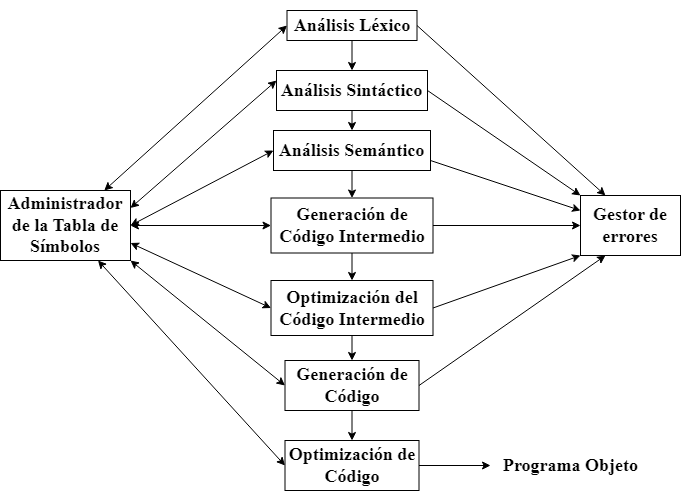
\includegraphics[scale=0.6]{figuras/Cap1/fasescomp.png} \\
    \caption{Fases Principales en el Proceso de Traducción}\label{fig:fases}
\end{figure}

\section{Definición del problema real}

Este proyecto de fin de carrera se enfoca en una tarea crucial: la corrección, mejora y ampliación de ``SimAS: Simuladores de Analizadores Sintácticos'', que es una aplicación desarrollada en java que tiene como objetivo ayudar a la docencia de la asignatura de Procesadores de Lenguajes de tercer curso de la especialidad de Computación del Grado de Ingeniería Informática. 

SimAS proporciona a los estudiantes una comprensión profunda del funcionamiento de la fase de análisis sintáctico en compiladores e intérpretes. Tiene la capacidad de simular tanto analizadores sintácticos descendentes como ascendentes, facilitando que los estudiantes comprendan mejor el funcionamiento de estos métodos de análisis sintáctico.

SimAS es una aplicación de software que posee dos versiones. SimAS 1.0 fue desarrollado por Vanesa González Pérez \cite{vanesa} como Proyecto de Fin de Carrera de Ingeniería Informática en 2015. Esta versión permitía realizar el análisis sintáctico descendente predictivo y el análisis ascendente LR (SLR, LR - canónico y LALR).  Esta versión fue corregida y ampliada en la versión SimAS 2.0, que fue desarrollada por Juan Antonio Fernández Díaz \cite{juan} en su Trabajo de Fin de Grado en 2023. Esta versión permitía generar informes en formato pdf y generar los árboles sintácticos asociados a la derivaciones de los analizadores sintácticos.


A pesar de la funcionalidad satisfactoria de SimAS, se han detectado una serie de errores y deficiencias que demandan atención inmediata.
\begin{itemize}
    \item Al cargar o modificar gramáticas, la aplicación debe ordenar sus reglas de producción en función del símbolo no terminal de la parte izquierda.
    \item Al crear o modificar gramáticas, la aplicación no genera bien el archivo XML \cite{xml} con dicha gramática.
    \item La aplicación no genera o genera de forma incorrecta los informes en formato PDF.
    \item No genera correctamente los conjuntos Primero y Siguiente de algunas gramáticas. Estos conjuntos son necesarios para realizar el análisis sintáctico descendente predictivo y el análisis sintáctico ascendente SLR.
    \item La aplicación no genera correctamente los árboles sintácticos asociados a las derivaciones.
    \item La interfaz produce algunas ventanas no interactivas o que no aportan valor.
\end{itemize}

Además, se pueden incorporar las siguientes mejoras para enriquecer la aplicación:

\begin{itemize}
    \item Diseñar una interfaz más intuitiva que genere todas las ventanas dentro de una misma interfaz y no en diferentes ventanas.
    \item Permitir el trabajo con varias gramáticas a la vez. 
    \item Implementar la posibilidad de cambiar el idioma de la aplicación.
\end{itemize}

Una descripción más detallada de las versiones de SimAS se puede consultar en el capítulo \ref{cap:antecedentes} de Antecedentes.


Aunque las versiones anteriores SimAS 1.0  y 2.0 permiten simular los análisis sintácticos descendente y ascendente, el presente Trabajo de Fin de Grado se va a centrar exclusivamente en corregir todos los fallos encontrados y en mejorar el análisis sintáctico descendente predictivo. La nueva aplicación se denominará ``SimAS 3.0 descendente predictivo''. Se considera que abordar también la corrección de los errores de la simulación del análisis sintáctico ascendente requeriría un esfuerzo superior al exigido en un Trabajo de Fin de Grado. Se debe tener en cuenta que la versión SimAS 2.0 \cite{juan} fue realizada en un Trabajo de Fin de Grado de doble especialidad que tiene una carga docente de 450 horas, superior a las 300 horas de un Trabajo de Fin de Grado de una única especialidad.


\section{Definición del problema técnico}


El presente Trabajo de Fin de Grado pretende desarrollar una aplicación informática multiplataforma, denominada ``SimAS 3.0 descendente predictivo'', que permita corregir y ampliar la simulación del análisis sintáctico descendente predictivo desarrollado en las versiones anteriores de SimAS 1.0 \cite{vanesa} y 2.0 \cite{juan}.

\subsection{Funcionamiento}
La aplicación propuesta se diseñará como una herramienta de escritorio multiplataforma con el objetivo de proporcionar a los usuarios una experiencia interactiva y educativa. Los principales módulos que integrará esta aplicación son los siguientes:

\begin{itemize}
    \item \textbf{Editor de gramáticas de contexto libre:} este módulo permitirá a los usuarios crear, cargar, guardar y modificar gramáticas de contexto libre. La interfaz proporcionará opciones intuitivas para trabajar con las reglas de producción, símbolos terminales y no terminales, así como la definición del símbolo inicial.

    \item \textbf{Simulador gráfico descendente:} esta funcionalidad simulará el proceso de análisis sintáctico descendente predictivo, utilizando la gramática especificada en el editor. El simulador generará una derivación por la izquierda y mostrará el árbol sintáctico descendente resultante.

    \item \textbf{Generación de árboles sintácticos descendentes:} se implementará la funcionalidad para generar árboles sintácticos de forma precisa y visualmente comprensible. Esta característica permitirá a los usuarios visualizar de manera clara la estructura jerárquica de las derivaciones sintácticas.
    
    \item \textbf{Tutorial interactivo:} este módulo proporcionará una guía paso a paso sobre los fundamentos y el funcionamiento de los métodos de análisis sintáctico. Los usuarios podrán acceder a explicaciones detalladas y ejemplos prácticos para comprender mejor los conceptos.
    
    \item \textbf{Ayuda integrada:} se incluirá una sección de ayuda en la interfaz para brindar asistencia instantánea sobre el uso de la aplicación. Los usuarios podrán acceder a información detallada sobre cada componente de la interfaz y los distintos módulos que componen la aplicación.
\end{itemize}

El funcionamiento detallado de cada uno de estos módulos se abordará en el capítulo \ref{cap:especificacion_requisitos} de Especificación de requisitos para proporcionar una comprensión completa de la aplicación.


\subsection{Entorno}
%Posibles modificaciones conforme se desarrolle la aplicación

El entorno en el que se desarrolla y ejecuta una aplicación es fundamental para garantizar su funcionalidad, usabilidad y despliegue efectivo. En este apartado, se detallan los aspectos relacionados con la interfaz de usuario, el entorno de desarrollo y el entorno de ejecución de la aplicación ``SimAS 3.0 descendente predictivo'', proporcionando una visión general de los componentes y requisitos clave para su funcionamiento.


\subsubsection{Interfaz con el usuario}

La aplicación contará con una interfaz gráfica de usuario (GUI\footnote{\textit{Graphical User Interface}}) diseñada para optimizar la experiencia del usuario, especialmente para los estudiantes. Se busca que todo el programa se ejecute en una única ventana, posibilitando la aparición de distintas pestañas, con el fin de simplificar la navegación. 

La interfaz estará diseñada para ser simple y completa al mismo tiempo, permitiendo a los usuarios realizar todas las operaciones necesarias para trabajar con gramáticas. Entre las funcionalidades específicas que ofrecerá la interfaz, se incluyen la capacidad de crear nuevas gramáticas e importar y editar gramáticas creadas previamente. Además, se proporcionará soporte para interacciones complejas, como la entrada de texto y la selección de archivos.

\subsubsection{Entorno de desarrollo}
El desarrollo y mantenimiento del código de la aplicación se realizará utilizando diversas fuentes de información disponibles en Internet, así como técnicas de inteligencia artificial. El entorno de desarrollo integrado (IDE) principal utilizado será IntelliJ \cite{intellij}, que ofrece una amplia gama de características y herramientas para el desarrollo de aplicaciones Java. Además, se utilizarán herramientas adicionales, como sistemas de control de versiones (Git \cite{git}) para el control del código fuente, y se gestionará la documentación y los recursos del proyecto en un repositorio de GitHub \cite{github}.

\subsubsection{Entorno de ejecución}
La aplicación estará diseñada para ser ejecutada en un entorno multiplataforma y compatible con los principales sistemas operativos, incluyendo Windows, macOS y Linux. No se requerirán configuraciones específicas del sistema operativo o del entorno de ejecución para garantizar el funcionamiento correcto de la aplicación. Además, la aplicación se ejecutará en una máquina virtual de Java \cite{java}, lo que proporcionará una mayor portabilidad y compatibilidad con diferentes sistemas. Esto significa que los usuarios finales no necesitarán instalar ninguna dependencia externa ni cumplir con requisitos adicionales de instalación, lo que facilitará su despliegue y uso.


\subsection{Ciclo de mantenimiento} \label{subsec:actualizaciones}

La gestión de actualizaciones de software es un proceso crítico que garantiza la evolución continua y la mejora de la aplicación a lo largo del tiempo. En el caso de ``SimAS 3.0 descendente predictivo'', se implementará un ciclo de mantenimiento diseñado para abordar nuevas funcionalidades, correcciones de errores y adaptaciones a los cambios en los entornos de ejecución.

El ciclo de mantenimiento de ``SimAS 3.0 descendente predictivo'' se basará en un enfoque proactivo y modular, permitiendo la incorporación de mejoras de manera eficiente y sin interrupciones significativas en la experiencia del usuario. Aunque el autor principal del proyecto no asumirá la responsabilidad directa del mantenimiento futuro, se establecerán procedimientos claros para la gestión de actualizaciones, asegurando la continuidad y la calidad del software.

Este enfoque modular no solo facilitará el mantenimiento y la actualización del software, sino que también fomentará la colaboración y la contribución de la comunidad de usuarios y desarrolladores. De esta manera, SimAS 3.0 podrá adaptarse de manera ágil a las necesidades cambiantes de los usuarios y a las demandas del entorno tecnológico.


\subsection{Competencia}

El desarrollo de SimAS 3.0 se sitúa en un contexto de continua evolución y expansión en el ámbito de las herramientas educativas para el análisis sintáctico en la informática. Aunque no buscamos competir comercialmente, es importante comprender el panorama actual y las características distintivas de SimAS 3.0 en relación con otras soluciones disponibles.

A través de un análisis exhaustivo en el Capítulo \ref{cap:antecedentes}, se explorará el terreno de las herramientas educativas existentes para el análisis sintáctico. Se examinarán tanto las aplicaciones desarrolladas en proyectos académicos previos, como otras soluciones disponibles en el mercado. Este análisis permitirá identificar fortalezas, debilidades y oportunidades de mejora para SimAS 3.0.

Si bien se reconocen las contribuciones de otras herramientas educativas, SimAS 3.0 buscará destacarse por su enfoque innovador y sus funcionalidades distintivas. Entre estas funcionalidades, se encuentra la capacidad de generar árboles sintácticos tanto descendentes como ascendentes, ofreciendo una experiencia de aprendizaje única y completa para los estudiantes de informática.


%Posibles modificaciones durante el desarrollo
\subsection{Aspecto externo}

En esta sección, se abordarán aspectos clave relacionados con la experiencia del usuario y la documentación asociada a SimAS 3.0.

\begin{itemize}
    \item \textbf{Diseño de la interfaz de usuario}: la interfaz de usuario de SimAS 3.0 se diseñará cuidadosamente para garantizar una experiencia visual atractiva y una navegación intuitiva. Se prestará especial atención a la disposición de los elementos, la coherencia visual y la accesibilidad, con el objetivo de proporcionar un entorno de trabajo cómodo y eficiente para los usuarios.
    
    \item \textbf{Documentación detallada}:
    \begin{itemize}
        \item \textit{Manual técnico}: este documento proporcionará una descripción exhaustiva de los aspectos técnicos del desarrollo de SimAS 3.0. Se incluirán detalles sobre la arquitectura del software, las tecnologías utilizadas y las decisiones de diseño fundamentales.
        
        \item \textit{Manual de usuario}: el manual de usuario de SimAS 3.0 contendrá instrucciones claras y concisas sobre la instalación, configuración y uso de la aplicación. Se incluirán ejemplos prácticos y capturas de pantalla para guiar al usuario a través de las diferentes funcionalidades de la aplicación.
        
        \item \textit{Manual de código}: este documento estará dirigido a desarrolladores y proporcionará una visión detallada del código fuente de SimAS 3.0. Se describirá la estructura del proyecto, las convenciones de codificación y la documentación interna del código para facilitar su comprensión y mantenimiento.
    \end{itemize}
    
    \item \textbf{Distribución y almacenamiento}: SimAS 3.0 estará disponible para su descarga en línea a través de un repositorio público, lo que facilitará el acceso a la última versión del software y de la documentación asociada. Además, se explorarán opciones para distribuir la aplicación en medios físicos o mediante servicios de almacenamiento en la nube, asegurando así su disponibilidad y accesibilidad para los usuarios.
\end{itemize}


\subsection{Estandarización}

En esta sección, se describirán los principios de diseño y usabilidad que guiarán el desarrollo de SimAS 3.0, con el objetivo de garantizar una experiencia de usuario coherente y satisfactoria.

\begin{itemize}
    \item \textbf{Diseño centrado en el usuario}: SimAS 3.0 se diseñará pensando en las necesidades y expectativas del usuario final. Se realizarán investigaciones de usuarios y pruebas de usabilidad para asegurar que la interfaz de usuario sea intuitiva y fácil de usar.
    
    \item \textbf{Consistencia y coherencia}: la interfaz de usuario de SimAS 3.0 mantendrá una apariencia y comportamiento coherentes en todas sus funciones y elementos. Se seguirán estándares de diseño reconocidos y se aplicarán patrones de diseño comunes para garantizar una experiencia consistente para el usuario.
    
    \item \textbf{Sensibilidad y guía del usuario}: la interfaz de SimAS 3.0 guiará al usuario a través de la aplicación, proporcionando retroalimentación clara y orientación en cada paso del proceso. Se utilizarán mensajes informativos y visuales para informar al usuario sobre el estado y las acciones disponibles.
    
    \item \textbf{Interacción intuitiva}: se priorizará una interacción sencilla y fluida en SimAS 3.0. Los controles y las funciones de la aplicación se diseñarán de manera intuitiva, minimizando la necesidad de aprendizaje por parte del usuario y facilitando el uso de la aplicación desde el primer momento.
    
    \item \textbf{Claridad y legibilidad}: la interfaz gráfica de SimAS 3.0 se diseñará con un enfoque en la claridad y la legibilidad. Se utilizarán colores y tipografías adecuados para garantizar una fácil comprensión de la información presentada, evitando la sobrecarga visual y la confusión del usuario.
\end{itemize}


\subsection{Calidad y fiabilidad}

En esta sección, se abordarán los aspectos de calidad, fiabilidad y seguridad que son fundamentales en el desarrollo y uso de SimAS 3.0. Se buscará garantizar el correcto funcionamiento de la aplicación, así como proteger la integridad y privacidad de los usuarios.

\begin{itemize}
    \item \textbf{Calidad y fiabilidad}: SimAS 3.0 se desarrollará con un enfoque en la calidad del software y la fiabilidad de su funcionamiento. Se utilizarán herramientas actualizadas como IntelliJ IDEA y la Máquina Virtual de Java para respaldar la calidad del código y su ejecución. Además, la aplicación será sometida a exhaustivas pruebas para detectar y corregir errores antes de su lanzamiento.
    
    \item \textbf{Seguridad}: la seguridad de SimAS 3.0 será una prioridad, tanto en términos de protección contra acciones incorrectas por parte del usuario como en la seguridad del dispositivo de almacenamiento. Se implementarán mecanismos de seguridad en la aplicación para evitar cualquier manipulación maliciosa o acceso no autorizado a los datos del usuario. Se garantizará que el usuario no tenga acceso a ninguna funcionalidad aparte de aquellas proporcionadas explícitamente por la aplicación, asegurando así que no se realicen acciones no deseadas ni se acceda a datos sensibles. Asimismo, se garantizará que la distribución y uso de la aplicación cumplan con los principios de software libre, siguiendo la licencia GPL de GNU para proteger su distribución y uso adecuados.
\end{itemize}


\subsection{Validación y verificación}

El proceso de validación y verificación de SimAS 3.0 es esencial para garantizar su correcto funcionamiento y la detección temprana de posibles errores.

\begin{itemize}
    \item \textbf{Validación}: se centrará en asegurar que la aplicación cumple con los requisitos y expectativas del usuario final. Se llevarán a cabo pruebas funcionales para verificar que todas las funcionalidades operan según lo esperado, y se realizarán pruebas de aceptación para garantizar que la aplicación satisface las necesidades del usuario.
    
    \item \textbf{Verificación}: por otro lado, se centrará en asegurar que el código y la lógica de la aplicación son correctos y libres de errores. Se realizarán pruebas unitarias para verificar el correcto funcionamiento de cada componente individualmente, así como pruebas de integración para garantizar que los componentes interactúan correctamente entre sí.
\end{itemize}

El proceso estará dividido en varias etapas, cada una con su respectiva documentación detallada:

\begin{itemize}
    \item \textbf{Planificación de pruebas}: se definirán los objetivos y alcance de las pruebas, así como los recursos y herramientas necesarios para llevarlas a cabo.
    
    \item \textbf{Diseño de pruebas}: se elaborará un plan detallado de las pruebas a realizar, incluyendo los casos de prueba específicos y los criterios de aceptación.
    
    \item \textbf{Ejecución de pruebas}: se llevarán a cabo las pruebas según el plan establecido, registrando los resultados obtenidos y cualquier incidencia detectada.
    
    \item \textbf{Análisis de resultados}: se analizarán los resultados de las pruebas para identificar posibles áreas de mejora o corrección. Se documentarán los errores encontrados y se propondrán soluciones para su resolución.
\end{itemize}

El capítulo \ref{cap:pruebas} detallará cada una de estas etapas y proporcionará una visión completa del proceso de validación y verificación de SimAS 3.0.


\subsection{Programa de tareas}

El desarrollo del Trabajo de Fin de Grado estará compuesto por las siguientes actividades:
\begin{enumerate}
    \item \textbf{Exploración inicial} 
        \begin{itemize}
            \item Comprensión y prueba de SimAS 2.0 \cite{juan}.
            \item Definición del problema técnico.
            \item Establecimiento de los objetivos.
            \item Revisión de los antecedentes.
            \item Identificación de los recursos iniciales y estratégicos.
            \item Selección de las herramientas de software y hardware.
            \item Investigación del entorno Intellij \cite{intellij} y del lenguaje de programación Java \cite{java}.
        \end{itemize}
    \item \textbf{Análisis y diseño}
        \begin{itemize}
            \item Especificación de requisitos: funcionales, no funcionales, de información y de la interfaz.
            \item Elaboración de los casos de uso.
            \item Validación de los casos de uso.
            \item Elaboración de los diagramas de secuencia.
        \end{itemize}
    \item \textbf{Diseño}
        \begin{itemize}
            \item Diseño de la arquitectura del sistema.
            \item Diseño de paquetes y clases.
            \item Diseño de la interfaz
        \end{itemize}        
    \item \textbf{Implementación}
        \begin{itemize}
            \item Desarrollo del código.
            \item Implementación de pruebas unitarias.
            \item Validación del código desarrollado.
        \end{itemize} 
    \item \textbf{Documentación}
      \begin{itemize}
          \item Elaboración del manual técnico, manual de usuario y manual de código.
          \item La redacción del manual técnico se realizará durante todo el proceso de desarrollo del Trabajo de Fin de Grado.
      \end{itemize}
\end{enumerate}

\subsection{Pruebas}
Las pruebas y la validación son elementos esenciales en el desarrollo de cualquier aplicación. Estos procesos permiten asegurar que la aplicación cumpla con los estándares de calidad y funcionalidad esperados. En el caso de SimAS 3.0, se llevarán a cabo diversas actividades de evaluación y validación para garantizar su correcto funcionamiento y fiabilidad.

\subsubsection{Tipos de Pruebas}

Se llevarán a cabo varios tipos de pruebas para evaluar distintos aspectos de SimAS 3.0:

\begin{itemize}
    \item \textbf{Pruebas de Funcionalidad:} estas pruebas se centran en verificar que todas las funciones y características de SimAS 3.0 funcionen como se espera. Se realizarán pruebas exhaustivas para cada módulo y componente de la aplicación.
    
    \item \textbf{Pruebas de Interfaz de Usuario:} estas pruebas se enfocarán en la usabilidad y la experiencia del usuario. Se evaluará la interfaz gráfica para garantizar que sea intuitiva y fácil de usar.

    \item \textbf{Pruebas de Rendimiento:} se llevarán a cabo pruebas para evaluar el rendimiento y la velocidad de SimAS 3.0, especialmente en situaciones de carga y con grandes conjuntos de datos.

    \item \textbf{Pruebas de Compatibilidad:} se realizarán pruebas en diferentes sistemas operativos y entornos de ejecución para garantizar que SimAS 3.0 funcione correctamente en diversas configuraciones.
\end{itemize}

\subsubsection{Descripción de las Pruebas}

Cada prueba estará estructurada de la siguiente manera:

\begin{itemize}
    \item \textbf{Objetivo:} se definirá claramente el objetivo de la prueba, es decir, qué se espera evaluar o validar.
    
    \item \textbf{Problema:} se identificarán y documentarán los problemas o errores detectados durante la ejecución de la prueba, junto con información detallada sobre cómo reproducirlos.

    \item \textbf{Solución:} se propondrán soluciones y acciones correctivas para abordar los problemas identificados durante las pruebas, asegurando así la mejora continua de la aplicación.
\end{itemize}

El próximo capítulo \ref{cap:pruebas} detallará los procedimientos y resultados de las pruebas llevadas a cabo en ``SimAS 3.0 descendente predictivo'' como parte de este Trabajo de Fin de Grado.


\subsection{Seguridad}
La seguridad en la presente aplicación se centra principalmente en garantizar su correcto funcionamiento sin comprometer la integridad de los sistemas donde se ejecute. Dado que la aplicación no maneja ni almacena datos personales de los usuarios, el enfoque de seguridad se orienta hacia la prevención de posibles daños a los equipos o entornos de ejecución.

Se implementarán medidas para asegurar que durante la ejecución de la aplicación, los usuarios no puedan realizar acciones que puedan comprometer su funcionamiento o la estabilidad del sistema. Además, se prestará especial atención a la protección del dispositivo de almacenamiento donde se ejecute la aplicación, garantizando que no se produzcan daños o alteraciones no deseadas.

En línea con la versión anterior, la aplicación se distribuirá libremente, sin restricciones de uso, copia o distribución. Esto se fundamenta en su naturaleza académica y en su carácter no lucrativo. No se aplicarán medidas de protección contra la distribución libre de la aplicación, permitiendo su acceso y uso por parte de cualquier usuario interesado en aprender o utilizarla con fines educativos.

En cuanto a la licencia, la aplicación seguirá los principios de la Licencia Pública General de GNU (GPL), que garantiza la libertad de uso, modificación y redistribución del software. Esta licencia ayuda a prevenir acciones malintencionadas relacionadas con la copia o reproducción del software, asegurando que permanezca accesible para la comunidad académica y de desarrollo de software.
\chapter{Objetivos} \label{cap:objetivos}
\section{Objetivo principal}

El objetivo principal de este Trabajo de Fin de Grado es desarrollar la aplicación informática ``SimAS 3.0 descendente predictivo'', que permita la simulación de analizadores sintácticos descendentes predictivos, así como la generación de árboles sintácticos asociados a sus derivaciones sintácticas.

\section{Objetivos específicos}

El objetivo principal se desglosa en los siguientes objetivos específicos:

\begin{itemize}
    \item Revisar la versión anterior de SimAS 2.0 \cite{juan} para identificar y corregir errores y deficiencias del análisis sintáctico descendente predictivo,  tales como:
    \begin{itemize}
        \item Mejorar la edición  y el almacenamiento de gramáticas de contexto libre.
        \item Depurar la validación automática de gramáticas de contexto libre: comprobar que la gramática no tiene símbolos inútiles.
        \item Permitir la visualización de las gramáticas originales y transformadas.
        \item Definir funciones para el tratamiento automático de errores.
        \item Garantizar la simulación correcta de gramáticas que incluyan reglas épsilon.
        \item Generar correctamente los conjuntos Primero y Siguiente.
        \item Asegurar la generación adecuada de informes en formato PDF.
    \end{itemize}
    \item Ampliar las capacidades de SimAS para incluir la generación de árboles sintácticos de las derivaciones producidas por los analizadores sintácticos descendente predictivos:
    \begin{itemize}
        \item Permitir la generación paso a paso de los árboles sintácticos asociados a las derivaciones.
        \item Facilitar la exportación de los árboles sintácticos generados en diversos formatos.
    \end{itemize}
\end{itemize}


\section{Objetivos personales}

En el ámbito personal y profesional, se plantean los siguientes objetivos a alcanzar durante el desarrollo de este Trabajo de Fin de Grado:

\begin{itemize}
    \item \textbf{Contribuir a la educación en informática:} desarrollar una aplicación informática que no solo cumpla con los requisitos académicos del proyecto, sino que también pueda utilizarse como herramienta educativa en el ámbito de la enseñanza de los analizadores sintácticos. Se busca que esta aplicación sea útil para estudiantes y profesores en el aprendizaje y la enseñanza de este tema fundamental.
    
    \item \textbf{Profundizar en Java y Java Swing:} aprovechar este proyecto como una oportunidad para mejorar mis habilidades en el lenguaje de programación Java y en el uso de sus bibliotecas, especialmente Java Swing \cite{javaswing}. Se busca obtener un conocimiento más sólido y práctico en el desarrollo de aplicaciones gráficas de usuario, lo que puede ser beneficioso para futuros proyectos y oportunidades profesionales.

    \item \textbf{Explorar otras herramientas de desarrollo:} esta tarea implica investigar y adquirir conocimientos sobre diversas herramientas y tecnologías utilizadas en el desarrollo de aplicaciones informáticas, además de Java y Java Swing. Entre estas herramientas, un ejemplo destacado es Scene Builder \cite{scenebuilder}. Scene Builder es una herramienta gráfica que permite diseñar interfaces de usuario de manera intuitiva y visual, utilizando la tecnología JavaFX. Permite arrastrar y soltar componentes de la interfaz gráfica, configurar propiedades y establecer el diseño de la aplicación de forma rápida y eficiente. Explorar y familiarizarse con herramientas como Scene Builder amplía el repertorio de herramientas disponibles para el desarrollo de interfaces de usuario, lo que permite evaluar y seleccionar las mejores soluciones para proyectos futuros.
    
    \item \textbf{Aprender sobre el ciclo de desarrollo de software:} obtener una comprensión más profunda del proceso de desarrollo de software, desde la planificación y el diseño hasta la implementación, las pruebas y la documentación. Se busca adquirir experiencia práctica en todas las etapas del ciclo de vida del desarrollo de software y aprender a aplicar metodologías y buenas prácticas de ingeniería de software en un proyecto real.
\end{itemize}
\chapter{Antecedentes}\label{cap:antecedentes}

\section{Introducción}

Este capítulo proporcionará una visión general de los antecedentes que contextualizan el desarrollo del presente Trabajo de Fin de Grado. 

En primer lugar, se abordarán aspectos teóricos del análisis sintáctico para comprender mejor el marco conceptual en el que se enmarca este trabajo (Sección \ref{sec:fundamentos}). 


A continuación, se llevará a cabo un análisis exhaustivo de la versión anterior de la aplicación SimAS 2.0, la cual se basa en la versión original SimAS 1.0 (Sección \ref{sec:SimAs1.0}) desarrollada por Vanesa Martínez García \cite{vanesa}. La versión 2.0 fue desarrollada por Juan Antonio Fernández Díaz \cite{juan} en 2023. En este análisis se examinarán en detalle las funcionalidades principales de SimAS 2.0, así como los desafíos y limitaciones encontrados en su implementación (Sección \ref{sec:SimAs2.0}).

Por último, se presentarán las razones y justificaciones que respaldan la realización de este Trabajo de Fin de Grado. Se discutirá la necesidad de mejorar y ampliar las capacidades de la aplicación SimAS para proporcionar una herramienta más eficaz y completa para el aprendizaje del análisis sintáctico en el contexto académico (Sección \ref{sec:justificacion}).


\section{Fundamentos teóricos del análisis sintáctico}\label{sec:fundamentos}

\subsection{Tipos de analizadores sintácticos}

 El análisis sintáctico es una fase muy importante del proceso de traducción o interpretación de un programa escrito en un lenguaje de programación. Existen diferentes tipos de analizadores sintácticos: generales, descendentes y ascendentes. El presente Trabajo de Fin de Grado simulará el funcionamiento de algunos analizadores sintácticos descendentes y ascendentes, que se describen, brevemente, en las secciones \ref{sec:descendente} y \ref{sec:ascendente}, respectivamente.

 Los analizadores sintácticos están basados en un tipo de gramática formal, denominada \textit{gramática independiente del contexto} o \textit{gramática de contexto libre}, que permite generar muchos aspectos de los lenguajes de programación. Las características de las gramáticas de contexto libre se describen en la sección \ref{sec:gramatica-contexto-libre}. 

 Una descripción más detallada del los fundamentos teóricos del análisis sintáctico se puede consultar en el libro de A. V. Aho et al. \cite{aho2008}.
 
 \subsection{Gramáticas de contexto libre}\label{sec:gramatica-contexto-libre}


\begin{definicion}
 Una {\bf\em gramática de contexto libre} $G$ se define como
\begin{equation}
    G = (V_N, V_T,P,S)
\end{equation}
donde
\begin{itemize}
\item $V_N$ es un conjunto finito de símbolos que se denomina {\bf\em vocabulario o alfabeto no terminal} y también puede ser denotado por $\Sigma_N$ o $N$.
\item $V_T$ es un conjunto finito de símbolos que se denomina {\bf\em  vocabulario o alfabeto terminal} y también puede ser denotado por $\Sigma_T$ o $T$,
\item $S \in V_N$ y es el {\bf\em axioma} o {\bf\em símbolo inicial o distinguido} de la gramática  y
\item $P$ es el {\bf\em conjunto de reglas de reescritura o de  producción}. 
\end{itemize}

 Se verifica que 
\begin{eqnarray}
    V_N \cup V_T = V \\
    V_N \cap V_T = \emptyset
\end{eqnarray}

 $V$ es el {\bf\em alfabeto o vocabulario} de la gramática y también suele ser denotado por $\Sigma$.

 El conjunto de producciones $P$ se define como 
\begin{equation}
  P = \{ (A, \beta) | A \in V_N, \beta \in V^* = (V_N \cup V_T)^* \}
\end{equation}

 El par $(A \beta)$ suele ser denotado por 
\begin{equation}
  A \rightarrow \beta
\end{equation}
siendo $A$ la parte izquierda de la regla de producción y $\beta$ la parte derecha.
\end{definicion}

 Las gramáticas de contexto libre también se denominan \textit{gramáticas independientes del contexto} o \textit{gramáticas de tipo 2} según la jerarquía de Noam Chomsky \cite{aho2008}.

 Muchas de las sentencias de los lenguajes de programación pueden ser generadas por gramáticas de contexto libre. En el siguiente ejemplo, se muestra una gramática que permite generar sentencias de asignación de expresiones numéricas a un identificador.
 
Sea la gramática de contexto libre $G = (V_N, V_T,P,S)$ donde
\begin{itemize}
\item $V_N = \{S, E\}$
\item $V_T = \{\mbox{\bf\em identificador}, =, +, *, (, ), \mbox{\bf\em número}\}$
\item $S \in V_N$
\item y el conjunto de reglas de producción es:
\begin{eqnarray*}
  P & = & \{ \\
     & (1) & S \longrightarrow \mbox{\bf\em identificador } = \hspace{1ex} E \\
     & (2) & E \longrightarrow E \hspace{1ex} + \hspace{1ex} E \\
     & (3) & E \longrightarrow E \hspace{1ex} * \hspace{1ex} E \\
     & (4) & E \longrightarrow ( \hspace{1ex} E \hspace{1ex} ) \\
     & (5) & E \longrightarrow \mbox{\bf\em identificador} \\
     & (6) & E \longrightarrow \mbox{\bf\em número} \\ 
     &   &\}
\end{eqnarray*}
\end{itemize}


\subsection{Derivación con una gramática de contexto libre}
 
 Las gramáticas de contexto libre utilizan el concepto de derivación para generar las palabras de una lenguaje de contexto libre. A continuación, se define los conceptos de \textbf{derivación inmediata} y \textbf{derivación general} o, simplemente, \textbf{derivación}.

\begin{definicion}
Si $G = (V_N,V_T,P,S)$ es una gramática de contexto libre, $\delta A \eta$ es una cadena de símbolos donde $A \in V_N$ y $\delta, \eta \in V^*$ y $A \longrightarrow \beta$ es una regla de producción de la gramática entonces
\begin{equation}  
  \delta A \eta \Dflecha_G \delta \beta \eta 
\end{equation}  
 es una {\bf\em derivación inmediata} realizada una producción de la gramática $G$.
\end{definicion}

Una derivación inmediata de una gramática de contexto libre solamente sustituye un símbolo no terminal por una cadena de símbolos que formen la parte derecha de alguna de sus reglas.

\begin{definicion}
 Una {\bf\em derivación} es una secuencia de cadenas $\alpha_0, \alpha_1, \dots, \alpha_n$ $(n \geq 0)$, de forma que la cadena $\alpha_{i+1} = \delta \beta_i \eta$ se obtiene mediante una derivación inmediata de la cadena $\alpha_i = \delta A_i \eta \hspace{1ex} (0 \leq i \leq n-1)$, es decir,
\begin{equation}
 \alpha_i = \delta  A_i \eta \Dflecha_G \delta \beta_i \eta = \alpha_{i+1} 
\end{equation}
donde $A_i \in V_N$ y $\delta,\eta,\beta_i \in V^*$.

Encadenando todas las derivaciones inmediatas, se tiene que 
\begin{equation}
 \alpha_0 \Dflecha_G \alpha_1 \Dflecha_G \alpha_2 \Dflecha_G \dots \Dflecha_G \alpha_i \Dflecha_G  \alpha_{i+1} \Dflecha_G  \dots \Dflecha_G  \alpha_n
\end{equation}
o, abreviadamente,
\begin{equation}
\alpha_0 \Dflecha^*_G \alpha_n
\end{equation}
 indicando que $\alpha_0$ deriva a $\alpha_n$ en cero o m\'as pasos o derivaciones inmediatas.
\end{definicion}

\begin{itemize}
\item Siempre se verifica que 
\begin{equation}
 \alpha \Dflecha^0_G \alpha
\end{equation}
\item Si $n \geq 1$ entonces 
\begin{equation}
 \alpha_0 \Dflecha^+_G \alpha_n
\end{equation}
En este caso, $\alpha_0$ deriva a $\alpha_n$ en uno o m\'as pasos o derivaciones inmediatas.
\item Si 
\begin{equation}
 \alpha \Dflecha^n_G \beta
\end{equation}
entonces se dice que $\alpha$ deriva a $\beta$ en $n$ pasos o derivaciones inmediatas.
\item Una {\bf\em derivación} es {\bf\em inicial} si $\alpha_0 = S$.
\item Una {\bf\em derivación} es {\bf\em terminal} si a partir de $\alpha_n$  no se puede aplicar ninguna regla de la gramática.
\end{itemize}


La gramática definida en la sección \ref{sec:gramatica-contexto-libre} permite generar la siguiente derivación que corresponde a una sentencia de asignación de una expresión aritmética:

\begin{eqnarray*}
  S  & \Dflecha_1 & \mbox{\bf\em identificador } = \hspace{1ex} E \\
     & \Dflecha_2 & \mbox{\bf\em identificador } = \hspace{1ex} E \hspace{1ex} + \hspace{1ex} E \\
     & \Dflecha_3 & \mbox{\bf\em identificador } = \hspace{1ex} E \hspace{1ex} + \hspace{1ex} E \hspace{1ex} * \hspace{1ex} E \\
     & \Dflecha_6 & \mbox{\bf\em identificador } = \hspace{1ex} E \hspace{1ex} + \hspace{1ex} \mbox{\bf\em número } * \hspace{1ex} E \\
     & \Dflecha_5 & \mbox{\bf\em identificador } = \hspace{1ex} E \hspace{1ex} + \hspace{1ex} \mbox{\bf\em número } * \hspace{1ex} \mbox{\bf\em identificador }  \\
     & \Dflecha_5 & \mbox{\bf\em identificador } = \mbox{\bf\em identificador } + \hspace{1ex} \mbox{\bf\em número } * \hspace{1ex} \mbox{\bf\em identificador } 
\end{eqnarray*}

Algunas derivaciones se pueden clasificar a su vez en dos categorías: \textbf{derivación por la izquierda} y \textbf{derivación por la derecha}.

\begin{definicion}
 Se dice que una {\bf\em derivación} $\alpha_0, \alpha_1, \dots, \alpha_n \hspace{1ex} (n \geq 0)$, es por la {\bf\em izquierda} si $\forall i \in \{0, \dots, n-1\} \hspace{1ex} \exists A_i \longrightarrow \beta \in P$  tal que
\begin{equation}
 \alpha_i = x  A_i \eta \Dflecha_I x \beta_i \eta = \alpha_{i+1} 
\end{equation}
 donde $x \in V^*_T, A_i \in V_N$ y $\eta, \beta \in V^* = (V_N \cup V_T)^*$
\end{definicion}

 Las derivaciones por la izquierda siempre aplican, en cada paso o derivación inmediata, una regla asociada al símbolo no terminal situado más a la izquierda. La definición de derivación por la derecha es análoga.

El siguiente ejemplo muestra la derivación por la izquierda correspondiente a la derivación general del ejemplo anterior.

\begin{eqnarray*}
  S  & \Dflecha_1 & \mbox{\bf\em identificador } = \hspace{1ex} E \\
     & \Dflecha_2 & \mbox{\bf\em identificador } = \hspace{1ex} E \hspace{1ex} + \hspace{1ex} E \\
     & \Dflecha_5 & \mbox{\bf\em identificador } = \mbox{\bf\em identificador} \hspace{1ex} + \hspace{1ex} E \\
     & \Dflecha_3 & \mbox{\bf\em identificador } = \mbox{\bf\em identificador }  + \hspace{1ex} E \hspace{1ex} * \hspace{1ex} E \\
     & \Dflecha_6 & \mbox{\bf\em identificador } = \mbox{\bf\em identificador } + \hspace{1ex} \mbox{\bf\em número } * \hspace{1ex} E \\
     & \Dflecha_5 & \mbox{\bf\em identificador } = \mbox{\bf\em identificador } + \hspace{1ex} \mbox{\bf\em número } * \hspace{1ex} \mbox{\bf\em identificador } 
\end{eqnarray*}


\subsection{Árbol de derivación o árbol sintáctico}

El \textbf{árbol de derivación} o \textbf{árbol sintáctico} asociado a una \textbf{derivación} de una gramática de contexto libre es un árbol sintáctico que posee las siguientes características:
\begin{enumerate}
\item Los nodos del árbol están etiquetados con símbolos gramaticales (terminales o no terminales) o con la palabra vacía.
\item La raíz del árbol está etiquetada con el símbolo inicial de la gramática.
\item Si un nodo tiene al menos un descendiente, le corresponde como etiqueta un símbolo no terminal.
\item Si tenemos un nodo etiquetado con $A$ y se ha aplicado la regla $A \longrightarrow X_1 X_2 \dots X_k$, donde $X_i \in V \cup \{\epsilon\} \hspace{1ex} \forall i \in \{1,2,\dots,k\}$, entonces dicho nodo tendrá $k$ descendientes inmediatos (``hijos'') etiquetados con los símbolos $X_1, X_2, \dots, X_k$.
\end{enumerate}

La figura \ref{fig-arbol-derivacion-gramatica-contexto-libre} muestra el árbol correspondiente a la derivación del ejemplo de la sección anterior.

\begin{figure}[htp]
\centering
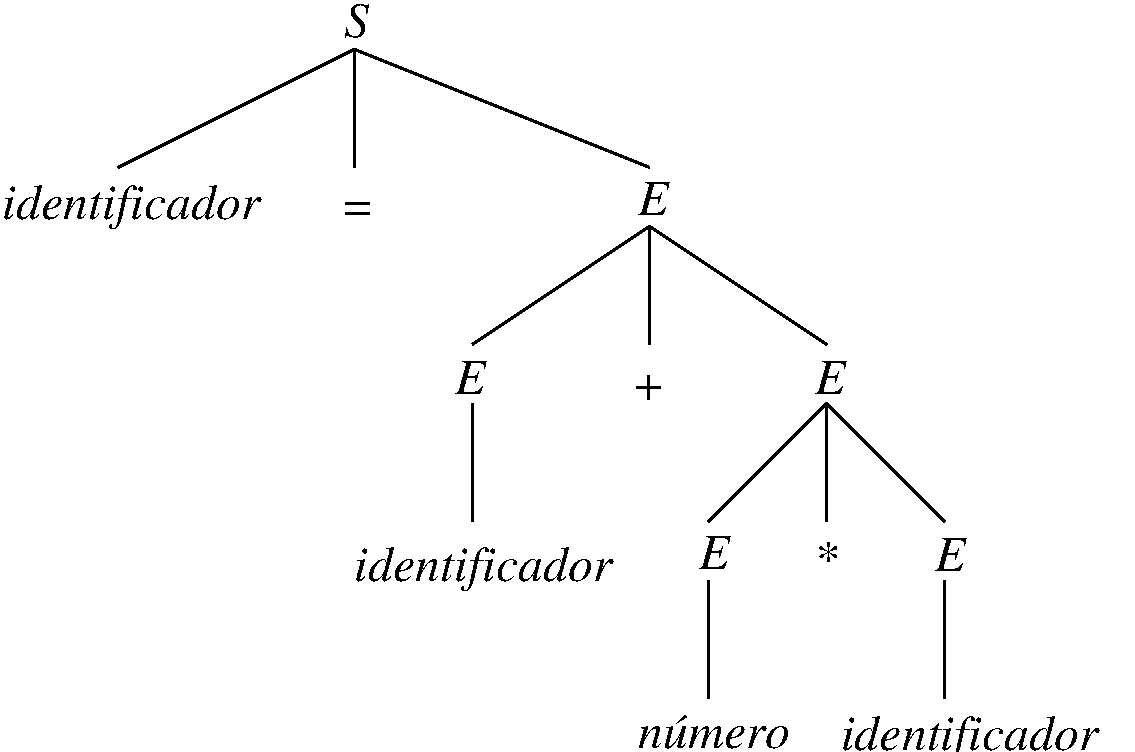
\includegraphics[scale=0.5]{figuras/Cap3/arbol-derivacion-gramatica-contexto-libre.pdf}
 \caption{Ejemplo de árbol sintáctico asociado a una derivación de una gramática de contexto libre.}\label{fig-arbol-derivacion-gramatica-contexto-libre}
\end{figure}


\subsection{Analizadores sintácticos descendentes}\label{sec:descendente}

El análisis sintáctico descendente comprueba si una gramática de contexto libre puede generar la cadena de símbolos de  entrada, como, por ejemplo, una sentencia de un lenguaje de programación, utilizando alguna de las siguientes {\bf estrategias}, que son complementarias:
\begin{itemize}
\item Construcción de una \textbf{derivación por la izquierda} de la cadena de entrada.
\item Construcción de un \textbf{árbol sintáctico} de forma \textbf{descendente} desde la raíz hasta las hojas.
\end{itemize}

Considérese la siguiente gramática que genera sentencias de asignación de expresiones aritméticas:

\begin{eqnarray*}
  P & = & \{ \\
     & (1) & S \longrightarrow \mbox{\bf\em identificador } = \hspace{1ex} E \\
     & (2) & E \longrightarrow T \hspace{1ex} E' \\
     & (3) & E' \longrightarrow + \hspace{1ex} T \hspace{1ex} E' \\
     & (4) & E' \longrightarrow \epsilon \\     
     & (5) & T \longrightarrow F \hspace{1ex} T' \\
     & (6) & T' \longrightarrow * \hspace{1ex} F \hspace{1ex} T' \\
     & (7) & T' \longrightarrow \epsilon \\     
     & (8) & F \longrightarrow ( \hspace{1ex} E \hspace{1ex} ) \\
     & (9) & F \longrightarrow \mbox{\bf\em identificador} \\
     & (10) & F \longrightarrow \mbox{\bf\em número} \\ 
     &   &\}
\end{eqnarray*}

Esta gramática permite generar la siguiente derivación por la izquierda.

\begin{center}
$
\begin{array}{lll}
  S & \Dflecha_1 & {\bf identificador =} \ E \\
   & \Dflecha_2 & {\bf identificador =} \ T E' \\
   & \Dflecha_5 & {\bf identificador =} \ F T' E' \\
   & \Dflecha_9 & {\bf identificador = identificador} T' E' \\
   & \Dflecha_7 & {\bf identificador = identificador \ \epsilon} \  E' \\
   & \Dflecha_3 & {\bf identificador = identificador \ \epsilon \ +} \ T E' \\
   & \Dflecha_5 & {\bf identificador = identificador \ \epsilon \ +} \ F T' E' \\
   & \Dflecha_{10} & {\bf identificador = identificador \ \epsilon \ + n} \ T' E' \\
   & \Dflecha_6 & {\bf identificador = identificador \ \epsilon \ + n \ *} \ F T' E'  \\
   & \Dflecha_9 & {\bf identificador = identificador \ \epsilon \ + n \ * \ identificador} \ T' E' \\
   & \Dflecha_7 & {\bf identificador = identificador \ \epsilon \ + n \ * \ identificador \ \epsilon} \ {E'} \\
   & \Dflecha_4 & {\bf identificador = identificador \ \epsilon \ + n \ * \ identificador \ \epsilon} \ \underline{\epsilon } 
\end{array}
$
\end{center}

Las Figuras \ref{fig:pasos-2-analisis-descendente-predictivo} y \ref{fig:pasos-final-analisis-descendente-predictivo} muestran el paso inicial y final, respectivamente, del árbol sintáctico generado por el análisis descendente. Este árbol invertido ha sido generado de forma descendente desde la raíz hasta la hojas.

\begin{figure}[!t]
    \centering
        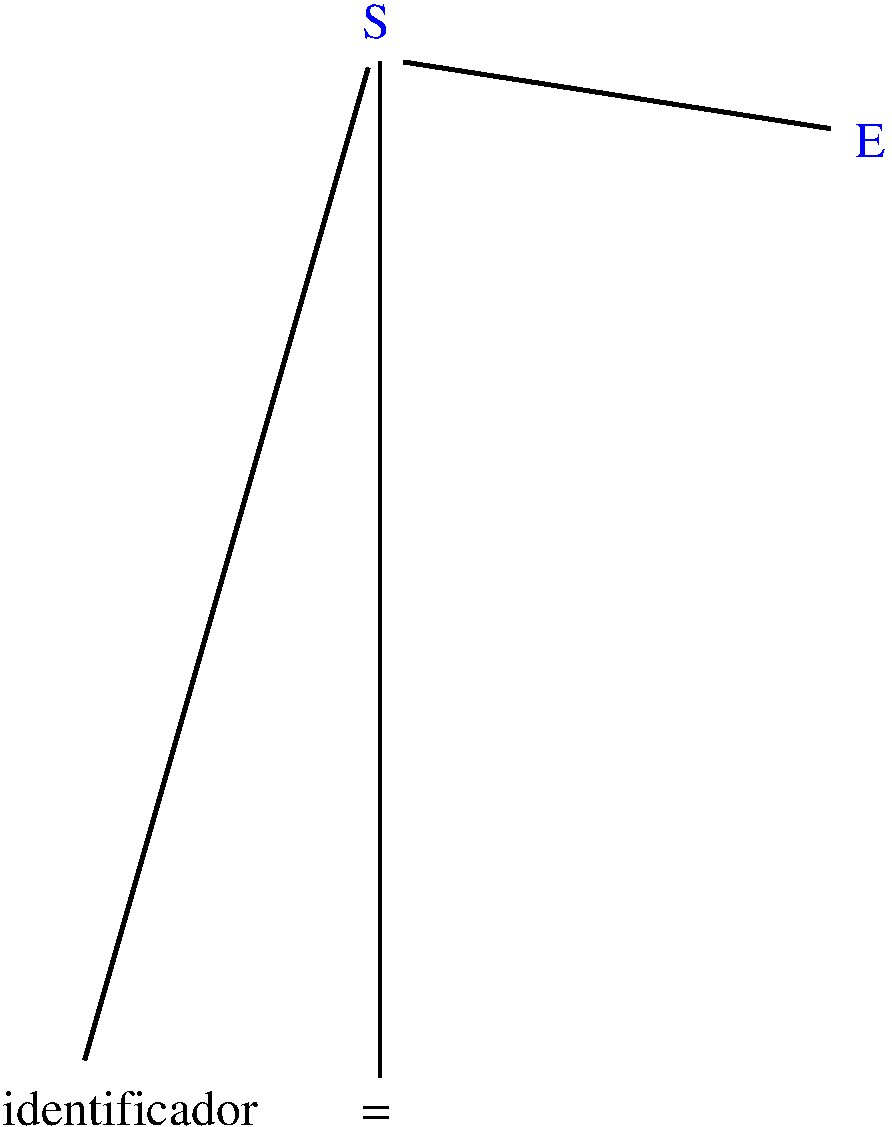
\includegraphics[scale=0.40]{figuras/Cap3/Paso-2-arbol-derivacion-descendente.pdf}
    \caption{Árbol sintáctico: paso inicial del análisis sintáctico descendente predictivo}\label{fig:pasos-2-analisis-descendente-predictivo}
\end{figure}


\begin{figure}[!t]
    \centering
        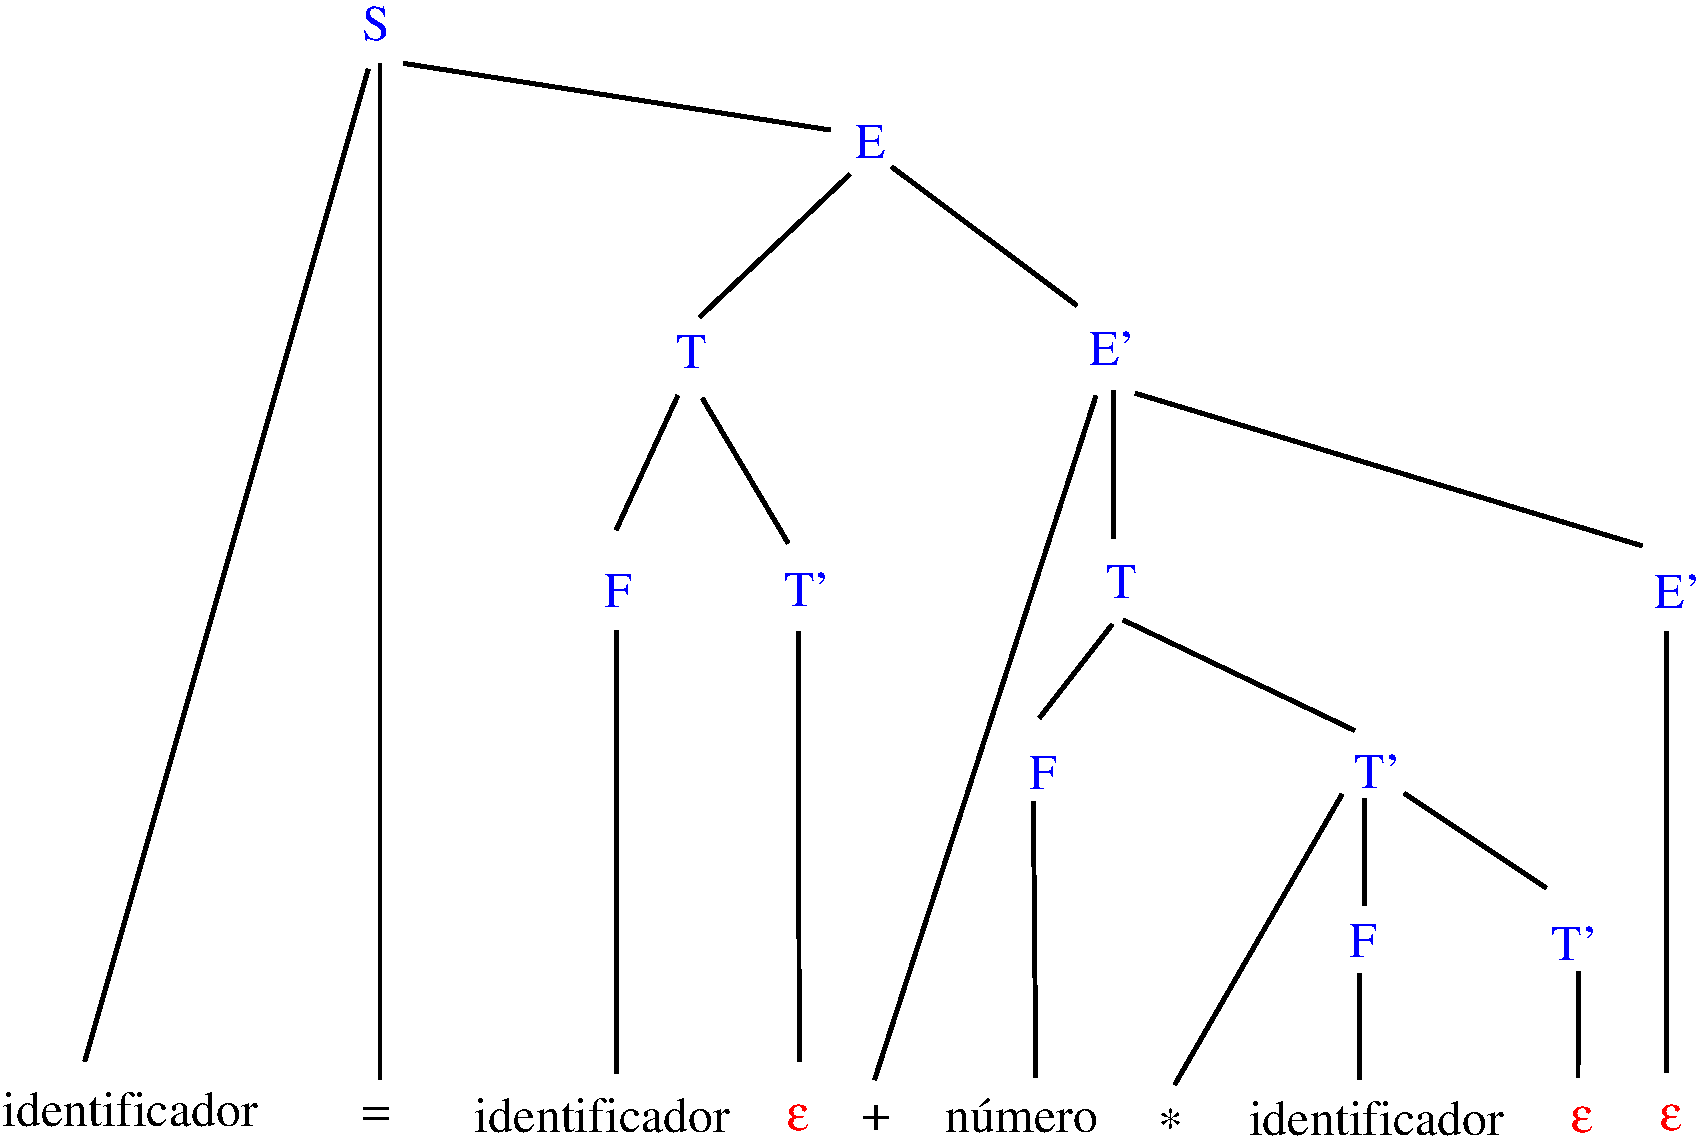
\includegraphics[scale=0.40]{figuras/Cap3/Paso-13-arbol-derivacion-descendente.pdf}
    \caption{Árbol sintáctico: paso final del análisis sintáctico descendente predictivo}\label{fig:pasos-final-analisis-descendente-predictivo}
\end{figure}

Existen diferentes dos tipos de analizadores sintácticos descendentes \cite{aho2008}:
\begin{enumerate}
    \item  Método de descenso recursivo \textbf{con} retroceso o \textit{backtracking}.
    \item Método de descenso \textbf{predictivo}, es decir, \textbf{sin} retroceso.
\end{enumerate}

A su vez, existen dos versiones del análisis descendente predictivo: 
\begin{itemize}
    \item Versión recursiva, que utiliza funciones asociadas a los símbolos no terminales de la gramática de contexto libre.
    \item Versión iterativa, que utiliza una pila para simular el análisis sintáctico descendente.
\end{itemize}

Ambas versiones del análisis descendente predictivo utilizan una \textbf{tabla predictiva} para generar la derivación por la izquierda o el árbol sintáctico de forma descendente.  La Tabla \ref{tabla-analisis-descendente-predictivo} muestra la Tabla de análisis descendente predictivo de la gramática que genera sentencias de asignación de expresiones aritméticas y que se definió previamente.

\begin{table}[htp]
    \centering
    \caption{Tabla de análisis descendente predictivo}
    \label{tabla-analisis-descendente-predictivo}
    \begin{tabular}{|| c || c | c | c | c | c | c | c | c ||} 
      \hline
                  & \multicolumn{8}{c||}{\bf Símbolo de entrada} \\
      \hline 
      \hline 
                  & \textbf{id} & \textbf{=} & \textbf{+} & \textbf{*} & \textbf{(} & \textbf{)} & \textbf{número} & \textbf{\$}  \\ 
      \hline             
      \hline S    &     1       &            &            &            &            &            &                 &  \\ 
      \hline E    &     2       &            &            &            &      2     &            &       2         & \\ 
      \hline E'   &             &            &      3     &            &            &      4     &                 &   4    \\ 
      \hline T    &     5       &            &            &            &      5     &            &       5         &  \\ 
      \hline T'   &             &            &      7     &     6      &            &      7     &                 &  7  \\ 
      \hline F    &     9       &            &            &            &      8     &            &       10        & \\
      \hline
    \end{tabular}
    
\end{table}    

El primer símbolo de cada fila es un símbolo no terminal de la gramática. El primer símbolo de cada columna es o un símbolo terminal de la gramática o el símbolo \$, que representa el fin de la cadena de símbolos que se va a analizar en la entrada. El número que aparece en las celdas interiores de la tabla representa el número de la regla de producción de la gramática que se debe utilizar cuando se está derivando un símbolo no terminal y en la entrada aparece un símbolo terminal o el símbolo \$.

La Tabla \ref{tab:tabla-analisis-descendente-predictivo} muestra cómo se utiliza la Tabla \ref{tabla-analisis-descendente-predictivo} para realizar  el análisis descendente predictivo de la siguiente sentencia:  \textbf{id = id + n * id \$}. La columna \textbf{Acción} de dicha tabla indica las reglas de producción que se deben utilizar para generar la derivación por la izquierda y el árbol sintáctico de forma descendente. Véanse las Figuras \ref{fig:pasos-2-analisis-descendente-predictivo} y \ref{fig:pasos-final-analisis-descendente-predictivo}.

\begin{table}[!t]
\caption{Pasos del análisis descendente predictivo}
    \label{tab:tabla-analisis-descendente-predictivo}
    \centering
\begin{tabular}{l|l|l}
      \hline 
      \textbf{Pila}  \hspace{10ex}                     & \textbf{Entrada}  \hspace{7ex}         & \textbf{Acción} \hspace{8ex}  \\
      \hline 
       {\bf \$} {S}                              & \textbf{ {id} = id + n * id \$}  & 1) S $\rightarrow$ {\bf identificador} {\bf =}  E     \\
       {\bf \$} \underline{E  {\bf =} {\bf id}}  & \textbf{ {id} = id + n * id \$}  & Emparejar   \\
       {\bf \$}  E  {\bf = }                     & \textbf{ {=} id + n * id \$}     & Emparejar   \\
       {\bf \$}  {E}                             & \textbf{ {id} + n * id \$}       & 2) E $\rightarrow$ T E'    \\
       {\bf \$}  \underline{E' {T}}              & \textbf{ {id} + n * id \$}       & 5) T $\rightarrow$ F T'     \\
       {\bf \$}  E' \underline{T' {F}}           & \textbf{ {id} + n * id \$}       & 9) F $\rightarrow$ {\bf identificador}   \\
       {\bf \$}  E' T' \underline{{\bf id}}      & \textbf{ {id} + n * id \$}       & Emparejar \\
       {\bf \$}  E' {T'}                         & \textbf{ {+} n * id \$}          & 7) T' $\rightarrow$ $\epsilon$ \\
       {\bf \$}  {E'}                            & \textbf{ {+} n * id \$}          & 3) E' $\rightarrow$ {\bf +} T E' \\
       {\bf \$} \underline{E' T  {\bf +}}        & \textbf{ {+} n * id \$}          & Emparejar \\
        {{{\bf \$} E' {T}}}  &  {{\textbf{ {n} * id \$}}}     &  \\
        {\bf \$} E' \underline{T' {F}}           &  \textbf{ {n} * id \$}          &  10) F $\rightarrow$ {\bf número} \\
        {\bf \$} E' \underline{T' {\bf n}}       &  \textbf{ {n} * id \$}          & Emparejar  \\
        {\bf \$} E' {T'}                         & \textbf{ {*}  id \$}            & 6) T' $\rightarrow$ {\bf *} F T' \\
        {\bf \$} E' \underline{T' F {\bf *}}     & \textbf{ {*}  id \$}            & Emparejar \\
        {\bf \$} E' T' {F}                       & \textbf{ {id} \$}               &  9) F $\rightarrow$ {\bf identificador} \\
        {\bf \$} E' T' \underline{{\bf id}}      & \textbf{ {id} \$}               &  Emparejar  \\
        {\bf \$} E' {T'}                         & \textbf{ {\$}}                  & 7) T' $\rightarrow$ $\epsilon$ \\
        {\bf \$} {E'}                            & \textbf{ {\$}}                  & 4) E' $\rightarrow$ $\epsilon$ \\
        {\bf \$}                                 & \textbf{ {\$}}                  &  Aceptar\\
       \hline
    \end{tabular}
\end{table}

%\newpage

\subsection{Analizadores sintácticos ascendentes} \label{sec:ascendente}

El análisis sintáctico ascendente comprueba si una gramática de contexto libre puede generar la cadena de símbolos de  entrada, como, por ejemplo, una sentencia de un lenguaje de programación, utilizando alguna de las siguientes {\bf estrategias}, que son complementarias:
\begin{itemize}
\item Construcción de una \textbf{derivación por la derecha en orden inverso} de la cadena de entrada.
\item Construcción de un \textbf{árbol sintáctico} de forma \textbf{ascendente} desde las hojas hasta la raíz.
\end{itemize}


Se han propuesto diferentes métodos de análisis sintáctico ascendente \cite{aho2008}:
\begin{itemize}
 \item Métodos basados en la precedencia
    \begin{itemize}
    \item Métodos de precedencia simple.
    \item Métodos de precedencia débil.
    \item Métodos de precedencia extendida.
    \item Métodos de precedencia de estrategia mixta.
    \item Métodos de precedencia de operadores.
\end{itemize}
 \item Métodos de análisis LR
  \begin{itemize}
      \item Método SLR
      \item Método LR - canónico
      \item Método LALR
  \end{itemize}
\end{itemize}

%En el presente Trabajo de Fin de Grado, solamente se van a considerar los métodos de análisis LR. 
A continuación se muestra un ejemplo de aplicación del método de análisis sintáctico ascendente SLR. Considérese la siguiente gramática de contexto libre que permite generar prototipos de funciones:
\begin{center}
\begin{itemize}
      \item[] {P}  =  \{  
        \begin{itemize}
         \item[(1)] S $\rightarrow$ T {\bf id (} L {\bf ) ;} 
         \item[(2)] T $\rightarrow$ T {\bf *}
         \item[(3)] T $\rightarrow$ {\bf int} 
         \item[(4)] L $\rightarrow$ L {\bf ,} T 
         \item[(5)] L $\rightarrow$ T 
      \end{itemize}
      \item[] \hspace{0.5cm} \}
    \end{itemize}
\end{center}


A partir de esta gramática, se genera la Tabla de análisis sintáctico SLR que se muestra en la Tabla \ref{tab:tabla-SLR}, donde $d$ $n$ indica que se desplaza un símbolo de la entrada a la pila y se pasa al estado $n$; por su parte, $r$ $k$ representa que se utiliza la regla número $k$ de la gramática para reducir el contenido de la cima de la pila al símbolo no terminal de la parte izquierda de la regla $k$. Véase la Tabla \ref{tab:analisis-SLR}.  Una descripción más detallada de este método SLR y de los demás métodos LR se puede consultar en el libro de Aho et al. \cite{aho2008}.

\begin{table}[htp]
    \caption{Tabla de análisis sintáctico SLR}
    \label{tab:tabla-SLR}
    \centering
    \begin{tabular}{| c | c | c | c | c | c | c | c | c || c | c | c |}
      \hline \multicolumn{8}{|c}{\bf Acción} & &\multicolumn{3}{c|}{\bf Ir-a}  \\
      \hline                   & \textbf{id} & \textbf{(} & \textbf{)} & \textbf{;} & \textbf{*} & \textbf{int}                  & \textbf{,} & \textbf{\$} & \textbf{S} & \textbf{T} & \textbf{L} \\ 
      \hline \hline \textbf{0} &             &            &            &            &            & \textbf{d 3} &            &              & \textbf{1} & \textbf{2} & \\ 
      \hline \textbf{1}        &             &            &            &            &            &                               &            & \textbf{Aceptar}         &  &  & \\ 
      \hline \textbf{2}        & \textbf{d 4} &  &  &  & \textbf{d 5} & & & & & & \\ 
      \hline \textbf{3}        & \textbf{r 3} &  & \textbf{r 3} &  & \textbf{r 3} & & \textbf{r 3} & & & & \\
      \hline \textbf{4}        &  & \textbf{d 6} &  &  & & & & & & & \\ 
      \hline \textbf{5}        & \textbf{r 2} &  & \textbf{r 2} &  & \textbf{r 2} & & \textbf{r 2} & & & & \\
      \hline \textbf{6}        &  &  &  &  & & \textbf{d 3} & & & & \textbf{8} & \textbf{7} \\ 
      \hline \textbf{7}        &  &  & \textbf{d 9} &  & &  & \textbf{d 10} & & & &  \\ 
      \hline \textbf{8}        &  &  & \textbf{r 5} &  & \textbf{d 5}  &  & \textbf{r 5} & & & & \\
      \hline \textbf{9}        &  &  &  & \textbf{d 11} &   &  & & & & & \\
      \hline \textbf{10}       &             &             &           &             &            &  \textbf{d 3}  &  &  &  & \textbf{12} & \\ 
      \hline \textbf{11}       &  &  &  &  &   &  & & \textbf{r 1} & & & \\
      \hline \textbf{12}       &  &  & \textbf{r 4} &  & \textbf{d 5} &  & \textbf{r 4} &  & & & \\
      \hline
    \end{tabular}
\end{table}


\begin{table}[htp]
    \caption{Pasos del análisis sintáctico ascendente SLR}
    \label{tab:analisis-SLR}
    \centering
    \begin{tabular}{l|l|l}
      \hline \hline \textbf{Pila}                & \textbf{Entrada}                                 & \textbf{Acción} \\
      \hline 
      0                       & \textbf{{int} id ( int ) ;} \$ & desplazar 3  \\
      0 \underline{{\bf int} 3}  & \textbf{id ( int ) ;} \$       & reducir 3) T $\rightarrow$ {\bf int} \\
      0 T 2  & \textbf{id ( int ) ;} \$       & desplazar 4 \\
      0 T 2 {\bf id} 4    & \textbf{( int ) ;} \$       & desplazar 6 \\
      0 T 2 {\bf id} 4 {\bf (} 6  & \textbf{int ) ;} \$           & desplazar 3 \\
      0 T 2 {\bf id} 4 {\bf (} 6 \underline{{\bf int} 3} & \textbf{) ;} \$    & reducir 3) T $\rightarrow$ {\bf int} \\
      0 T 2 {\bf id} 4 {\bf (} 6 \underline{{\bf int} 3}               & \textbf{) ;} \$  & reducir 3) T $\rightarrow$ {\bf int} \\
      0 T 2 {\bf id} 4 {\bf (} 6 \underline{T 8}                       & \textbf{) ;} \$  & reducir 5) L $\rightarrow$ T\\
      0 T 2 {\bf id} 4 {\bf (} 6 L 7                                   & \textbf{) ;} \$  & desplazar 9  \\
      0 T 2 {\bf id} 4 {\bf (} 6 L 7 {\bf )} 9  & \textbf{;} \$    & desplazar 11\\
      0 \underline{T 2 {\bf id} 4 {\bf (} 6 L 7 {\bf )} 9 {\bf ;} 11}  & \textbf{\$}   & reducir 1) S $\rightarrow$ T {\bf id (} L {\bf ) ;}\\
      0 S 1  & \textbf{\$}      & \textbf{Aceptar}\\
      \hline
    \end{tabular}

\end{table}


Usando la Tabla \ref{tab:tabla-SLR}, se pueden realizar los pasos del análisis sintáctico ascendente que se muestran en la Tabla \ref{tab:analisis-SLR} y que permiten generar la derivación por la derecha de que se indica a continuación:
\begin{center}
\begin{tabular}{lcl}
     {S} & $\Dflecha_{1}$ & \underline{T {\bf id (} {L} {\bf ) ;}} \\
               & $\Dflecha_{5}$ & T {\bf id (} \underline{{T}} {\bf ) ;} \\
               & $\Dflecha_{3}$ & {T} {\bf id ( \underline{int} ) ;} \\
               & $\Dflecha_{3}$ & {\bf \underline{int} id ( int ) ;}
 \end{tabular}
\end{center}

La Figura \ref{fig:pasos-analisis-ascendente-SLR} muestra el paso inicial y final de la generación del árbol sintáctico (invertido) construido de forma ascendente desde las hojas hasta la raíz.

\begin{figure}[htp]
    \centering
    \begin{tabular}{c}
        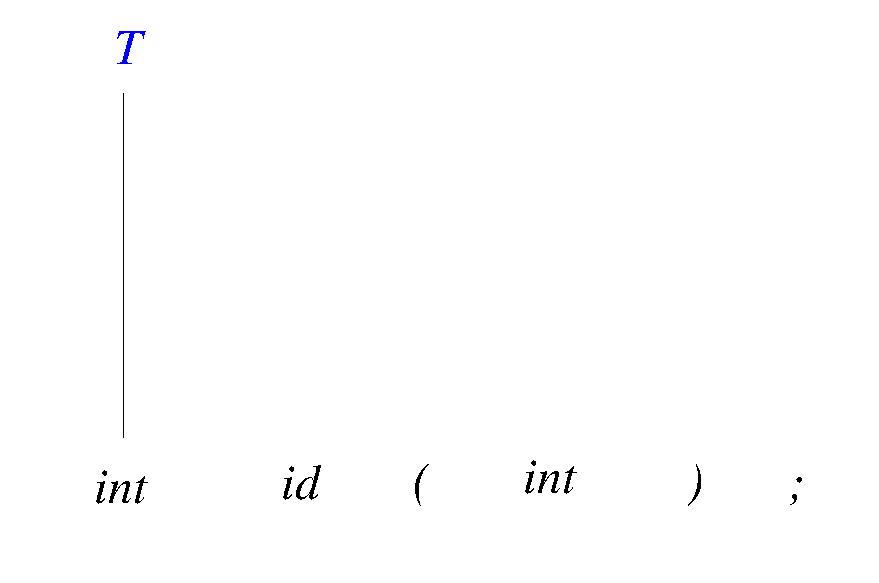
\includegraphics[scale=0.5]{figuras/Cap3/SLR-paso-inicial.pdf} \\ 
        (a) \\ 
        \\
        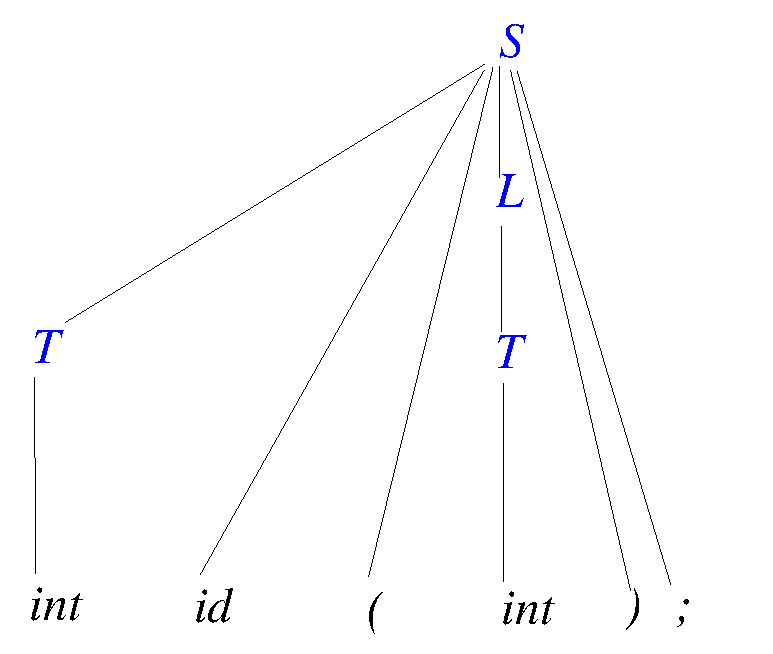
\includegraphics[scale=0.5]{figuras/Cap3/SLR-paso-final.pdf}  \\
        (b)
    \end{tabular}
    \caption{Árbol sintáctico: pasos (a) inicial y (b) final del análisis sintáctico ascendente SLR}\label{fig:pasos-analisis-ascendente-SLR}
\end{figure}

\newpage 

\section{SimAS 1.0}\label{sec:SimAs1.0}

Este Trabajo de Fin de Grado se centra en el desarrollo de un simulador de analizadores sintácticos descendentes, habiendo existido una primera versión previa denominada SimAs 1.0 \cite{vanesa}, la cuál fue posteriormente mejorada. En esta sección, se describen las características principales de dicha versión inicial, la cual servirá como referencia para el desarrollo de la nueva versión.

SimAs 1.0. es una aplicación de escritorio y multiplataforma desarrollada en 2015 con los siguientes recursos de software:
 \begin{itemize}
     \item Sistemas operativos: Ubuntu Linux (versión 12.10) \cite{ubuntu} y Microsoft Windows 7 \cite{windows}.
     \item Lenguaje de programación: Java SE (JDK) 7u40 \cite{java}.
     \item Entorno de desarrollo: NetBeans 7.3.1. \cite{netbeans}.
     \item Biblioteca para la interfaz gráfica: Java Swing \cite{javaswing}.
     \item Biblioteca iText 5.5.0 de Java para la generación de informes en formato pdf \cite{itextpdf}.
     \item XML \cite{xml}: formato utilizado para almacenar las gramáticas formales.
 \end{itemize}

En las siguientes figuras, se describen algunas de las características más importantes del funcionamiento de la versión 1.0 de SimAs. 

 \begin{figure}[!t]
 	\begin{center}
      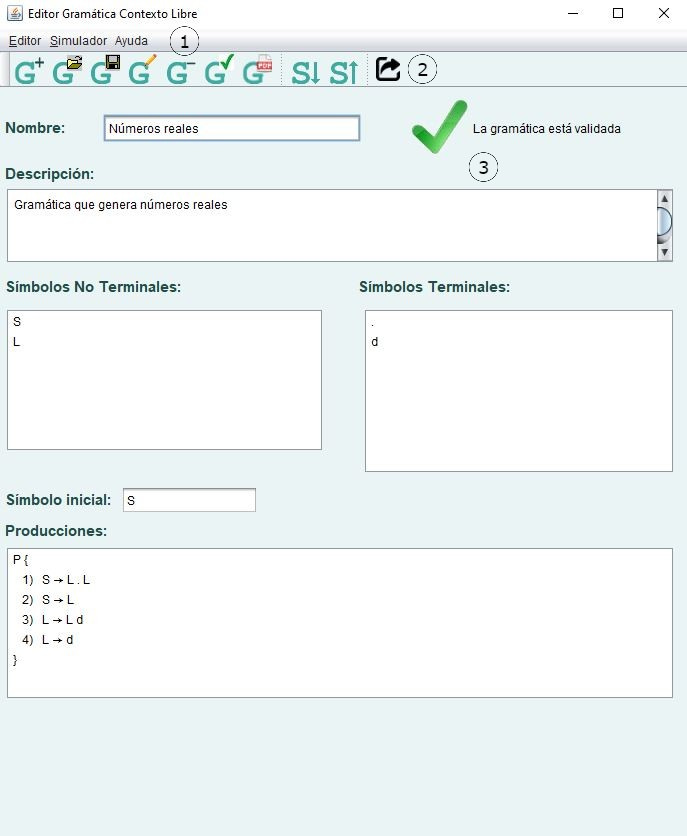
\includegraphics[scale=0.5]{figuras/Cap3/interfaz.JPG} 
       \caption{Interfaz del editor de SimAS 1.0.}\label{fig:SimAS-1.0-editor}
 	\end{center}
 \end{figure}


La figura \ref{fig:SimAS-1.0-editor} muestra la interfaz del editor de SimAS 1.0. En dicha figura, se han numerado algunos componentes que son descritos a continuación:
 \begin{enumerate}
     \item Se muestra la barra de menús donde se puede escoger entre opciones: editor, simulador o ayuda.
     \item La barra de herramientas permite acceder rápidamente a las opciones más frecuentes, como crear abrir o guardar una gramática, verificarla o incluso escoger entre si se prefiere usar el análisis ascendente o descendente.
     \item El editor está compuesto por diferentes formularios para indicar el nombre de la gramática, añadir una pequeña descripción, sus  símbolos terminales y no terminales, establecer el símbolo inicial y definir sus reglas de producción
 \end{enumerate}


 \begin{figure}[!t]
   \begin{center}
      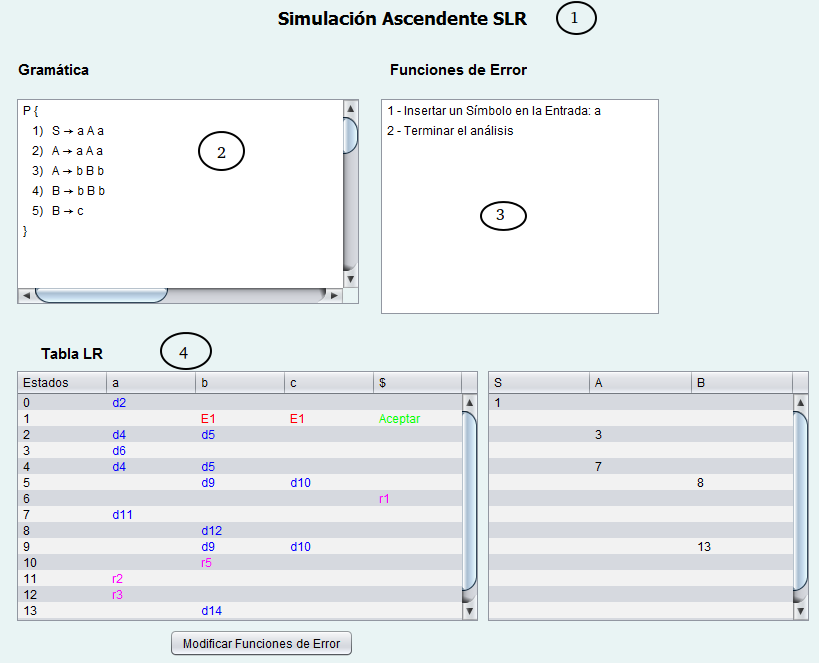
\includegraphics[scale=0.40]{figuras/Cap3/da12.png} 
       \caption{Panel del editor de SimAS 1.0 }\label{fig:SimAS-1.0-editor-funciones-de-error}
 	\end{center}
   \end{figure}

La figura \ref{fig:SimAS-1.0-editor-funciones-de-error} muestra cómo se pueden asignar funciones de tratamiento de errores en el método SLR de análisis sintáctico ascendente. Los componentes numerados se describen a continuación:
\begin{enumerate}
     \item Se indica el tipo de simulación que se llevará a cabo.
     \item Se muestra la gramática de contexto libre que se va a utilizar.
     \item Funciones de tratamiento de errores que se pueden utilizar en  la simulación del análisis sintáctico.
     \item Tabla de análisis LR
\end{enumerate}

\begin{figure}[!t]
 	\begin{center}
      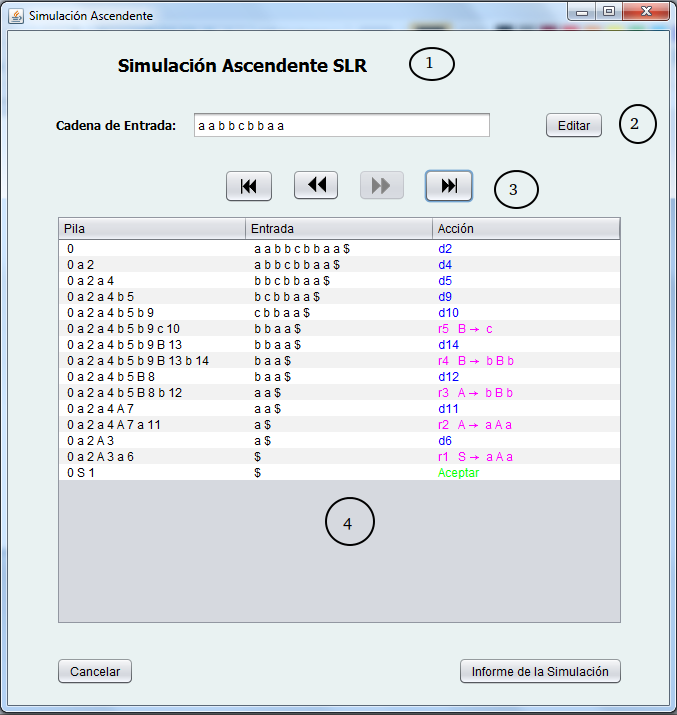
\includegraphics[scale=0.40]{figuras/Cap3/da14.png} 
       \caption{Ventana del simulador de SimAS 1.0.}\label{fig:SimAS-1.0-simulador}
 	\end{center}
\end{figure}

Por último, la figura \ref{fig:SimAS-1.0-simulador} muestra la ventana para la simulación del método SLR de análisis sintáctico ascendente:
\begin{enumerate}
     \item Se indica el tipo de simulación que se va a realizar: simulación ascendente SLR.
     \item Formulario para introducir y editar una cadena de entrada para poder realizar la simulación.
     \item Se muestran una serie de flechas que permiten reproducir la simulación hacia adelante, hacia atrás, etc.
     \item En este último apartado, se muestran los resultados de la simulación.
\end{enumerate}


\section{SimAS 2.0}\label{sec:SimAs2.0}

SimAS 2.0 \cite{juan} se desarrolló para corregir y ampliar la versión de SimAS 1.0 \cite{vanesa}. SimAS 1.0 se instaló en diferentes equipos y se comprobó que permitía simular el funcionamiento de los analizadores sintácticos descendentes y ascendentes. Sin embargo, se detectaron algunos fallos y limitaciones que se intentaron corregir con mejoras que se enumeran a continuación:
\begin{enumerate}
     \item Mejorar el almacenamiento de las gramáticas de contexto libre en formato XML. 
         \begin{itemize}
         \item Procesar de forma individualizada los símbolos de la parte derecha de una regla de producción.
         \item Al cargar una gramática, respetar el orden de sus reglas de producción. No se respeta si ya hay otra gramática previamente cargada.
         \end{itemize}
     \item Validar la gramática cuando se cargue o se modifique, es decir, comprobar que no tiene símbolos y reglas inútiles. En la versión anterior, se debía pulsar un botón para validar.
     \item Al eliminar la recursividad por la izquierda o factorizar por la izquierda, permitir que se pueda conservar la gramática original y la nueva gramática. Además, también debe permitir la enumeración de las reglas de producción de la nueva gramática.
     \item Permitir que la gramática que se está procesando se pueda mostrar o consultar en cualquier momento de forma simultánea en cualquier paso del proceso de simulación de los analizadores sintácticos.
     \item Al construir los conjuntos Primero y Siguiente, mostrar las dependencias entre los conjuntos.
     \item Simular correctamente las gramáticas con reglas épsilon. En particular, calcular correctamente el conjunto Primero en gramáticas reglas épsilon.
     \item Crear funciones predefinidas de recuperación de errores en las simulaciones de los analizadores sintácticos. 
     \item Permitir que se puedan completar las celdas vacías de la tabla de análisis sintáctico descendente con reglas épsilon, cuando proceda, sin tener que predefinir funciones de error.
     \item Permitir que se puedan completar las celdas vacías de la tabla de análisis sintáctico ascendente con reducciones, cuando proceda, sin tener que predefinir funciones de error.
     \item Mostrar las derivaciones obtenidas por los analizadores sintácticos.
     \item Permitir la generación de informes en formato pdf. La aplicación SimAS podía generar estos informes, pero la actualización del sistema operativo no lo permite ahora.
\end{enumerate}

Además, se intentó que la nueva versión  SimAS 2.0 permitiese la generación ``paso a paso'' de los árboles sintácticos de las derivaciones generadas al simular los analizadores sintácticos descendentes o ascendentes.


En su momento, se consideró que el desarrollo de la versión 2.0 estaba justificado por las siguientes razones:
\begin{itemize}
     \item La nueva versión del simulador SimAS 2.0 sería de gran ayuda para que los estudiantes pudiesen aprender ``paso a paso'' el funcionamiento de los analizadores sintácticos descendentes y ascendentes.
     \item La corrección de los errores de SimAS 1.0 evitará que los estudiantes puedan cometerlos.
     \item La inclusión de la generación de los árboles sintácticos asociados a las derivaciones permitiría que los estudiantes comprendan mejor el funcionamiento de los analizadores sintácticos.
\end{itemize}

En las siguientes figuras, se describen algunas de las características más importantes del funcionamiento de la versión 2.0 de SimAS.
 
\begin{figure}[p]
 	\begin{center}
      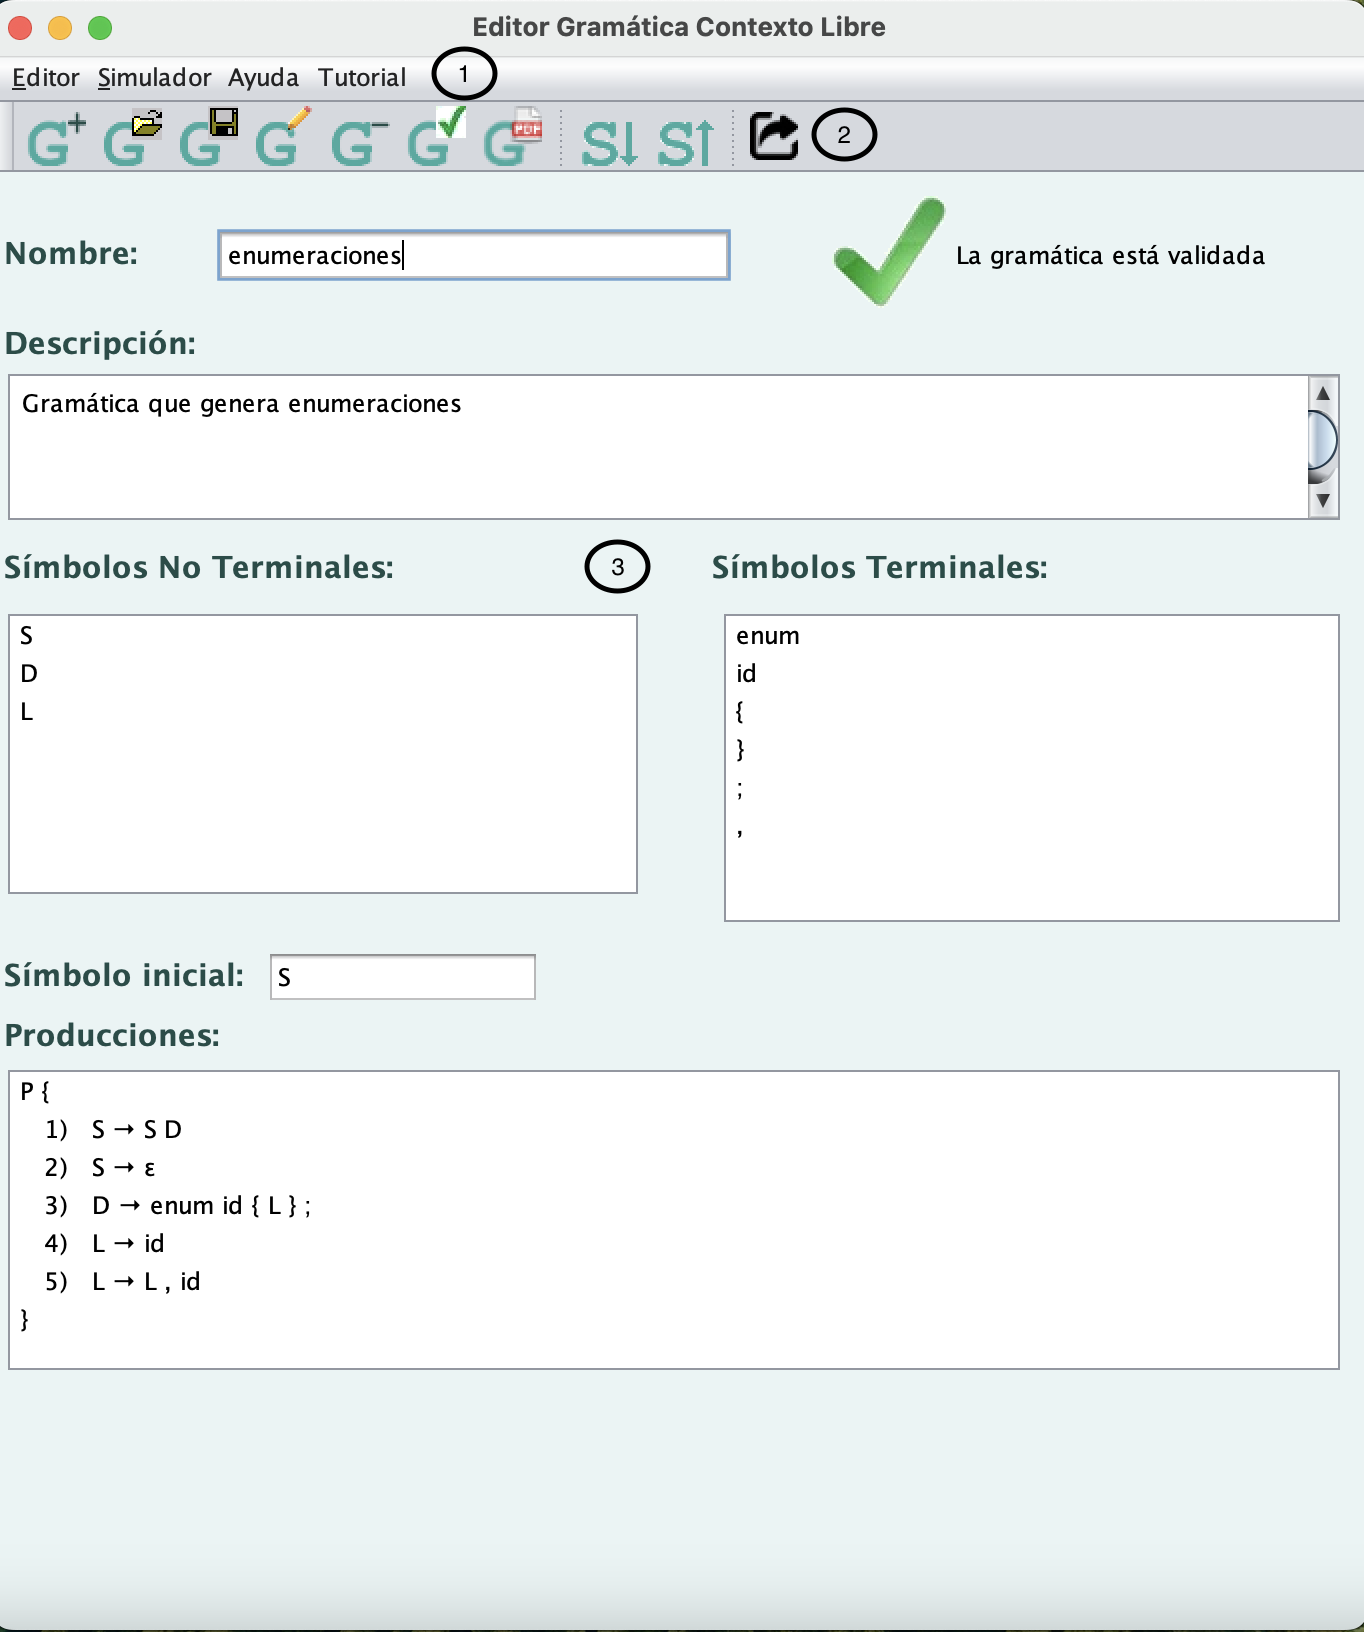
\includegraphics[scale=0.5]{figuras/Cap3/SimAS2/editor.png} 
       \caption{Interfaz del editor de SimAS 2.0.}\label{fig:SimAS-2.0-editor}
 	\end{center}
\end{figure}


La figura \ref{fig:SimAS-2.0-editor} muestra la interfaz del editor de SimAS 2.0, la cual contiene pocas variaciones respecto a la versión original. En dicha figura, se han numerado algunos componentes que son descritos a continuación:
 \begin{enumerate}
     \item La interfaz presenta una barra de menús que brinda opciones como editor, simulador, ayuda y un tutorial detallado para comprender su funcionamiento.
     \item Además, la barra de herramientas facilita el acceso a las funciones más utilizadas, como la creación, apertura y guardado de gramáticas, así como la verificación de las mismas. También permite elegir entre el análisis ascendente y el descendente.
     \item En cuanto al editor, se compone de distintos formularios que permiten especificar el nombre de la gramática, agregar una breve descripción, definir los símbolos terminales y no terminales, establecer el símbolo inicial y definir las reglas de producción.
 \end{enumerate}

\begin{figure}[p]
 	\begin{center}
      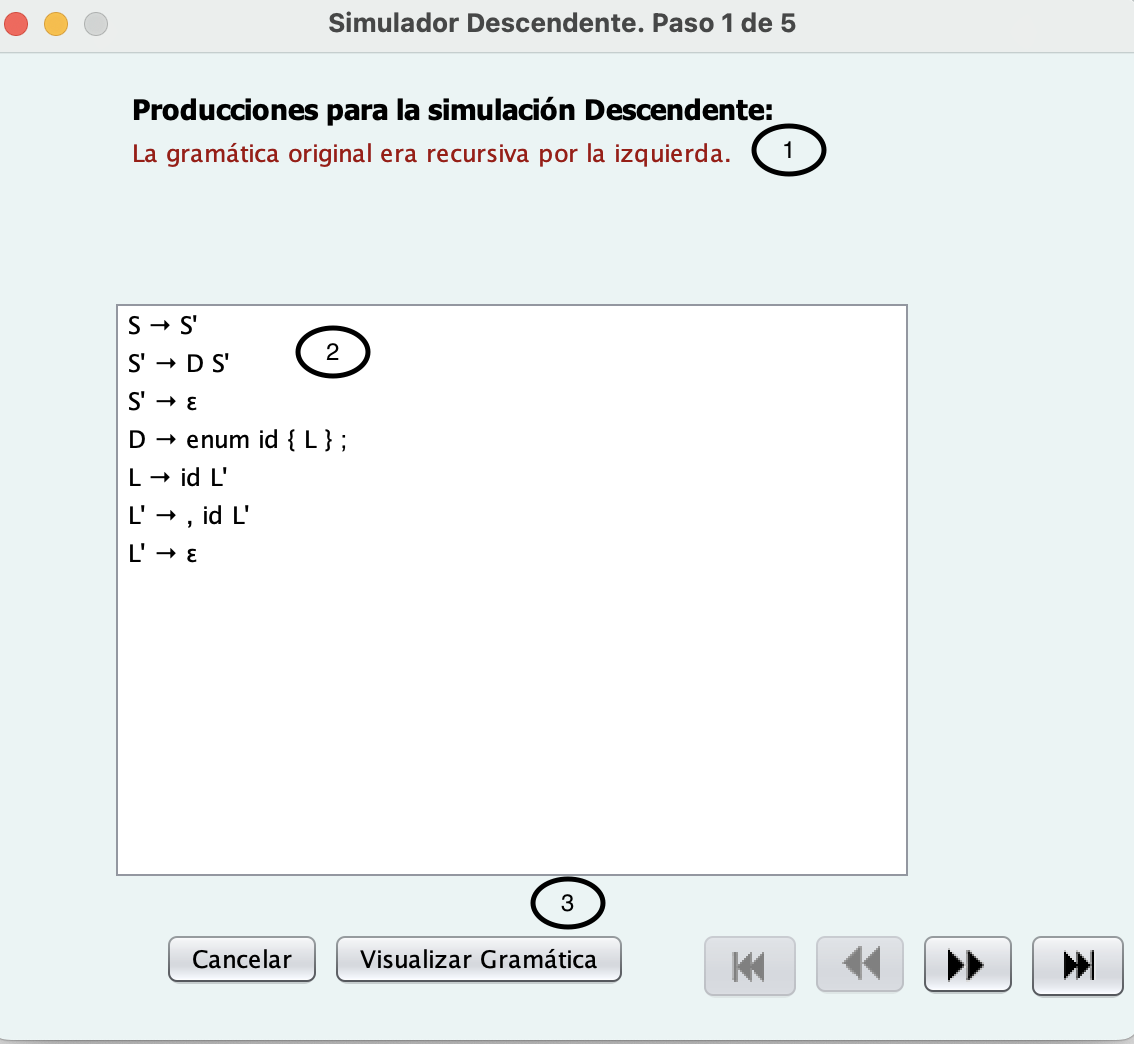
\includegraphics[scale=0.5]{figuras/Cap3/SimAS2/paso1.png} 
       \caption{Corrección de gramáticas de SimAS 2.0.}\label{fig:SimAS-2.0-paso1}
 	\end{center}
\end{figure}


La figura \ref{fig:SimAS-2.0-paso1} muestra el primer paso a realizar para el análisis de gramáticas en SimAS 2.0, que consiste en la eliminación de recursividad de la gramática original. En dicha figura, se han numerado algunos componentes que son descritos a continuación:
 \begin{enumerate}
     \item En primer lugar, aparece un mensaje indicativo con los cambios realizados a la gramática original.
     \item En segundo lugar, se muestra la nueva gramática generada tras realizar los cambios oportunos a la gramática original.
     \item Además, nos da la opción de consultar la gramática original para poder comparar ambas gramáticas.
 \end{enumerate}

 \begin{figure}[p]
 	\begin{center}
      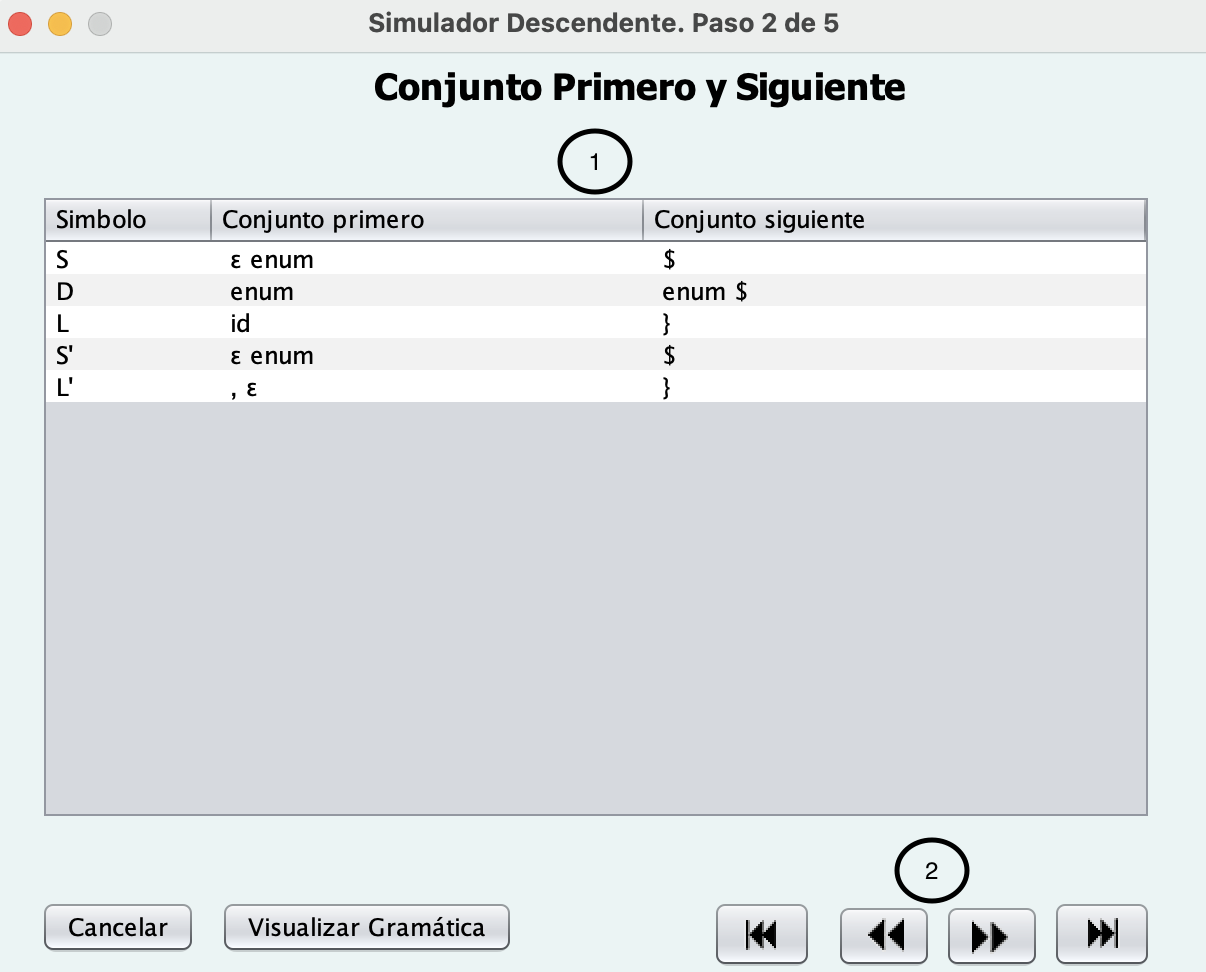
\includegraphics[scale=0.5]{figuras/Cap3/SimAS2/paso2.png} 
       \caption{Conjunto Primero y Siguiente de SimAS 2.0.}\label{fig:SimAS-2.0-paso2}
 	\end{center}
\end{figure}

\newpage
La figura \ref{fig:SimAS-2.0-paso2} muestra los conjuntos Primero y Siguiente generados para el análisis de gramáticas en SimAS 2.0. En dicha figura, se han numerado algunos componentes que son descritos a continuación:
 \begin{enumerate}
     \item El usuario puede ver una tabla con los conjuntos Primero y Siguiente correspondientes a cada símbolo no terminal.
     \item También tenemos un menú común a todos los pasos, que anteriormente no se había mencionado, que permite avanzar paso a paso o  avanzar directamente al último paso.
 \end{enumerate}

\begin{figure}[htp]
 	\begin{center}
      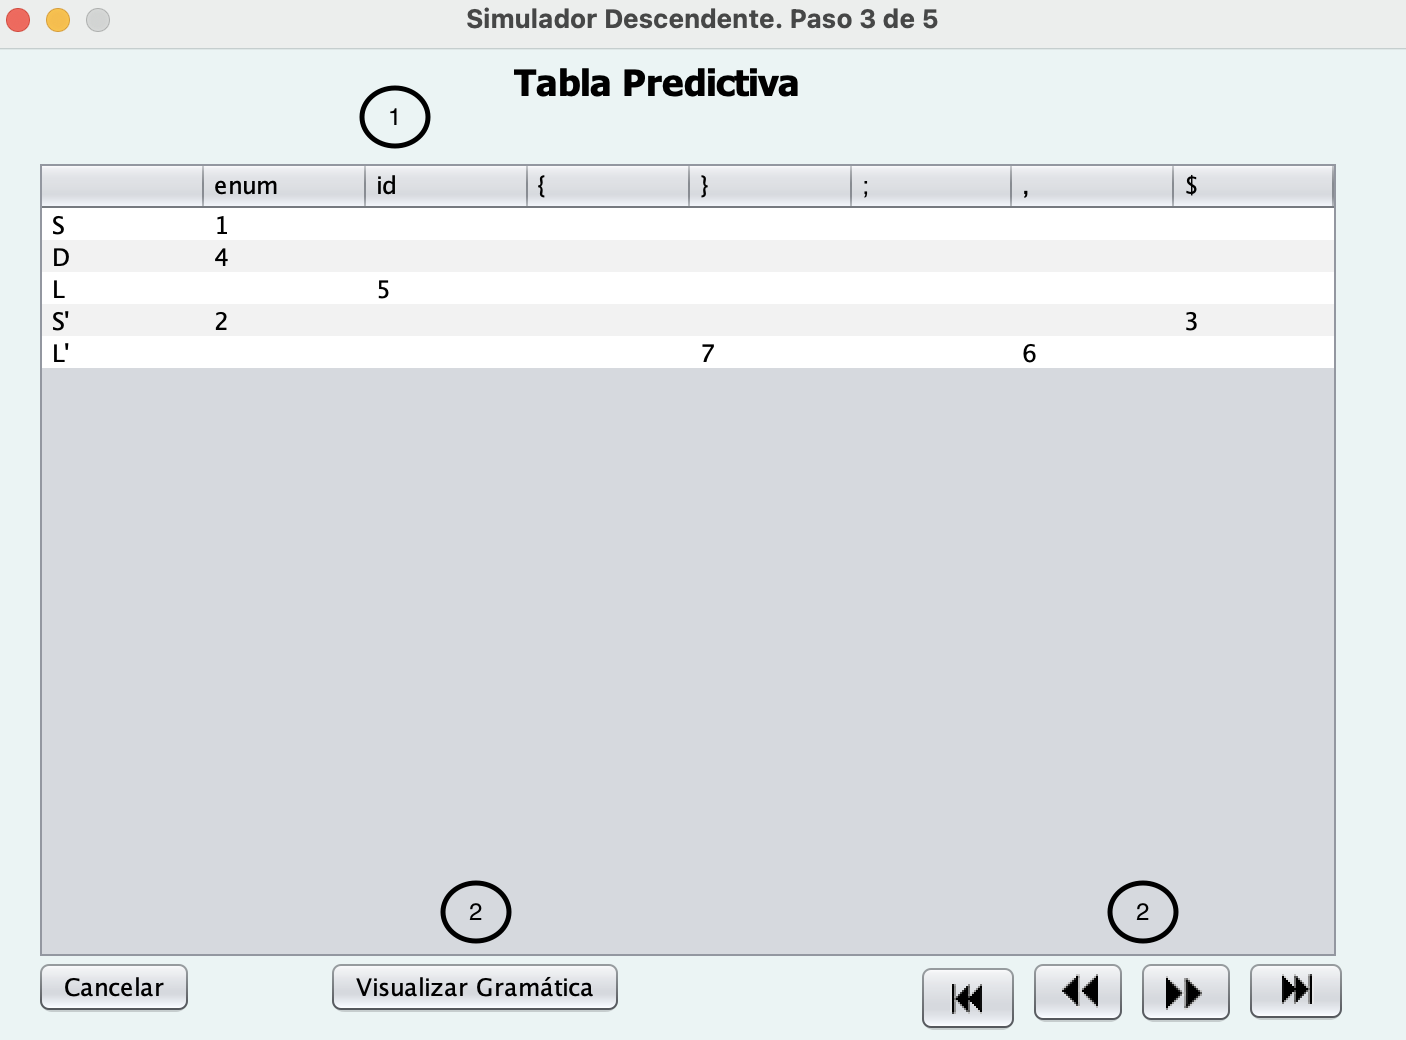
\includegraphics[scale=0.5]{figuras/Cap3/SimAS2/paso3.png} 
       \caption{Tabla predictiva de SimAS 2.0.}\label{fig:SimAS-2.0-paso3}
 	\end{center}
\end{figure}

La figura \ref{fig:SimAS-2.0-paso3} muestra la tabla predictiva generada por el análisis de gramáticas en SimAS 2.0. En dicha figura, se han numerado algunos componentes que son descritos a continuación:
 \begin{enumerate}
     \item En primer lugar, la interfaz contiene la tabla predictiva generada por el programa para la gramática.
     \item Al igual que en el resto de pasos intermedios, el programa contiene la posibilidad de visualizar la gramática original, y el menú de avance y retroceso.
 \end{enumerate}

 \begin{figure}[htp]
 	\begin{center}
      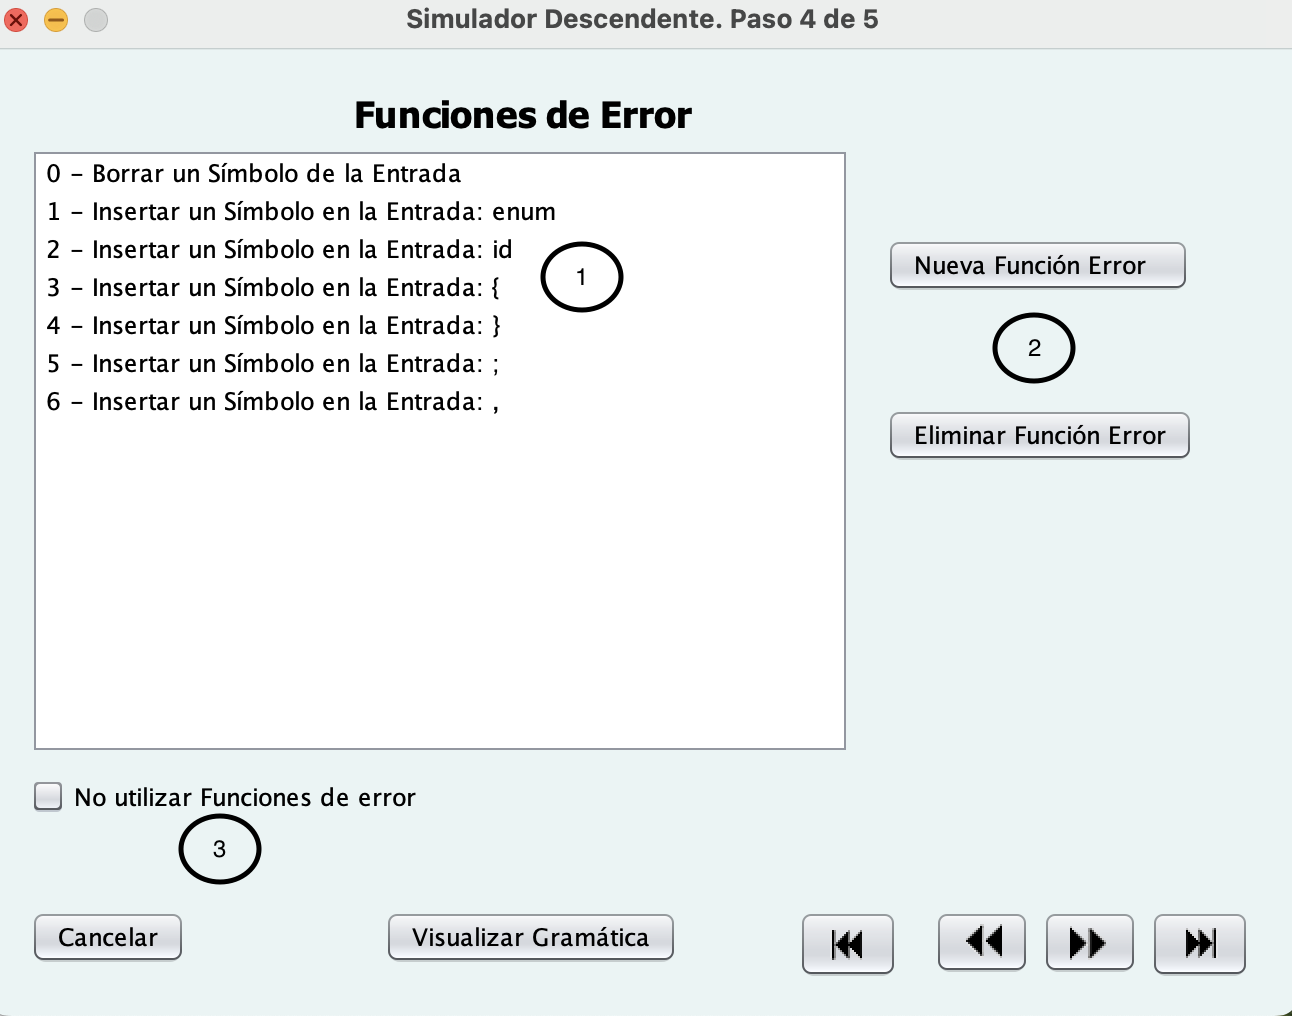
\includegraphics[scale=0.5]{figuras/Cap3/SimAS2/paso4.png} 
       \caption{Tabla predictiva de SimAS 2.0.}\label{fig:SimAS-2.0-paso4}
 	\end{center}
\end{figure}

La figura \ref{fig:SimAS-2.0-paso4} muestra las funciones de error predefinidas o que podemos definir respecto para las gramáticas en SimAS 2.0. En dicha figura, se han numerado algunos componentes que son descritos a continuación:
 \begin{enumerate}
     \item En primer lugar, podemos ver las gramáticas predefinidas que contiene el programa, que comparando con la versión anterior, vemos que son muchas más.
     \item Además, un cambio importante respecto a la versión anterior, es que ésta da la posibilidad de añadir o eliminar funciones de error directamente desde esta interfaz.
     \item Otro cambio significativo respecto a la versión anterior es que se da la opción de no usar funciones de error, lo que hace que el programa salte directamente a la parte final, sin pasar por el paso 5.
 \end{enumerate}

\begin{figure}[htp]
 	\begin{center}
      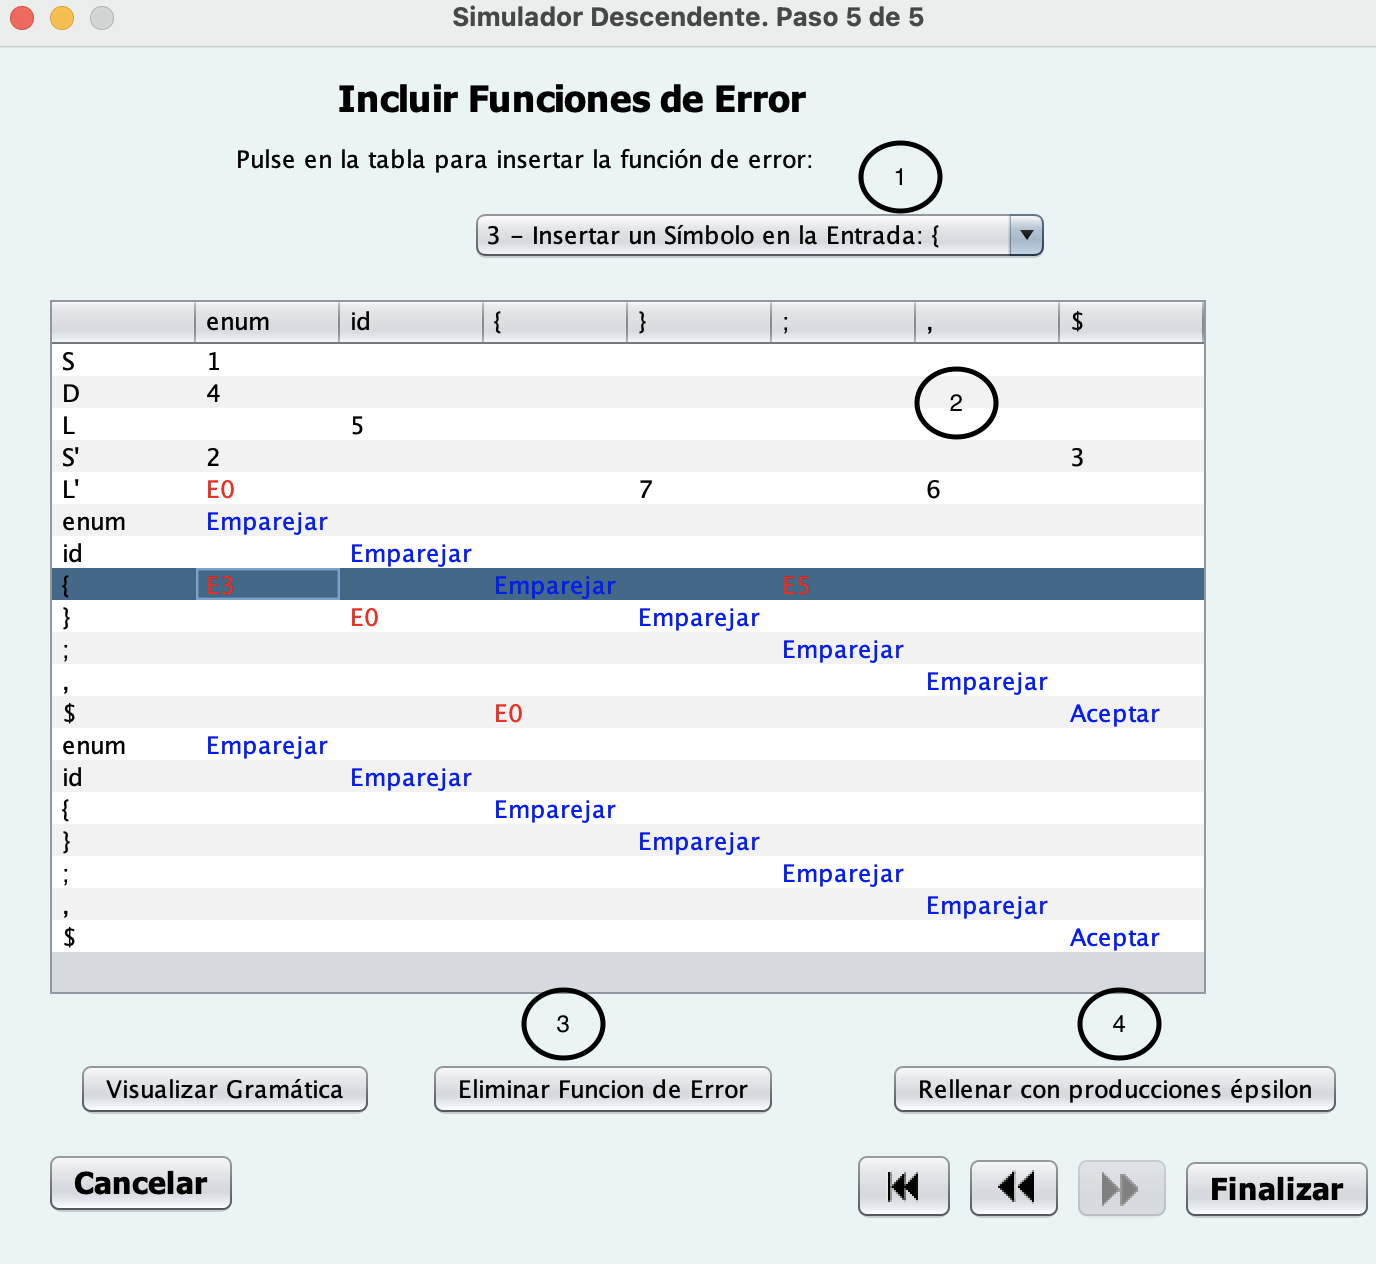
\includegraphics[scale=0.5]{figuras/Cap3/SimAS2/paso5.png} 
       \caption{Tabla predictiva con funciones de errores de SimAS 2.0.}\label{fig:SimAS-2.0-paso5}
 	\end{center}
\end{figure}

La figura \ref{fig:SimAS-2.0-paso5} muestra las funciones de error predefinidas o que podemos definir respecto para las gramáticas en SimAS 2.0. En dicha figura, se han numerado algunos componentes que son descritos a continuación:
 \begin{enumerate}
     \item En primer lugar, se ofrece un menú con las funciones de error definidas en el paso anterior.
     \item En segundo lugar, se tiene la tabla predictiva aumentada para que el usuario añada dichas funcionas de forma intuitiva y muy rápida.
     \item Se añade la opción de eliminar alguna función de error que el usuario estime como incorrecta.
     \item Finalmente, el programa da la opción de rellenar la tabla con las producciones épsilon que pertenezcan a dicha gramática.
 \end{enumerate}

\begin{figure}[htp]
 	\begin{center}
      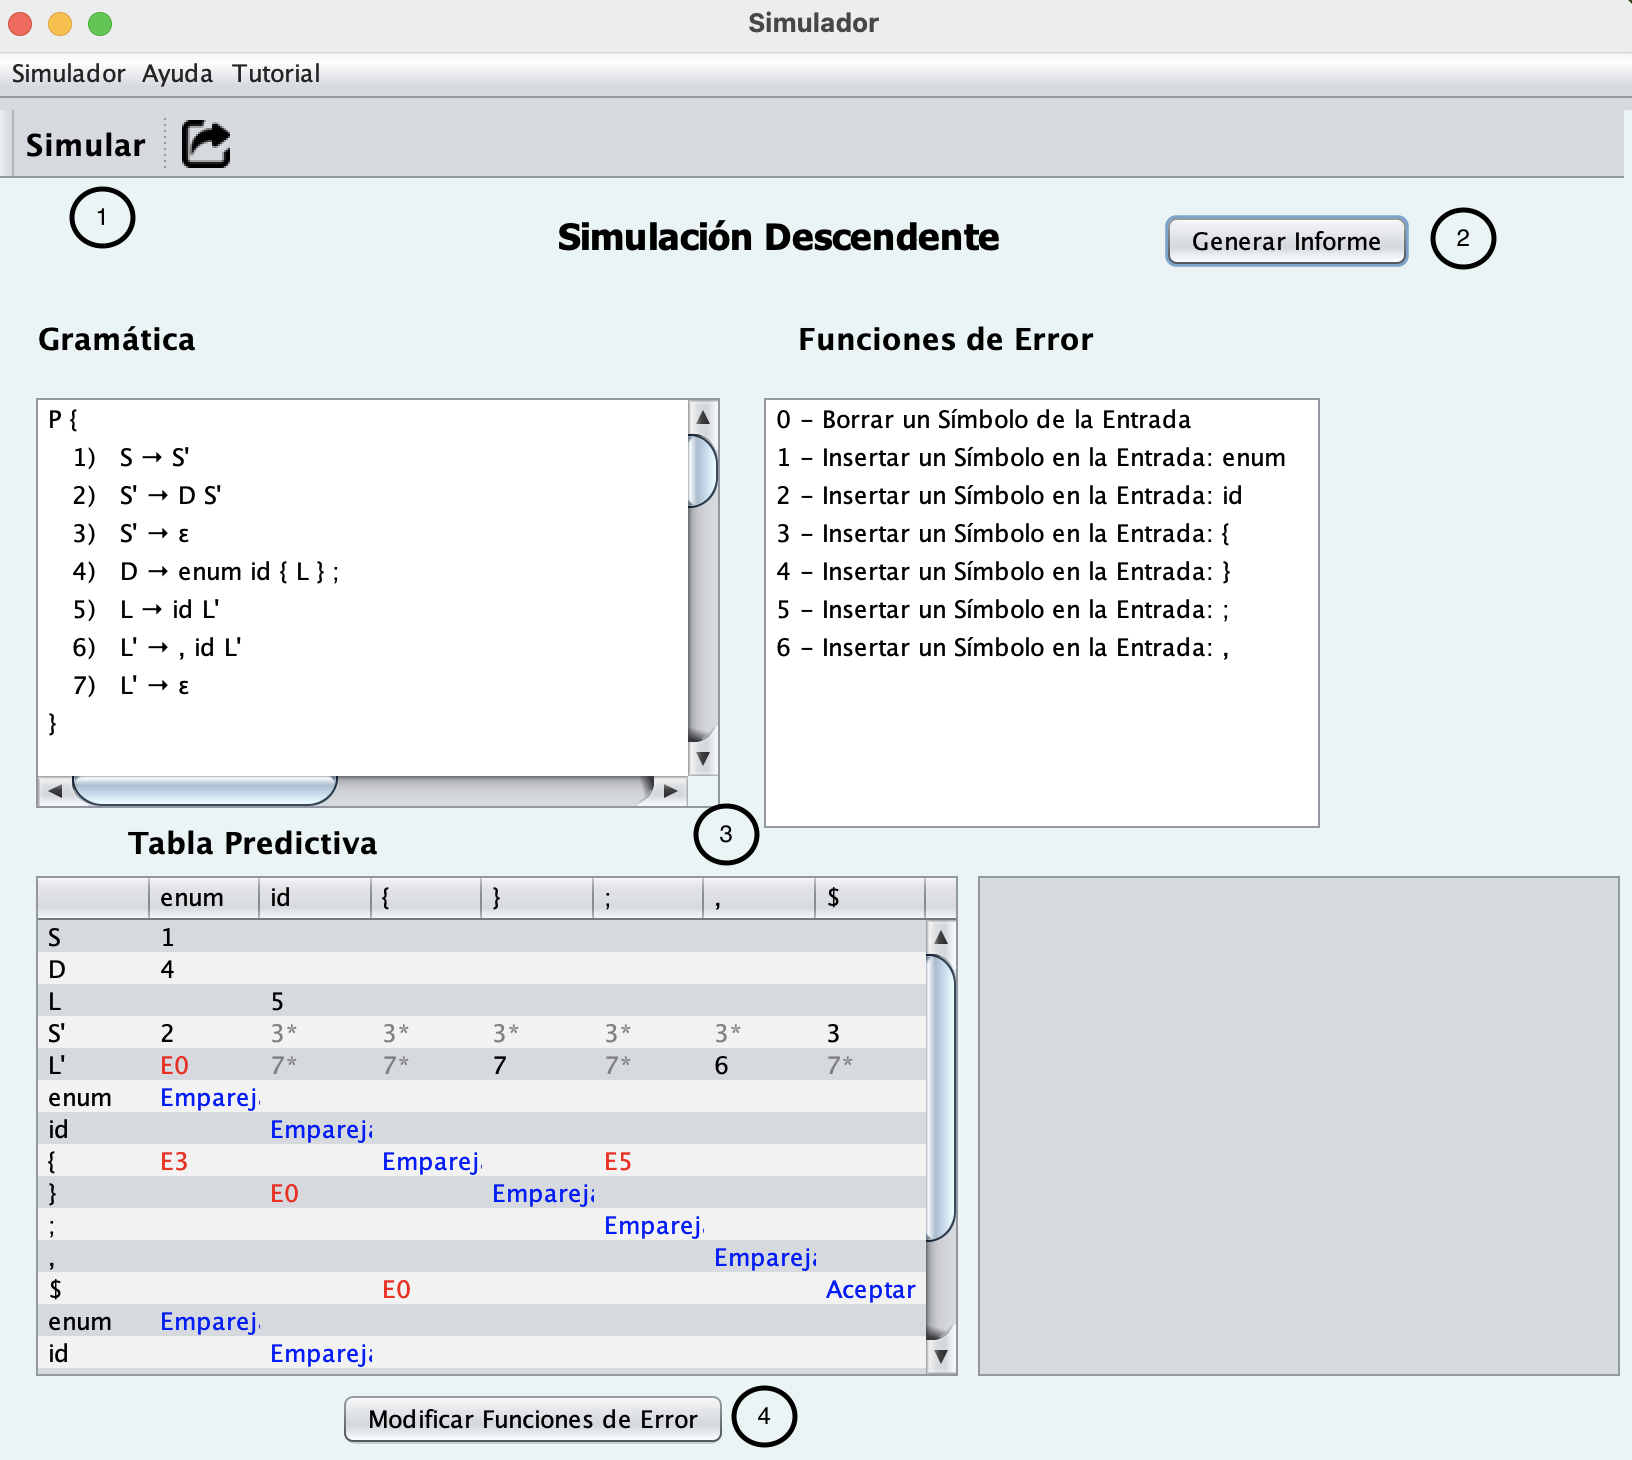
\includegraphics[scale=0.5]{figuras/Cap3/SimAS2/finalizar.png} 
       \caption{Tabla predictiva con funciones de errores de SimAS 2.0.}\label{fig:SimAS-2.0-finalizar}
 	\end{center}
\end{figure}

\newpage
La figura \ref{fig:SimAS-2.0-finalizar} muestra todo lo obtenido anteriormente respecto al análisis de las gramáticas en SimAS 2.0. En dicha figura, se han numerado algunos componentes que son descritos a continuación:
 \begin{enumerate}
     \item En primer lugar, nos da la posibilidad de realizar una simulación introduciendo algunos elementos de la gramática.
     \item En segundo lugar, se ofrece la posibilidad de generar un informe con todos los datos obtenidos en el análisis de la gramática.
     \item A continuación, se muestra un resumen con toda la información obtenida hasta el momento, como lo es la gramática sin recursividad, las funciones de error usadas y la tabla predictiva ya completa.
     \item Además, se tiene la opción de modificar las funciones de error que se han elegido con anterioridad.
 \end{enumerate}


\subsection{Fallos generales identificados en SimAS 2.0}

Durante el análisis y uso de la aplicación SimAS 2.0, se han identificado varios fallos y limitaciones que afectan a su funcionamiento y su utilidad como herramienta didáctica. A continuación, se detallan los fallos más relevantes:

\begin{enumerate}
    \item \textbf{Problemas en la persistencia de gramáticas:} al crear o modificar gramáticas en SimAS 2.0, se han observado ocasiones en las que los cambios realizados no se guardan correctamente en el sistema. Esto puede resultar en la pérdida de datos y en la necesidad de rehacer el trabajo. Por otro lado, cuando las gramáticas se guardan correctamente, la interpretación de los símbolos epsilon no se realiza de manera adecuada en algunos casos, lo que puede generar confusiones y errores en el análisis sintáctico.

    \item \textbf{Limitación en la generación de informes:} la funcionalidad de generación de informes presenta una limitación significativa, ya que solo se realiza correctamente en sistemas operativos Windows. En otros sistemas operativos, como Linux o macOS, la generación de informes puede fallar, lo que afecta la portabilidad y la usabilidad de la aplicación.
    
    \item \textbf{Problemas al añadir errores:} se ha observado que, en ciertas situaciones, al intentar agregar errores, la aplicación no permite su inserción en la parte de la tabla correspondiente, normalmente en la parte inferior. Este problema afecta la capacidad de los usuarios para simular y corregir errores sintácticos en gramáticas definidas.
    
    \item \textbf{Complejidad en la gestión de producciones gramaticales:} la gestión de producciones gramaticales, como añadir, modificar o eliminar producciones, presenta una complejidad innecesaria. Los usuarios encuentran dificultades al realizar estas operaciones, lo que afecta la eficiencia y la experiencia de uso de la aplicación.
    
    \item \textbf{Error ocasional en la generación de conjuntos Primero y Siguiente:} se han observado fallos intermitentes en el proceso de generación de conjuntos Primero y Siguiente. Estos conjuntos son fundamentales para varios algoritmos de análisis sintáctico, por lo que los errores en su cálculo pueden afectar a la precisión y la fiabilidad de la simulación.
    
    \item \textbf{Generación parcial de árboles de análisis:} actualmente, SimAS 2.0 no cuenta con la capacidad total de generar árboles sintácticos que representen las derivaciones realizadas durante el análisis sintáctico. El programa genera correctamente los árboles descendentes, excepto los nodos con el símbolo épsilon, y parcialmente los ascendentes en el sistema operativo Windows, pero, en otros sistemas operativos, no los genera bien. Esta funcionalidad es crucial para la comprensión visual del proceso de análisis y su ausencia limita el potencial educativo de la aplicación.
\end{enumerate}

La corrección y mejora de estos fallos son aspectos prioritarios para garantizar el correcto funcionamiento y la utilidad pedagógica de SimAS 2.0 como herramienta de aprendizaje en el ámbito del análisis sintáctico de lenguajes formales.

En la siguientes seccións, se profundizará con más detalle en los fallos encontrados para cada sistema operativo en el que se ha probado, ya que dependiendo de éste, la aplicación actúa de distinta forma.

Se va a utilizar la siguiente gramática de contexto libre para describir los fallos detectados en la apliación SimAS 2.0:
\begin{align*}
P = \{ & \\ 
S &\rightarrow S \, D \\
S &\rightarrow \varepsilon \\
D &\rightarrow T \, L \, ; \\
T &\rightarrow \text{REAL} \\
T &\rightarrow \text{ENTERO} \\
L &\rightarrow L \, , \, \text{ID} \\
L &\rightarrow \text{ID} \\
  & \}
\end{align*}

Esta es una gramática que genera declaraciones de variables tipo entero y real.

\subsection{Fallos encontrados en Windows}
Durante las pruebas realizadas en el sistema operativo Windows 11, se han identificado varios fallos en el funcionamiento de la aplicación SimAS. Uno de los problemas más destacados se refiere a la modificación de la gramática, tanto en los símbolos no terminales como en los símbolos terminales. Los usuarios encuentran dificultades al realizar operaciones como quitar o poner símbolos, así como al intentar renombrar un símbolo.

Además, se observaron inconsistencias en la validación de la gramática, lo que puede llevar a errores en la definición de la misma. Otro problema identificado está relacionado con la funcionalidad de guardar la gramática en el directorio correspondiente. En algunas ocasiones, la gramática no se guarda correctamente, lo que puede resultar en la pérdida de datos importantes para el usuario.

Durante las pruebas, también se identificaron fallos en la generación de los conjuntos Primero y Siguiente, que no se calculan de manera precisa. Esto puede afectar a la precisión de los análisis sintácticos realizados con la aplicación.

Además de los problemas mencionados anteriormente, se han detectado errores relacionados con la paginación del informe generado por la aplicación. La generación del árbol sintáctico para el símbolo épsilon también presenta problemas en algunas situaciones específicas.

Por último, se observó que al volver a acceder a la aplicación después de salir de la simulación descendente, los datos de la simulación anterior persisten de manera inesperada. Esto puede causar confusiones al usuario y afectar a la integridad de los resultados obtenidos.

\subsection{Fallos encontrados en Ubuntu}

En el entorno de Ubuntu 22, se han identificado varios problemas que afectan a la experiencia y funcionalidad de la aplicación SimAS.

Al eliminar un símbolo de la gramática y posteriormente intentar volver a añadirlo, se observa que es necesario cerrar la ventana emergente correspondiente y abrir una nueva para llevar a cabo la acción deseada. Esta situación puede resultar frustrante para el usuario, ya que interrumpe el flujo de trabajo y genera una experiencia poco fluida en la edición de la gramática.

Otro inconveniente detectado radica en el comportamiento al hacer clic repetidamente en la opción ``Visualizar Gramática Original''. En lugar de abrir la ventana una sola vez, se observa que la aplicación abre múltiples instancias de la ventana, lo cual puede resultar confuso para el usuario y generar una sensación de ineficiencia en la navegación por la interfaz, como se puede observar en la imagen \ref{fig:SimAS-2.0-ubuntu1}.

\begin{figure}[htp]
 	\begin{center}
      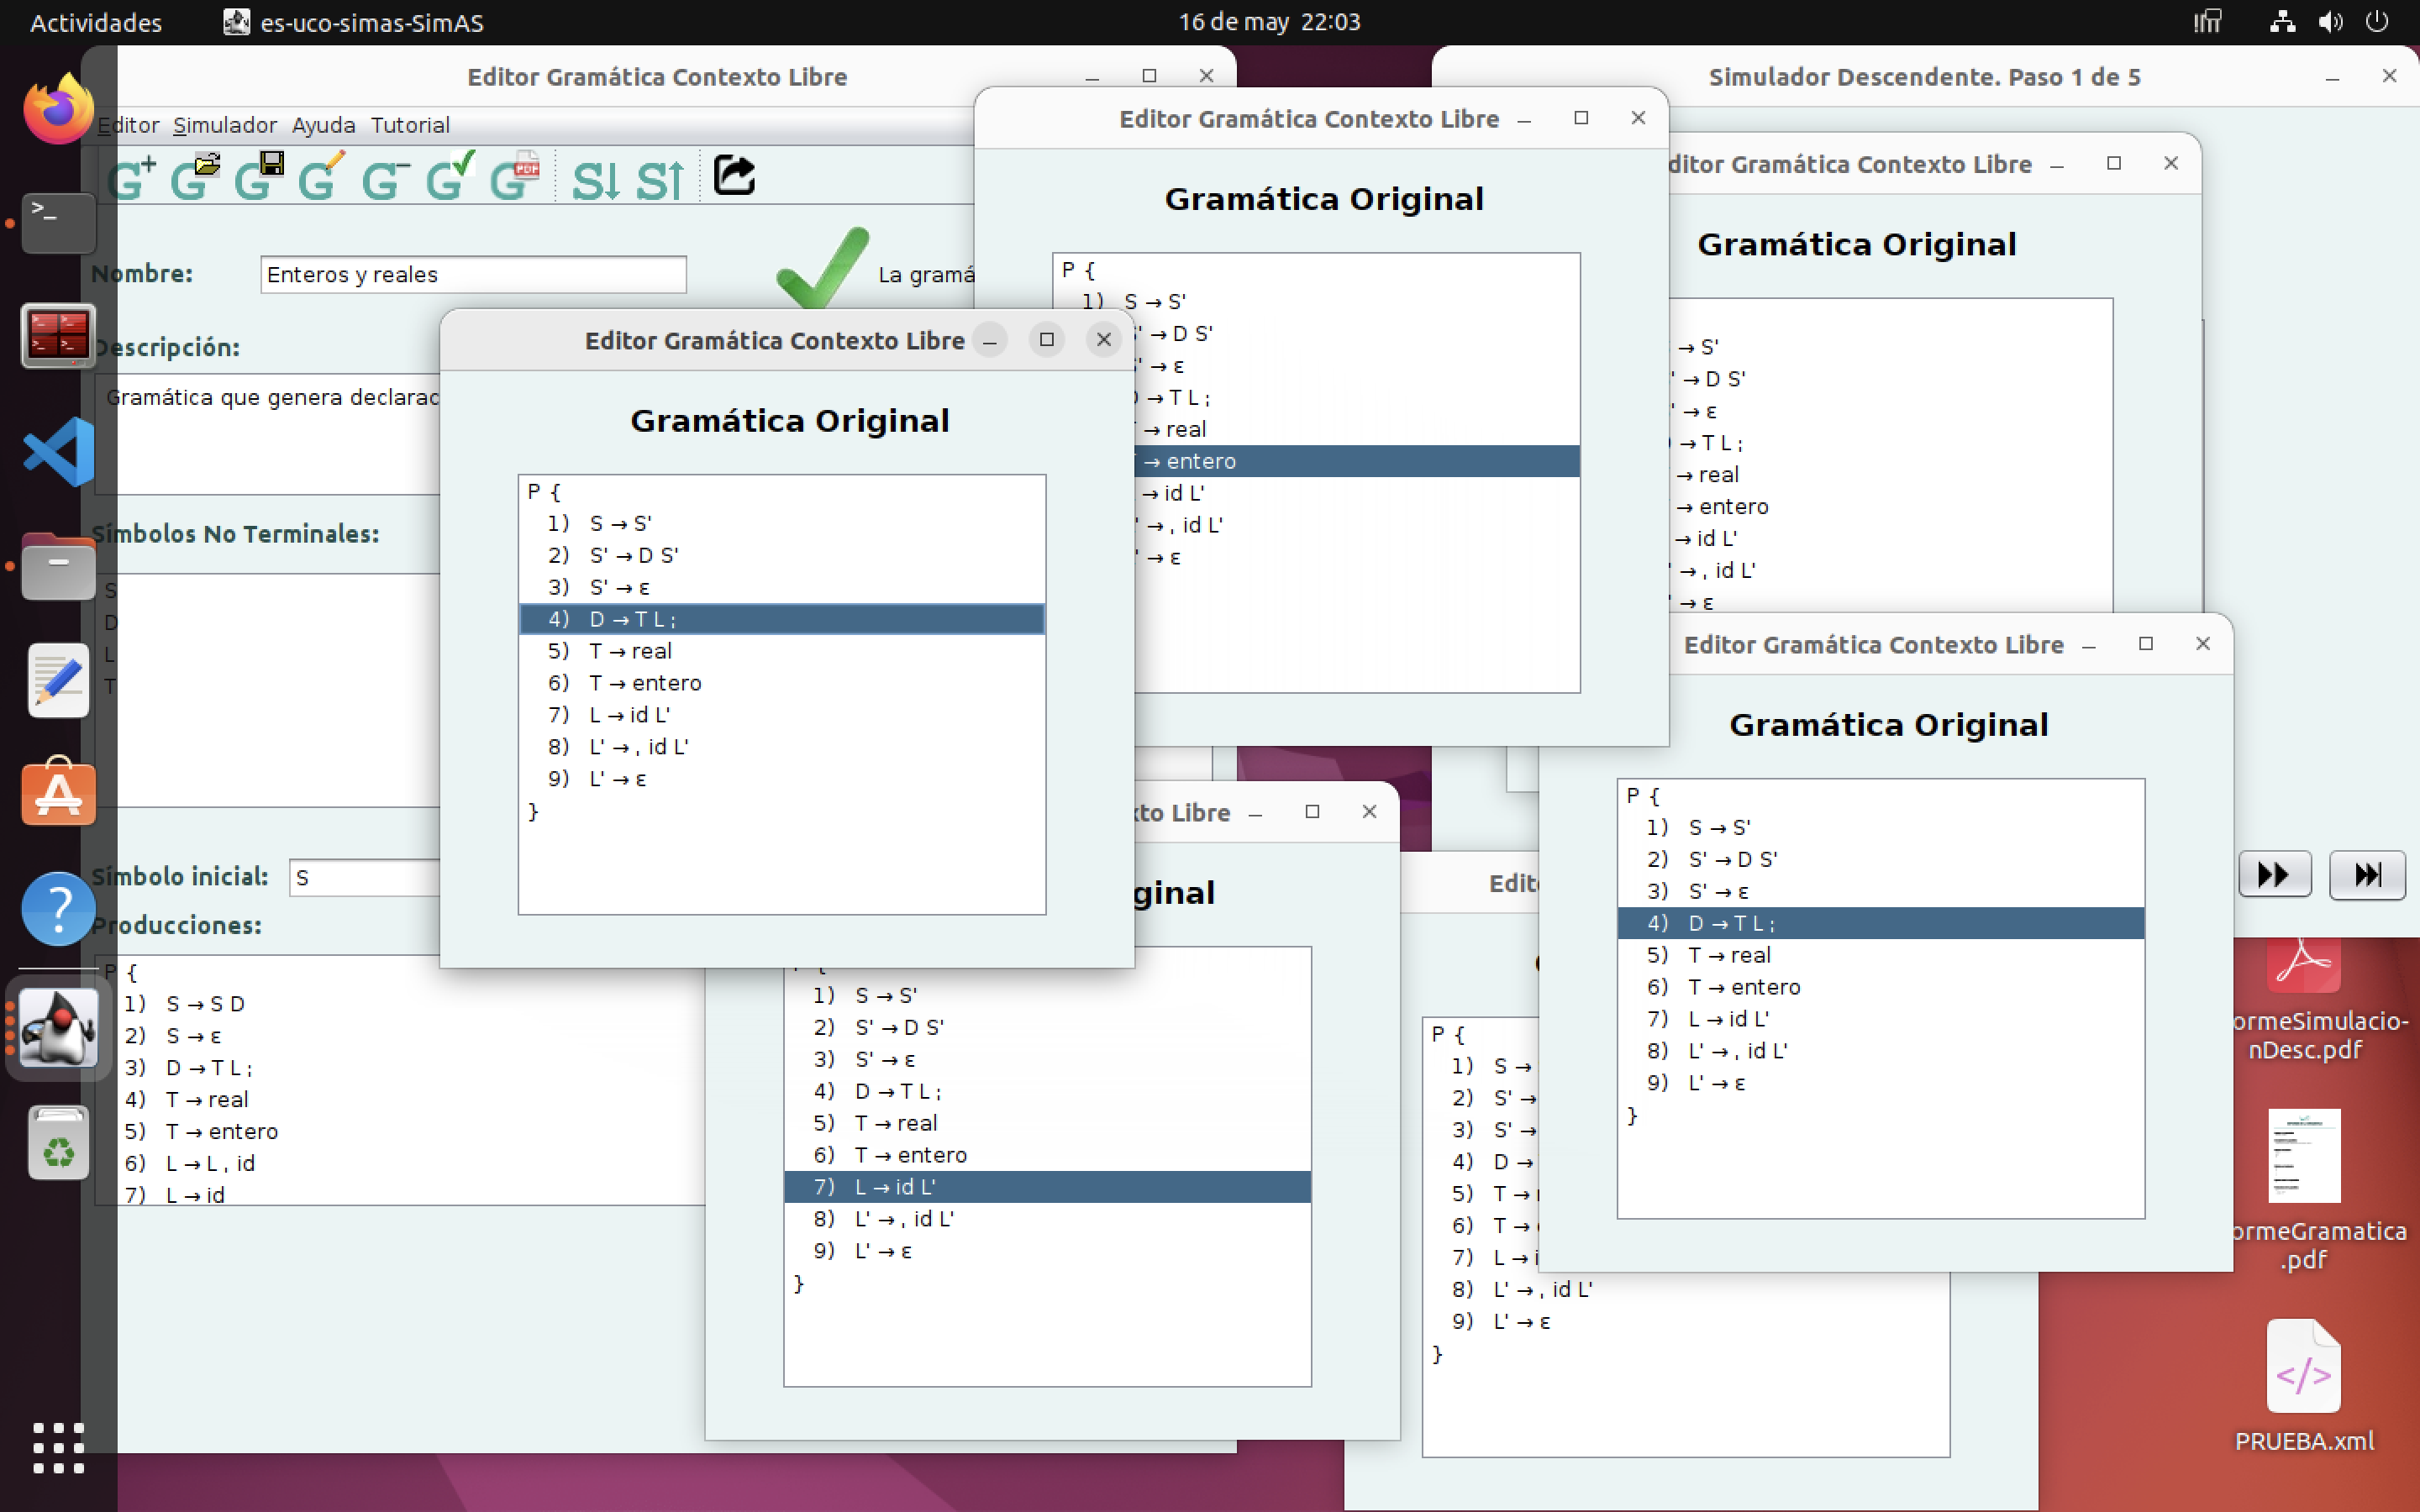
\includegraphics[scale=0.3]{figuras/Cap3/SimAS2/fallos/ubuntu1.png} 
       \caption{Generación repititiva de la visualización de la gramática}\label{fig:SimAS-2.0-ubuntu1}
 	\end{center}
\end{figure}

Además, se ha detectado que la aplicación no enumera las reglas al eliminar la recursividad en la gramática. Esta omisión puede dificultar la identificación y seguimiento de los cambios realizados en la estructura de la gramática, lo que puede conducir a errores o malentendidos durante el proceso de edición.

Otro problema importante afecta a la generación de los conjuntos Primero y Siguiente, los cuales no se calculan correctamente. Estos conjuntos son fundamentales para varios algoritmos de análisis sintáctico, por lo que errores en su cálculo pueden impactar negativamente en la precisión y fiabilidad de la simulación y validación de la gramática.

En relación con las funciones de error, se ha observado que la función de error para terminar el análisis no está predefinida, lo que puede dificultar la gestión de errores durante el análisis sintáctico y generar resultados inesperados.

Asimismo, al añadir una nueva regla de error, la aplicación no asigna automáticamente el siguiente número disponible, lo que puede generar confusiones en la gestión de las reglas de error y dificultar su identificación. En la figura \ref{fig:SimAS-2.0-ubuntu2} se observa la posibilidad de añadir cualquier número a las nuevas funciones de error, sin seguir ningún orden.

\begin{figure}[htp]
 	\begin{center}
      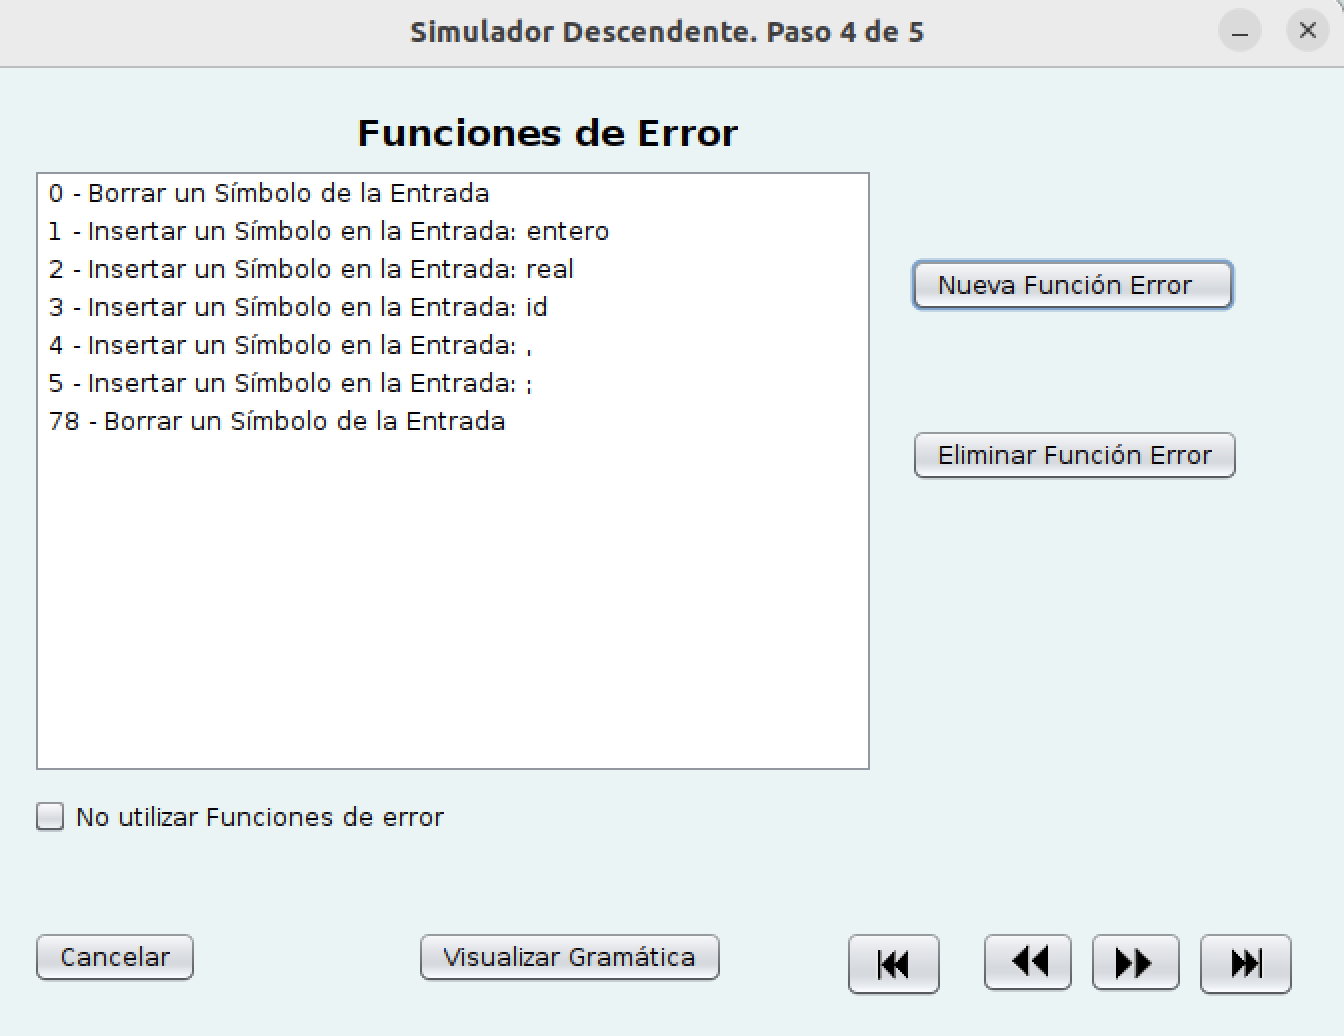
\includegraphics[scale=0.3]{figuras/Cap3/SimAS2/fallos/ubuntu2.png} 
       \caption{Creación de una nueva función de error}\label{fig:SimAS-2.0-ubuntu2}
 	\end{center}
\end{figure}

Otro problema destacable ocurre al intentar modificar las funciones de error después de haber finalizado y regresado al proceso. En esta situación, la aplicación duplica las filas de los símbolos terminales y modifica los estados de la tabla predictiva, lo que puede causar errores en la definición y gestión de las funciones de error.

La generación incorrecta de informes de simulación descendente y la ausencia de generación de informes tras realizar un análisis de una cadena de entrada también se han identificado como fallos significativos en el funcionamiento de la aplicación en el entorno de Ubuntu 22. Estos problemas afectan negativamente a la capacidad del usuario para evaluar y analizar los resultados del análisis sintáctico, lo que impacta en la utilidad y fiabilidad de la aplicación en este sistema operativo.

\subsection{Fallos encontrados en MacOS}

Al crear una nueva gramática, el programa no proporciona una opción para regresar al menú principal, lo que dificulta la navegación dentro de la aplicación. Además, al validar una gramática, se abren dos ventanas emergentes, una con la gramática validada y otra que queda congelada, lo que puede resultar confuso para el usuario, observable en la figura \ref{fig:SimAS-2.0-macos1}. Por otro lado, al intentar copiar y pegar texto al agregar o modificar símbolos de la gramática, así como al cambiar el nombre de los símbolos, la funcionalidad no está habilitada, lo que limita la capacidad del usuario para editar la gramática de manera eficiente.

\begin{figure}[htp]
 	\begin{center}
      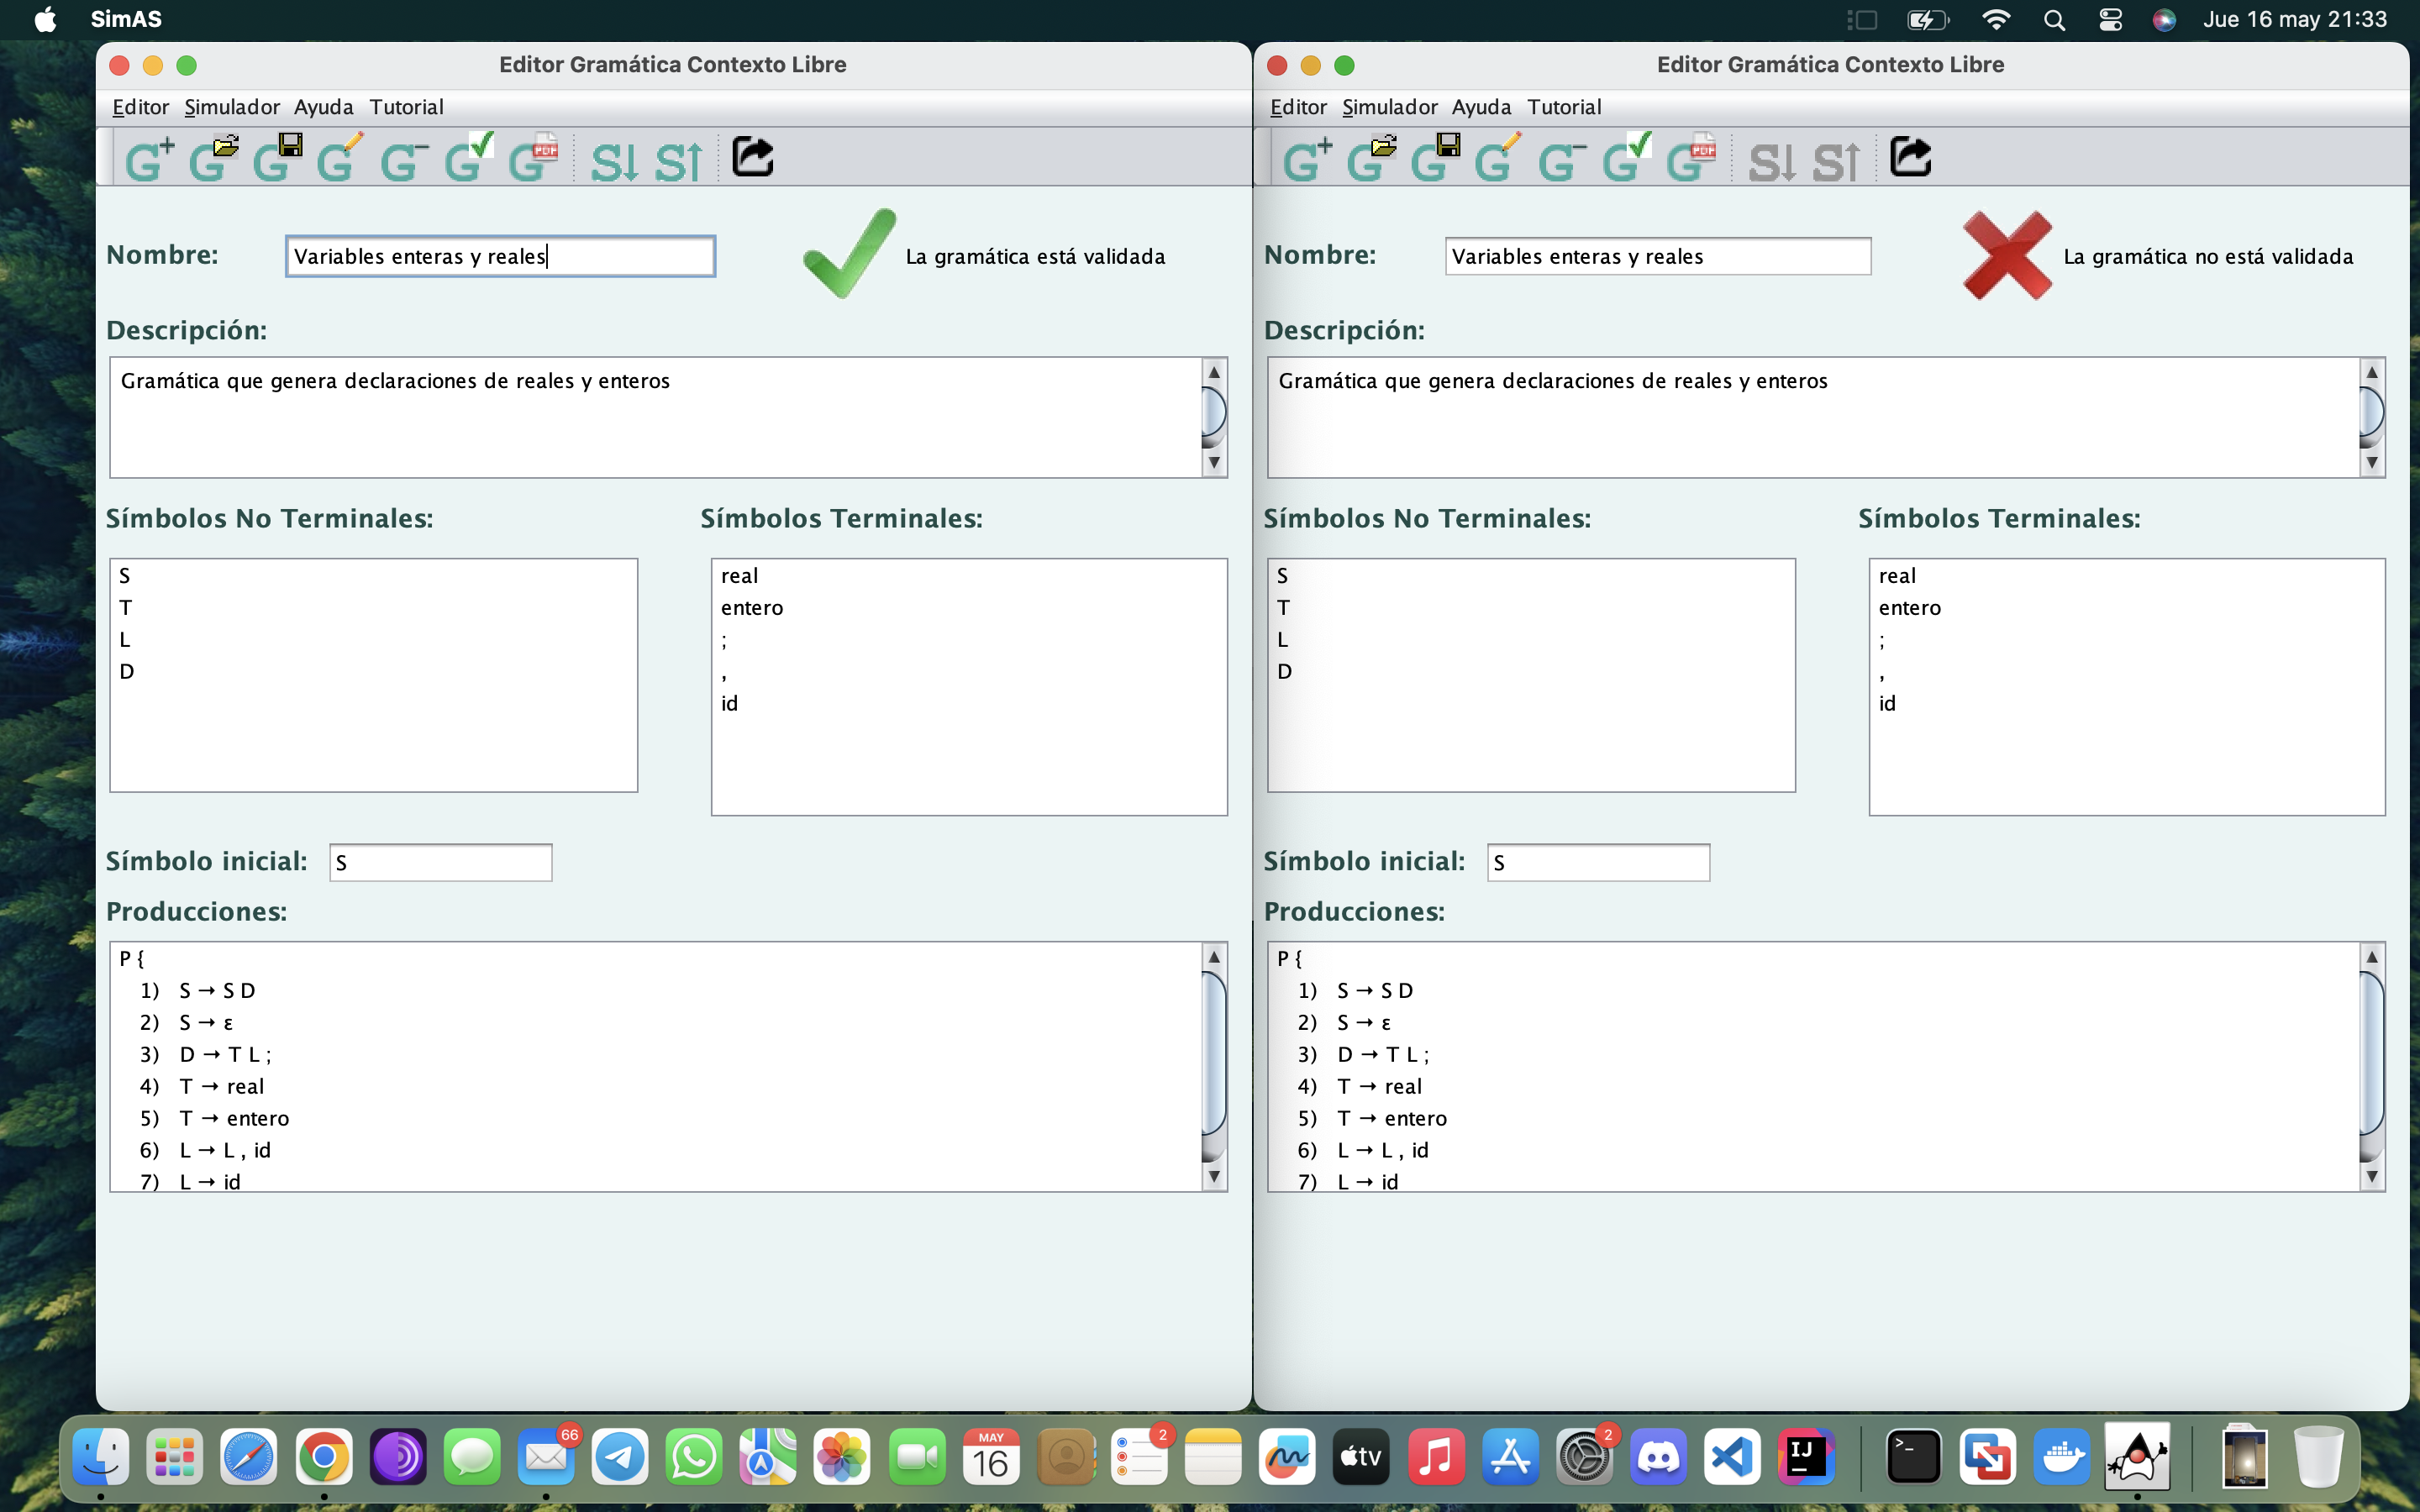
\includegraphics[scale=0.3]{figuras/Cap3/SimAS2/fallos/macos1.png} 
       \caption{Abrir gramática en MacOS.}\label{fig:SimAS-2.0-macos1}
 	\end{center}
\end{figure}

La aplicación no permite numerar las reglas de la gramática, lo que dificulta la identificación y referencia de las reglas durante el proceso de desarrollo. Asimismo, la imposibilidad de cambiar el orden de las reglas gramaticales puede causar problemas al corregir errores o reorganizar la estructura de la gramática.

En ciertas situaciones, el programa no incluye automáticamente la función de terminar el análisis en la tabla de funciones de error, lo que puede afectar la experiencia del usuario al simular la gramática. Además, al agregar una nueva regla de error, no se asigna automáticamente el siguiente número disponible, lo que puede resultar en la duplicación de números de reglas y generar confusión en la identificación de errores.

El informe generado por la aplicación no se visualiza correctamente en macOS, ya que al intentar abrirlo aparece un error al cargar el documento PDF. Este problema afecta la capacidad del usuario para revisar y analizar los resultados de la simulación de manera efectiva.

Al intentar modificar las funciones de error en la tabla predictiva, el programa duplica los símbolos no terminales en las filas y cambia los estados de la tabla predictiva, como se puede ver enla imagen \ref{fig:SimAS-2.0-macos2}. Este comportamiento inesperado puede causar errores en la interpretación de la tabla y afectar la precisión del análisis sintáctico.

\begin{figure}[htp]
 	\begin{center}
      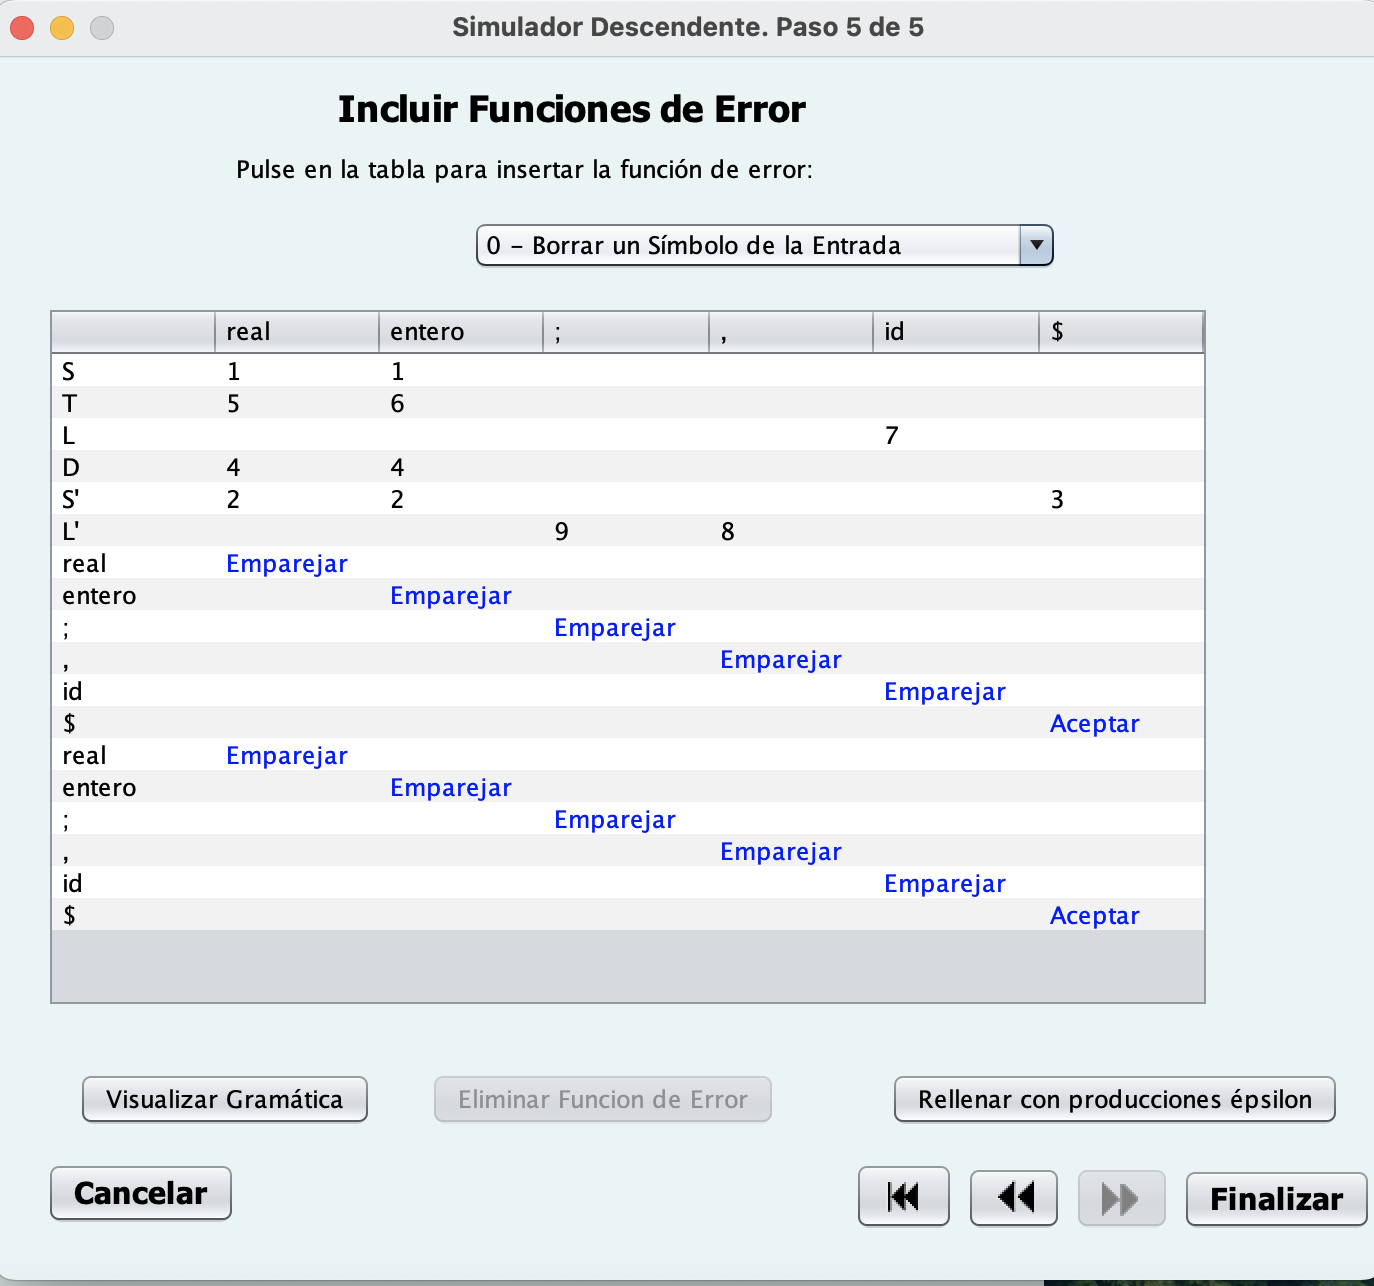
\includegraphics[scale=0.5]{figuras/Cap3/SimAS2/fallos/macos2.png} 
       \caption{Duplicación símbolos no terminales MacOS}\label{fig:SimAS-2.0-macos2}
 	\end{center}
\end{figure}

Durante la simulación descendente, la aplicación no permite incluir la cadena de entrada, lo que limita la capacidad del usuario para probar diferentes cadenas de entrada y verificar la precisión del análisis sintáctico. Además, al realizar la simulación descendente y agregar la declaración, la ventana emergente no se cierra automáticamente al aceptar la acción, lo que puede resultar en una experiencia de usuario inconsistente y confusa.


%Cambiar mayusculas por minusculas despues de :
\section{Justificación del trabajo} \label{sec:justificacion}

El desarrollo del presente Trabajo de Fin de Grado está justificado porque puede mejorar la versión anterior de la aplicación SimAS 2.0 \cite{juan}, que a su vez es una evolución de la primera versión desarrollada anteriormente \cite{vanesa}. Esta justificación se fundamenta en varios aspectos relevantes:

\begin{enumerate}
    \item \textbf{Corrección de problemas detectados}: la detección de algunos problemas y limitaciones en la versión anterior de SimAS 2.0 ha evidenciado la necesidad de realizar mejoras significativas. Estos problemas han obstaculizado el aprendizaje completo de los análisis sintácticos ascendentes y descendentes, lo que motiva la búsqueda de soluciones efectivas.
    
    \item \textbf{Mejora del aprendizaje interactivo}: se espera que la mejora y corrección de la aplicación conduzca a un funcionamiento más completo y correcto, lo que facilitará el aprendizaje profundo de los conceptos relacionados con los análisis sintácticos. Este enfoque interactivo no solo beneficia a los estudiantes, sino que también puede ser una herramienta valiosa para los profesores en la enseñanza de la asignatura de Procesadores de Lenguajes.
    
    \item \textbf{Impacto en el ámbito educativo y académico}: el desarrollo de una herramienta de aprendizaje interactiva como SimAS 3.0 tiene el potencial de tener un impacto significativo en el ámbito educativo y académico. Proporciona una oportunidad para mejorar la comprensión y el dominio de conceptos complejos en el campo de la informática, especialmente en lo relacionado con el procesamiento de lenguajes.
    
    \item \textbf{Continuidad y evolución del proyecto}: al seguir la evolución del proyecto desde la versión original hasta la actual, se establece una continuidad en la mejora y perfeccionamiento de la aplicación. Esta progresión refleja un compromiso constante con la excelencia y la adaptación a las necesidades cambiantes de los usuarios y del entorno educativo.
    
    \item \textbf{Facilitación del aprendizaje mediante una interfaz intuitiva}: la implementación de una interfaz más intuitiva y amigable con el usuario tiene como objetivo principal hacer que el proceso de aprendizaje sea más accesible y efectivo para los estudiantes. Esta mejora se alinea con las tendencias actuales en el diseño de herramientas educativas, que buscan maximizar la usabilidad y la experiencia del usuario.

    \item \textbf{Innovación y avance tecnológico}: la mejora y actualización de SimAS 3.0 representa un avance en la aplicación de nuevas tecnologías y metodologías en el campo de la educación informática. Este enfoque innovador busca aprovechar al máximo las capacidades de las herramientas digitales para mejorar la calidad y efectividad del aprendizaje.

    \item \textbf{Fomento del desarrollo profesional}: la participación en este proyecto brinda la oportunidad de adquirir y desarrollar habilidades técnicas y profesionales relevantes, como el diseño de software, la programación en Java y el trabajo en equipo. Estas habilidades son altamente valoradas en el mercado laboral y contribuyen al crecimiento profesional del estudiante.
    
    \item \textbf{Contribución a la comunidad académica}: al compartir los resultados y el código fuente de SimAS 3.0, se contribuye al conocimiento colectivo y se fomenta la colaboración entre instituciones educativas y profesionales del campo de la informática. Esta contribución puede dar lugar a nuevas investigaciones y desarrollos en el área de los procesadores de lenguajes y la educación informática en general.
    
    \item \textbf{Relevancia y aplicabilidad práctica}: la aplicación de SimAS 3.0 no solo se limita al ámbito académico, sino que también tiene aplicaciones prácticas en la industria y el desarrollo de software. La comprensión profunda de los análisis sintácticos que proporciona la herramienta es fundamental para el diseño y la implementación de compiladores y otros sistemas de procesamiento de lenguajes en la práctica profesional.

\end{enumerate}

En resumen, la realización de este trabajo se justifica por la necesidad de mejorar y perfeccionar una herramienta educativa clave en el ámbito de la informática, con el fin de proporcionar una experiencia de aprendizaje más efectiva y enriquecedora para los estudiantes.


\subsection{Comparativa entre versiones}
La Tabla \ref{tlb:tabla3_1} muestra, brevemente, una comparativa de las versiones 1.0 y lo que se pretendió alcanzar con la nueva versión 2.0 de SimAS, además de una comparativa con las características esperadas en la nueva versión, ``SimAS 3.0 descendente preditivo''. 

%Revisar tabla
\begin{center}
 \begin{table}[H]
 \caption{Comparación entre versiones de SimAS.}\label{tlb:tabla3_1}
 \resizebox{15cm}{!} 
 {
 \begin{tabular}[c]{| l | c | c | c |}
 \hline
   & \textbf{SimAS 1.0} & \textbf{SimAS 2.0} & \textbf{SimAS 3.0}  \\ 
   &   & & \textbf{descendente predictivo}  \\ \hline
  Edición de gramáticas de contexto libre & Sí & Sí & Sí  \\ \hline
  Análisis sintáctico descendente & Sí & Sí & Sí  \\ \hline
  Análisis sintáctico ascendente & Sí & Sí & No \\ \hline
  Generación de árboles sintácticos & No & Parcial & Sí  \\ \hline
  Generación de informes & No & Parcial & Sí \\ \hline
  Definición de funciones predefinidas & \multirow{2}*{No}  & \multirow{2}*{Parcial} & \multirow{2}*{Sí}   \\ 
   de tratamiento de errores &  &  &  \\ \hline 
   Compatibilidad multiplataforma & Parcial & Parcial & Sí \\ \hline
 \end{tabular}
 }
 \end{table}
\end{center}
\chapter{Restricciones} \label{cap:restricciones}

\section{Introducción}

Las restricciones técnicas y estratégicas son elementos fundamentales que limitan el diseño y la implementación del sistema. En este capítulo, se analizarán detalladamente los factores que restringen o condicionan el proyecto en diversas áreas. Se pueden identificar dos tipos principales de restricciones:

\begin{itemize}
    \item \textbf{Restricciones iniciales}: estas limitaciones son impuestas por la naturaleza misma del proyecto o por las condiciones ambientales en las que se desarrollará. Son estáticas y no pueden ser modificadas o eliminadas a lo largo del proceso de desarrollo. Por ejemplo, el tiempo del que se dispone para completar el proyecto podría considerarse una restricción inicial, ya que es un factor que no puede ser alterado una vez que se ha establecido un cronograma.
    
    \item \textbf{Restricciones estratégicas}: se refieren a variables de diseño que ofrecen varias alternativas. Durante el desarrollo del sistema, se elegirán aquellas opciones que se consideren más adecuadas en función de los objetivos y requisitos del proyecto. Por ejemplo, la elección entre diferentes tecnologías de base de datos podría ser una restricción estratégica.
\end{itemize}

\section{Factores iniciales} \label{sec:iniciales}

\subsection{Límites temporales}

Los límites temporales son un factor inicial crucial a considerar en el desarrollo del proyecto. Se establece como objetivo la presentación de la nueva versión de la aplicación en septiembre de 2024. Dado el tiempo disponible, se contempla priorizar el perfeccionamiento del análisis sintáctico descendente y la mejora general de la aplicación. 

\subsection{Entorno de software}

La nueva versión de la aplicación se basa en la infraestructura existente de SimAS 2.0 \cite{juan}, desarrollada previamente en Java \cite{java} y Java Swing \cite{javaswing} para la gestión de la interfaz gráfica. Se enfocará en corregir las funcionalidades defectuosas de la versión anterior y en agregar nuevas características para mejorar la experiencia del usuario y la eficiencia del programa.

Se continuará utilizando XML como lenguaje para la importación y exportación de gramáticas. Sin embargo, se realizarán ajustes en las definiciones de los elementos y características implementadas en la versión 2.0 para garantizar una mayor coherencia y modularidad en el manejo de las gramáticas.


% \subsection{Regulaciones y estándares de evaluación}
% En el ámbito académico, los Trabajos de Fin de Grado están sujetos a regulaciones y estándares establecidos por las instituciones educativas y los consejos evaluadores. Estas regulaciones son fundamentales para garantizar la calidad y el rigor académico de los proyectos presentados.
% Las regulaciones y estándares incluyen criterios de evaluación, formato y estructura del trabajo, normas académicas y éticas, plazos y fechas límite, así como requisitos adicionales. Cumplir con estas normativas es esencial para el éxito del presente Trabajo de Fin de Grado.


\section{Factores estratégicos} \label{sec:estrategicos}

\subsection{Metodología}

En esta subsección se presentarán diversas metodologías de desarrollo de software, cada una con enfoques y características distintivas. La selección de la metodología adecuada para el desarrollo del presente proyecto es crucial para su éxito. A continuación, se describen algunas de las metodologías más comunes:

\begin{enumerate}
    \item \textbf{Ciclo de vida en cascada:} este enfoque sigue una secuencia lineal de fases, donde cada fase se completa antes de pasar a la siguiente \cite{pressman}. Aunque fue ampliamente utilizado en el pasado, actualmente está en desuso debido a su rigidez y dificultad para adaptarse a los cambios en los requisitos del proyecto.
    
    \item \textbf{Desarrollo iterativo y incremental:} esta metodología implica el desarrollo y la entrega de funcionalidades en ciclos cortos y repetitivos. Es una metodología ampliamente utilizada en la actualidad, ya que permite una mayor flexibilidad y adaptación a medida que avanza el proyecto \cite{scrum}.
    
    \item \textbf{Metodología RAD (\textit{Rapid Application Development}):} esta metodología se centra en la rápida construcción de prototipos funcionales del software, con un enfoque en la entrega temprana de funcionalidades y la participación activa del cliente. Aunque ha perdido popularidad en los últimos años, sigue siendo utilizada en algunos proyectos donde el tiempo de desarrollo es crítico y los requisitos del sistema pueden no estar completamente definidos desde el principio \cite{rad}.

    \item \textbf{Metodología basada en UML (\textit{Unified Modeling Language}):} esta metodología se basa en el lenguaje de modelado unificado (UML) para el desarrollo de software. Aunque no es una metodología en sí misma, UML sigue siendo ampliamente utilizado en la industria del software como un marco estructurado y formal para el modelado y diseño de sistemas de software \cite{uml}.
\end{enumerate}

Dado que el presente proyecto implica el desarrollo de una aplicación de software, la metodología basada en UML \cite{uml}  se considera la más adecuada, porque proporciona un marco estructurado y formal para el modelado y diseño de software, lo que facilita la comprensión y el análisis de los requisitos del sistema. Además, UML es ampliamente utilizado en la industria del software y cuenta con un amplio conjunto de herramientas y recursos disponibles para su aplicación práctica.



\subsection{Lenguaje de programación}\label{sec:bases-de-datos}

La versión anterior de la aplicación SimAS 2.0 \cite{juan} utilizaba Java \cite{java} para el desarrollo de sus funcionalidades, así como Java Swing \cite{javaswing} para la interfaz gráfica. Además, para la carga y guardado de gramáticas, se empleaba XML \cite{xml}. 

Para esta nueva versión, se seguirán utilizando los mismos lenguajes de programación que en las ediciones anteriores. Java continuará siendo el lenguaje principal para implementar las funcionalidades, mientras que Java Swing se utilizará nuevamente para la creación de la interfaz gráfica. Sin embargo, se introducirá una diferencia significativa en el desarrollo de la interfaz de usuario. 

\subsection{Entorno de desarrollo}

Para llevar a cabo el desarrollo del proyecto, se consideraron varios entornos de desarrollo, entre ellos NetBeans \cite{netbeans} y IntelliJ IDEA \cite{intellij}. Inicialmente se contempló el uso de NetBeans debido a su familiaridad y uso previo en asignaturas del grado. Sin embargo, tras evaluar las opciones disponibles, se tomó la decisión de utilizar IntelliJ IDEA como el entorno de desarrollo principal, complementado con Scene Builder \cite{scenebuilder} para el diseño de interfaces gráficas.

\textbf{IntelliJ IDEA} ofrece numerosas ventajas que lo hacen especialmente adecuado para este proyecto. Entre ellas se incluyen:

\begin{itemize}
    \item \textbf{Interfaz intuitiva y potente}: IntelliJ IDEA cuenta con una interfaz de usuario intuitiva y altamente personalizable que facilita el desarrollo de aplicaciones Java.
    
    \item \textbf{Soporte integral para JavaFX y Scene Builder}: IntelliJ IDEA ofrece un soporte completo para el desarrollo de aplicaciones JavaFX, incluida la integración directa con Scene Builder para la creación de interfaces gráficas.
    
    \item \textbf{Funcionalidades avanzadas de refactorización y depuración}: El IDE proporciona potentes herramientas de refactorización de código y depuración, lo que permite mejorar la calidad del código y detectar y corregir errores de manera eficiente.
    
    \item \textbf{Amplia variedad de complementos y extensiones}: IntelliJ IDEA cuenta con una amplia gama de complementos y extensiones que permiten personalizar y ampliar sus funcionalidades según las necesidades del proyecto.
    
    \item \textbf{Integración con sistemas de control de versiones}: este IDE ofrece una integración perfecta con sistemas de control de versiones como Git, lo que facilita la colaboración en equipo y el seguimiento de cambios en el código.
\end{itemize}

La combinación de IntelliJ IDEA y Scene Builder proporciona un entorno de desarrollo completo y eficiente para la creación de la aplicación SimAS 3.0, permitiendo una experiencia de desarrollo fluida y productiva.


\subsection{Interfaz gráfica de la aplicación}

La interfaz gráfica de la aplicación SimAS 3.0 desempeña un papel fundamental en la experiencia del usuario, ya que proporciona una forma intuitiva y eficiente de interactuar con todas las funcionalidades del sistema. La interfaz ha sido diseñada con el objetivo de ser fácil de usar y estéticamente atractiva, manteniendo al mismo tiempo un alto nivel de funcionalidad y usabilidad.

La principal herramienta utilizada para el diseño de la interfaz gráfica es Scene Builder, que permite crear y modificar las interfaces de usuario de manera visual, utilizando componentes gráficos predefinidos y arrastrándolos y soltándolos en la ventana de diseño. Esto facilita enormemente el proceso de diseño y permite una rápida iteración para ajustar y mejorar la apariencia y la disposición de los elementos de la interfaz.

La interfaz gráfica de SimAS 3.0 se compone de varias secciones principales:

\begin{itemize}
    \item \textbf{Barra de menú}: proporciona acceso a todas las funcionalidades de la aplicación, incluyendo la creación y edición de gramáticas, la ejecución de análisis sintáctico, la importación y exportación de archivos, y la configuración de preferencias.
    \item \textbf{Barra de herramientas}: ofrece acceso rápido a las funciones más utilizadas, como la creación de nuevas gramáticas, la apertura y guardado de archivos, y la ejecución de análisis sintáctico.
    
    \item \textbf{Editor de gramáticas}: permite al usuario crear, editar y guardar gramáticas de contexto libre de forma intuitiva, proporcionando un entorno de edición con resaltado de sintaxis y sugerencias de autocompletado para facilitar la escritura.
    
    \item \textbf{Área de visualización de resultados}: muestra los resultados del análisis sintáctico, incluyendo árboles de análisis sintáctico, conjuntos primero y siguiente, y otros datos relevantes para el usuario.
    
    \item \textbf{Panel de configuración}: Permite al usuario personalizar diferentes aspectos de la aplicación, como la apariencia de la interfaz, las preferencias de análisis sintáctico y las opciones de importación y exportación de archivos.
\end{itemize}

En resumen, la interfaz gráfica de SimAS 3.0 va a ser diseñada para proporcionar una experiencia de usuario intuitiva y eficiente, facilitando la realización de tareas relacionadas con el análisis sintáctico de gramáticas de contexto libre. Mediante el uso de herramientas como Scene Builder, se pretende crear una interfaz atractiva y funcional que satisfaga las necesidades y expectativas de los usuarios. Véase la sección \ref{sec:requisitos_interfaz} de Requisito de la Interfaz y el capítulo \ref{cap:diseño_interfaz} del Diseño de la Interfaz.

\subsection{Sistema Operativo}

El correcto funcionamiento de la aplicación SimAS 3.0 se asegura mediante su ejecución en una máquina virtual Java (JVM) \cite{java}, lo que garantiza su compatibilidad y portabilidad en una amplia variedad de sistemas operativos. Este enfoque permite que la aplicación sea ejecutable de manera consistente en plataformas como Windows, macOS y Linux, independientemente de las diferencias en el entorno de ejecución subyacente.

Específicamente, en el caso de macOS Sonoma versión 14.0 \cite{macos}, se han llevado a cabo pruebas exhaustivas para asegurar que la aplicación se ejecute sin problemas en este sistema operativo. La JVM actúa como una capa de abstracción que permite que el código Java se ejecute de manera uniforme en diferentes sistemas, lo que garantiza una experiencia de usuario consistente y confiable.

La utilización de una máquina virtual Java también facilita la gestión de recursos y la optimización del rendimiento de la aplicación en el entorno de macOS Sonoma versión 14.0. Se han implementado las mejores prácticas de desarrollo de software para aprovechar al máximo las características específicas de este sistema operativo y garantizar una ejecución eficiente de la aplicación.

En resumen, SimAS 3.0 se ejecutará en una máquina virtual Java para garantizar su compatibilidad y portabilidad en macOS Sonoma versión 14.0, así como en otros sistemas operativos, asegurando que los usuarios puedan acceder a todas sus funcionalidades sin importar la plataforma que utilicen.

\subsection{Representación de las gramáticas de contexto libre}

Para almacenar la información de las gramáticas de contexto libre creadas por el usuario, se seguirá usando el formato XML \cite{xml} como en las versiones anteriores. Este formato proporciona una estructura definida que asegura la seguridad y la compatibilidad de los datos entre diferentes sistemas. Esta nueva versión SimAS 3.0 explorará la posibilidad de mejorar la organización de los archivos XML de las gramáticas para facilitar su comprensión y manipulación.

\subsection{Generación de informes de gramáticas y de simulación}

Cada gramática creada con la aplicación podrá ir acompañada de un informe detallado que contenga toda la información pertinente. Del mismo modo, tras realizar una simulación, se ofrecerá la opción de generar informes con los resultados obtenidos, incluyendo todos los diagramas relevantes.

Se identificó un problema en la versión SimAS 2.0 relacionado con la generación inconsistente de informes en algunos sistemas operativos. Se investigará a fondo esta cuestión y se implementarán las correcciones necesarias para garantizar que los informes se generen correctamente en todas las plataformas compatibles. 

Además, se planea continuar generando los informes en formato \textbf{PDF}, debido a su amplia aceptación y su resistencia a ser alterado, lo que facilitaría su distribución y aumentaría su accesibilidad. También se estudiará la viabilidad de generar los informes en otros formatos para adaptarse a las necesidades específicas de los usuarios.

\subsection{Implementación de la ayuda}

La implementación de la ayuda del programa es un aspecto crucial para proporcionar una experiencia de usuario satisfactoria. En este sentido, se están considerando dos enfoques distintos para llevar a cabo esta tarea:

Por un lado, se contempla la posibilidad de mantener la misma metodología utilizada en la versión anterior del programa. Esta metodología consiste en emplear una página web para proporcionar la ayuda necesaria. Esta opción tiene la ventaja de ser familiar para los usuarios que hayan utilizado versiones anteriores de la aplicación. Además, la generación de la ayuda en formato HTML \cite{html} facilita su integración con la interfaz de usuario desarrollada en Java \cite{java}, lo que permite una navegación fluida y una experiencia coherente para el usuario.

Por otro lado, se está evaluando la opción de implementar la ayuda como parte integral de la interfaz de usuario del programa. Esta alternativa implicaría integrar una sección de ayuda directamente dentro de la ventana principal de la aplicación. Esta sección podría presentarse mediante pestañas, paneles desplegables u otros elementos de navegación, proporcionando así un acceso rápido y sencillo a la información relevante. Este enfoque aprovecharía las capacidades de la interfaz gráfica de usuario para ofrecer una experiencia más intuitiva y cohesiva para el usuario.

La elección entre estas dos opciones dependerá de diversos factores, como la complejidad de la ayuda requerida, las preferencias del usuario y las limitaciones de desarrollo. Ambos enfoques tienen sus ventajas y desventajas, por lo que se llevará a cabo un análisis detallado para determinar cuál de ellos se adapta mejor a las necesidades y objetivos del proyecto.

\subsection{Implementación del tutorial}

El tutorial se mantendrá en formato PDF y se incluirá junto con la aplicación para proporcionar a los usuarios una guía detallada sobre el funcionamiento del análisis sintáctico. 

Este tutorial estará diseñado para abordar de manera clara y concisa los conceptos teóricos fundamentales del análisis sintáctico, así como para ofrecer ejercicios prácticos que permitan a los usuarios poner en práctica lo aprendido y afianzar su comprensión. De esta manera, se pretende facilitar el aprendizaje y la familiarización de los usuarios con el uso de la aplicación, brindándoles una herramienta efectiva para mejorar sus habilidades en el análisis sintáctico de gramáticas.

\subsection{Representación de los árboles sintácticos}

Como novedad introducida en SimAS 2.0 \cite{juan}, se implementó la generación de árboles sintácticos de manera iterativa y paralela al análisis sintáctico. En la versión actual, SimAS 3.0, se busca mejorar esta funcionalidad basándose en la experiencia previa con la herramienta Graphviz \cite{graphviz}. Se ha decidido continuar utilizando Graphviz debido a su facilidad de uso y su capacidad para generar árboles gráficos de manera efectiva. Esta decisión se toma con el objetivo de partir de una base sólida y mejorar los puntos en los que la versión anterior presentaba deficiencias en la representación de árboles sintácticos.


\chapter{Recursos}

En este capítulo se expondrán los recursos usados durante la realización de este proyecto. Los recursos se definen como aquellos medios de los que se dispone para abordar el proceso de desarrollo del proyecto.

Existen tres grupos de recursos:

 \begin{itemize}
     \item Recursos humanos.
     \item Recursos de hardware.
     \item Recursos de software.
 \end{itemize}


 \section{Recursos humanos}
 \begin{itemize}
     \item \textbf{Autor}
     \item[] Antonio Llamas García, estudiante del Grado en Ingeniería Informática, especialidad en Computación.
    
     \item \textbf{Director}
     \item[] Dr. Nicolás Luis Fernández García. Profesor Titular de Universidad del área de Ciencia de la Computación e Inteligencia Artificial, perteneciente al Departamento de Informática y Análisis Numérico de la Universidad de Córdoba.
 \end{itemize}

\section{Recursos de hardware}
 Durante el desarrollo del proyecto se empleará el equipo informático a disposición del autor, cuya descripción corresponde con:
  \begin{itemize}
      \item Ordenador Portátil Características:
      \begin{itemize}
         \item Procesador Intel(R) Core(TM) 2,4 GHz i5 de 4 núcleos
         \item 16 Gbytes de memoria RAM.
         \item Intel Iris Plus Graphics 655 1536 MB.
         \item Almacenamiento: 240 Gb SSD.
      \end{itemize}
  \end{itemize}

\section{Recursos de software}
Se empleará Scene Builder \cite{scenebuilder} junto con JavaFX \cite{javafx} para, el lugar de diseñar la interfaz manualmente programando, realizar este cometido de una forma mucho más intuitiva. Scene Builder es una herramienta que permite diseñar interfaces gráficas de manera visual para aplicaciones JavaFX. Esta elección se debe al hecho de que Scene Builder trabaja con JavaFX, lo que facilitará una creación más intuitiva y eficiente de la interfaz de usuario, mejorando así el proceso de desarrollo.

Además, se modularizarán las características de los elementos de los ficheros XML de gramáticas, permitiendo una separación más clara y una gestión más eficiente de los datos. Finalmente, se mejorará el uso de Graphviz \cite{graphviz}, una biblioteca utilizada en la versión anterior, para permitir la generación de los árboles sintácticos de forma iterativa, mejorando así la visualización y comprensión de los resultados del análisis sintáctico.

 \subsection{Sistema Operativos}
 \begin{itemize}
      \item MacOs Sonoma, versión 14.0
  \end{itemize}

 
  \subsection{Entorno de desarrollo y lenguaje de programación}
  \begin{itemize}
      \item IntelliJ IDEA\cite{intellij}: entorno de desarrollo utilizado para la codificación y pruebas de la aplicación.
      \item Java \cite{java}: lenguaje de programación multiplataforma.
      \item Java Swing \cite{javaswing}: biblioteca de Java para el desarrollo de aplicaciones gráficas.
  \end{itemize}

 \subsection{Herramientas de documentación}
  \begin{itemize}
      \item \LaTeX \ \cite{latex}: software de formateo de documentación científica y técnica.
      \item OverLeaf \cite{overleaf}: \textit{front-end} web para \LaTeX.
  \end{itemize}

  \subsection{Herramientas para la edición de diagramas}
  \begin{itemize}
      \item Draw.io (Diagrams.net) \cite{drawio}: editor gráfico para el diseño de los diagramas.
  \end{itemize}


\part{Análisis}
\chapter{Especificación de requisitos}\label{cap:especificacion_requisitos}

\section{Introducción}

Este capítulo se dedica a la especificación detallada de los requisitos del sistema, abarcando tanto los requisitos \textit{funcionales} como los \textit{no funcionales}, así como los requisitos de \textit{información} y de \textit{interfaz}. Antes de entrar en los detalles específicos de estos requisitos, se proporciona una descripción funcional del simulador, resaltando los módulos identificados previamente. Posteriormente, se identificarán los actores que interactuarán con la aplicación.

\section{Actores} \label{sec:actores-req}

El software diseñado en este proyecto está destinado a un entorno educativo, dirigido principalmente a \textit{profesores} y \textit{estudiantes}. A pesar de esta diferenciación en los roles, la aplicación no distinguirá funcionalmente entre estos usuarios, ya que ambos tendrán acceso a las mismas funcionalidades. Por lo tanto, cualquier referencia a los \textit{actores} de la aplicación se aplicará de manera uniforme a todos los usuarios finales, independientemente de su rol específico.


\section{Descripción modular del sistema}

El sistema se compone de varios módulos integrados, cada uno con un propósito específico. A continuación, se describen en detalle los módulos principales que conforman la aplicación:

\begin{itemize}
\item Editor de gramáticas.
\item Simulador gráfico descendente.
\item Tutorial.
\item Sistema de ayuda.
\end{itemize}

 La Figura \ref{fig:diagrama-descomposicion} muestra la descomposición modular del sistema.
 
\begin{figure}[!ht]
   \begin{center} 
     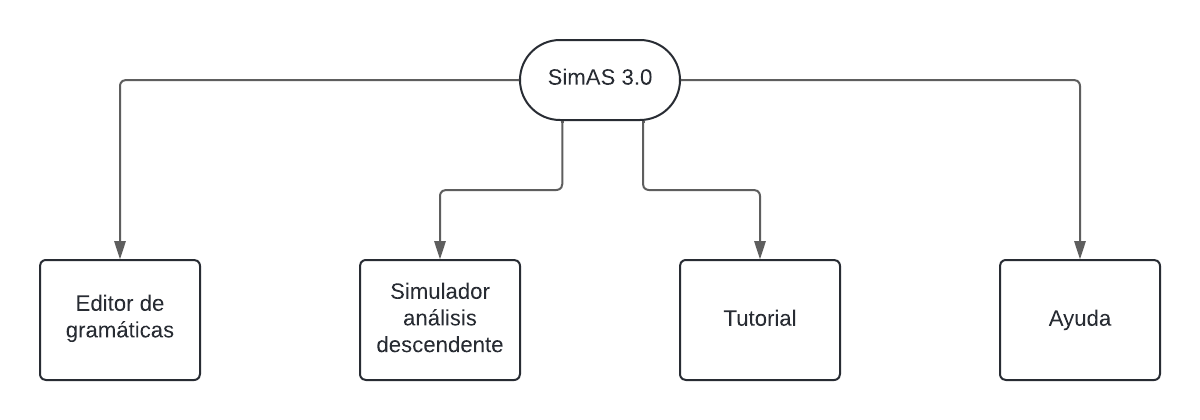
\includegraphics[width=1\textwidth]{figuras/Cap6/diagrama-descomposicion.png}
     \caption{Descomposición modular del sistema}\label{fig:diagrama-descomposicion}
   \end{center}
 \end{figure}


\subsection{Módulo del Editor de Gramáticas}

El editor de gramáticas es una herramienta fundamental dentro del sistema, permitiendo a los usuarios crear y modificar gramáticas de contexto libre. Las funcionalidades específicas de este módulo incluyen:

\begin{enumerate}
    \item \textbf{Creación de gramáticas}: los usuarios pueden definir nuevas gramáticas, especificando sus componentes esenciales, como símbolos terminales, no terminales, el símbolo inicial y las reglas gramaticales.
    \item \textbf{Gestión de vocabulario}: permite a los usuarios añadir y eliminar símbolos del vocabulario de una gramática, gestionando tanto los símbolos terminales como los no terminales, que son necesarios para formar las reglas.
    \item \textbf{Gestión de reglas gramaticales o producciones}: facilita la introducción, modificación y eliminación de las reglas gramaticales de una gramática, asegurando que no haya duplicados.
    \item \textbf{Validación de gramáticas}: este proceso asegura que la gramática es válida, verificando que todos los símbolos sean accesibles y generadores:
    \begin{itemize}
        \item \textbf{Accesibilidad}: un símbolo se considera accesible si se puede alcanzar desde el símbolo inicial mediante una serie de derivaciones.
        \item \textbf{Generatividad}: un símbolo es generativo si puede derivar en una cadena de símbolos terminales o la cadena vacía.
    \end{itemize}
    
    En caso de errores, se informará al usuario y se proporcionarán sugerencias para la corrección.
    \item \textbf{Almacenamiento de gramáticas}: los usuarios pueden guardar sus gramáticas en archivos para uso futuro, independientemente de si la gramática ha sido completamente validada.
    \item \textbf{Carga de gramáticas}: permite cargar gramáticas desde archivos existentes, validando que no estén corruptos y notificando al usuario  cualquier error durante el proceso.
    \item \textbf{Consulta de gramáticas}: muestra la estructura completa de la gramática actual, incluyendo todos sus componentes, y permite generar un informe detallado.
\end{enumerate}

\subsection{Módulo del Simulador Gráfico Descendente Predictivo}

Este módulo constituye el núcleo de la aplicación, proporcionando la capacidad de simular el análisis sintáctico descendente predictivo de manera visual e interactiva. A continuación se detalla su funcionamiento.

\subsubsection{Creación y carga de gramáticas}

El primer paso en el proceso de simulación es la creación o carga de una gramática. Los usuarios pueden utilizar el módulo de edición de gramáticas para definir una nueva gramática o cargar una existente desde un archivo. Es fundamental que la gramática haya sido validada previamente para asegurar su correcta estructura y funcionalidad antes de ser utilizada en la simulación.

\subsubsection{Generación de conjuntos \textit{Primero} y \textit{Siguiente}}

Una vez que la gramática está lista, se procede a la generación de los conjuntos Primero y Siguiente. Estos conjuntos son esenciales para la construcción de la tabla predictiva, ya que determinan las posibles reglas gramaticales o producciones que pueden aplicarse durante el análisis de una cadena de entrada.

\subsubsection{Construcción de la tabla predictiva}

Después de obtener los conjuntos Primero y Siguiente, se debe construir la tabla predictiva del análisis sintáctico descendente. Esta tabla es una guía que indica qué regla gramatical debe aplicarse para cada combinación de símbolo de entrada y símbolo no terminal. La tabla predictiva es fundamental para la correcta derivación de la cadena de entrada y facilita la detección y manejo de errores durante el análisis.

\subsubsection{Implementación de funciones de recuperación de errores}

Aunque esta parte es opcional, la implementación de funciones de recuperación de errores es altamente recomendable. Estas funciones se utilizan para manejar las celdas vacías en la tabla predictiva, proporcionando mecanismos para continuar el análisis sintáctico en caso de encontrar un error. Entre las funciones de recuperación de errores se incluyen:

\begin{itemize}
  \item Eliminar el símbolo actual de la entrada.
  \item Insertar un nuevo símbolo terminal en la entrada, con funciones específicas para cada símbolo terminal.
  \item Terminar el análisis si hay un final inesperado de la entrada.
\end{itemize}

\subsubsection{Simulación del análisis sintáctico descendente  predictivo}

Con la tabla predictiva completada, el usuario puede introducir una cadena de entrada para simular el análisis sintáctico descendente predictivo. Durante esta fase, el simulador utilizará la tabla predictiva para derivar la cadena de entrada, gestionando los errores según las funciones de recuperación definidas. El sistema informará al usuario sobre el estado de la cadena de entrada, indicando si es reconocida o si se han producido errores. La aplicación permitirá mostrar la derivación de la cadena de entrada generada por el análisis sintáctico descendente predictivo.

\subsubsection{Generación del árbol sintáctico descendente}

Una característica avanzada del simulador es la capacidad de generar el árbol sintáctico descendente. Esta opción permite a los usuarios visualizar la estructura jerárquica de la derivación de la cadena de entrada en tiempo real, mejorando su comprensión del proceso de análisis sintáctico. El árbol sintáctico se construye de forma paralela a la simulación, proporcionando una representación gráfica de cada paso del análisis.

\subsubsection{Creación de informes}

Finalmente, tras la simulación, se generará un informe detallado que documenta todo el proceso. Este informe, disponible en formatos PDF o HTML, incluirá:

\begin{itemize}
  \item Información detallada sobre la gramática utilizada.
  \item Los conjuntos Primero y Siguiente generados.
  \item La tabla predictiva construida.
  \item Las funciones de recuperación de errores definidas.
  \item La cadena de entrada y su estado (reconocida o no).
  \item Los errores detectados durante el análisis y cómo fueron manejados.
  \item La derivación de la cadena de entrada generada por el análisis sintáctico descendente predictivo.
  \item El árbol sintáctico asociado a la derivación de la cadena de entrada generada por el análisis sintáctico descendente predictivo.
\end{itemize}

Este informe puede ser almacenado en disco por el usuario, proporcionando una referencia completa y detallada del análisis sintáctico descendente realizado.


\subsection{Módulo del Tutorial}

Este módulo tiene un enfoque educativo, diseñado para proporcionar todos los objetivos pedagógicos del proyecto. Se ubicará de manera accesible desde cualquier otro módulo del programa, permitiendo al usuario consultarlo en cualquier momento, incluso mientras interactúa con otras partes de la aplicación.

\subsubsection{Estructura del tutorial}

El tutorial se organizará en las siguientes secciones:

\begin{enumerate}
    \item \textbf{Introducción y fundamentos teóricos:} esta sección cubre los conceptos teóricos fundamentales del análisis sintáctico, con un enfoque en las gramáticas de contexto libre. Proporcionará una base sólida para entender los principios detrás del análisis sintáctico descendente.

    \item \textbf{Lecciones de análisis sintáctico descendente:} aquí se explicarán los métodos de análisis sintáctico descendente predictivo. Las lecciones estarán estructuradas de manera que el usuario pueda seguir cada paso del proceso de análisis de manera clara y comprensible.

    \item \textbf{Ejemplos y ejercicios prácticos:} esta parte del tutorial incluirá una serie de ejercicios prácticos y ejemplos resueltos. Los usuarios podrán realizar estos ejercicios y verificar sus respuestas utilizando el simulador. Esta sección está diseñada para reforzar el aprendizaje a través de la práctica y la aplicación de conceptos teóricos.
\end{enumerate}

\subsection{Módulo de Ayuda}

El módulo de \textit{Ayuda} proporciona una guía completa sobre el uso de la aplicación. Está diseñado para ser una referencia detallada que abarca todos los aspectos del funcionamiento del programa.

\subsubsection{Contenidos de la ayuda}

\begin{enumerate}
    \item \textbf{Introducción a la aplicación:}
    esta sección presentará una visión general de la aplicación, describiendo sus objetivos y las principales funcionalidades que ofrece. Proporcionará una primera impresión de lo que los usuarios pueden esperar del programa.

    \item \textbf{Requisitos de instalación y procedimiento:}
    aquí se detallarán los requisitos del sistema necesarios para ejecutar la aplicación, así como las instrucciones paso a paso para su instalación y desinstalación. Se incluirán también soluciones a posibles problemas que puedan surgir durante estos procesos.

    \item \textbf{Guía de la interfaz de usuario:}
    esta sección ofrecerá una explicación detallada de los diferentes componentes de la interfaz del simulador. Se proporcionarán descripciones de cada elemento de la interfaz y su funcionalidad, ayudando a los usuarios a navegar y utilizar el programa de manera eficiente.

    \item \textbf{Descripción de los módulos del programa:}
    En esta parte, se explicará en profundidad el funcionamiento de cada uno de los módulos de la aplicación. Se incluirán instrucciones específicas sobre cómo utilizar cada módulo, junto con ejemplos prácticos y consejos para maximizar su uso.
\end{enumerate}


 \section{Requisitos funcionales}

En esta sección se recogen los requisitos funcionales de la aplicación, los cuales se denotarán como \textbf{RF-$<$acrónimo del módulo$>$-$<$número de requisito$>$}. Los requisitos funcionales se encuentran agrupados según los módulos funcionales del Sistema, que son las siguientes:

\begin{itemize}
 \item \textbf{Editor de gramáticas}: requisitos funcionales del \textit{editor de gramáticas}.
 \item \textbf{Simulador}: requisitos funcionales del \textit{simulador}.
 \item \textbf{Tutorial}: requisitos funcionales del \textit{tutorial}.
 \item \textbf{Ayuda}: requisitos funcionales  del \textit{ayuda}.
\end{itemize}


\subsection{Requisitos funcionales del Editor de gramáticas}\label{sec:requisitos-funcionales-editor}

Esta sección detalla todos los requisitos funcionales del \textit{Editor de gramáticas}, listados a continuación:

\begin{itemize}
    \item \textbf{RF-E-1}. El editor de gramáticas permitirá al usuario crea una nueva gramática de contexto libre. 
    \item \textbf{RF-E-2}. El editor permitirá la creación y modificación del conjunto de símbolos de la gramática (símbolos terminales y no terminales):
    \begin{itemize}
      \item \textbf{RF-E-2.1}. También admitirá el uso de caracteres especiales, tales como $\epsilon$ y $\rightarrow$, entre otros.
    \item \textbf{RF-E-2.2}. Será posible definir símbolos personalizados para la construcción de reglas, como, por ejemplo, $<$asignación$>$.
    \item  \textbf{RF-E-2.3}. Se gestionarán y notificarán todos los errores relacionados con la creación y edición de símbolos de manera clara y concisa para el usuario.
    \item \textbf{RF-E-2.4}. Las reglas de la gramática se ordenarán en función del símbolo no terminal de su parte izquierda.
    \end{itemize}
    
\item \textbf{RF-E-3}. El editor permitirá crear reglas gramaticales utilizando los símbolos definidos por el usuario. Se verificará que el \textit{antecedente} de cada regla es un \textit{único símbolo no terminal}.

\item \textbf{RF-E-4}. La inserción de reglas gramaticales estará controlada y se notificará al usuario cualquier error ocurrido. Si una regla es introducida más de una vez, el sistema lo advertirá y solamente permitirá una instancia de la misma.

\item \textbf{RF-E-5}. El editor permitirá la edición completa de las reglas gramaticales, pudiéndose modificar tanto el antecedente como el consecuente de cada regla. También será posible eliminar reglas de la gramática.

\item \textbf{RF-E-6}. Por defecto, el símbolo inicial de la gramática será el antecedente de la primera regla gramatical introducida. No obstante, el editor permitirá que el usuario lo modifique posteriormente si lo desea. La gramática debe tener un único símbolo inicial.

\item \textbf{RF-E-7}. Cada gramática tendrá un nombre y una descripción asignados por el usuario, los cuales podrán ser modificados en cualquier momento.

\item \textbf{RF-E-8}. La gramática se visualizará en el editor a medida que se construye. Se actualizará con cada nueva regla introducida y podrá ser visualizada en cualquier momento.

\item \textbf{RF-E-9}. El editor permitirá generar un informe detallado de la gramática actual. Este informe incluirá todos los elementos visualizados y componentes de la gramática, y podrá ser guardado en el disco según la preferencia del usuario.

\item \textbf{RF-E-10}. El editor permitirá cerrar la gramática en curso, notificando al usuario de la acción. Se ofrecerá la opción de guardar la gramática antes de cerrarla para evitar la pérdida de datos.

\item \textbf{RF-E-11}. La gramática actual podrá ser guardada en el disco para su uso posterior. Se solicitará al usuario un nombre para el archivo y la ubicación de almacenamiento, además de un nombre para la gramática si no se ha proporcionado anteriormente.

\item \textbf{RF-E-12}. El editor permitirá abrir una gramática previamente guardada desde un fichero y cargarla en el editor. Se controlarán todos los errores que puedan surgir durante esta operación y se notificarán al usuario si la gramática no puede ser cargada.

\item \textbf{RF-E-13}. La validación de la gramática comprobará que es adecuada para la simulación. Durante esta validación se revisarán los siguientes aspectos:
\begin{itemize}
    \item  \textbf{RF-E-13.1}. La gramática debe tener un único símbolo inicial (según lo especificado en \textbf{RF-E-6}).
    \item  \textbf{RF-E-13.2}. Todos los símbolos deben ser útiles, es decir, accesibles y generadores.
\end{itemize}

\item \textbf{RF-E-14}. Cualquier error identificado durante la validación será comunicado al usuario. No se permitirá continuar con la simulación si existen errores en la gramática. Si la validación es exitosa, se informará al usuario mediante un mensaje.

\item \textbf{RF-E-15}. El editor permitirá transferir gramáticas al simulador para llevar a cabo la simulación del análisis sintáctico descendente predictivo. Solo se podrán transferir aquellas gramáticas que hayan sido validadas con éxito. Esta acción inicializará el simulador y cargará la gramática para su simulación.

\end{itemize}

\subsection{Requisitos funcionales del Simulador}

\begin{itemize}
    \item \textbf{RF-S-1}. El simulador permitirá aplicar el método de análisis descendente predictivo.
  \begin{itemize}
      \item \textbf{RF-S-1.1}. Se deberá verificar que la gramática no presenta recursividad por la izquierda y está adecuadamente factorizada por la izquierda. En caso contrario, se aplicarán los algoritmos correspondientes. El usuario podrá consultar tanto la gramática original como la transformada.
  \end{itemize}

    \item \textbf{RF-S-2}. El simulador generará los conjuntos Primero y Siguiente, esenciales para el análisis sintáctico descendente predictivo.

    \item \textbf{RF-S-3}. El simulador construirá la \textit{tabla predictiva} y todos los elementos auxiliares necesarios para el método elegido.

    \item \textbf{RF-S-4}. En la tabla predictiva, el simulador permitirá el uso de funciones de manejo de errores para aplicar el método de nivel de frase de recuperación de errores. 

    \item \textbf{RF-S-5}. El simulador notificará cualquier error que ocurra durante la creación de las tablas.

    \item \textbf{RF-S-6}. Durante la simulación, las funciones de error serán invocadas en caso de que se produzca un error.

    \item \textbf{RF-S-7}. La simulación podrá iniciarse una vez que se haya generado la tabla predictiva, independientemente de que esté completada con funciones de error o no.

    \item \textbf{RF-S-8}. El simulador solicitará al usuario una cadena de entrada para verificar si es reconocida por el método de simulación. Esta cadena podrá ser vacía ($\epsilon$). Se controlarán todos los posibles errores de entrada-salida o de simulación.

    \item \textbf{RF-S-9}. Una vez creada la tabla predictiva e introducida la cadena de entrada, la simulación podrá comenzar de forma \textit{continua} o \textit{paso a paso}.

    \item \textbf{RF-S-10}. En la simulación continua, se mostrará el resultado final de la simulación en una tabla que incluirá todos los errores producidos, en su caso. La tabla se generará y se mostrará completa al usuario.

    \item \textbf{RF-S-11}. En la simulación paso a paso, se  mostrarán los resultados de la simulación progresivamente, construyendo la tabla de resultados de forma \textit{incremental} a medida que el usuario avance en la simulación.

    \item \textbf{RF-S-12}. Durante la simulación, ya sea automática o paso a paso, el simulador mostrará la construcción del árbol correspondiente al análisis sintáctico descendente.

    \item \textbf{RF-S-13}. El simulador informará al usuario de cualquier error que ocurra durante la simulación. Si existen funciones de manejo de errores asociadas, se utilizarán e informarán al usuario sobre el motivo de su uso.

    \item \textbf{RF-S-14}. Al finalizar, el simulador podrá generar un informe de la simulación en formato PDF o HTML. Este informe incluirá la gramática, su tabla de análisis, las funciones de error, la derivación generada y el árbol sintáctico construido.
    
    \item \textbf{RF-S-15}. Al finalizar, el simulador podrá mostrar la derivación generada por el análisis sintáctico predictivo.

    \item \textbf{RF-S-16}. Al finalizar, el simulador podrá el árbol sintáctico asociado a la derivación generada por el análisis sintáctico predictivo.

    \item \textbf{RF-S-17}. El simulador permitirá guardar el informe de simulación en el disco duro, indicando la gramática, la tabla predictiva,  las funciones de error, la tabla de simulación del análisis sintáctico, la derivación generado y el árbol sintáctico asociado.

    \item \textbf{RF-S-18}. Las simulaciones podrán ser abortadas, permitiendo al usuario cambiar la gramática o el conjunto de funciones de error. Se informará al usuario si desea conservar el trabajo realizado hasta ese momento y guardar los informes de simulación producidos (si los hay).
\end{itemize}



\subsection{Requisitos funcionales del Tutorial}

\begin{itemize}
    \item \textbf{RF-T-1}. El usuario podrá acceder al tutorial desde cualquier sección de la aplicación.
    \item \textbf{RF-T-2}. El tutorial estará dividido en lecciones que abarcarán todo el procedimiento de operación con los mecanismos del análisis sintáctico descendente predictivo.
\end{itemize}

\subsection{Requisitos funcionales de la Ayuda}

\begin{itemize}
    \item \textbf{RF-A-1}. La sección de ayuda será accesible desde cualquier parte de la aplicación.
    \item \textbf{RF-A-2}. La ayuda estará organizada en capítulos que cubrirán todos los módulos de la aplicación, proporcionando explicaciones detalladas de todos los procedimientos y utilizando ejemplos para ilustrar su uso.
\end{itemize}


\section{Requisitos no funcionales}
 En esta sección se detallan los requisitos no funcionales del Sistema, identificados como \textbf{RNF-$<$número de requisito$>$}.

\begin{itemize}
    \item \textbf{RNF-1}. La interfaz del sistema debe ser intuitiva y fácil de usar, centrada en facilitar la comprensión didáctica del análisis sintáctico. Se utilizarán menús fáciles de navegar, botones de acción y gráficos pertinentes a los métodos de análisis sintáctico. Además, deberá manejar errores de manera amigable, proporcionando mensajes claros y soluciones.
    \item \textbf{RNF-2}. La aplicación debe manejar adecuadamente todos los errores que ocurran durante su ejecución (errores de entrada-salida, de ejecución, de simulación, etc.).
    \item \textbf{RNF-3}. El sistema debe proporcionar respuestas a las solicitudes del usuario dentro de un tiempo razonable.
    \item \textbf{RNF-4}. La importación y exportación de gramáticas se hará utilizando el formato XML. Se buscará la máxima modularidad, diferenciando entre el antecedente y el consecuente junto con sus respectivos valores.
    \item \textbf{RNF-5}. Seguridad del sistema. El sistema debe estar protegido y asegurar una descarga segura tanto de informes como de gramáticas.
    \item \textbf{RNF-6}. Escalabilidad del sistema. El sistema debe ser capaz de adaptarse a aumentos o reducciones en sus módulos, integrando nuevos componentes o eliminando los innecesarios sin afectar a la funcionalidad general.
    \item \textbf{RNF-7}. Fiabilidad del sistema. El sistema debe ser confiable y cumplir con los requisitos especificados por el usuario.
    \item \textbf{RNF-8}. Compatibilidad del sistema. El sistema debe ser compatible con los sistemas operativos MacOS, Windows y Linux.
\end{itemize}


\section{Requisitos de la información}

En esta sección se especifican los requisitos de la información, identificados como \textbf{RI-$<$acrónimo del módulo$>$-$<$número de requisito$>$}. Estos requisitos se agrupan en función de los conceptos identificados durante la especificación de los requisitos del usuario.

Los requisitos de la información se organizan en los siguientes bloques de información:

\begin{itemize}
 \item \textbf{Gramática de contexto libre}: requisitos de información para la \textit{gramática de contexto libre}, que será un sub-módulo auxiliar del módulo \textit{editor de gramáticas}.
 
 \item \textbf{Editor de gramáticas}: requisitos de información para el módulo \textit{editor de gramáticas}.
 
 \item \textbf{Simulador}: requisitos de información para el módulo \textit{simulador} del análisis sintáctico descendente predictivo.
 
 \item \textbf{Ayuda de la aplicación}: requisitos de información para el módulo \textit{ayuda de la aplicación}.
 
 \item \textbf{Tutorial de la aplicación}: requisitos de información para el módulo \textit{tutorial de la aplicación}.

 \item \textbf{Informes}: requisitos de información para los submódulos \textit{informe de gramática} e \textit{informe de simulación}, pertenecientes al módulo \textit{simulador}.
\end{itemize}

\subsection{Gramática de contexto libre}

\begin{itemize}
    \item \textbf{RI-G-1}. Una gramática de contexto libre consta de un conjunto de símbolos (terminales y no terminales), un \textit{símbolo inicial}, y una o más reglas gramaticales. Además, la gramática deberá tener un \textit{nombre} y una \textit{descripción} asociada.
    
    \item \textbf{RI-G-2}. El conjunto de símbolos de la gramática incluirá tanto símbolos \textit{terminales} como \textit{no terminales}. Cada símbolo será representado por una cadena de caracteres y tendrá un código asociado (indicando si es un carácter especial como $\epsilon$).
    \begin{itemize}
    \item \textbf{RI-G-2.1}. Los \textbf{símbolos no terminales} estarán representados entre ángulos, como \textit{$<$asignación$>$} o por una letra mayúscula única, como \textit{S}.
    \item \textbf{RI-G-2.2}. Los \textbf{símbolos terminales} se representarán en minúsculas (\textit{identificador}, \textit{número}, etc.). También podrán ser símbolos terminales  los operadores aritméticos, lógicos o relacionales, y los símbolos como coma, punto, punto y coma, dos puntos, paréntesis, llaves, corchetes, etc.
    \end{itemize}

    \item \textbf{RI-G-3}. El símbolo inicial de la gramática será, por defecto, el antecedente de la primera regla introducida por el usuario, aunque el usuario podrá seleccionar cualquier símbolo \textit{no terminal} como símbolo inicial.

    \item \textbf{RI-G-4}. Una \textbf{regla gramatical} o \textbf{producción} se compone de dos partes: el \textit{antecedente} y el \textit{consecuente}.
    \begin{itemize}
    \item \textbf{RI-G-4.1}. El \textbf{antecedente} de una regla gramatical debe ser un \textit{símbolo no terminal}.
    \item  \textbf{RI-G-4.2}. El \textbf{consecuente} de una regla gramatical puede ser una secuencia de símbolos gramaticales (tanto \textit{terminales} como \textit{no terminales}), incluyendo la posibilidad de estar vacío ($\epsilon$). No hay limitaciones en cuanto al número de símbolos en el consecuente.
   \item \textbf{RI-G-4.3}. Las flechas ($\rightarrow$) se utilizan para separar el antecedente y el consecuente de una regla.
    \end{itemize}

    \item \textbf{RI-G-5}. En una gramática de contexto libre, todos los símbolos no terminales deben aparecer en el antecedente de, al menos, una regla gramatical.

    \item \textbf{RI-G-6}. La palabra vacía se representa con $\epsilon$. No puede haber otro símbolo que signifique lo mismo que la palabra vacía, aunque se pueden utilizar otros símbolos especiales como $\alpha$, $\beta$, etc.

    \item \textbf{RI-G-7}. No puede haber dos símbolos (ya sean \textit{terminales} o \textit{no terminales}) idénticos.

\end{itemize}


\subsection{Editor de gramáticas}

\begin{itemize}
    \item \textbf{RI-E-1}. El editor permite manejar gramáticas de contexto libre, facilitando las operaciones descritas en la sección \ref{sec:requisitos-funcionales-editor} de Requisitos funcionales del Editor de gramáticas. La información necesaria sobre las gramáticas se encuentra en la sección anterior. El editor soporta el uso de múltiples gramáticas de contexto libre simultáneamente.

    \item \textbf{RI-E-2}. El informe de gramática se generará en formato PDF o HTML, incluyendo todos los detalles relevantes de los componentes de la gramática.
\end{itemize}


\subsection{Simulador}

\begin{itemize}
    \item \textbf{RI-S-1}. El simulador trabaja con gramáticas de contexto libre, permitiendo cargar solo una gramática a la vez.
    \item \textbf{RI-S-2}. El simulador incluye los siguientes componentes: \textit{cadena de entrada}, \textit{modo de operación} y \textit{generación de árbol sintáctico}.
    
    \item \textbf{RI-S-3}. Será necesario calcular los conjuntos Primero y Siguiente.
    
    \item \textbf{RI-S-4}. La cadena de entrada estará compuesta por símbolos \textit{terminales} que deben pertenecer a la gramática. Además, se podrá incluir el símbolo vacío $\epsilon$.
    \begin{itemize}
        \item \textbf{RI-S-4.1}. La cadena puede ser \textbf{vacía}, conteniendo únicamente el símbolo vacío ($\epsilon$).
        \item \textbf{RI-S-4.2}. La cadena solamente puede \textbf{contener} símbolos terminales de la gramática.
        \end{itemize}

    \item \textbf{RI-S-5}. El simulador puede operar en modo \textit{continuo} o \textit{paso a paso}.
    
    \item \textbf{RI-S-6}. El simulador construye la tabla predictiva basándose en la gramática y el método de análisis descendente predictivo.
    
    \item \textbf{RI-S-7}. La tabla predictiva puede tener asignada una o más funciones de manejo de errores.
    
    \item \textbf{RI-S-8}. El simulador genera la tabla de análisis usando la \textit{tabla predictiva} y la \textit{cadena a reconocer}.
    \begin{itemize}
        \item La primera columna indicará el contenido de la pila del análisis sintáctico descendente predictivo. En la primera fila de la primera columna, aparecerá el símbolo \$ y el símbolo inicial para indicar el comienzo del análisis.
       \item La segunda columna indicará el contenido de la cadena de entrada que se va a analizar. Deberá terminar con el símbolo \$.
       \item Indicará las acciones análisis sintáctico descendente predictivo: emparejar, aplicar una regla gramaticar, usar una función de error o aceptar.
    \end{itemize}
    
    
    \item \textbf{RI-S-9}. Se puede mostrar simultáneamente la derivación de la cadena de entrada generada por el análisis sintáctico descendente predictivo. Se usará una ventana separada para mejorar la comprensión del usuario.
    
    \item \textbf{RI-S-10}. Se puede generar simultáneamente el árbol sintáctico generado por la derivación de la cadena de entrada. Se usará una ventana separada para mejorar la comprensión del usuario.
    
    \item \textbf{RI-S-11}. El informe de simulación se basará en la información de la tabla de análisis o la tabla predictiva, y mostrará el resultado de la simulación y cualquier error encontrado. El informe se almacenará en formato PDF.
\end{itemize}

\subsection{Ayuda de la aplicación}

\begin{itemize}
    \item \textbf{RI-A-1}. La ayuda de la aplicación se dividirá en capítulos.
    \item \textbf{RI-A-2}. Cada capítulo tendrá un menú de navegación para desplazarse dentro del capítulo o volver al índice de la ayuda.
    \item \textbf{RI-A-3}. Cada capítulo se almacenará en un archivo en formato \textit{HTML}.
\end{itemize}

\subsection{Tutorial de la aplicación}

\begin{itemize}
    \item \textbf{RI-T-1}. El tutorial de la aplicación consistirá en varias lecciones.
    \item \textbf{RI-T-2}. Cada lección incluirá explicaciones, ejemplos y ejercicios sobre los conceptos de los métodos de análisis sintáctico. Tendrá un menú para navegar por el contenido o volver al índice del tutorial.
    \item \textbf{RI-T-3}. El tutorial se almacenará en formato PDF.
\end{itemize}

\subsection{Informes}

\begin{itemize}
    \item \textbf{RI-INF-1}. El informe de gramática incluirá información sobre los componentes de la gramática (símbolos terminales y no terminales, símbolo inicial y reglas gramaticales o producciones). El formato del informe será PDF o HTML.
    \item  \textbf{RI-INF-2}. El informe de simulación contendrá detalles de la gramática a simular, el método de análisis sintáctico utilizado, los conjuntos Primero y Siguiente, la tabla predictiva y las funciones de error, la tabla de análisis generada y el resultado del análisis. También se podrá incluir la derivación generada y el árbol sintáctico correspondiente. El informe se generará en formato PDF o HTML.
\end{itemize}



\section{Requisitos de la interfaz}\label{sec:requisitos_interfaz}

Los requisitos de la interfaz detallan el formato de interacción de la aplicación con su entorno.

En esta sección se presentan los requisitos de la interfaz, que se identificarán como \textbf{RINT-<número requisito>}.

\begin{itemize}
    \item \textbf{RINT-1}. La interfaz del sistema debe ser adaptable y ajustar su diseño al tamaño de la pantalla del dispositivo en uso, ya sea PC, tablet o smartphone.
    \item \textbf{RINT-2}. El sistema solo mostrará al usuario las opciones y acciones que son relevantes en cada momento específico.
    \item \textbf{RINT-3}. Los nombres de los distintos elementos de la interfaz serán claros y explicativos.
    \item \textbf{RINT-4}. El sistema permitirá la navegación entre los distintos subsistemas siguiendo un formato de pestañas. Estas pestañas se generarán en cada momento en función de las necesidades del subsistema con el que se esté trabajando.
    \item \textbf{RINT-5}. El sistema proporcionará mensajes de error informativos para asegurar que no haya errores en el análisis.
    \item \textbf{RINT-6}. El sistema utilizará ventanas emergentes para mostrar información adicional, evitando que el usuario tenga que retroceder para revisarla.
\end{itemize}
\chapter{Análisis funcional} \label{cap:analisis}

\section{Introducción}

Este capítulo ofrece una visión general del sistema, comenzando con una introducción preliminar, seguida de la identificación de los actores involucrados. A continuación, se detallarán los casos de uso mediante un diagrama contextual general, para después desglosar y afinar cada caso de uso que compone la aplicación. Finalmente, este capítulo concluirá con la validación de los casos de uso en relación con los requisitos funcionales previamente descritos.

Un caso de uso describe una secuencia de acciones realizadas por el sistema en respuesta a las interacciones de un actor, especificando el comportamiento del sistema o de una parte del mismo.

Un diagrama de casos de uso representa visualmente un conjunto de casos de uso, las relaciones entre ellos y los actores involucrados. Este diagrama se utiliza para modelar la vista estática de un sistema, permitiendo visualizar su comportamiento externo y, de esta manera, identificar qué debe hacer el sistema independientemente de cómo se implementará.

Los casos de uso del sistema se especificarán según los siguientes aspectos:

\begin{itemize}
    \item \textbf{Nombre}: denominación completa y codificación del diagrama de casos de uso.
    \item \textbf{Actor}: usuario participante en el diagrama.
    \item \textbf{Descripción}: breve explicación del diagrama en su conjunto.
    \item \textbf{Casos de uso}: lista y breve descripción de los casos de uso presentes en el diagrama.
    \item \textbf{Flujo de eventos principal}: enumeración de los pasos que debe seguir el actor para lograr el objetivo del caso de uso.
    \item \textbf{Flujo de eventos alternativo}: pasos a seguir en caso de que el actor no pueda alcanzar el objetivo principal del caso de uso.
\end{itemize}

\section{Actores del Sistema}

Como se mencionó en el capítulo anterior, el sistema cuenta con un único tipo de actor final, que incluye tanto a \textit{profesores} como a \textit{alumnos} que utilizan el software para realizar análisis de gramáticas de contexto libre.

Por lo tanto, la especificación de los casos de uso que se presenta a continuación se centra exclusivamente en el actor del sistema, denominado \textbf{Usuario}.


\section{Especificación de casos de uso}

En esta sección, se procederá a especificar cada caso de uso detalladamente, siguiendo el esquema previamente mencionado. Se iniciará con la presentación de un diagrama de casos de uso de contexto, que proporcionará una visión general de la interacción entre el usuario y el sistema. Luego, cada caso de uso será refinado individualmente para ofrecer una comprensión profunda de las funcionalidades y comportamientos esperados del sistema.


\begin{figure}[H]
    \begin{center} 
        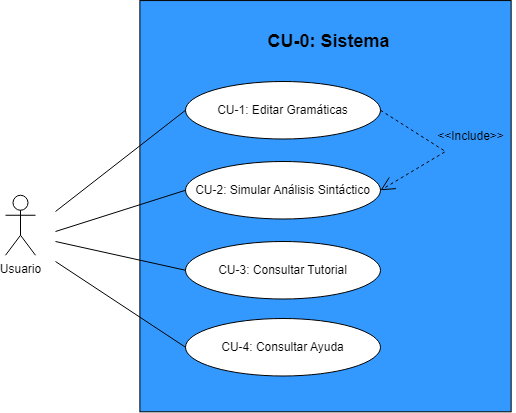
\includegraphics[scale=0.55]{figuras/Cap7/CU0.png}
        \caption{Diagrama de contexto del Sistema}
        \label{fig:diagramaContexto}
    \end{center}
\end{figure}

\subsection{Diagrama de contexto: CU-0. Sistema}

La figura \ref{fig:diagramaContexto}  presenta el diagrama de contexto del sistema, en el cual se identifican los cuatro casos de uso principales que conforman la aplicación. Estos casos de uso son:
\begin{itemize}
    \item \textbf{CU-1. Editar gramática}: corresponde al módulo para la \textit{edición de gramáticas}.
    \item \textbf{CU-2. Simular análisis sintáctico descendente predictivo}: se refiere al módulo que \textit{simula el analizador sintáctico descendente predictivo utilizando gramáticas de contexto libre}.    
    \item \textbf{CU-3. Consultar tutorial}: relacionado con el módulo del \textit{tutorial}.    
    \item \textbf{CU-4. Consultar ayuda}: está relacionado con el módulo de la \textit{ayuda}.
\end{itemize}



La especificación del caso de uso CU-0. Sistema se presenta en la tabla \ref{tabla71}.

\begin{longtable}[htp]{|>{\columncolor[rgb]{0.63,0.79,0.95}}m{6cm} | m{8.5cm} |}
    \caption{Caso de uso: CU-0. Sistema}
    \endfirsthead
    \multicolumn{2}{c}{{\tablename\ \thetable{} -- continua de la página anterior}} \\
    \endhead
    \hline \multicolumn{2}{|r|}{{Continúa en la página siguiente}} \\ \hline
    \endfoot

    \hline
    \endlastfoot

    \hline
    \textbf{Nombre} & \textbf{CU-0. Sistema} (diagrama de contexto).\newline \textbf{Nivel}: 0  \\ 
    \hline
    \textbf{Descripción} &  Proporciona al usuario una visión general de todos los subsistemas que componen la aplicación, registrando todas las interacciones posibles del usuario con estos. \\ \hline                       
    \textbf{Actores} & Usuario \\ \hline

    \textbf{Casos de uso} & \begin{enumerate}
        \item \textbf{CU-1. Editar Gramáticas}: este subsistema se encarga de la edición de gramáticas de contexto libre.                                   
        \item \textbf{CU-2. Simular análisis sintáctico descendente predictivo}: este subsistema se dedica a la simulación del analizador sintáctico descendente predictivo utilizando gramáticas de contexto libre.
        \item \textbf{CU-3. Consultar Tutorial}: proporciona acceso al tutorial de la aplicación.
        \item \textbf{CU-4. Consultar Ayuda}: permite acceder a la ayuda de la aplicación.
    \end{enumerate} 
    \\ \hline
    \textbf{Flujo de eventos principal} & \begin{enumerate}
        \item El usuario inicia sesión en el Sistema.
        \item Se presentan todas las opciones disponibles al usuario.
        \item El usuario selecciona una opción del Sistema.
        \item El Sistema procesa la selección del usuario.
        \item Se proporciona retroalimentación al usuario sobre la selección realizada.
        \item El usuario interactúa con el subsistema seleccionado (por ejemplo, edición de gramáticas, simulación, consulta de tutoriales o ayuda).
        \item El usuario puede guardar su progreso y retornar al menú principal en cualquier momento.
    \end{enumerate} \\ \hline
    \textbf{Flujo de eventos alternativo} & \begin{enumerate}
        \item Ocurre un error durante la inicialización del Sistema.
        \item Se notifica al usuario sobre el error.
        \item El Sistema sugiere posibles soluciones o pasos a seguir para resolver el problema.
        \item Si el error persiste, el Sistema guarda cualquier progreso no guardado previamente y cierra la aplicación de manera segura.
        \item El usuario es redirigido a una página de soporte técnico para obtener asistencia adicional.
    \end{enumerate} 
    \label{tabla71}
\end{longtable}

A continuación, se procederá a detallar todos los casos de uso que conforman las funcionalidades del simulador. Este análisis detallado se realizará de manera sistemática, abordando cada caso de uso general identificado en el diagrama de contexto (figura \ref{fig:diagramaContexto}): CU-1, CU-2, CU-3 y CU-4.


\subsection{CU-1. Editar Gramáticas}

Este caso de uso representa la edición de gramáticas de contexto libre en el sistema. 

  \begin{figure}[H]
       \begin{center} 
 	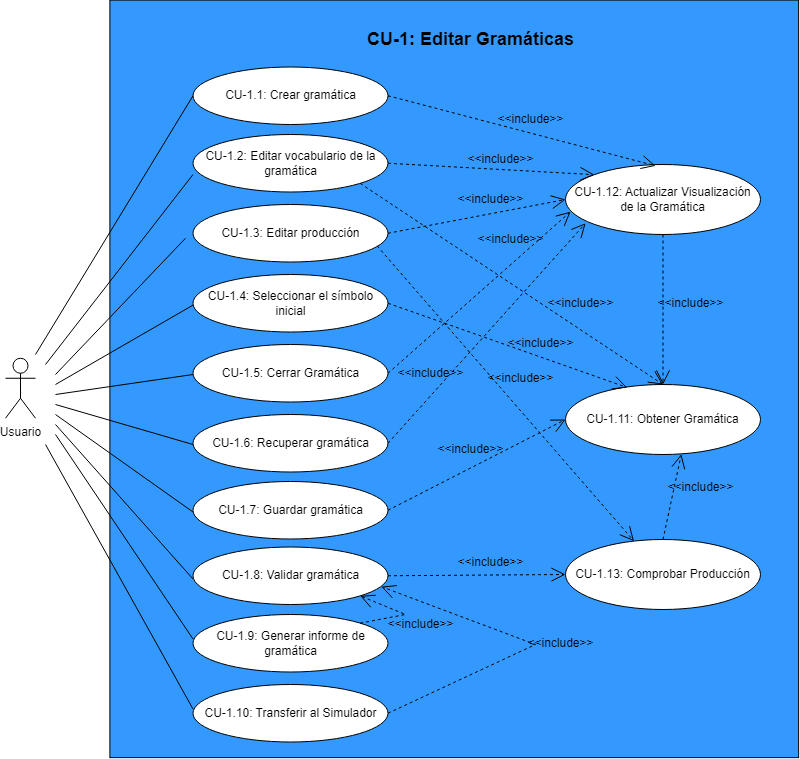
\includegraphics[scale=0.55]{figuras/Cap7/CU1.png}
 	\caption{CU-1: Editar Gramáticas}
 	\label{fig:CU1_EdicionDeGramatica}
      \end{center}
   \end{figure}

La figura \ref{fig:CU1_EdicionDeGramatica} muestra la representación gráfica de este caso de uso, que está formado por los siguientes sub-casos de uso:

 \begin{itemize}
  \item \textbf{CU-1.1. Crear gramática}.
  \item \textbf{CU-1.2. Editar vocabulario de la gramática}.
  \item \textbf{CU-1.3. Editar producción}.
  \item \textbf{CU-1.4. Seleccionar el símbolo inicial}.
  \item \textbf{CU-1.5. Cerrar gramática}.
  \item \textbf{CU-1.6. Recuperar gramática}.
  \item \textbf{CU-1.7. Guardar gramática}.
  \item \textbf{CU-1.8. Validar gramática}.
  \item \textbf{CU-1.9. Generar informe de gramática}.
  \item \textbf{CU-1.10. Transferir al simulador}.
  \item \textbf{CU-1.11. Obtener gramática}.
  \item \textbf{CU-1.12. Actualizar visualización de la gramática}.
  \item \textbf{CU-1.13. Comprobar producción}.
 \end{itemize}


 \begin{longtable}[H]{|>{\columncolor[rgb]{0.63,0.79,0.95}}p{6cm} | p{8.5cm} |}
    \caption{Caso de uso: CU-1. Edición de gramáticas}
    \label{tablaCU1} \\
    \hline
    \textbf{Nombre} & \textbf{CU-1. Editar Gramáticas} \newline \textbf{Nivel}: 1 \\
    \hline
    \textbf{Descripción} & Permite al usuario la creación y edición de gramáticas de contexto libre. \\
    \hline
    \textbf{Actores} & Usuario \\
    \hline
    \textbf{Casos de uso} & 
    \begin{enumerate}
        \item \textbf{CU-1.1. Crear gramática}: permite \textit{crear} una gramática a partir de una producción inicial.
        \item \textbf{CU-1.2. Editar vocabulario de la gramática}: permite \textit{editar} el vocabulario de símbolos ($V_{N}, V_{T}$) de la gramática.
        \item \textbf{CU-1.3. Editar producción}: permite la \textit{edición} de producciones de la gramática.
        \item \textbf{CU-1.4. Seleccionar el símbolo inicial}: permite la \textit{selección} del símbolo inicial de la gramática.
        \item \textbf{CU-1.5. Cerrar gramática}: \textit{cierra} una gramática abierta en el editor.
        \item \textbf{CU-1.6. Recuperar gramática}: \textit{carga} una gramática almacenada en un fichero.
        \item \textbf{CU-1.7. Guardar gramática}: \textit{almacena} una gramática en un fichero.
        \item \textbf{CU-1.8. Validar gramática}: \textit{valida} una gramática de contexto libre.
        \item \textbf{CU-1.9. Generar informe}: \textit{genera} un informe de una gramática de contexto libre.
        \item \textbf{CU-1.10. Transferir al simulador}: \textit{transfiere} una gramática de contexto libre al simulador para simular el análisis sintáctico.
        \item \textbf{CU-1.11. Obtener gramática}: \textit{obtiene} el vocabulario de símbolos ($V_{N}, V_{T}$) así como las producciones de la gramática.
        \item \textbf{CU-1.12. Actualizar visualización de la gramática}: \textit{actualiza} la visualización de la gramática en la interfaz del simulador para permitir al usuario visualizarla a medida que realiza modificaciones en la misma.
        \item \textbf{CU-1.13. Comprobar producción}: \textit{comprueba} si una regla gramatical o producción es correcta o no.
    \end{enumerate} \\
    \hline
    \textbf{Flujo de eventos principal} & 
    \begin{enumerate}
        \item El usuario accede al Sistema.
        \item Se presentan todas las opciones disponibles al usuario.
        \item El usuario selecciona una de las opciones del Sistema.
        \item El Sistema ejecuta la acción correspondiente a la opción seleccionada.
        \item El Sistema proporciona retroalimentación al usuario sobre la acción realizada.
        \item El usuario puede guardar su progreso y retornar al menú principal en cualquier momento.
    \end{enumerate} \\
    \hline
    \textbf{Flujo de eventos alternativo} & 
    \begin{enumerate}
        \item Ocurre un error durante la inicialización del Sistema.
        \item Se notifica al usuario sobre el error.
        \item El Sistema sugiere posibles soluciones o pasos a seguir para resolver el problema.
        \item Si el error persiste, el Sistema guarda cualquier progreso no guardado previamente y cierra la aplicación de manera segura.
        \item El usuario es redirigido a una página de soporte técnico para obtener asistencia adicional.
    \end{enumerate} \\
    \hline
    \textbf{Flujo de eventos alternativo adicional} & La acción representada por el caso de uso CU-1.12 se lleva a cabo de forma continua, sin que lo solicite el usuario. Además, esta acción se ejecuta cada vez que el usuario modifica la gramática utilizando alguno de los casos de uso que implican este sub-caso de uso. \\
    \hline
\end{longtable}


 En las siguientes secciones, se refinará cada uno de los sub-casos de uso que componen el caso de uso CU-1.

\subsubsection{CU-1.1. Crear gramática}

Este caso de uso describe el proceso de creación de una gramática de contexto libre. La figura \ref{fig:CU1.1_CrearGramatica} muestra la representación gráfica del caso de uso, mientras que la tabla \ref{tabla73} presenta su descripción tabular.

 \begin{figure}[H]
       \begin{center} 
 	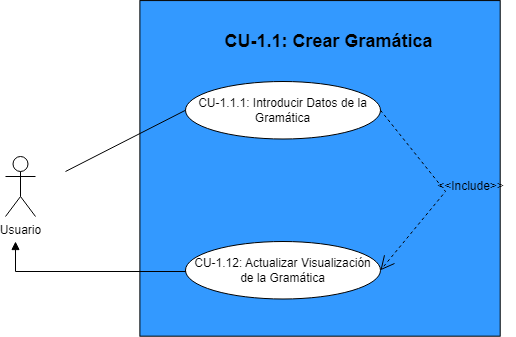
\includegraphics[scale=0.55]{figuras/Cap7/CU11.png}
 	\caption{CU-1.1: Crear gramática}
 	\label{fig:CU1.1_CrearGramatica}
       \end{center}
   \end{figure}

 \begin{longtable}[H]{|>{\columncolor[rgb]{0.63,0.79,0.95}}m{6cm} | m{8.5cm} |}
 \caption{Caso de uso: CU-1.1 Crear gramática} \\
 \endfirsthead
 \multicolumn{2}{c}
 {{ \tablename\ \thetable{} -- continúa de la página anterior}} \\
 \endhead
 \hline \multicolumn{2}{|r|}{{continúa en la página siguiente}} \\ \hline
 \endfoot
 \hline
 \endlastfoot
  \hline
  \textbf{Nombre} & \textbf{CU-1.1 Crear gramática}.\newline \textbf{Nivel}: 2  \\ \hline
  \textbf{Descripción} &  Permite al usuario crear gramáticas de contexto libre. \\ \hline                       
  \textbf{Actores} & Usuario \\ \hline
   \textbf{Casos de uso} & \begin{enumerate}
   \item \textbf{CU-1.1.1 Introducir datos de la gramática}: permite que el usuario \textit{introduzca} los datos de una gramática de contexto libre.
   \item \textbf{CU-1.1.2 Actualizar visualización de la gramática}: \textit{actualiza} la visualización de la gramática en la interfaz del simulador. 
   \end{enumerate} \\ \hline
   \textbf{Flujo de eventos principal} & 
   \begin{enumerate}
   \item El usuario introduce el nombre de la gramática y una descripción de la misma.
    \item Se crea la gramática y se actualiza la visualización en la interfaz.
    \item El usuario recibe una confirmación de la creación exitosa de la gramática.
   \end{enumerate} \\ \hline
   \textbf{Flujo de eventos alternativo} & 
   \begin{enumerate}
        \item Si en el paso 2 se detecta algún error durante la actualización de la visualización:
        \begin{enumerate}
        \item Se informa al usuario del error producido.
        \item El sistema proporciona posibles soluciones o pasos a seguir.
        \end{enumerate}
    \end{enumerate} 
   \label{tabla73}
 \end{longtable}

El caso de uso \textit{CU-1.1.1 Introducir datos de la gramática} no requiere un refinamiento adicional debido a su simplicidad. Este caso de uso se encarga de solicitar al usuario el nombre y la descripción de la gramática, excluyendo símbolos y producciones, para posteriormente incorporarlos en la definición de la gramática.

\subsubsection{CU-1.2. Editar vocabulario de la gramática}

Este caso de uso describe el proceso de edición del vocabulario de la gramática, incluyendo tanto los símbolos terminales como los no terminales. La figura \ref{fig:CU1.2} muestra la representación gráfica del caso de uso, mientras que la tabla \ref{tabla74} presenta su descripción tabular.

  \begin{figure}[H]
       \begin{center} 
 	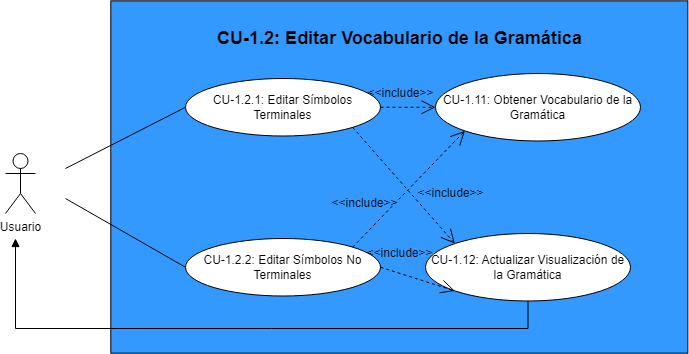
\includegraphics[scale=0.55]{figuras/Cap7/CU12.png}
 	\caption{CU-1.2: Editar vocabulario de la gramática}
 	\label{fig:CU1.2}
       \end{center}
   \end{figure}

 \begin{longtable}[H]{|>{\columncolor[rgb]{0.63,0.79,0.95}}m{6cm} | m{8.5cm} |}
 \caption{Caso de uso: CU-1.2 Editar vocabulario de la gramática} \\
 \endfirsthead
 \multicolumn{2}{c}
 {{ \tablename\ \thetable{} -- continúa de la página anterior}} \\
 \endhead
 \hline \multicolumn{2}{|r|}{{continúa en la página siguiente}} \\ \hline
 \endfoot
 \hline
 \endlastfoot
 \hline
 \textbf{Nombre} & \textbf{CU-1.2 Editar vocabulario de la gramática}.\newline \textbf{Nivel}: 2  \\ \hline
 \textbf{Descripción} &  Permite al usuario editar el vocabulario ($V_{N}, V_{T}$) de la gramática. \\ \hline
 \textbf{Actores} & Usuario \\ \hline
  \textbf{Casos de uso} & 
     \begin{enumerate}
     \item \textbf{CU-1.2.1. Editar símbolos terminales}: permite que el usuario \textit{introduzca o modifique} el conjunto de símbolos terminales de la gramática.
     \item \textbf{CU-1.2.2. Editar símbolos no terminales}: permite que el usuario \textit{introduzca o modifique} el conjunto de símbolos no terminales de la gramática. 
     \item \textbf{CU-1.11. Obtener gramática}: \textit{obtiene} el vocabulario de símbolos ($V_{N}, V_{T}$) así como las producciones de la gramática.
     \item \textbf{CU-1.12. Actualizar vi\-sua\-li\-za\-ción de la gramática}: \textit{actualiza} la visualización de la gramática en la interfaz del simulador.
     \end{enumerate} \\ \hline
  \textbf{Flujo de eventos principal} & 
     \begin{enumerate}
     \item El usuario elige entre alguna de las opciones disponibles:
         \begin{enumerate}
         \item Introducir el conjunto de símbolos terminales de la   gramática y se comprueba si son correctos.
         \item Introducir el conjunto de símbolos no terminales de la  gramática y se comprueba si son correctos.     
         \end{enumerate} 
     \end{enumerate} \\ \hline                     
  \textbf{Flujo de eventos alternativo} & Si durante la opción o función 1, se detecta que alguno de los símbolos terminales introducido no es co\-rrec\-to:
     \begin{enumerate}
     \item Se informa al usuario del error producido.
     \item Se pide al usuario que reintroduzca el símbolo terminal que produjo el error.
     \end{enumerate}\\ \hline              
   \textbf{Flujo de eventos alternativo} & Si durante la opción o función 2, se detecta que alguno de los símbolos no terminales introducido no es co\-rrec\-to:
     \begin{enumerate}
     \item Se informa al usuario del error producido.
     \item Se pide al usuario que reintroduzca el símbolo no terminal que produjo el error.
     \end{enumerate}         
   \label{tabla74}
 \end{longtable}

 Los casos de uso \textit{CU-1.2.1 Editar símbolos terminales} y \textit{CU-1.2.2 Editar símbolos no terminales} no se refinarán más, puesto que son casos de uso bastante sencillos y que pueden ser fácilmente traducidos a una implementación posterior sin necesidad de ser refinados.

 El caso de uso CU-1.2.1 mostrará al usuario una ventana para \textit{introducir} o \textit{modificar} (en el caso de que ya los haya introducido) todos los símbolos terminales de la gramática, mientras que el caso de uso CU-1.2.2 permitirá modificar los no terminales.

 \subsubsection{CU-1.3. Editar producción}

 Este caso de uso representa la edición de una producción de una gramática. En la figura \ref{fig:CU13} se muestra la representación gráfica del caso de uso y en la tabla \ref{tabla75} se muestra su representación tabular.

 \begin{figure}[H]
       \begin{center} 
 	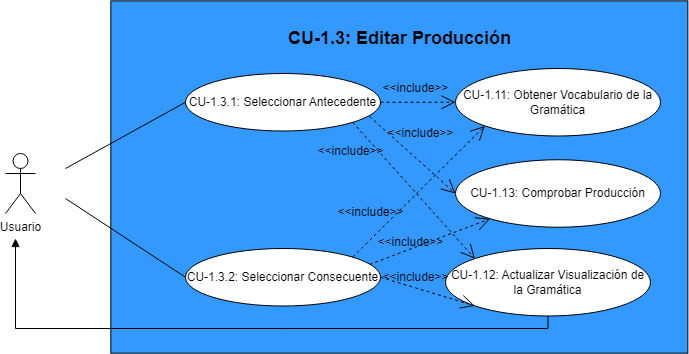
\includegraphics[scale=0.55]{figuras/Cap7/CU13.png}
 	\caption{CU-1.3: Editar producción}
 	\label{fig:CU13}
       \end{center}
 \end{figure}


 \begin{longtable}[H]{|>{\columncolor[rgb]{0.63,0.79,0.95}}m{6cm} | m{8.5cm} |}
 \caption{Caso de uso: CU-1.3: Editar producción} \\
 \endfirsthead
 \multicolumn{2}{c}
 {{ \tablename\ \thetable{} -- continúa de la página anterior}} \\
 \endhead
 \hline \multicolumn{2}{|r|}{{continúa en la página siguiente}} \\ \hline
 \endfoot
 \hline
 \endlastfoot

  \hline
  \textbf{Nombre} & \textbf{CU-1.3 Editar producción}.\newline \textbf{Nivel}: 2  \\ \hline
  \textbf{Descripción} & Permite al usuario editar una producción de la gramática de contexto libre.\\ \hline
  \textbf{Actores} & Usuario \\ \hline
  \textbf{Casos de uso} & 
     \begin{enumerate}
     \item \textbf{CU-1.3.1 Seleccionar antecedente}: permite que el usuario \textit{modifique}  el antecedente de una producción.
     \item \textbf{CU-1.3.2 Seleccionar consecuente}: permite que el usuario \textit{modifique}  el consecuente de una producción.
     \item \textbf{CU-1.11. Obtener gramática}: \textit{obtiene} el vocabulario de símbolos ($V_{N}, V_{T}$) así como las producciones de la gramática.
     \item \textbf{CU-1.12. Actualizar vi\-sua\-li\-za\-ción de la gramática}: \textit{actualiza} la visualización de la gramática en la interfaz del simulador.
     \item \textbf{CU-1.13 Comprobar producción}: \textit{comprueba} si una producción es correcta.
     \end{enumerate} \\ \hline
      \textbf{Flujo de eventos principal} & 
         \begin{enumerate}
         \item El usuario \textit{selecciona} el antecedente o el consecuente (o  ambos) de la producción que desea crear o modificar (en caso de que en CU-1 el usuario hubiera seleccionado alguna producción que ya existía).
         \item El usuario \textit{modifica} el antecedente o el consecuente (o ambos).
         \item Se \textit{comprueba} si la producción modificada es correcta.
         \end{enumerate} \\ \hline
  \textbf{Flujo de eventos alternativo} & Si no existe ningún símbolo en el vocabulario de la gramática (o solamente existe uno de los conjuntos de símbolos: terminales o no terminales) o bien alguno de los símbolos posee un error, se procede como sigue:
     \begin{enumerate}
     \item Se \textit{informa} al usuario del evento y se le pide que introduzca o modifique el conjunto de símbolos de la gramática.
     \end{enumerate} \\ \hline          
  \textbf{Flujo de eventos alternativo} & Si se produce algún fallo durante el paso 2, se procede como sigue:
     \begin{enumerate}
     \item Se \textit{informa} al usuario del error producido.
     \item Se \textit{deshacen} los cambios re\-a\-li\-zados por el usuario en la producción.
     \end{enumerate} \\ \hline              
   \textbf{Flujo de eventos alternativo} & Si se comprueba la producción resultante y esta no es correcta, se procede como sigue:
   \begin{enumerate}
   \item Se \textit{informa} al usuario del error (diciendo además si está en el antecedente,  en el consecuente o en ambos) y el motivo del mismo.
   \item Se \textit{pide} al usuario que corrija el e\-rror.              \end{enumerate}
   \label{tabla75}
 \end{longtable}

 Los casos de uso \textit{CU-1.3.1 Seleccionar antecedente} y \textit{CU-1.3.2 Seleccionar consecuente} no se refinarán más, puesto que son casos de uso bastante sencillos y que pueden ser fácilmente traducidos a una implementación posterior sin necesidad de ser refinados.

 El caso de uso CU-1.3.1 mostrará un diálogo al usuario que le permita seleccionar el antecedente de la producción de entre los símbolos no terminales que introdujo (mediante el caso de uso 1.2).

 El caso de uso CU-1.3.2, por su parte, permitirá al usuario modificar el consecuente de la producción (re\-a\-li\-zando acciones análogas a la del caso de uso 1.3.1).

 \subsubsection{CU-1.4. Seleccionar el símbolo inicial}

 Este caso de uso representa la selección del símbolo inicial de la gramática. En la figura \ref{fig:CU14} se muestra la representación gráfica del caso de uso y en la  tabla \ref{tabla76} se muestra su representación tabular.

   \begin{figure}[H]
       \begin{center} 
 	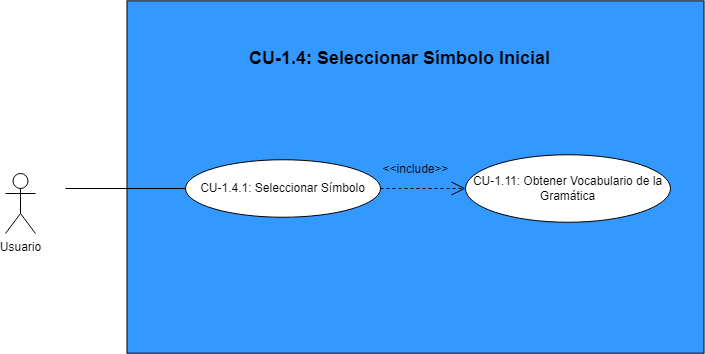
\includegraphics[scale=0.55]{figuras/Cap7/CU14.png}
 	\caption{CU-1.4: Seleccionar el símbolo inicial}
 	\label{fig:CU14}
       \end{center}
   \end{figure}


 \begin{longtable}[H]{|>{\columncolor[rgb]{0.63,0.79,0.95}}m{6cm} | m{8.5cm} |}
 \caption{Caso de uso: CU-1.4 Seleccionar el símbolo inicial} \\
 \endfirsthead
 \multicolumn{2}{c}
 {{ \tablename\ \thetable{} -- continúa de la página anterior}} \\
 \endhead
 \hline \multicolumn{2}{|r|}{{continúa en la página siguiente}} \\ \hline
 \endfoot
 \hline
 \endlastfoot
  \hline
  \textbf{Nombre} & \textbf{CU-1.4 Seleccionar el símbolo inicial}.\newline \textbf{Nivel}: 2  \\ \hline
  \textbf{Descripción} & Permite al usuario seleccionar el símbolo inicial 
  de la gramática de contexto libre.\\ \hline
  \textbf{Actores} & Usuario \\ \hline 
  \textbf{Casos de uso} & 
     \begin{enumerate}
     \item \textbf{CU-1.4.1 Seleccionar símbolo}: permite que el usuario \textit{seleccione} un  símbolo inicial de entre el conjunto de símbolos no terminales de la gramática.
     \item \textbf{CU-1.11. Obtener gramática}: \textit{obtiene} el vocabulario de símbolos ($V_{N}, V_{T}$) así como las producciones de la gramática. 
     \end{enumerate} \\ \hline
 \textbf{Flujo de eventos principal} & 
     \begin{enumerate}
     \item Se \textit{obtienen} los símbolos no terminales de la gramática.
     \item Se \textit{muestra} al usuario un diálogo para seleccionar el símbolo inicial de la gramática.
     \item El usuario \textit{selecciona} un símbolo para que sea el inicial. 
     \item Se \textit{comprueba} la producción en la que el símbolo aparece como antecedente.
     \item Se \textit{asigna} dicho símbolo como símbolo inicial.
     \end{enumerate}\\ \hline                 
  \textbf{Flujo de eventos alternativo} & Si se produce algún fallo durante el paso 3, se procede como sigue:
    \begin{enumerate}
    \item Se \textit{informa} al usuario del error producido.
    \item Se \textit{termina} la acción de seleccionar símbolo inicial.
    \end{enumerate}  \\ \hline           
  \textbf{Flujo de eventos alternativo} & Si se produce algún fallo durante el paso 4, se procede como sigue:
  \begin{enumerate}
  \item Se \textit{informa} al usuario de que la producción en la que el símbolo aparece en  el antecedente no es correcta.
  \item Se \textit{permite} al usuario modificar dicha producción.
  \item Se \textit{reanuda} el paso 4, permitiendo al usuario continuar con la asignación de símbolo inicial. 
  \end{enumerate} \\ \hline            
   \textbf{Flujo de eventos alternativo} & Si se producen errores en el paso 5, se procede como sigue:
   \begin{enumerate}
   \item Se \textit{informa} al usuario del error.
   \item Se \textit{reintenta} asignar el símbolo, abortando la acción actual en caso de que  siga siendo imposible dicha asignación.
   \end{enumerate}
  \label{tabla76}
 \end{longtable}

 El caso de uso \textit{CU-1.4.1 Seleccionar símbolo} no se refinará más, puesto que se trata de un caso de uso bastante sencillo y que puede ser fácilmente traducido a una implementación posterior sin necesidad de ser refinados. Este caso de uso simplemente se encargará de mostrar, una vez obtenidos los símbolos no terminales de la gramática, un diálogo que permita seleccionar el símbolo inicial (de entre todos los símbolos no terminales que posee la gramática).
 
  \subsubsection{CU-1.5. Cerrar gramática}

 Este caso de uso se encarga de cerrar la gramática seleccionada por el usuario (con una posterior actualización de la vista de la gramática).

 Este caso de uso no se refinará más, puesto que el proceso de cierre de la gramática es inmediato y evidente.

 \subsubsection{CU-1.6. Recuperar gramática}

 Este caso de uso representa la recuperación de una gramática desde un fichero. En la figura \ref{fig:CU16} se muestra la representación gráfica del caso de uso y en la tabla \ref{tabla77} se muestra su representación tabular.

  \begin{figure}[H]
       \begin{center} 
 	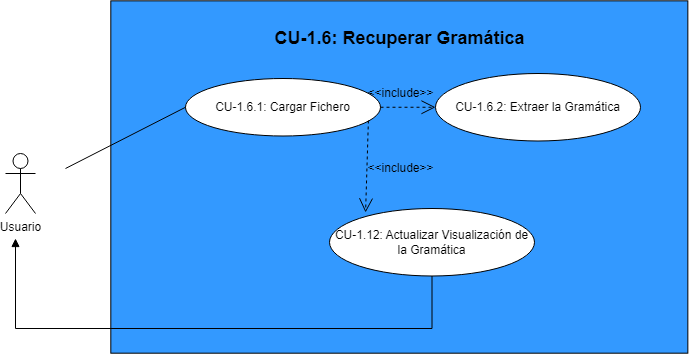
\includegraphics[scale=0.55]{figuras/Cap7/CU16.png}
 	\caption{CU-1.6: Recuperar gramática}
 	\label{fig:CU16}
       \end{center}
   \end{figure}

 \begin{longtable}[H]{|>{\columncolor[rgb]{0.63,0.79,0.95}}m{6cm} | m{8.5cm} |}
 \caption{Caso de uso: CU-1.6 Recuperar gramática} \\
 \endfirsthead
 \multicolumn{2}{c}
 {{ \tablename\ \thetable{} -- continúa de la página anterior}} \\
 \endhead
 \hline \multicolumn{2}{|r|}{{continúa en la página siguiente}} \\ \hline
 \endfoot
 \hline
 \endlastfoot
  \hline
  \textbf{Nombre} & \textbf{CU-1.6 Recuperar gramática}.\newline \textbf{Nivel}: 2  \\ \hline
  \textbf{Descripción} & Permite al usuario recuperar una gramática de un fichero.\\ \hline
  \textbf{Actores} & Usuario \\ \hline
  \textbf{Casos de uso} & 
     \begin{enumerate}
     \item \textbf{CU-1.6.1 Cargar fichero}: \textit{carga} un fichero que contiene una gramática.
     \item \textbf{CU-1.6.2 Extraer la gramática}:  \textit{extrae} la gramática contenida en el fichero recuperado.
     \item \textbf{CU-1.12. Actualizar visualización de la gramática}: \textit{actualiza} la visualización de la gramática en la interfaz del simulador.
     \end{enumerate} \\ \hline
  \textbf{Flujo de eventos principal} & 
     \begin{enumerate}
     \item El usuario \textit{selecciona} el fichero que contiene la gramática que desea cargar.
     \item Se \textit{extrae} la gramática del fichero.
     \item Se \textit{carga} la gramática en el editor (creando toda la estructura de la gramática y actualizando la vista de la gramática pertinente).
     \end{enumerate}\\ \hline
  \textbf{Flujo de eventos alternativo} & Si se produce algún fallo durante el paso 1, se procede como sigue: 
     \begin{enumerate}
     \item Se \textit{informa} al usuario de que no ha podido seleccionar ningún fichero. 
     \item Se \textit{termina} la acción de recuperar gramática.
     \end{enumerate}  \\ \hline
  \textbf{Flujo de eventos alternativo} & Si se produce algún fallo durante el paso 2, se procede como sigue:
     \begin{enumerate}
     \item Se \textit{informa} al usuario de que la gramática no pudo ser extraída o cargada en  el simulador, debido a posibles problemas en la estructura del archivo.
     \item Se \textit{termina} la acción de recuperar gramática.
     \end{enumerate} \\ \hline          
   \textbf{Flujo de eventos alternativo} & Si se produce algún fallo durante el paso 3, se procede como sigue:
         \begin{enumerate}
         \item Se \textit{informa} al usuario de que la gramática ha podido ser extraída pero no se puede cargar en el editor.
         \item Se \textit{termina} la acción de recuperar gramática.
         \end{enumerate}
   \label{tabla77}
 \end{longtable}

 Los casos de uso \textit{CU-1.6.1 Cargar fichero} y \textit{CU-1.6.2 Extraer gramática} no se refinarán más, puesto que son casos de uso bastante sencillos y que pueden ser fácilmente traducidos a una implementación posterior sin necesidad de ser refinados.

 \subsubsection{CU-1.7. Guardar gramática}

 Este caso de uso representa el almacenamiento de una gramática. En la figura \ref{fig:CU17} se muestra la representación gráfica del caso de uso y en la tabla \ref{tabla78} se muestra su representación tabular. 

   \begin{figure}[H]
       \begin{center} 
 	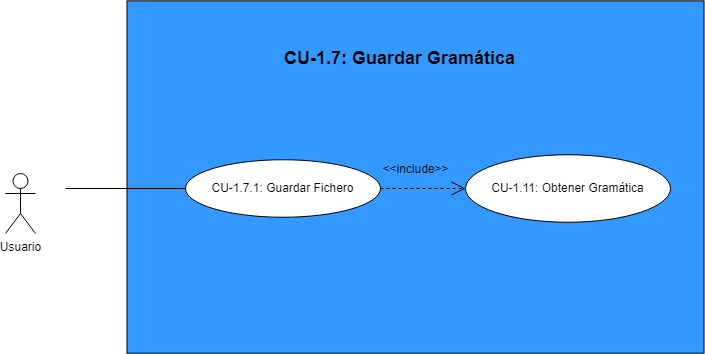
\includegraphics[scale=0.55]{figuras/Cap7/CU17.png}
 	\caption{CU-1.7: Guardar gramática}
 	\label{fig:CU17}
       \end{center}
   \end{figure}
  
   \newpage

 \begin{longtable}[H]{|>{\columncolor[rgb]{0.63,0.79,0.95}}m{6cm} | m{8.5cm} |} 
 \caption{Caso de uso: CU-1.7 Guardar gramática} \\
 \endfirsthead
 \multicolumn{2}{c}
 {{ \tablename\ \thetable{} -- continúa de la página anterior}} \\
 \endhead
 \hline \multicolumn{2}{|r|}{{continúa en la página siguiente}} \\ \hline
 \endfoot
 \hline
 \endlastfoot

  \hline
  \textbf{Nombre} & \textbf{CU-1.7 Guardar gramática}.\newline \textbf{Nivel}: 2  \\ \hline
   \textbf{Descripción} & Permite al usuario guardar una gramática de un fichero.\\ \hline                    
  \textbf{Actores} & Usuario \\ \hline
  \textbf{Casos de uso} & 
     \begin{enumerate}
     \item \textbf{CU-1.7.1 Guardar fichero}: \textit{guarda} en un fichero la gramática creada.
     \item \textbf{CU-1.11. Obtener gramática}: \textit{obtiene} el vocabulario de símbolos ($V_{N}, V_{T}$) así como las producciones de la gramática.
     \end{enumerate} \\ \hline
  \textbf{Flujo de eventos principal} & 
     \begin{enumerate}
     \item El usuario \textit{selecciona} el fichero en el que desea guardar la gramática.
     \item Se \textit{guarda} la gramática en un fichero (con el formato especificado en el capítulo anterior).
     \end{enumerate}\\ \hline
  \textbf{Flujo de eventos alternativo} & Si se produce algún fallo durante el paso 1, se procede como sigue:
     \begin{enumerate}
     \item Se \textit{informa} al usuario de que no ha podido seleccionar crear el fichero.
     \item Se \textit{termina} la acción de guardar gramática.
     \end{enumerate}  \\ \hline
  \textbf{Flujo de eventos alternativo} & Si se produce algún fallo durante el paso 2, se procede como sigue:
     \begin{enumerate}
     \item Se \textit{informa} al usuario de que la gramática no pudo ser guardada.
     \item Se \textit{termina} la acción de guardar gramática.
     \end{enumerate} 
   \label{tabla78}
 \end{longtable}

 El caso de uso \textit{CU-1.7.1 Guardar fichero} no se refinará más, puesto que se trata de un proceso simple que puede ser fácilmente traducido a una implementación posterior sin necesidad de ser refinado más.

 \subsubsection{CU-1.8. Validar gramática}

 Este caso de uso representa la validación de una gramática. En la figura \ref{fig:CU18} se muestra la representación gráfica del caso de uso y en la tabla \ref{tabla79} se muestra su representación tabular.

 \begin{figure}[H]
       \begin{center} 
 	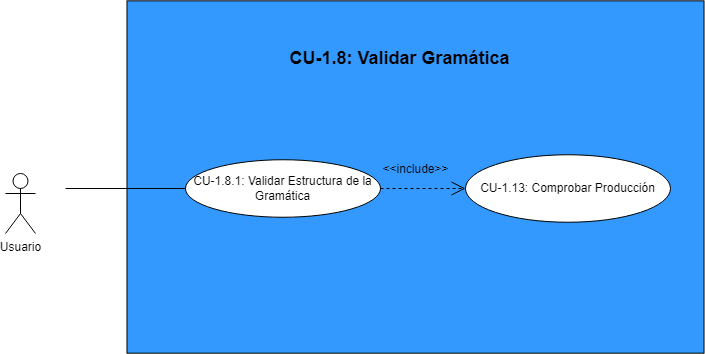
\includegraphics[scale=0.55]{figuras/Cap7/CU18.png}
 	\caption{CU-1.8: Validar gramática}
 	\label{fig:CU18}
       \end{center}
   \end{figure}
  
   \newpage

 \begin{longtable}[H]{|>{\columncolor[rgb]{0.63,0.79,0.95}}m{6cm} | m{8.5cm} |}
 \caption{Caso de uso: CU-1.8 Validar gramática} \\
 \endfirsthead
 \multicolumn{2}{c}
 {{ \tablename\ \thetable{} -- continúa de la página anterior}} \\
 \endhead
 \hline \multicolumn{2}{|r|}{{continúa en la página siguiente}} \\ \hline
 \endfoot
 \hline
 \endlastfoot
  \hline
  \textbf{Nombre} & \textbf{CU-1.8 Validar gramática}.\newline \textbf{Nivel}: 2  \\ \hline
  \textbf{Descripción} & Permite al usuario validar una gramática de contexto libre.\\ \hline
  \textbf{Actores} & Usuario \\ \hline
  \textbf{Casos de uso} & 
     \begin{enumerate}
     \item \textbf{CU-1.8.1 Validar estructura de la gramática}: \textit{valida} la estructura  de la gramática, formada por el conjunto de producciones, símbolos (\textit{terminales} y \textit{no terminales}) y símbolo inicial.
     \item \textbf{CU-1.12 Comprobar producción}: \textit{comprueba} si una producción es correcta.
     \end{enumerate} \\ \hline                             
  \textbf{Flujo de eventos principal} & 
     \begin{enumerate}
     \item Se \textit{obtiene} todo el vocabulario de la gramática a ser validada. 
     \item Se \textit{comprueban} todas las producciones que componen la gramática.
     \item Se \textit{informa} al usuario acerca del resultado del la validación.
     \end{enumerate}\\ \hline                 
  \textbf{Flujo de eventos alternativo} & Si se produce algún fallo durante el paso 1, se procede como sigue:
     \begin{enumerate}
     \item Se \textit{informa} al usuario de que no ha podido obtener el vocabulario de  la gramática.
     \item Se \textit{termina} la acción de validar gramática.
     \end{enumerate}  \\ \hline          
  \textbf{Flujo de eventos alternativo} & Si se produce algún fallo durante el paso 2, se procede como sigue:
     \begin{enumerate}
     \item Se \textit{informa} al usuario de que no se han podido comprobar las producciones de  la gramática.
     \item Se \textit{termina} la acción de validar gramática.
     \end{enumerate} \\ \hline         
  \textbf{Flujo de eventos excepcional} & Si durante la ejecución del paso 2, alguna producción comprobada posee e\-rro\-res (esto excluye cualquier error de funcionamiento, des\-cri\-to en el flujo alternativo anterior), se procede como sigue:
     \begin{enumerate}
     \item El \textit{resultado} de la validación será insatisfactorio.
     \end{enumerate}
   \label{tabla79}
 \end{longtable}

 El caso de uso \textit{CU-1.8.1 Validar estructura de la gramática} no se refinará más, puesto que es un proceso simple que puede ser fácilmente traducido a una implementación posterior sin necesidad de ser refinado más.

 \subsubsection{CU-1.9. Generar informe de gramática}
 
 Este caso de uso representa la generación de un informe de una gramática. En la figura \ref{fig:CU19} se muestra la representación gráfica del caso de uso y en la  tabla \ref{tabla710} se muestra su representación tabular.

  \begin{figure}[H]
       \begin{center} 
 	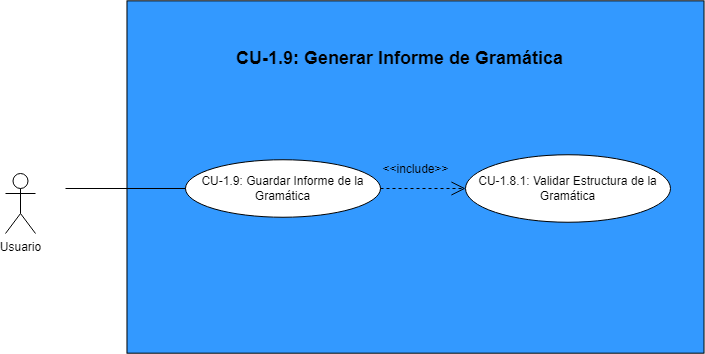
\includegraphics[scale=0.55]{figuras/Cap7/CU19.png}
 	\caption{CU-1.9: Generar informe de gramática}
 	\label{fig:CU19}
       \end{center}
   \end{figure}

 \begin{longtable}[H]{|>{\columncolor[rgb]{0.63,0.79,0.95}}m{6cm} | m{8.5cm} |}
 \caption{Caso de uso: CU-1.9 Generar informe de gramática} \\
 \endfirsthead
 \multicolumn{2}{c}
 {{ \tablename\ \thetable{} -- continúa de la página anterior}} \\
 \endhead
 \hline \multicolumn{2}{|r|}{{continúa en la página siguiente}} \\ \hline
 \endfoot
 \hline
 \endlastfoot
  \hline
  \textbf{Nombre} & \textbf{CU-1.9 Generar informe de gramática}. \newline \textbf{Nivel}: 2  \\ \hline
  \textbf{Descripción} & Permite al usuario generar un informe de una gramática.\\ \hline                       
  \textbf{Actores} & Usuario \\ \hline
  \textbf{Casos de uso} & 
     \begin{enumerate}
     \item \textbf{CU-1.9.1 Guardar informe de la gramática}: \textit{guarda} un fichero que  contiene el informe de la gramática.
     \item \textbf{CU-1.8.1 Validar estructura de la gramática}: \textit{valida} la estructura  de la gramática, formada por el conjunto de producciones y símbolos (\textit{terminales} y \textit{no terminales}).
     \end{enumerate} \\ \hline
 
  \textbf{Flujo de eventos principal} & 
         \begin{enumerate}
         \item Se re\-a\-li\-za una \textit{validación} de la estructura de la gramática, para así  comprobar si la gramática es co\-rrec\-ta.
         \item Se \textit{genera} un informe de la gramática, según lo especificado en \textit{RI- INF-1}.
         \end{enumerate}\\ \hline             
  \textbf{Flujo de eventos alternativo} & Si se produce algún fallo durante el paso 1, se procede como sigue:
     \begin{enumerate}
     \item Se \textit{informa} al usuario que no ha podido generar el informe de la gramática.
     \item Se \textit{termina} la acción de generar informe de gramática.
     \end{enumerate}   \\ \hline              
  \textbf{Flujo de eventos alternativo} & Si se produce algún fallo durante el paso 2, se procede como sigue:
     \begin{enumerate}
     \item Se \textit{informa} al usuario de que el informe no ha podido ser guardado.
     \item Se \textit{termina} la acción de generar informe de gramática.
     \end{enumerate}  \\ \hline
  \textbf{Flujo de eventos excepcional} & Si durante la ejecución del paso 1, se detecta que la gramática no es válida, puesto que posee errores (esto excluye cualquier error de funcionamiento, descrito en el flujo alternativo anterior), se procede como sigue:
     \begin{enumerate}
     \item Se \textit{aborta} la generación del informe.
     \item Se \textit{informa} al usuario de que la gramática contiene errores.
     \end{enumerate}
   \label{tabla710}
 \end{longtable}

 El caso de uso \textit{CU-1.9.1 Guardar informe de la gramática} no se refinará más, puesto que es un \textbf{proceso simple} que puede ser fácilmente traducido a una implementación posterior sin necesidad de ser refinado.

 \subsubsection{CU-1.10. Transferir al simulador}

 Este caso de uso representa la transferencia de una gramática al simulador. En la figura \ref{fig:CU110} se muestra la representación gráfica del caso de uso y en la tabla \ref{tabla711} se muestra su representación tabular.

 \begin{figure}[H]
       \begin{center} 
 	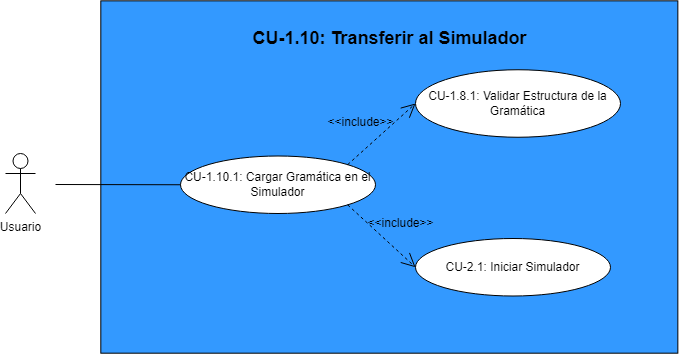
\includegraphics[scale=0.55]{figuras/Cap7/CU110.png}
 	\caption{CU-1.10: Transferir al simulador}
 	\label{fig:CU110}
       \end{center}
   \end{figure}

 \begin{longtable}[H]{|>{\columncolor[rgb]{0.63,0.79,0.95}}m{6cm} | m{8.5cm} |}
 \caption{Caso de uso: CU-1.10 Transferir al simulador} \\
 \endfirsthead
 \multicolumn{2}{c}
 {{ \tablename\ \thetable{} -- continúa de la página anterior}} \\
 \endhead
 \hline \multicolumn{2}{|r|}{{continúa en la página siguiente}} \\ \hline
 \endfoot
 \hline
 \endlastfoot
  \hline
  \textbf{Nombre} & \textbf{CU-1.10 Transferir al simulador}.\newline \textbf{Nivel}: 2  \\ \hline
  \textbf{Descripción} & Permite al usuario transferir una gramática al simulador para simular un método de  análisis sintáctico.\\ \hline
  \textbf{Actores} & Usuario \\ \hline
  \textbf{Casos de uso} & 
     \begin{enumerate}
     \item \textbf{CU-1.10.1 Cargar gramática en el simulador}: \textit{carga} la gramática en  el si\-mu\-la\-dor.
     \item \textbf{CU-1.8.1 Validar estructura de la gramática}: \textit{valida} la estructura  de la gramática, formada por el conjunto de producciones y símbolos (\textit{terminales} y \textit{no terminales}).
     \item \textbf{CU-2.1. Iniciar el simulador}: \textit{i\-ni\-cia\-li\-za} el simulador y  transfiere la gramática, o simplemente carga la gramática en el simulador (en el caso de que este ya se encuentre ini\-cia\-li\-zado previamente).
     \end{enumerate} \\ \hline                             
  \textbf{Flujo de eventos principal} & 
     \begin{enumerate}
     \item Se \textit{re\-a\-li\-za} una validación de la estructura de la gramática, para así  comprobar si la gramática es co\-rre\-cta.
     \item Se \textit{transfiere} la gramática al si\-mu\-la\-dor y se ini\-cia\-li\-za este (en caso de que no se haya iniciado anteriormente al transferir otra gramática)
     \end{enumerate}\\ \hline
  \textbf{Flujo de eventos alternativo} & Si se produce algún fallo durante el paso 1, se procede como sigue:
     \begin{enumerate}
     \item Se \textit{informa} al usuario de que no ha podido validar la gramática.
     \item Se \textit{termina} la acción de transferir al si\-mu\-la\-dor.
     \end{enumerate}  \\ \hline              
  \textbf{Flujo de eventos alternativo} & Si se produce algún fallo durante el paso 2, se procede como sigue:
     \begin{enumerate}
     \item Se \textit{informa} al usuario de que no se ha podido transferir la gramática.
     \item Se \textit{termina} la acción de transferir al si\-mu\-la\-dor.
     \end{enumerate}  \\ \hline             
  \textbf{Flujo de eventos excepcional} & Si durante la ejecución del paso 1, se detecta que la gramática no es válida, puesto que posee errores (esto excluye cualquier error de funcionamiento, des\-cri\-to en el flujo alternativo anterior), se procede como sigue: 
     \begin{enumerate}
     \item Se \textit{aborta} la transferencia de la gramática.
     \item Se \textit{informa} al usuario de que la gramática contiene errores (no es una gramática válida).
     \end{enumerate}
   \label{tabla711}
 \end{longtable}

 El caso de uso \textit{CU-1.10.1 Cargar gramática en el simulador} no se refinará más, puesto que se trata de un proceso simple, que puede ser fácilmente traducido a una implementación posterior sin necesidad de ser refinado.

 \subsubsection{CU-1.11. Obtener gramática}

 Este caso de uso se encarga de obtener el vocabulario de la gramática $ (V_{N}, V_{T}) $, así como todo el conjunto de producciones y el símbolo inicial.

 Se trata de un proceso bastante sencillo, pero que es utilizado en los demás casos de uso cada vez que se desea obtener la estructura de una gramática. Este caso de uso será directamente traducido a una implementación sin ser preciso re\-a\-li\-zar un refinamiento más exhaustivo.

 \subsubsection{CU-1.12. Actualizar visualización}

 Este caso de uso representa la actualización de la visualización de una gramática. Cabe destacar que este caso de uso no es invocado directamente por el usuario, sino que el propio Sistema actualiza la vista de la gramática automáticamente, a medida que esta sufre alguna modificación (a partir de aquellos casos de uso que incluyen el comportamiento de este caso de uso). En la figura \ref{fig:CU112} se muestra la representación gráfica del caso de uso y en la  tabla \ref{tabla712} se muestra su representación tabular.

  \begin{figure}[H]
       \begin{center} 
 	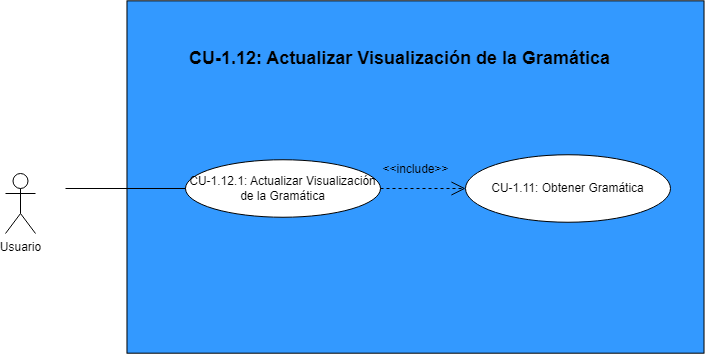
\includegraphics[scale=0.55]{figuras/Cap7/CU112.png}
 	\caption{CU-1.12: Actualizar visualización de la gramática}
 	\label{fig:CU112}
       \end{center}
   \end{figure}

 \begin{longtable}[H]{|>{\columncolor[rgb]{0.63,0.79,0.95}}m{6cm} | m{8.5cm} |}
 \caption{Caso de uso: CU-1.12 Actualizar visualización de la gramática} \\
 \endfirsthead
 \multicolumn{2}{c}
 {{ \tablename\ \thetable{} -- continúa de la página anterior}} \\
 \endhead
 \hline \multicolumn{2}{|r|}{{continúa en la página siguiente}} \\ \hline
 \endfoot
 \hline
 \endlastfoot
  \hline
  \textbf{Nombre} & \textbf{CU-1.12 Actualizar visualización de la gramática}.\newline \textbf{Nivel}: 2  \\ \hline
  \textbf{Descripción} & Permite al usuario visualizar la gramática a medida que la va construyendo.\\ \hline                       
  \textbf{Actores} & Usuario \\ \hline
  \textbf{Casos de uso} & 
     \begin{enumerate}
     \item \textbf{CU-1.12.1 Actualizar vi\-sua\-li\-za\-ción de la gramática}: \textit{ac\-tua\-li\-za} la vi\-sua\-li\-za\-ción de la gramática en el editor, a medida que esta sufre alguna modificación en su estructura (producciones y símbolos).
     \item \textbf{CU-1.11. gramática}: \textit{obtiene} el vocabulario de símbolos ($V_{N}, V_{T}$) así como las producciones de la gramática.
     \end{enumerate} \\ \hline
  \textbf{Flujo de eventos principal} & 
     \begin{enumerate}
     \item Se \textit{obtiene} el vocabulario de la gramática.               \item Se \textit{actualiza} la vista de la gramática en el editor de gramáticas.
     \end{enumerate}\\ \hline                     
  \textbf{Flujo de eventos alternativo} & Si se produce algún fallo durante el paso 1, se procede como sigue:
     \begin{enumerate}
     \item Se \textit{informa} al usuario de que no ha podido obtener el vocabulario de la  	gramática y que existen errores que impiden vi\-sua\-li\-zar\-la.
     \item Se \textit{aborta} la actualización de la vista de la gramática.
     \end{enumerate}  \\ \hline              
  \textbf{Flujo de eventos alternativo} & Si se produce algún fallo durante el paso 2, se procede como sigue:
     \begin{enumerate}
     \item Se \textit{informa} al usuario de que no ha podido actualizar la vista de la gramática.
     \item Se \textit{aborta} la actualización de la vista de la gramática.
     \end{enumerate}  
   \label{tabla712}
 \end{longtable}

 El casos de uso \textit{CU-1.12.1 Actualizar visualización de la gramática} no se refinará más, puesto que se trata de un proceso simple, que puede ser fácilmente traducido a una  implementación posterior sin necesidad de ser refinado.

 \subsubsection{CU-1.13. Comprobar producción}

 Este caso de uso se encargará de comprobar si la estructura de una regla gramatical o producción es correcta. 

 No es necesario refinar de forma profunda este caso de uso ya que es bastante simple y no depende de ningún caso de uso de nivel inferior, por lo que se puede traducir fácilmente sin un mayor refinamiento.

 \subsection{CU-2. Simular análisis sintáctico descendente predictivo}

Este caso de uso representa la simulación del análisis sintáctico descendente predictivo con una gramática de contexto libre. En la figura \ref{fig:CU2} se muestra la representación gráfica de este caso de uso, que está formada por los siguientes sub-casos de uso:

 \begin{itemize}
  \item \textbf{CU-2.1. Simular Análisis Descendente Predictivo}.
  \item \textbf{CU-2.2. Buscar Gramática}.
  \item \textbf{CU-2.3. Completar Tabla con Funciones de Error}.
  \item \textbf{CU-2.4. Analizar Cadena}.
  \item \textbf{CU-2.5. Seleccionar Velocidad Simulación}.
  \item \textbf{CU-2.6. Construir Árbol Sintáctico}.
  \item \textbf{CU-2.7. Mostrar la derivación}.
  \item \textbf{CU-2.8. Generar Informe Simulación}.
 \end{itemize}

 \begin{figure}[H]
       \begin{center} 
 	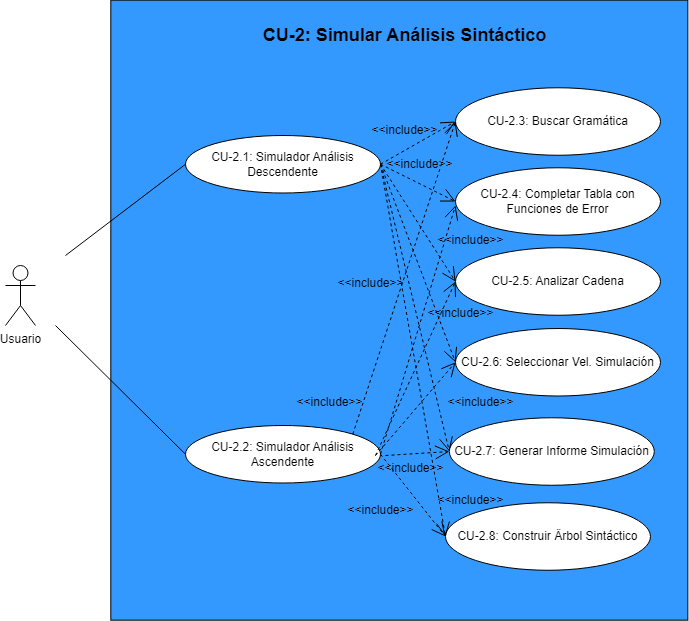
\includegraphics[scale=0.55]{figuras/Cap7/CU2.png}
 	\caption{CU-2 Simular análisis sintáctico predictivo}
 	\label{fig:CU2}
       \end{center}
   \end{figure}
  
 La especificación del caso de uso se muestra en la tabla \ref{tabla715}.

 \begin{longtable}[H]{|>{\columncolor[rgb]{0.63,0.79,0.95}}m{6cm} | m{8.5cm} |}
 \caption{Caso de uso: CU-2 Simular análisis sintáctico} \\
 \endfirsthead
 \multicolumn{2}{c}
 {{ \tablename\ \thetable{} -- continúa de la página anterior}} \\
 \endhead
 \hline \multicolumn{2}{|r|}{{Continúa en la página siguiente}} \\ \hline
 \endfoot
 \hline
 \endlastfoot
  \hline
  \textbf{Nombre} & \textbf{CU-2. Simular análisis sintáctico}. \newline \textbf{Nivel}: 1  \\ \hline
   \textbf{Descripción} & Permite al usuario realizar la simulación de un analizador sintáctico usando  una gramática.\\ \hline
  \textbf{Actores} & Usuario \\ \hline 
  \textbf{Casos de uso} & 
     \begin{enumerate}
     \item \textbf{CU-2.1. Simular Análisis Descendente Predictivo}: lleva a cabo el análisis sintáctico descendente predictivo de una gramática de contexto libre.
     \item \textbf{CU-2.2. Buscar gramática}: realiza la búsqueda en el sistema de una gramática de contexto libre guardada con anterioridad.
     \end{enumerate} \\ \hline
                                 
  \textbf{Flujo de eventos principal} & 
     \begin{enumerate}
     \item Se \textit{selecciona} la gramática que se desea simular.
     \item Se \textit{realiza} el análisis sintáctico descendente predictivo.
     \end{enumerate}\\ \hline
  \textbf{Flujo de eventos alternativo} & Si se produce un fallo durante el paso 1, se procede como sigue:
     \begin{enumerate}
     \item Se \textit{informa} al usuario que se ha podido cargar la gramática seleccionada.
     \item Se \textit{aborta} la selección de la gramática y no se podrá llevar a cabo la  simulación de dicha gramática.
     \item Se redirecciona a la pantalla de simulación.
     \end{enumerate}   
   \label{tabla715}
 \end{longtable}

 A continuación, se refinará cada uno de los casos de uso que componen el caso de uso CU-2.

 \subsubsection{CU-2.1. Simular Análisis Descendente Predictivo}

 Este caso de uso representa la simulación del análisis sintáctico descendente predictivo de una gramática de contexto libre. En la figura \ref{fig:CU21} se muestra la representación gráfica del caso de uso y en la  tabla \ref{tabla716} se muestra su representación tabular. Los sub-casos de uso que lo conforman son:

 \begin{itemize}
  \item \textbf{CU-2.1.1 Gestionar Tabla Predictiva}.
  \item \textbf{CU-2.1.2 Gestionar Conjunto Primero y Siguiente}.
 \end{itemize}

Este caso de uso CU-2.1 también interactúa con los siguientes casos de uso:
 \begin{itemize}
  \item \textbf{CU-2.2. Buscar Gramática}.
  \item \textbf{CU-2.3. Completar Tabla con Funciones de Error}.
  \item \textbf{CU-2.4. Analizar Cadena}.
  \item \textbf{CU-2.5. Seleccionar Velocidad Simulación}.
  \item \textbf{CU-2.6. Generar Informe Simulación}.
  \item \textbf{CU-2.7. Construir Árbol Sintáctico}.
 \end{itemize}


  \begin{figure}[H]
       \begin{center} 
 	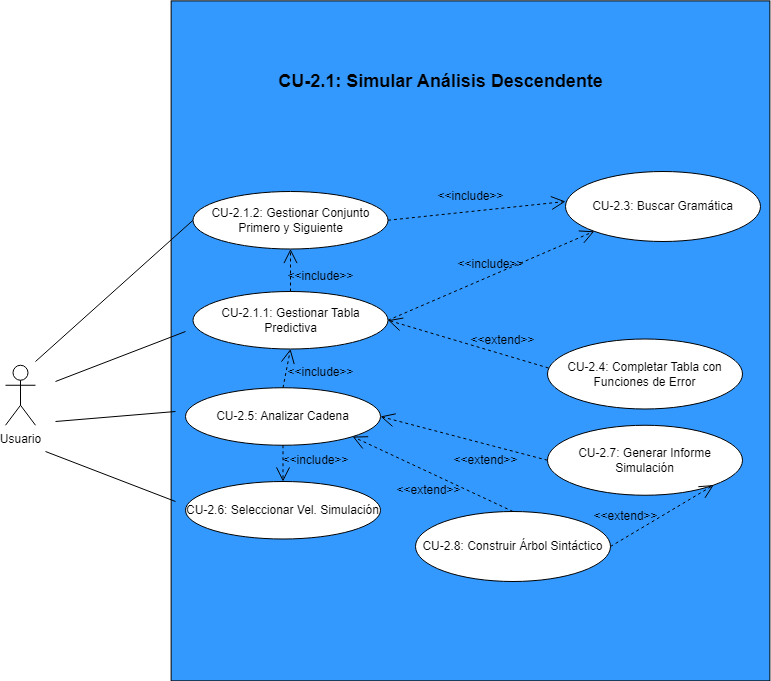
\includegraphics[scale=0.55]{figuras/Cap7/CU21.png}
 	\caption{CU-2.1 Simular Análisis descendente}
 	\label{fig:CU21}
       \end{center}
   \end{figure}
  
 \begin{longtable}[H]{|>{\columncolor[rgb]{0.63,0.79,0.95}}m{6cm} | m{8.5cm} |}
 \caption{Caso de uso: CU-2.1 Simular Análisis descendente predictivo} \\
 \endfirsthead
 \multicolumn{2}{c}
 {{ \tablename\ \thetable{} -- continúa de la página anterior}} \\
 \endhead
 \hline \multicolumn{2}{|r|}{{Continúa en la página siguiente}} \\ \hline
 \endfoot
 \hline
 \endlastfoot
  \hline
  \textbf{Nombre} & \textbf{CU-2.1. Simular Análisis descendente}. \newline \textbf{Nivel}: 2  \\ \hline
  \textbf{Descripción} & Permite al usuario realizar la simulación del análisis sintáctico descendente de una gramática de contexto libre.\\ \hline                 
  \textbf{Actores} & Usuario \\ \hline
  \textbf{Casos de uso} & 
     \begin{enumerate}
     \item \textbf{CU-2.1.1. Gestionar tabla predictiva}: \textit{gestionar} la tabla predictiva  necesaria para llevar a cabo la simulación.
     \item \textbf{CU-2.3. Buscar gramática}: realiza la búsqueda en el sistema de una gramática de contexto libre guardada con anterioridad.
     \item \textbf{CU-2.4. Completar tabla con funciones de error}: si el usuario lo desea, puede \textit{completar} la tabla predictiva con funciones para el tratamiento de los errores  que se 	puedan producir.
     \item \textbf{CU-2.1.2. Gestionar conjunto primero y siguiente}: \textit{gestionar} el  conjunto primero y siguiente de una gramática de contexto libre, necesarios para crear la tabla predictiva.			  
     \item \textbf{CU-2.5. Analizar cadena}: \textit{realiza} el análisis sintáctico descendente predictivo de una cadena.
     \item \textbf{CU-2.6. Seleccionar velocidad de simulación}: \textit{selecciona} la velocidad a la que se llevará a cabo la simulación: paso a paso o continua.
     \item \textbf{CU-2.7. Generar informe de la simulación}: una vez terminado el proceso de simulación, el usuario puede obtener un informe con todos los detalles.
     \item \textbf{CU-2.8. Construir Árbol Sintáctico}: se construirá el árbol sintáctico de la derivación correspondiente.
     \end{enumerate} \\ \hline
                                 
  \textbf{Flujo de eventos principal} & 
     \begin{enumerate}
     \item Se \textit{selecciona} la gramática que se desea simular.
     \item Se \textit{construye} el conjunto primero y siguiente.\item Se \textit{crea} la tabla predictiva con los datos de los pasos anteriores.
     \item Si se desea, se puede \textit{completar} la tabla predictiva con funciones de tratamiento de errores.
     \item Una vez que se tiene todo lo anterior, se procede a analizar una cadena con el simulador.
     \item Se \textit{elige} la velocidad de simulación: paso a paso o continua.
     \item Se \textit{escoge} si se desea construir de forma paralela a la derivación el árbol sintáctico.
     \item Se \textit{genera} el informe de la simulación que se ha llevado a cabo en los pasos anteriores.
     \end{enumerate}\\ \hline
                     
  \textbf{Flujo de eventos alternativo} & Si se produce un fallo durante el paso 1, se procede como sigue:
     \begin{enumerate}
     \item Se \textit{informa} al usuario que no se ha podido cargar la gramática seleccionada.
     \item Se \textit{aborta} la selección de la gramática y no se podrá llevar a cabo la  simulación.
     \item Se redirecciona a la pantalla de simulación.			\end{enumerate}    \\ \hline
  \textbf{Flujo de eventos alternativo} & Si se produce un fallo durante el paso 3, se procede como sigue:
     \begin{enumerate}
     \item Se \textit{informa} al usuario que se ha podido crear la tabla predictiva.
     \item Se \textit{aborta} la creación de la tabla predictiva y no se podrá llevar a cabo la simulación hasta que todos los datos sean correctos.
     \item Se redirecciona a la pantalla de simulación.
     \end{enumerate}   \\ \hline
  \textbf{Flujo de eventos alternativo} & Si se produce un fallo durante el paso 5, se procede como sigue:
     \begin{enumerate}
     \item Se \textit{informa} al usuario que no se ha podido analizar la cadena introducida.
     \item Se \textit{aborta} el análisis y no se podrá llevar a cabo hasta que todos los datos sean correctos.
     \item Se redirecciona a la pantalla de simulación.			\end{enumerate}   \\ \hline
 \textbf{Flujo de eventos alternativo} & Si se produce un fallo durante el paso 7, se procede como sigue:
     \begin{enumerate}
     \item Se \textit{informa} al usuario que no se ha podido generar el informe de la simulación.
     \item Se \textit{aborta} la generación del informe y no se podrá obtener el informe.
     \item Se redirecciona a la pantalla de simulación.			\end{enumerate}
   \label{tabla716}
 \end{longtable}

 El caso de uso \textit{CU-2.1.1} no se refinará más, puesto que se trata de un proceso simple, que puede ser fácilmente traducido a una implementación posterior sin necesidad de ser refinado.


\subsubsection{CU-2.1.2. Gestionar conjunto Primero y Siguiente}

Este caso de uso es un proceso simple que consiste en crear los conjuntos primero y siguiente de la gramática, necesarios para crear las tablas de análisis en el análisis sintáctico descendente predicitivo. Por tanto, este proceso no será refinado de forma más exhaustiva.

\subsubsection{CU-2.2. Buscar gramática}

Este caso de uso es un proceso simple que consiste en seleccionar una gramática de entre las que se encuentran cargadas en el simulador. Por tanto, este proceso no será refinado de forma más exhaustiva.


\subsubsection{CU-2.3. Completar tabla con funciones de error}

Este caso de uso es un proceso simple en el cual, una vez construida la tabla del análisis sintáctico, se completa con la funciones de error. Por tanto, este proceso no será refinado de forma más exhaustiva.

 \subsubsection{CU-2.4. Analizar cadena}

 Este caso de uso es un proceso simple en el que se lleva a cabo el análisis sintáctico descendente de una cadena. Por tanto, este proceso no será refinado de forma más exhaustiva.

 \subsubsection{CU-2.5. Selecciona velocidad de simulación}

 Este caso de uso es un proceso simple que consiste en seleccionar entre los dos tipos de velocidad de simulación: paso a paso o continuo. Por tanto, este proceso no será refinado de forma más exhaustiva.

 \subsubsection{CU-2.6. Generar informe de simulación}

 Este caso de uso es un proceso simple que consiste en generar un informe con todos los datos del análisis sintáctico creados durante la simulación, el cual podrá ver y descargar el usuario. Por tanto, este proceso no será refinado de forma más exhaustiva.

 \subsubsection{CU-2.7. Construir Árbol Sintáctico Descendente}

 Este caso de uso es un proceso simple que consiste en generar la construcción del árbol sintáctico descendente correspondiente a la derivación que se está realizando en dicho momento. Esta generación del árbol puede ser tanto instantánea como paso a paso y se hará de forma paralela a la propia derivación.


 \subsection{CU-3. Consultar Tutorial}

 Este caso de uso representa la consulta del tutorial de la aplicación. En la figura \ref{fig:CU3} se muestra la representación gráfica de este caso de uso, que está formada por los siguientes sub-casos de uso:

 \begin{itemize}
  \item \textbf{CU-3.1. Consultar una lección}.
  \item \textbf{CU-3.2. Obtener recurso del tutorial}.
  \item \textbf{CU-3.3. Navegar por el recurso seleccionado}.

 \end{itemize}

 En este caso de uso se muestran flechas que se dirige desde un caso de uso al usuario. Esto representa el hecho de que el usuario visualiza el tutorial por pantalla.

  \begin{figure}[H]
       \begin{center} 
 	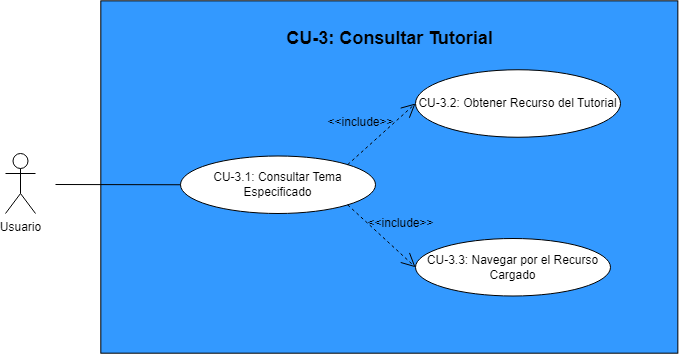
\includegraphics[scale=0.55]{figuras/Cap7/CU3.png}
 	\caption{CU-3: Consultar Tutorial}
 	\label{fig:CU3}
       \end{center}
   \end{figure}

 La especificación del caso de uso se muestra en la tabla \ref{tabla713}.


 \begin{longtable}[H]{|>{\columncolor[rgb]{0.63,0.79,0.95}}m{6cm} | m{8.5cm} |}
 \caption{Caso de uso: CU-3. Consultar Tutorial} \\

 \endfirsthead

 \multicolumn{2}{c}
 {{ \tablename\ \thetable{} -- continúa de la página anterior}} \\
 \endhead
 \hline \multicolumn{2}{|r|}{{Continúa en la página siguiente}} \\ \hline
 \endfoot
 \hline
 \endlastfoot
  \hline
  \textbf{Nombre} & \textbf{CU-3. Consultar Tutorial}.\newline \textbf{Nivel}: 1  \\ \hline
  \textbf{Descripción} & Permite al usuario consultar el tutorial de la aplicación.\\ \hline
  \textbf{Actores} & Usuario \\ \hline
  \textbf{Casos de uso} & 
     \begin{enumerate}
     \item \textbf{CU-3.1. Consultar una lección}: permite \textit{consultar} una lección del tutorial.
     \item \textbf{CU-3.2. Obtener recurso del tutorial}: permite \textit{obtener} una lección del tutorial. 
     \item \textbf{CU-3.3. Navegar por el recurso seleccionado}: permite \textit{navegar} por una lección del tutorial.
     \end{enumerate} \\ \hline
                                 
  \textbf{Flujo de eventos principal} & 
     \begin{enumerate}
     \item Se \textit{obtiene} un recurso del tutorial (especificado por el usuario).
     \item El usuario \textit{navega} por el recurso.
     \item El usuario \textit{accede} a otro recurso a través del enlace (para lo que se vuelve al paso 1), o sigue navegando por el mismo.
     \end{enumerate}\\ \hline
                     
  \textbf{Flujo de eventos alternativo} & Si se produce algún error al \textit{cargar} o \textit{navegar} por un recurso del tutorial, se informa al usuario y se restablece el recurso previo (cerrando el tutorial en caso de que se produzca un fallo).
   \label{tabla713}
 \end{longtable}

Nótese que lo que aquí se llama recurso del tutorial, es realmente una \textit{lección} del tutorial. El hecho de de\-no\-mi\-nar\-lo recurso implica que el fichero en cuestión (un recurso del simulador) es buscado y cargado, y, por tanto, contiene una lección del tutorial.

Este caso de uso no es necesario refinarlo exhaustivamente ya que es un proceso sencillo de traducir e implementar, por lo que se realizará sin mayores complicaciones.

 \subsection{CU-4. Consultar Ayuda}

 Este caso de uso representa la consulta de la ayuda de la aplicación. En la figura \ref{fig:CU4} se muestra la representación gráfica de este caso de uso, que está formada por los siguientes sub-casos de uso:

 \begin{itemize}
  \item \textbf{CU-4.1. Consultar un capítulo}.
  \item \textbf{CU-4.2. Obtener recurso de la ayuda}.
  \item \textbf{CU-4.3. Navegar por el recurso seleccionado}.
 \end{itemize}

 En este caso de uso se muestran flechas que se dirige desde un caso de uso al usuario. Esto representa el hecho de que el usuario visualiza la ayuda por pantalla.

 \begin{figure}[H]
       \begin{center} 
 	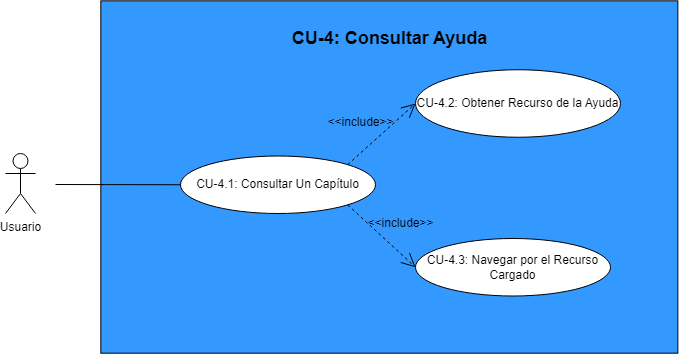
\includegraphics[scale=0.55]{figuras/Cap7/CU4.png}
 	\caption{CU-4: Consultar Ayuda}
 	\label{fig:CU4}
       \end{center}
   \end{figure}

 La especificación del caso de uso se muestra en la tabla \ref{tabla714}.

 \begin{longtable}[H]{|>{\columncolor[rgb]{0.63,0.79,0.95}}m{6cm} | m{8.5cm} |}
 \caption{Caso de uso: CU-4. Consultar Ayuda} \\
 \endfirsthead
 \multicolumn{2}{c}
 {{ \tablename\ \thetable{} -- continúa de la página anterior}} \\
 \endhead
 \hline \multicolumn{2}{|r|}{{Continúa en la página siguiente}} \\ \hline
 \endfoot
 \hline
 \endlastfoot
  \hline
  \textbf{Nombre} & \textbf{CU-4. Consulta de la ayuda}. \newline \textbf{Nivel}: 1  \\ \hline
  \textbf{Descripción} & Permite al usuario consultar la ayuda de la aplicación.\\ \hline
  \textbf{Actores} & Usuario \\ \hline
  \textbf{Casos de uso} & 
     \begin{enumerate}
     \item \textbf{CU-4.1. Consultar un capítulo}: permite \textit{consultar} un capítulo de la ayuda.
     \item \textbf{CU-4.2. Obtener recurso de la ayuda}: permite \textit{obtener} un capítulo de la ayuda.
     \item \textbf{CU-4.3. Navegar por el recurso seleccionado}: permite \textit{navegar} por un capítulo de la ayuda.
     \end{enumerate} \\ \hline
                                 
  \textbf{Flujo de eventos principal} & 
     \begin{enumerate}
     \item Se \textit{obtiene} un recurso de la ayuda (especificado por el usuario).
     \item El usuario \textit{navega} por el recurso.
     \item El usuario \textit{accede} a otro recurso a través del enlace (para lo que se vuelve al paso 1), o sigue navegando por el mismo.
     \end{enumerate}\\ \hline
                     
  \textbf{Flujo de eventos alternativo} & Si se produce algún error al \textit{cargar} o \textit{navegar} por un recurso de la ayuda, se informa al usuario y se restablece el recurso previo (cerrando la ayuda en caso de que se produzca un fallo).
   \label{tabla714}
 \end{longtable}

Nótese que lo que aquí se llama \textit{recurso} de la ayuda (al igual que sucedió con el tutorial), es realmente un \textit{capítulo} de la ayuda. El hecho de de nominarlo recurso implica que el fichero en cuestión (un recurso del simulador) es buscado y cargado, y por tanto, contiene un capítulo de la ayuda.

Al igual que en el caso de uso anterior, no es necesario un refinamiento más profundo, ya que es una tarea sencilla de implementar y que no supone una mayor complejidad.

 \section{Validación de los casos de uso }

Para asegurar que los casos de uso cumplen con los requisitos funcionales establecidos en el capítulo anterior, se llevará a cabo una validación exhaustiva. Esta validación garantizará que los casos de caso de uso se corresponden adecuadamente con los requisitos del sistema y funcionan de manera esperada en distintos escenarios.

% El proceso de validación consistirá en revisar cada caso de uso y verificar que todos los pasos y alternativas responden a los requisitos funcionales descritos. Se documentarán cualquier discrepancia o área de mejora, asegurando que el sistema final sea robusto y cumpla con las expectativas de los usuarios.

% Los resultados de la validación se presentarán en un informe detallado que incluirá tanto las conformidades como las no conformidades identificadas durante el proceso. Este informe servirá como guía para las futuras fases de desarrollo y refinamiento del sistema.

% De esta manera, se garantiza que el sistema no solo cumple con los requisitos establecidos, sino que también es eficiente y efectivo en su funcionamiento, proporcionando una experiencia satisfactoria para los usuarios.
%%%%%%%%%

 \subsection{Validación del Módulo de Edición de Gramática}

 La primera validación que se realizará será del módulo de edición respecto a los requisitos funcionales del sistema. El resultado de esta validación se recoge en la tabla \ref{val1}.

 \begin{table}[H]
 \begin{center}

  \caption{Matriz de correspondencia RF-Casos de uso}
 
 \resizebox{17cm}{!} {
 \begin{tabular}[c]{| c | c | c | c | c | c | c |c |c |c |c |c |c |c |c |}
 \hline

   \multicolumn{15}{|c|}{\textbf{Casos de uso}} \\ \hline
   \multirow{15}{0.3cm}{\begin{sideways}\textbf{Requisitos funcionales  \ \ \ \ \ \ \ \ \ \ \ \ \ \ \ }\end{sideways}} 
  
  & & CU-1.1 & CU-1.2 & CU-1.3 & CU-1.4 & CU-1.5 & CU-1.6 & CU-1.7 & CU-1.8 & CU-1.9 & CU-1.10 & CU-1.11 & CU-1.12 & CU-1.13\\ 
  \cline{2-15}
  &RF-E-1 & X &  & & & & & & & & & & &   \\ 
  \cline{2-15}
  &RF-E-2 & X & X & & & & & & & & & & &  \\ 
  \cline{2-15}
  &RF-E-3 &  &  & X& & & & & & & & & &  \\ 
  \cline{2-15}
  &RF-E-4 &  &  & X & & & & & & & & & &  \\ 
  \cline{2-15}
  &RF-E-5 &  &  & X & & & & & & & & & &  \\ 
  \cline{2-15}
   &RF-E-6 &  &  &  & X& & & & & & & & &  \\ 
  \cline{2-15}
   &RF-E-7 &  &  & & & & &X & & & & & &  \\ 
  \cline{2-15}
   &RF-E-8 &  &  & & & & & & & & & &X &  \\ 
  \cline{2-15}
   &RF-E-9 &  &  & & & & & & & X& & & &  \\ 
  \cline{2-15}
   &RF-E-10 &  &  & & & X& & & & & & & &  \\ 
  \cline{2-15}
   &RF-E-11 &  &  & & & & & X& & & & & &  \\ 
  \cline{2-15}
   &RF-E-12 &  &  & & & & X& & & & &X & & \\ 
  \cline{2-15}
   &RF-E-13 &  &  & & & & & & X& & & & & \\ 
  \cline{2-15}
   &RF-E-14 &  & & & & & & &X & & & & & X \\ 
  \cline{2-15}
   &RF-E-15 &  &  & & & & & & & &X & & &  \\ \hline

 \end{tabular}
 }
  \label{val1}
  \end{center}
 \end{table}

\newpage

 \subsection{Validación del Módulo de Simulación de Gramática}

 La segunda validación que se realizará será del módulo de simulación respecto a los requisitos funcionales del sistema. El resultado de esta validación se recoge en la tabla \ref{val2}.

 \begin{table}[H]
 \begin{center}

  \caption{Matriz de correspondencia RF-Casos de uso}
 
 %\resizebox{17cm}{!} { QUITADO
 \begin{tabular}[c]{| c | c | c | c | c | c | c |c |c |}
 \hline

   \multicolumn{9}{|c|}{\textbf{Casos de uso}} \\ \hline
   \multirow{10}{0.3cm}{\begin{sideways}\textbf{Requisitos funcionales  \ \ \ \ \ \ \ \ \ \ \ \ \ \ \ }\end{sideways}} 
  
  & & CU-2.1 & CU-2.2 & CU-2.3 & CU-2.4 & CU-2.5 & CU-2.6 & CU-2.7 \\ 
  \cline{2-9}
  &RF-S-1 & X & X & & & & &    \\ 
  \cline{2-9}
  &RF-S-2 & X & X & & & & &    \\ 
  \cline{2-9}
  &RF-S-3 &  &  & &X & & &     \\ 
  \cline{2-9}
  &RF-S-4 &  &  & &X & & &    \\ 
  \cline{2-9}
  &RF-S-5 &  &  & & X& & &     \\ 
  \cline{2-9}
   &RF-S-6 &  &  & &X & & &    \\ 
  \cline{2-9}
   &RF-S-7  &  &  & & & X& &    \\ 
  \cline{2-9}
   &RF-S-8  &  &  & & &X & &    \\ 
  \cline{2-9}
   &RF-S-9 &  &  & & & &X &    \\ 
  \cline{2-9}
   &RF-S-10 &  &  & & & &X &    \\ 
  \cline{2-9}
   &RF-S-11 &  &  & & & &X &     \\ 
  \cline{2-9}
   &RF-S-12 &  &  & & & & &X   \\ 
  \cline{2-9}
   &RF-S-13 &  &  & &X & & &    \\ 
  \cline{2-9}
   &RF-S-14 &  &  & & & & &X    \\ 
  \cline{2-9}
   &RF-S-15 &  &  & & & & & X   \\
   \cline{2-9}
   &RF-S-16 &  &  & X& & & &X    \\ 
   \cline{2-9}
   &RF-S-17 &  &  & & & & &X    \\ 
  \cline{2-9}
   &RF-S-18 &  &  & & & & & X   \\ \hline
 \end{tabular}
 %} QUUITADO
  \label{val2}
  \end{center}
 \end{table}


 \subsection{Validación del Módulo del Tutorial}

 La matriz de validación de este Módulo se recoge en la tabla \ref{val3}.

 \begin{table}[H]
 \begin{center}

  \caption{Matriz de correspondencia RF-CU, Módulo tutorial}
 
 %\resizebox{7cm}{!} {
 \begin{tabular}[c]{| c | c | c | c | c | }
 \hline

   \multicolumn{5}{|c|}{\textbf{Casos de uso}} \\ \hline
   \multirow{4}{0.3cm}{\begin{sideways}\textbf{R. funcionales}\end{sideways}} 
  
  & & CU-3.1 & CU-3.2 & CU-3.3 \\ 
  \cline{2-5}
  &RF-T-1 & X &  &   \\ 
  \cline{2-5}
  &RF-T-2 &  & X & X  \\
  \cline{2-5}
  &RF-T-3 &  & X &   \\    \hline

 \end{tabular}
 %}
  \label{val3}
  \end{center}
 \end{table}

 \subsection{Validación del Módulo de la Ayuda}

 La matriz de validación de este Módulo se recoge en la tabla \ref{val4}.

 \begin{table}[H]
 \begin{center}

  \caption{Matriz de correspondencia RF-CU, Módulo ayuda}
 
 %\resizebox{7cm}{!} {
 \begin{tabular}[c]{| c | c | c | c | c | }
 \hline

   \multicolumn{5}{|c|}{\textbf{Casos de uso}} \\ \hline
   \multirow{5}{0.3cm}{\begin{sideways}\textbf{R.  funcionales}\end{sideways}} 
  
  & & CU-4.1 & CU-4.2 & CU-4.3 \\ 
  \cline{2-5}
  &RF-A-1 & X &  &   \\ 
  \cline{2-5}
  &RF-A-2 &  & X & X  \\
  \cline{2-5}
  &RF-A-3 &  & X &   \\\hline

 \end{tabular}
 %}
  \label{val4}
  \end{center}
 \end{table}

\part{Diseño}
\chapter{Diseño de paquetes} \label{cap:diseño-paquetes}


\section{Introducción}


% Este capítulo muestra cómo se agrupan por cercanía funcional y semántica las clases y demás elementos del sistema en diferentes paquetes, que permiten su manipulación en grupos. Se identificarán los paquetes más
% relevantes del sistema y se describirá su finalidad.

 \section{Especificación de los paquetes de la aplicación}

% Los paquetes en los que se puede descomponer el simulador se obtienen a partir de los subsistemas que lo constituyen:
% \begin{itemize}
%  \item \textbf{Paquete es.uco.simAS}.
%  \item \textbf{Paquete editor}.
%  \item \textbf{Paquete simulador}.
%  \item \textbf{Paquete util.gramatica}.
%  \item \textbf{Paquete centroayuda}.
%  \item \textbf{Paquete resources}.
% \end{itemize}

% \subsection{Paquete es.uco.simAS}

% Este es el paquete general de la aplicación y contiene a los demás paquetes. Al ser un proyecto de la \textit{Universidad de Córdoba}, se ha seguido la recomendaciones de Java a la hora de nombrar los paquetes y se ha supuesto el dominio \textbf{es.uco.simAS} para nombrar este paquete.

% \subsection{Paquete editor}

% El paquete \textbf{editor} contiene todas las clases del editor de gramáticas (tanto las de información como las que solamente contienen elementos gráficos). El paquete importa a los paquetes \textit{util.gramatica}, para hacer uso de las gramáticas de contexto libre; \textit{centroayuda}, para interactuar con la ayuda; \textit{resources}, donde se almacenan todos los iconos y recursos gráficos para la interfaz; y el \textit{paquete del simulador}, lo importa para poder transferirle una gramática (Figura  \ref{paqeditor}).

% \begin{figure}[H]
%       \begin{center} 
% 	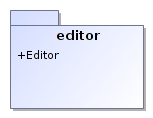
\includegraphics[scale=0.6]{figuras/Cap8/paqeditor.jpg}
% 	\caption{Paquete editor}
% 	\label{paqeditor}
%       \end{center}
%   \end{figure}


% \subsection{Paquete simulador}

% El paquete \textbf{simulador} contiene todas las clases del simulador de gramáticas (tanto las de información como las que solamente contienen elementos gráficos). El paquete importa a los paquetes \textit{util.gramatica}, para hacer uso de las gramáticas de contexto
% libre; \textit{centroayuda}, para interactuar con la ayuda; \textit{resources}, donde se almacenan todos los iconos y recursos gráficos para la interfaz; y el \textit{paquete del editor} lo  importa para poder transferirle una gramática de vuelta (Figura  \ref{paqsimulador}).

% \begin{figure}[H]
%       \begin{center} 
% 	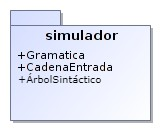
\includegraphics[scale=0.6]{figuras/Cap8/paqsimulador.jpg}
% 	\caption{Paquete simulador}
% 	\label{paqsimulador}
%       \end{center}
%   \end{figure}

% \subsection{Paquete util.gramatica}

% Este paquete contiene todas las clases relacionadas con las gramáticas de contexto libre, además de la clase que representa a las funciones de error (Figura \ref{paqgramatica}).

% \begin{figure}[H]
%       \begin{center} 
% 	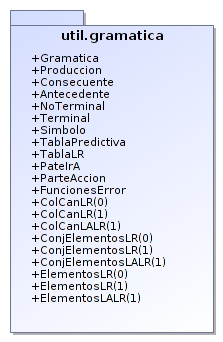
\includegraphics[scale=0.6]{figuras/Cap8/paqgramatica.jpg}
% 	\caption{Paquete util.gramatica}
% 	\label{paqgramatica}
%       \end{center}
%   \end{figure}

% \subsection{Paquete centroayuda}

% Este paquete contiene la ventana del centro de ayuda y todos los recursos de la ayuda de SimAS (todos los capítulos en formato html de la ayuda) (Figura \ref{paqayuda}=.

% \begin{figure}[H]
%       \begin{center} 
% 	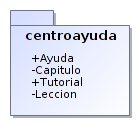
\includegraphics[scale=0.6]{figuras/Cap8/paqayuda.jpg}
% 	\caption{Paquete centroayuda}
% 	\label{paqayuda}
%       \end{center}
%   \end{figure}

% \subsection{Paquete resources}

% Este paquete contiene todos los recursos gráficos utilizados por los componentes de la interfaz gráfica de SimAS (iconos, imágenes, tipos de letra, etcétera). Nótese que los componentes de la ayuda se han situado en el paquete \textit{centroayuda} en lugar de hacerlo en este. Así se asegura que todos los recursos gráficos usados por el programa están en el mismo paquete y separados de otros recursos que sólo usa un módulo concreto, como es el Centro de ayuda.

% Este paquete aparece vacío en el diagrama porque realmente no contiene
% ninguna clase de las especificadas en el estudio del sistema, sino que contiene recursos gráficos de la interfaz (que son demasiados como para enumerarlos en el diagrama).

 \section{Diagrama de paquetes de la aplicación}

% En la figura \ref{dpaquetes} se muestra el diagrama de paquetes del simulador, según lo analizado anteriormente. Nótese que en los paquetes únicamente se muestran los elementos de información finales de la aplicación (las clases que representan objetos de la interfaz no se recogen en este diagrama, puesto que complicarían en gran medida
% su presentación y comprensión). 

%  \begin{figure}[H]
%       \begin{center} 
% 	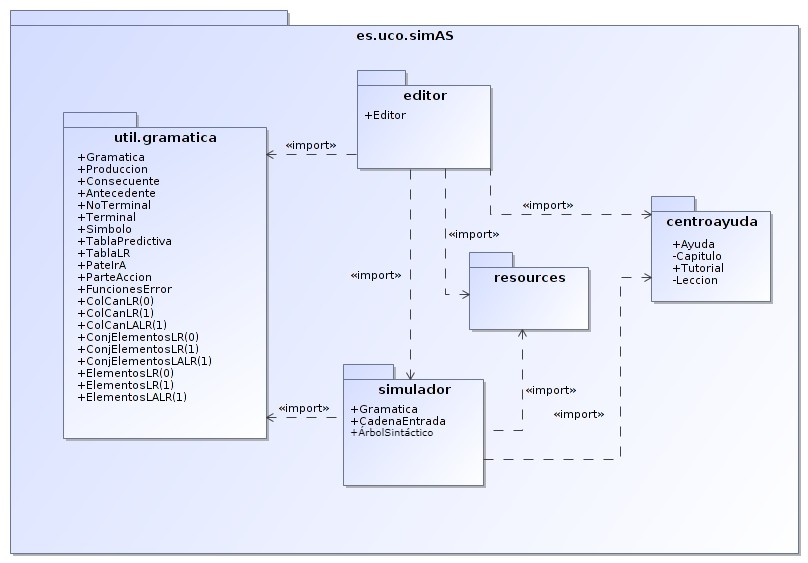
\includegraphics[scale=0.55]{figuras/Cap8/paquetes.jpg}
% 	\caption{Diagrama de paquetes}
% 	\label{dpaquetes}
%       \end{center}
%   \end{figure}



\chapter{Diseño de clases} \label{cap:diseño_clases}

\section{Introducción}

En este capítulo se realizará una breve introducción sobre el diagrama de clases y posteriormente, un análisis de las clases que participan en el modelo de información del simulador SimAS 3.0. Para ello, se especificarán los atributos, métodos y las relaciones existentes entre las mismas, terminándose con un diagrama de clases general de todo el sistema.

El propósito de un diagrama de clases es el de representar los objetos fundamentales del sistema, es decir, los que percibe el usuario y con los que espera tratar para completar su tarea. Una clase define el ámbito de definición de un conjunto de objetos.

Cada clase se representa en un rectángulo con tres apartados:
\begin{itemize}
\item Nombre de la clase.
\item Atributos de la clase.
\item Operaciones de la clase.
\end{itemize}

En SimAS 3.0, el diseño de clases sigue el patrón Model-View-Controller (MVC), donde las clases del modelo representan la lógica de negocio y los datos de las gramáticas de contexto libre, mientras que las clases de la vista y controlador manejan la interfaz de usuario y la interacción con el usuario.


\section{Diseño de clases por paquetes}

El sistema SimAS 3.0 está organizado en 8 paquetes principales que contienen un total de 51 clases Java. Para una mejor comprensión y organización, este capítulo presenta las clases agrupadas por paquetes, siguiendo la arquitectura por capas definida en el Capítulo 8.

Cada sección dedicada a un paquete incluye:
\begin{itemize}
    \item \textbf{Introducción}: propósito y responsabilidad del paquete.
    \item \textbf{Clases principales}: análisis detallado de cada clase con atributos y métodos.
    \item \textbf{Dependencias internas}: relaciones entre clases dentro del paquete.
    \item \textbf{Patrones de diseño}: patrones utilizados en el paquete.
\end{itemize}

\subsection{Paquete bienvenida}

El paquete \textbf{bienvenida} contiene las clases responsables de la inicialización y navegación principal de la aplicación SimAS 3.0. Este paquete implementa el patrón Singleton y Facade para gestionar el ciclo de vida de la aplicación.

\subsubsection{Clases del paquete bienvenida}

Este paquete contiene 2 clases principales que gestionan el punto de entrada y la navegación inicial del sistema.

\subsubsection{Clase Bienvenida}

Esta clase representa la pantalla de bienvenida de la aplicación SimAS 3.0, heredando de Application para ser el punto de entrada principal.

\begin{longtable}[H]{|>{\columncolor[rgb]{0.63,0.79,0.95}}m{6cm} | m{8.5cm} |}
 \caption{Clase Bienvenida}

\endfirsthead

\multicolumn{2}{c}
{{\tablename\ \thetable{} -- continúa de la página anterior}} \\
\endhead

\hline \multicolumn{2}{|r|}{{Continúa en la página siguiente}} \\ \hline
\endfoot

\hline
\endlastfoot

\hline
 \textbf{Nombre} & \textbf{Bienvenida}  \\ \hline
 
 \textbf{Descripción} & Representa la pantalla de bienvenida de la aplicación.  \\ \hline
                       
 \textbf{Atributos} & \begin{enumerate}
 		\item \textbf{stage}: Stage principal de la aplicación JavaFX.
 		\item \textbf{scene}: Scene que contiene la interfaz de bienvenida.
 		\item \textbf{root}: VBox principal que organiza el layout vertical.
 		\item \textbf{logo}: ImageView que muestra el logo de la aplicación.
 		\item \textbf{titulo}: Label con el título principal de SimAS 3.0.
 		\item \textbf{subtitulo}: Label con información adicional.
 		\item \textbf{selectorIdioma}: ComboBox para selección de idioma.
 		\item \textbf{botonContinuar}: Button para acceder al menú principal.
 		\item \textbf{bundle}: ResourceBundle para internacionalización.
 		\item \textbf{idiomaSeleccionado}: String con el código del idioma actual.
 		\item \textbf{preferencias}: Properties para guardar configuración.
 		\item \textbf{animacionFadeIn}: FadeTransition para animación de entrada.
 		\item \textbf{timeline}: Timeline para animaciones secuenciales.
 		\item \textbf{esPrimeraEjecucion}: boolean que indica si es la primera vez.
 		\item \textbf{versionAplicacion}: String con la versión actual.
 		\item \textbf{fechaCompilacion}: String con la fecha de compilación.
\end{enumerate} \\ \hline
 
\textbf{Métodos} & \begin{enumerate}
 		\item \textbf{start(Stage)}: método principal que inicializa la aplicación y configura la escena inicial.
 		\item \textbf{main(String[])}: punto de entrada estático de la aplicación JavaFX.
 		\item \textbf{inicializarInterfaz()}: configura todos los elementos visuales de la pantalla de bienvenida.
 		\item \textbf{configurarIdioma()}: detecta y configura el idioma por defecto del sistema.
 		\item \textbf{cargarRecursos()}: carga imágenes, estilos y recursos necesarios.
 		\item \textbf{crearLayoutPrincipal()}: crea el layout principal con VBox y elementos centrados.
 		\item \textbf{agregarLogo()}: añade el logo de la aplicación al centro.
 		\item \textbf{agregarTitulo()}: añade el título principal de la aplicación.
 		\item \textbf{agregarSelectorIdioma()}: crea el ComboBox para selección de idioma.
 		\item \textbf{agregarBotonContinuar()}: añade el botón para continuar al menú principal.
 		\item \textbf{configurarEstilos()}: aplica estilos CSS a todos los componentes.
 		\item \textbf{animarEntrada()}: ejecuta animaciones de entrada suaves.
 		\item \textbf{transitarAMenuPrincipal()}: realiza la transición suave al menú principal.
 		\item \textbf{guardarPreferenciasIdioma()}: guarda la selección de idioma del usuario.
 		\item \textbf{cargarPreferencias()}: carga preferencias guardadas anteriormente.
\end{enumerate} \\ \hline

\textbf{Métodos} & \begin{enumerate}
 		\item \textbf{verificarPrimeraEjecucion()}: determina si es la primera vez que se ejecuta.
 		\item \textbf{mostrarTutorialInicial()}: muestra tutorial básico para nuevos usuarios.
 		\item \textbf{centrarVentana()}: centra la ventana en la pantalla.
 		\item \textbf{establecerTamanoMinimo()}: establece el tamaño mínimo de la ventana.
 		\item \textbf{configurarEventosTeclado()}: configura atajos de teclado.
 		\item \textbf{limpiarRecursos()}: libera recursos antes de la transición.
\end{enumerate}                                 

 \label{tabla99}

\end{longtable}

\subsubsection{Clase MenuPrincipal}

La clase \textbf{MenuPrincipal} gestiona la interfaz principal de navegación de la aplicación SimAS 3.0, proporcionando acceso a todas las funcionalidades principales del sistema.

\begin{longtable}[H]{|>{\columncolor[rgb]{0.63,0.79,0.95}}m{6cm} | m{8.5cm} |}
\caption{Clase MenuPrincipal - Interfaz principal de navegación}
\endfirsthead
\multicolumn{2}{c}{{\tablename\ \thetable{} -- continúa de la página anterior}} \\
\endhead
\hline \multicolumn{2}{|r|}{{Continúa en la página siguiente}} \\ \hline
\endfoot
\hline
\endlastfoot
\hline
\textbf{Nombre} & \textbf{MenuPrincipal} \\ \hline
\textbf{Descripción} & Gestiona el menú principal de navegación (extends Application) \\ \hline
\textbf{Atributos} &
\begin{enumerate}
    \item \textbf{stage}: escena principal de la aplicación JavaFX.
    \item \textbf{scene}: escena que contiene la interfaz del menú.
    \item \textbf{root}: BorderPane que organiza el layout principal.
    \item \textbf{menuBar}: MenuBar con las opciones principales.
    \item \textbf{toolBar}: ToolBar con accesos rápidos.
    \item \textbf{contentArea}: área central para contenido dinámico.
    \item \textbf{statusBar}: barra de estado inferior.
    \item \textbf{bundle}: ResourceBundle para internacionalización.
    \item \textbf{currentModule}: módulo actualmente activo.
\end{enumerate} \\ \hline
\textbf{Métodos} &
\begin{enumerate}
    \item \textbf{start(Stage)}: método principal que inicializa la interfaz del menú.
    \item \textbf{main(String[])}: punto de entrada alternativo de la aplicación.
    \item \textbf{inicializarMenuBar()}: configura la barra de menú principal.
    \item \textbf{inicializarToolBar()}: configura la barra de herramientas.
    \item \textbf{inicializarStatusBar()}: configura la barra de estado.
    \item \textbf{abrirEditor()}: abre la ventana del editor de gramáticas.
    \item \textbf{abrirSimulador()}: abre la ventana del simulador.
    \item \textbf{abrirAyuda()}: abre el sistema de ayuda integrado.
    \item \textbf{abrirAcercaDe()}: muestra la ventana "Acerca de".
    \item \textbf{cambiarIdioma(String)}: cambia el idioma de la aplicación.
    \item \textbf{mostrarPreferencias()}: muestra el diálogo de preferencias.
    \item \textbf{salirAplicacion()}: cierra la aplicación correctamente.
    \item \textbf{actualizarTextos()}: actualiza todos los textos de la interfaz.
    \item \textbf{guardarEstado()}: guarda el estado actual de la aplicación.
    \item \textbf{cargarEstado()}: carga el estado guardado previamente.
    \item \textbf{mostrarMensajeEstado(String)}: muestra mensajes en la barra de estado.
    \item \textbf{configurarAtajosTeclado()}: configura los atajos de teclado globales.
\end{enumerate} \\ \hline
\textbf{Métodos} &
\begin{enumerate}
    \item \textbf{maximizarVentana()}: maximiza la ventana principal.
    \item \textbf{minimizarVentana()}: minimiza la ventana principal.
    \item \textbf{restaurarVentana()}: restaura el tamaño normal de la ventana.
    \item \textbf{centrarVentana()}: centra la ventana en la pantalla.
\end{enumerate}
\label{tabla_menu_principal}
\end{longtable}

\subsubsection{Dependencias internas del paquete bienvenida}

\begin{itemize}
    \item \textbf{Bienvenida $\rightarrow$ MenuPrincipal}: la clase Bienvenida crea y transita hacia MenuPrincipal después de la inicialización.
    \item \textbf{MenuPrincipal $\rightarrow$ Sistema}: MenuPrincipal coordina el acceso a todos los módulos principales (editor, simulador, ayuda).
\end{itemize}

\subsubsection{Patrones de diseño en el paquete bienvenida}

\begin{itemize}
    \item \textbf{Singleton}: implementado en Bienvenida para garantizar una única instancia de pantalla de bienvenida \cite{gamma1995design}.
    \item \textbf{Facade}: MenuPrincipal actúa como fachada simplificando el acceso a los módulos complejos del sistema \cite{gamma1995design}.
\end{itemize}

\subsection{Paquete gramática}

El paquete \textbf{gramática} contiene las clases fundamentales que representan el modelo de datos del simulador SimAS 3.0. Este paquete implementa el patrón de diseño Modelo-Vista-Controlador (MVC) donde las clases del modelo encapsulan toda la lógica de negocio relacionada con las gramáticas de contexto libre, incluyendo su definición, manipulación y análisis sintáctico.

Las clases de este paquete permiten:
\begin{itemize}
    \item Definir y manipular símbolos terminales y no terminales
    \item Crear y gestionar producciones gramaticales
    \item Construir y consultar tablas predictivas para análisis sintáctico
    \item Gestionar funciones de error para recuperación de errores
    \item Integración completa con la interfaz JavaFX mediante propiedades observables
\end{itemize}

\subsubsection{Clases del paquete gramática}

Este paquete contiene 11 clases principales que conforman el núcleo del modelo de datos de SimAS 3.0, organizadas jerárquicamente desde los elementos básicos hasta las estructuras complejas de análisis. Las clases se presentan en orden lógico de dependencia, desde las más básicas hasta las más complejas.

\subsubsection{Clase Simbolo}

La clase \textbf{Simbolo} es la clase base abstracta que representa cualquier símbolo en una gramática de contexto libre, sirviendo como superclase para Terminal y NoTerminal.

\begin{longtable}[H]{|>{\columncolor[rgb]{0.63,0.79,0.95}}m{6cm} | m{8.5cm} |}
\caption{Clase Simbolo - Clase base para símbolos gramaticales}
\endfirsthead
\multicolumn{2}{c}{{\tablename\ \thetable{} -- continúa de la página anterior}} \\
\endhead
\hline \multicolumn{2}{|r|}{{Continúa en la página siguiente}} \\ \hline
\endfoot
\hline
\endlastfoot
\hline
\textbf{Nombre} & \textbf{Simbolo} \\ \hline
\textbf{Descripción} & Clase base abstracta que representa un símbolo genérico en la gramática, proporcionando la estructura común para terminales y no terminales. \\ \hline
\textbf{Atributos} &
\begin{enumerate}
    \item \textbf{nombre}: StringProperty que contiene el nombre/valor del símbolo.
    \item \textbf{valor}: StringProperty que contiene información adicional del símbolo.
\end{enumerate} \\ \hline
\textbf{Métodos} &
\begin{enumerate}
    \item \textbf{Simbolo(String, String)}: constructor que inicializa nombre y valor.
    \item \textbf{getNombre()}: obtiene el nombre del símbolo.
    \item \textbf{setNombre(String)}: establece el nombre del símbolo.
    \item \textbf{nombreProperty()}: devuelve la propiedad observable del nombre.
    \item \textbf{getValor()}: obtiene el valor del símbolo.
    \item \textbf{setValor(String)}: establece el valor del símbolo.
    \item \textbf{valorProperty()}: devuelve la propiedad observable del valor.
\end{enumerate}
\label{tabla_simbolo}
\end{longtable}

\subsubsection{Clase Terminal}

La clase \textbf{Terminal} representa un símbolo terminal en la gramática, heredando de la clase Simbolo.

\begin{longtable}[H]{|>{\columncolor[rgb]{0.63,0.79,0.95}}m{6cm} | m{8.5cm} |}
\caption{Clase Terminal - Símbolos terminales de la gramática}
\endfirsthead
\multicolumn{2}{c}{{\tablename\ \thetable{} -- continúa de la página anterior}} \\
\endhead
\hline \multicolumn{2}{|r|}{{Continúa en la página siguiente}} \\ \hline
\endfoot
\hline
\endlastfoot
\hline
\textbf{Nombre} & \textbf{Terminal} \\ \hline
\textbf{Descripción} & Representa un símbolo terminal de la gramática, que son los símbolos básicos que no pueden ser reemplazados por otros símbolos. \\ \hline
\textbf{Atributos} & Hereda todos los atributos de Simbolo (nombre, valor). \\ \hline
\textbf{Métodos} &
\begin{enumerate}
    \item \textbf{Terminal(String, String)}: constructor que inicializa el terminal con nombre y valor.
    \item \textbf{toString()}: devuelve el nombre del terminal para representación textual.
\end{enumerate}
\label{tabla_terminal}
\end{longtable}

\subsubsection{Clase NoTerminal}

La clase \textbf{NoTerminal} representa un símbolo no terminal en la gramática, heredando de Simbolo y añadiendo funcionalidades específicas para el análisis sintáctico.

\begin{longtable}[H]{|>{\columncolor[rgb]{0.63,0.79,0.95}}m{6cm} | m{8.5cm} |}
\caption{Clase NoTerminal - Símbolos no terminales de la gramática}
\endfirsthead
\multicolumn{2}{c}{{\tablename\ \thetable{} -- continúa de la página anterior}} \\
\endhead
\hline \multicolumn{2}{|r|}{{Continúa en la página siguiente}} \\ \hline
\endfoot
\hline
\endlastfoot
\hline
\textbf{Nombre} & \textbf{NoTerminal} \\ \hline
\textbf{Descripción} & Representa un símbolo no terminal de la gramática, que puede ser reemplazado por secuencias de otros símbolos durante el análisis sintáctico. \\ \hline
\textbf{Atributos} &
\begin{enumerate}
    \item \textbf{simboloInicial}: boolean que indica si este no terminal es el símbolo inicial de la gramática.
    \item \textbf{primeros}: ObservableList de Terminal que contiene el conjunto primeros del no terminal.
    \item \textbf{siguientes}: ObservableList de Terminal que contiene el conjunto siguientes del no terminal.
\end{enumerate} \\ \hline
\textbf{Métodos} &
\begin{enumerate}
    \item \textbf{NoTerminal(String, String)}: constructor que inicializa el no terminal.
    \item \textbf{setSimboloInicial(boolean)}: marca este no terminal como símbolo inicial.
    \item \textbf{getSimboloInicial()}: verifica si es el símbolo inicial.
    \item \textbf{getPrimeros()}: obtiene el conjunto primeros.
    \item \textbf{setPrimeros( ObservableList<Terminal>)}: establece el conjunto primeros.
    \item \textbf{getSiguientes()}: obtiene el conjunto siguientes.
    \item \textbf{setSiguientes( ObservableList<Terminal>)}: establece el conjunto siguientes.
    \item \textbf{toString()}: devuelve el nombre del no terminal.
\end{enumerate}
\label{tabla_no_terminal}
\end{longtable}

\subsubsection{Clase Consecuente}

La clase \textbf{Consecuente} representa la parte derecha de una producción gramatical, conteniendo la secuencia de símbolos que reemplaza al antecedente.

\begin{longtable}[H]{|>{\columncolor[rgb]{0.63,0.79,0.95}}m{6cm} | m{8.5cm} |}
\caption{Clase Consecuente - Parte derecha de las producciones}
\endfirsthead
\multicolumn{2}{c}{{\tablename\ \thetable{} -- continúa de la página anterior}} \\
\endhead
\hline \multicolumn{2}{|r|}{{Continúa en la página siguiente}} \\ \hline
\endfoot
\hline
\endlastfoot
\hline
\textbf{Nombre} & \textbf{Consecuente} \\ \hline
\textbf{Descripción} & Representa el consecuente (lado derecho) de una producción gramatical, compuesto por una secuencia ordenada de símbolos. \\ \hline
\textbf{Atributos} &
\begin{enumerate}
    \item \textbf{conjSimbolos}: ObservableList de Simbolo que contiene la secuencia de símbolos del consecuente.
\end{enumerate} \\ \hline
\textbf{Métodos} &
\begin{enumerate}
    \item \textbf{Consecuente()}: constructor sin parámetros que inicializa la lista vacía.
    \item \textbf{getConjSimbolos()}: obtiene la lista de símbolos del consecuente.
    \item \textbf{setConjSimbolos(ObservableList <Simbolo>)}: establece la lista de símbolos del consecuente.
\end{enumerate}
\label{tabla_consecuente}
\end{longtable}

\subsubsection{Clase Antecedente}

La clase \textbf{Antecedente} representa la parte izquierda de una producción gramatical, conteniendo el símbolo no terminal que será reemplazado.

\begin{longtable}[H]{|>{\columncolor[rgb]{0.63,0.79,0.95}}m{6cm} | m{8.5cm} |}
\caption{Clase Antecedente - Parte izquierda de las producciones}
\endfirsthead
\multicolumn{2}{c}{{\tablename\ \thetable{} -- continúa de la página anterior}} \\
\endhead
\hline \multicolumn{2}{|r|}{{Continúa en la página siguiente}} \\ \hline
\endfoot
\hline
\endlastfoot
\hline
\textbf{Nombre} & \textbf{Antecedente} \\ \hline
\textbf{Descripción} & Representa el antecedente (lado izquierdo) de una producción gramatical, compuesto por un único símbolo no terminal. \\ \hline
\textbf{Atributos} &
\begin{enumerate}
    \item \textbf{simboloNT}: NoTerminal que representa el símbolo no terminal del antecedente.
\end{enumerate} \\ \hline
\textbf{Métodos} &
\begin{enumerate}
    \item \textbf{Antecedente()}: constructor sin parámetros que inicializa con valores vacíos.
    \item \textbf{Antecedente(NoTerminal)}: constructor con símbolo no terminal específico.
    \item \textbf{getSimboloNT()}: obtiene el símbolo no terminal del antecedente.
    \item \textbf{setSimboloNT(NoTerminal)}: establece el símbolo no terminal del antecedente.
    \item \textbf{toString()}: devuelve la representación textual del antecedente.
\end{enumerate}
\label{tabla_antecedente}
\end{longtable}

\subsubsection{Clase Produccion}

La clase \textbf{Produccion} representa una regla completa de producción en la gramática, compuesta por un antecedente y un consecuente.

\begin{longtable}[H]{|>{\columncolor[rgb]{0.63,0.79,0.95}}m{6cm} | m{8.5cm} |}
\caption{Clase Produccion - Reglas de producción gramatical}
\endfirsthead
\multicolumn{2}{c}{{\tablename\ \thetable{} -- continúa de la página anterior}} \\
\endhead
\hline \multicolumn{2}{|r|}{{Continúa en la página siguiente}} \\ \hline
\endfoot
\hline
\endlastfoot
\hline
\textbf{Nombre} & \textbf{Produccion} \\ \hline
\textbf{Descripción} & Representa una producción completa de la gramática, formada por un antecedente y un consecuente (secuencia de símbolos). \\ \hline
\textbf{Atributos} &
\begin{enumerate}
    \item \textbf{antec}: Antecedente que contiene el símbolo no terminal de la izquierda.
    \item \textbf{consec}: ObservableList de Simbolo que contiene la secuencia de símbolos del lado derecho.
    \item \textbf{numero}: int que identifica el número de la producción en la gramática.
\end{enumerate} \\ \hline
\textbf{Métodos} &
\begin{enumerate}
    \item \textbf{Produccion()}: constructor sin parámetros con inicialización básica.
    \item \textbf{Produccion(Antecedente, ObservableList<Simbolo>)}: constructor completo.
    \item \textbf{getAntec()}: obtiene el antecedente de la producción.
    \item \textbf{setAntec(Antecedente)}: establece el antecedente.
    \item \textbf{getConsec()}: obtiene el consecuente (lista de símbolos).
    \item \textbf{setConsec( ObservableList<Simbolo>)}: establece el consecuente.
    \item \textbf{getNumero()}: obtiene el número de la producción.
    \item \textbf{setNumero(int)}: establece el número de la producción.
    \item \textbf{toString()}: devuelve la representación textual completa de la producción.
    \item \textbf{modificarSimbolo(String, String)}: modifica símbolos en la producción.
\end{enumerate}
\label{tabla_produccion}
\end{longtable}

\subsubsection{Clase Gramatica}

La clase \textbf{Gramatica} representa el núcleo del modelo de datos de SimAS 3.0, encapsulando toda la información y funcionalidad relacionada con una gramática de contexto libre.

\begin{longtable}[H]{|>{\columncolor[rgb]{0.63,0.79,0.95}}m{6cm} | m{8.5cm} |}
\caption{Clase Gramatica - Núcleo del modelo de datos}
\endfirsthead
\multicolumn{2}{c}{{\tablename\ \thetable{} -- continúa de la página anterior}} \\
\endhead
\hline \multicolumn{2}{|r|}{{Continúa en la página siguiente}} \\ \hline
\endfoot
\hline
\endlastfoot
\hline
\textbf{Nombre} & \textbf{Gramatica} \\ \hline
\textbf{Descripción} & Clase central que representa una gramática de contexto libre completa con todas sus propiedades y métodos de manipulación. \\ \hline
\textbf{Atributos} &
\begin{enumerate}
    \item \textbf{nombre}: StringProperty para el nombre de la gramática.
    \item \textbf{descripcion}: StringProperty para la descripción de la gramática.
    \item \textbf{simbInicial}: StringProperty para el símbolo inicial.
    \item \textbf{archivoFuente}: StringProperty para el nombre del archivo fuente.
    \item \textbf{estado}: IntegerProperty para el estado actual de la gramática.
    \item \textbf{terminales}: ObservableList de objetos Terminal.
    \item \textbf{noTerminales}: ObservableList de objetos NoTerminal.
    \item \textbf{pr}: ObservableList de objetos Produccion.
    \item \textbf{noTerm}: ObservableList de strings para nombres de no terminales (modelo UI).
    \item \textbf{term}: ObservableList de strings para nombres de terminales (modelo UI).
    \item \textbf{producciones}: ObservableList de strings para representaciones de producciones (modelo UI).
    \item \textbf{tpredictiva}: TablaPredictiva para el análisis sintáctico.
\end{enumerate} \\ \hline
\textbf{Métodos} &
\begin{enumerate}
    \item \textbf{Gramatica()}: constructor sin parámetros con valores por defecto.
    \item \textbf{Gramatica(String, String)}: constructor con nombre y descripción.
    \item \textbf{Gramatica(Gramatica)}: constructor de copia.
    \item \textbf{getNombre()/setNombre()}: getters/setters para el nombre.
    \item \textbf{getDescripcion()/setDescripcion()}: getters/setters para la descripción.
    \item \textbf{getSimbInicial()/setSimbInicial()}: getters/setters para el símbolo inicial.
    \item \textbf{getEstado()/setEstado()}: getters/setters para el estado.
    \item \textbf{getTerminales()}: obtiene la lista de terminales.
    \item \textbf{getNoTerminales()}: obtiene la lista de no terminales.
    \item \textbf{getProducciones()}: obtiene la lista de producciones.
    \item \textbf{agregarTerminal(Terminal)}: añade un terminal a la gramática.
    \item \textbf{agregarNoTerminal(NoTerminal)}: añade un no terminal a la gramática.
    \item \textbf{agregarProduccion(Produccion)}: añade una producción a la gramática.
    \item \textbf{eliminarTerminal(String)}: elimina un terminal por nombre.
    \item \textbf{eliminarNoTerminal(String)}: elimina un no terminal por nombre.
    \item \textbf{eliminarProduccion(int)}: elimina una producción por índice.
\end{enumerate} \\ \hline
\textbf{Métodos} &
\begin{enumerate}
    \item \textbf{calcularPrimeros()}: calcula los conjuntos primeros de todos los no terminales.
    \item \textbf{calcularSiguientes()}: calcula los conjuntos siguientes de todos los no terminales.
    \item \textbf{construirTablaPredictiva()}: construye la tabla predictiva completa.
    \item \textbf{validarGramatica()}: valida que la gramática esté bien formada.
    \item \textbf{esLL1()}: verifica si la gramática es LL(1).
    \item \textbf{guardarEnArchivo(String)}: guarda la gramática en un archivo XML.
    \item \textbf{cargarDesdeArchivo(String)}: carga una gramática desde un archivo XML.
    \item \textbf{generarPDF()}: genera un informe PDF de la gramática completa.
    \item \textbf{exportarAFormato(String)}: exporta la gramática a diferentes formatos.
    \item \textbf{importarDesdeFormato(String)}: importa gramáticas desde diferentes formatos.
    \item \textbf{obtenerEstadisticas()}: obtiene estadísticas de la gramática.
    \item \textbf{limpiar()}: limpia todos los datos de la gramática.
\end{enumerate}
\label{tabla_gramatica}
\end{longtable}

\subsubsection{Clase FilaTablaPredictiva}

La clase \textbf{FilaTablaPredictiva} representa una fila individual de la tabla predictiva, asociando un símbolo (terminal o no terminal) con sus correspondientes acciones de análisis.

\begin{longtable}[H]{|>{\columncolor[rgb]{0.63,0.79,0.95}}m{6cm} | m{8.5cm} |}
\caption{Clase FilaTablaPredictiva - Filas de la tabla predictiva}
\endfirsthead
\multicolumn{2}{c}{{\tablename\ \thetable{} -- continúa de la página anterior}} \\
\endhead
\hline \multicolumn{2}{|r|}{{Continúa en la página siguiente}} \\ \hline
\endfoot
\hline
\endlastfoot
\hline
\textbf{Nombre} & \textbf{FilaTablaPredictiva} \\ \hline
\textbf{Descripción} & Representa una fila de la tabla predictiva, conteniendo el símbolo no terminal y las acciones correspondientes para cada terminal. \\ \hline
\textbf{Atributos} &
\begin{enumerate}
    \item \textbf{simbolo}: StringProperty que contiene el nombre del símbolo (no terminal).
    \item \textbf{prediccion}: StringProperty que contiene información de predicción.
    \item \textbf{valoresColumnas}: Map dinámico que asocia cada terminal con su acción correspondiente.
    \item \textbf{esTerminal}: BooleanProperty que indica si la fila corresponde a un terminal.
    \item \textbf{celdasConProduccion}: Map que marca qué celdas contienen producciones.
\end{enumerate} \\ \hline
\textbf{Métodos} &
\begin{enumerate}
    \item \textbf{FilaTablaPredictiva(String, String, boolean)}: constructor principal.
    \item \textbf{FilaTablaPredictiva(String, String)}: constructor simplificado.
    \item \textbf{setValor(String, String)}: establece el valor para una columna específica.
    \item \textbf{getValor(String)}: obtiene el valor de una columna específica.
    \item \textbf{setProduccionEnCelda(String, boolean)}: marca si una celda contiene producción.
    \item \textbf{tieneProduccionEnCelda(String)}: verifica si una celda contiene producción.
    \item \textbf{simboloProperty()}: devuelve la propiedad observable del símbolo.
    \item \textbf{esTerminalProperty()}: devuelve la propiedad observable del tipo.
\end{enumerate}
\label{tabla_fila_tabla_predictiva}
\end{longtable}

\subsubsection{Clase FuncionError}

La clase \textbf{FuncionError} representa las funciones de manejo de errores utilizadas durante el análisis sintáctico para recuperación de errores.

\begin{longtable}[H]{|>{\columncolor[rgb]{0.63,0.79,0.95}}m{6cm} | m{8.5cm} |}
\caption{Clase FuncionError - Funciones de manejo de errores}
\endfirsthead
\multicolumn{2}{c}{{\tablename\ \thetable{} -- continúa de la página anterior}} \\
\endhead
\hline \multicolumn{2}{|r|}{{Continúa en la página siguiente}} \\ \hline
\endfoot
\hline
\endlastfoot
\hline
\textbf{Nombre} & \textbf{FuncionError} \\ \hline
\textbf{Descripción} & Representa una función de manejo de errores para recuperación durante el análisis sintáctico predictivo. \\ \hline
\textbf{Atributos} &
\begin{enumerate}
    \item \textbf{identificador}: int que identifica de forma única la función de error.
    \item \textbf{accion}: int que representa el tipo de acción a realizar.
    \item \textbf{mensaje}: String que contiene el mensaje descriptivo del error.
    \item \textbf{simbolo}: Terminal asociado a la función de error.
\end{enumerate} \\ \hline
\textbf{Métodos} &
\begin{enumerate}
    \item \textbf{FuncionError(int, int, String)}: constructor con parámetros.
    \item \textbf{FuncionError()}: constructor sin parámetros.
    \item \textbf{getIdentificador()}: obtiene el identificador único.
    \item \textbf{setIdentificador(int)}: establece el identificador.
    \item \textbf{getAccion()}: obtiene el tipo de acción.
    \item \textbf{setAccion(int)}: establece el tipo de acción.
    \item \textbf{getMensaje()}: obtiene el mensaje de error.
    \item \textbf{setMensaje(String)}: establece el mensaje de error.
    \item \textbf{getSimbolo()}: obtiene el símbolo terminal asociado.
    \item \textbf{setSimbolo(Terminal)}: establece el símbolo terminal.
    \item \textbf{getNombreAccion()}: devuelve el nombre descriptivo de la acción.
    \item \textbf{toString()}: representación textual completa de la función.
\end{enumerate} \\ \hline
\textbf{Constantes de Acción} &
\begin{enumerate}
    \item \textbf{INSERTAR\_ENTRADA}: insertar entrada en el flujo de entrada.
    \item \textbf{BORRAR\_ENTRADA}: borrar entrada del flujo de entrada.
    \item \textbf{MODIFICAR\_ENTRADA}: modificar entrada del flujo de entrada.
    \item \textbf{INSERTAR\_PILA}: insertar elemento en la pila de análisis.
    \item \textbf{BORRAR\_PILA}: borrar elemento de la pila de análisis.
    \item \textbf{MODIFICAR\_PILA}: modificar elemento de la pila de análisis.
    \item \textbf{TERMINAR\_ANALISIS}: terminar el análisis sintáctico.
\end{enumerate}
\label{tabla_funcion_error}
\end{longtable}

\subsubsection{Clase TablaPredictiva}

La clase \textbf{TablaPredictiva} representa la tabla predictiva completa utilizada en el análisis sintáctico LL(1), conteniendo todas las acciones de análisis para cada combinación de no terminal y terminal.

\begin{longtable}[H]{|>{\columncolor[rgb]{0.63,0.79,0.95}}m{6cm} | m{8.5cm} |}
\caption{Clase TablaPredictiva - Tabla de análisis sintáctico}
\endfirsthead
\multicolumn{2}{c}{{\tablename\ \thetable{} -- continúa de la página anterior}} \\
\endhead
\hline \multicolumn{2}{|r|}{{Continúa en la página siguiente}} \\ \hline
\endfoot
\hline
\endlastfoot
\hline
\textbf{Nombre} & \textbf{TablaPredictiva} \\ \hline
\textbf{Descripción} & Representa la tabla predictiva completa para análisis sintáctico LL(1), organizando las acciones de análisis en una estructura tabular. \\ \hline
\textbf{Atributos} &
\begin{enumerate}
    \item \textbf{tablaPredictiva}: TableView que contiene la representación visual de la tabla.
    \item \textbf{gramatica}: referencia a la gramática asociada.
    \item \textbf{indiceColumnas}: Map que asocia nombres de terminales con índices de columna.
    \item \textbf{funcionesError}: List de FuncionError para manejo de errores.
    \item \textbf{bundle}: ResourceBundle para internacionalización.
\end{enumerate} \\ \hline
\textbf{Métodos} &
\begin{enumerate}
    \item \textbf{TablaPredictiva()}: constructor sin parámetros.
    \item \textbf{TablaPredictiva(TableView, ResourceBundle)}: constructor completo.
    \item \textbf{construir(Gramatica)}: construye la tabla predictiva a partir de una gramática.
    \item \textbf{cargarDatos()}: carga los datos de las filas en la tabla visual.
    \item \textbf{obtenerAccion(String, String)}: obtiene la acción para una pareja (no terminal, terminal).
    \item \textbf{agregarFuncionError(FuncionError)}: añade una función de error.
    \item \textbf{obtenerFuncionesError()}: obtiene todas las funciones de error.
    \item \textbf{validarTabla()}: valida que la tabla esté correctamente construida.
    \item \textbf{exportarTabla()}: exporta la tabla a diferentes formatos.
\end{enumerate}
\label{tabla_tabla_predictiva}
\end{longtable}

\subsubsection{Clase TablaPredictivaPaso5}

La clase \textbf{TablaPredictivaPaso5} es una extensión especializada de TablaPredictiva específica para el paso 5 del simulador, que incluye funcionalidades adicionales para manejo de funciones de error y configuración avanzada de la interfaz.

\begin{longtable}[H]{|>{\columncolor[rgb]{0.63,0.79,0.95}}m{6cm} | m{8.5cm} |}
\caption{Clase TablaPredictivaPaso5 - Tabla predictiva extendida}
\endfirsthead
\multicolumn{2}{c}{{\tablename\ \thetable{} -- continúa de la página anterior}} \\
\endhead
\hline \multicolumn{2}{|r|}{{Continúa en la página siguiente}} \\ \hline
\endfoot
\hline
\endlastfoot
\hline
\textbf{Nombre} & \textbf{TablaPredictivaPaso5} \\ \hline
\textbf{Descripción} & Extensión especializada de TablaPredictiva para el paso 5, incluyendo manejo avanzado de errores y configuración de interfaz específica. \\ \hline
\textbf{Atributos} &
\begin{enumerate}
    \item \textbf{panelPaso5}: referencia al panel específico del paso 5.
    \item \textbf{funcionesError}: List de FuncionError para recuperación de errores.
    \item \textbf{columnsCreated}: boolean que indica si las columnas ya fueron creadas.
\end{enumerate} \\ \hline
\textbf{Métodos} &
\begin{enumerate}
    \item \textbf{TablaPredictivaPaso5()}: constructor sin parámetros.
    \item \textbf{TablaPredictivaPaso5(TableView)}: constructor con vista de tabla.
    \item \textbf{setPanelPaso5(PanelNuevaSimDescPaso5)}: establece el panel asociado.
    \item \textbf{apareceSoloPrimeraPos(Terminal)}: verifica si un terminal aparece solo en primera posición.
    \item \textbf{rellenarProduccionesEpsilon()}: rellena automáticamente producciones épsilon.
    \item \textbf{construir(Gramatica)}: construye la tabla con lógica específica del paso 5.
    \item \textbf{crearColumnas(Gramatica)}: crea las columnas de la tabla de forma dinámica.
    \item \textbf{cargarDatos()}: carga datos con filas para terminales y no terminales.
    \item \textbf{configurarColumnas()}: configura el estilo y comportamiento de las columnas.
    \item \textbf{configurarSeleccion()}: configura la selección de celdas.
    \item \textbf{configurarManejadorClics()}: configura el manejo de eventos de clic.
    \item \textbf{mostrarError(String, String, String)}: muestra mensajes de error al usuario.
    \item \textbf{setTablaPredictiva(TableView)}: establece la vista de tabla con validaciones.
\end{enumerate} \\ \hline
\textbf{Métodos Heredados} &
\begin{enumerate}
    \item \textbf{getFuncionesError()}: obtiene la lista de funciones de error.
    \item \textbf{setFuncionesError(List<FuncionError>)}: establece las funciones de error.
\end{enumerate}
\label{tabla_tabla_predictiva_paso5}
\end{longtable}

\subsubsection{Dependencias internas del paquete gramática}

Las dependencias internas del paquete gramática se muestran en la Figura \ref{fig:diagrama_gramatica}, donde se puede observar la estructura jerárquica y las relaciones entre las diferentes clases.

\begin{itemize}
    \item \textbf{Gramatica $\rightarrow$ Simbolo}: La clase Gramatica contiene listas de Terminal y NoTerminal (que heredan de Simbolo).
    \item \textbf{Gramatica $\rightarrow$ Produccion}: Gramatica mantiene una lista de producciones que definen las reglas gramaticales.
    \item \textbf{Gramatica $\rightarrow$ TablaPredictiva}: Gramatica utiliza TablaPredictiva para el análisis sintáctico.
    \item \textbf{Simbolo $\rightarrow$ Terminal, NoTerminal}: Simbolo es la clase base abstracta para Terminal y NoTerminal.
    \item \textbf{Produccion $\rightarrow$ Antecedente, Consecuente}: Produccion combina Antecedente y Consecuente.
    \item \textbf{Antecedente $\rightarrow$ NoTerminal}: Antecedente referencia un NoTerminal como símbolo de la izquierda.
    \item \textbf{Consecuente $\rightarrow$ Simbolo}: Consecuente contiene una lista de símbolos (Terminal y NoTerminal).
    \item \textbf{NoTerminal $\rightarrow$ Terminal}: NoTerminal contiene listas de Terminal para conjuntos primeros y siguientes.
    \item \textbf{TablaPredictiva $\rightarrow$ FilaTablaPredictiva}: TablaPredictiva contiene filas de FilaTablaPredictiva.
    \item \textbf{TablaPredictiva $\rightarrow$ FuncionError}: TablaPredictiva gestiona una lista de FuncionError para recuperación de errores.
    \item \textbf{TablaPredictivaPaso5 $\rightarrow$ TablaPredictiva}: TablaPredictivaPaso5 extiende TablaPredictiva con funcionalidades específicas.
    \item \textbf{FuncionError $\rightarrow$ Terminal}: FuncionError puede estar asociado con un Terminal específico.
\end{itemize}

\begin{figure}[H]
    \centering
    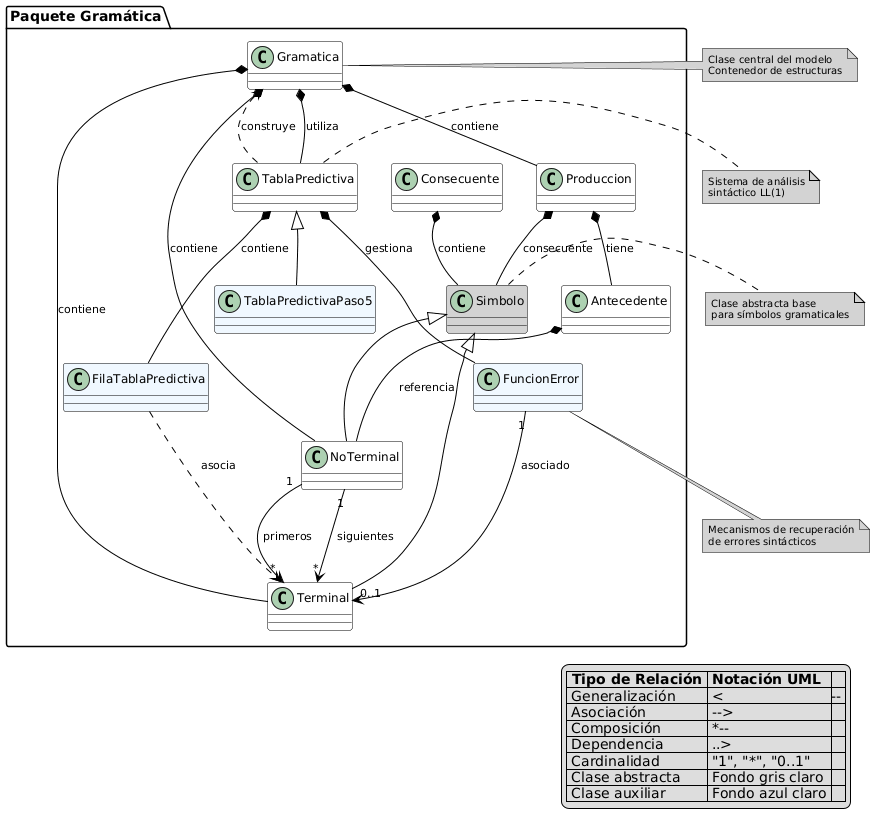
\includegraphics[width=0.9\textwidth]{figuras/Cap9/diagrama_gramatica_bueno.png}
    \caption{Diagrama de clases del paquete gramática - SimAS 3.0}
    \label{fig:diagrama_gramatica}
\end{figure}

\subsubsection{Patrones de diseño en el paquete gramática}

\begin{itemize}
    \item \textbf{Composite}: el patrón Composite se utiliza en la jerarquía de símbolos (Simbolo como componente abstracto, Terminal y NoTerminal como componentes concretos) \cite{gamma1995design}.
    \item \textbf{Observer/Observable}: implementado mediante JavaFX Properties para notificación automática de cambios en la UI cuando se modifican los datos del modelo \cite{gamma1995design}.
    \item \textbf{Strategy}: el patrón Strategy se utiliza en las funciones de error (FuncionError) que encapsulan diferentes estrategias de recuperación de errores \cite{gamma1995design}.
    \item \textbf{Factory Method}: implícito en los constructores de las clases que crean instancias con diferentes configuraciones iniciales \cite{gamma1995design}.
    \item \textbf{Singleton}: la clase Gramatica actúa como contenedor singleton para una gramática específica durante su edición \cite{gamma1995design}.
    \item \textbf{MVC (Model-View-Controller)}: el paquete completo sigue el patrón MVC donde las clases del paquete gramática representan el Modelo, las clases de vistas manejan la presentación, y los controladores coordinan la interacción \cite{burbeck1992applications}.
\end{itemize}

\subsection{Paquete utils}

El paquete \textbf{utils} contiene las clases de utilidad transversales que proporcionan funcionalidades comunes y servicios compartidos utilizados por todos los demás paquetes de SimAS 3.0. Este paquete implementa servicios transversales como gestión de pestañas, internacionalización, monitoreo de componentes y gestión de ventanas secundarias.

Las clases de este paquete permiten:
\begin{itemize}
    \item Gestión avanzada de pestañas y navegación entre ventanas
    \item Sistema completo de internacionalización con soporte multiidioma
    \item Monitoreo y supervisión automática de componentes de la interfaz
    \item Gestión de ventanas secundarias y comunicación entre ellas
    \item Utilidades comunes para todas las capas de la aplicación
\end{itemize}

\subsubsection{Clases del paquete utils}

Este paquete contiene 8 clases principales que proporcionan servicios transversales a toda la aplicación SimAS 3.0, organizadas por funcionalidad: gestión de pestañas, internacionalización, monitoreo y ventanas.

\subsubsection{Clase ActualizableTextos}

La clase \textbf{ActualizableTextos} es una interfaz que define el contrato para la actualización dinámica de textos en la interfaz de usuario cuando cambia el idioma de la aplicación.

\begin{longtable}[H]{|>{\columncolor[rgb]{0.63,0.79,0.95}}m{6cm} | m{8.5cm} |}
\caption{Clase ActualizableTextos - Interfaz de internacionalización}
\endfirsthead
\multicolumn{2}{c}{{\tablename\ \thetable{} -- continúa de la página anterior}} \\
\endhead
\hline \multicolumn{2}{|r|}{{Continúa en la página siguiente}} \\ \hline
\endfoot
\hline
\endlastfoot
\hline
\textbf{Nombre} & \textbf{ActualizableTextos} \\ \hline
\textbf{Descripción} & Interfaz que define el contrato para actualizar textos de la interfaz cuando cambia el idioma, implementada por todas las clases de UI que requieren internacionalización. \\ \hline
\textbf{Métodos} &
\begin{enumerate}
    \item \textbf{actualizarTextos(ResourceBundle)}: método que debe implementar cada clase para actualizar sus textos según el ResourceBundle proporcionado.
\end{enumerate}
\label{tabla_actualizable_textos}
\end{longtable}

\subsubsection{Clase LanguageItem}

La clase \textbf{LanguageItem} representa un elemento de idioma en el sistema de internacionalización, conteniendo información sobre el nombre del idioma, código de localización y bandera correspondiente.

\begin{longtable}[H]{|>{\columncolor[rgb]{0.63,0.79,0.95}}m{6cm} | m{8.5cm} |}
\caption{Clase LanguageItem - Elemento de idioma}
\endfirsthead
\multicolumn{2}{c}{{\tablename\ \thetable{} -- continúa de la página anterior}} \\
\endhead
\hline \multicolumn{2}{|r|}{{Continúa en la página siguiente}} \\ \hline
\endfoot
\hline
\endlastfoot
\hline
\textbf{Nombre} & \textbf{LanguageItem} \\ \hline
\textbf{Descripción} & Representa un idioma disponible en la aplicación, incluyendo su nombre, código de localización y bandera visual para el selector de idiomas. \\ \hline
\textbf{Atributos} &
\begin{enumerate}
    \item \textbf{name}: String con el nombre del idioma (ej: "Español", "English").
    \item \textbf{locale}: String con el código de localización (ej: "es", "en").
    \item \textbf{flagPath}: String con la ruta de la imagen de la bandera.
    \item \textbf{flagImageView}: ImageView que contiene la bandera visual del idioma.
\end{enumerate} \\ \hline
\textbf{Métodos} &
\begin{enumerate}
    \item \textbf{LanguageItem(String, String, String)}: constructor que inicializa el idioma con nombre, localización y ruta de bandera.
    \item \textbf{getName()}: obtiene el nombre del idioma.
    \item \textbf{getLocale()}: obtiene el código de localización.
    \item \textbf{getFlagPath()}: obtiene la ruta de la bandera.
    \item \textbf{getFlagImageView()}: obtiene el ImageView de la bandera.
    \item \textbf{toString()}: devuelve el nombre del idioma como representación textual.
    \item \textbf{equals(Object)}: compara dos LanguageItem por su código de localización.
    \item \textbf{hashCode()}: devuelve el hashCode basado en el código de localización.
\end{enumerate}
\label{tabla_language_item}
\end{longtable}

\subsubsection{Clase LanguageListCell}

La clase \textbf{LanguageListCell} es una celda personalizada para listas de selección de idiomas, que muestra la bandera y nombre del idioma de forma visual.

\begin{longtable}[H]{|>{\columncolor[rgb]{0.63,0.79,0.95}}m{6cm} | m{8.5cm} |}
\caption{Clase LanguageListCell - Celda de lista de idiomas}
\endfirsthead
\multicolumn{2}{c}{{\tablename\ \thetable{} -- continúa de la página anterior}} \\
\endhead
\hline \multicolumn{2}{|r|}{{Continúa en la página siguiente}} \\ \hline
\endfoot
\hline
\endlastfoot
\hline
\textbf{Nombre} & \textbf{LanguageListCell} \\ \hline
\textbf{Descripción} & Celda personalizada para ComboBox y ListView que muestra elementos de idioma con su bandera y nombre de forma visual. \\ \hline
\textbf{Atributos} &
\begin{enumerate}
    \item \textbf{Componentes FXML}: elementos de la interfaz para mostrar bandera y texto.
\end{enumerate} \\ \hline
\textbf{Métodos} &
\begin{enumerate}
    \item \textbf{LanguageListCell()}: constructor que inicializa la celda personalizada.
    \item \textbf{updateItem(LanguageItem, boolean)}: actualiza el contenido visual de la celda con el idioma correspondiente.
    \item \textbf{inicializarComponentes()}: configura los componentes visuales de la celda.
\end{enumerate}
\label{tabla_language_list_cell}
\end{longtable}

\subsubsection{Clase TabManager}

La clase \textbf{TabManager} es el gestor central de pestañas de la aplicación, responsable de crear, gestionar y coordinar todas las pestañas en múltiples ventanas.

\begin{longtable}[H]{|>{\columncolor[rgb]{0.63,0.79,0.95}}m{6cm} | m{8.5cm} |}
\caption{Clase TabManager - Gestor central de pestañas}
\endfirsthead
\multicolumn{2}{c}{{\tablename\ \thetable{} -- continúa de la página anterior}} \\
\endhead
\hline \multicolumn{2}{|r|}{{Continúa en la página siguiente}} \\ \hline
\endfoot
\hline
\endlastfoot
\hline
\textbf{Nombre} & \textbf{TabManager} \\ \hline
\textbf{Descripción} & Gestor central que maneja la creación, gestión y coordinación de todas las pestañas en la aplicación, incluyendo relaciones padre-hijo y grupos de gramáticas. \\ \hline
\textbf{Atributos} &
\begin{enumerate}
    \item \textbf{tabInstances}: Map que almacena instancias de pestañas por TabPane y tipo.
    \item \textbf{parentChildRelations}: Map que mantiene las relaciones padre-hijo entre pestañas.
    \item \textbf{elementoToGrupo}: Map que asocia elementos con sus grupos de gramática.
    \item \textbf{gruposGramatica}: Map que contiene los números de grupo para cada grupo.
    \item \textbf{resourceBundles}: Map que almacena ResourceBundles por TabPane.
    \item \textbf{contadorGrupos}: contador global para generar IDs únicos de grupo.
\end{enumerate} \\ \hline
\textbf{Métodos} &
\begin{enumerate}
    \item \textbf{getOrCreateTab(TabPane, Class, String, Object)}: obtiene o crea una pestaña del tipo especificado.
    \item \textbf{getOrCreateTab(TabPane, Class, String, Object, String, String)}: versión completa con IDs padre-hijo.
    \item \textbf{configurarMenuContextual(TabPane, ResourceBundle)}: configura el menú contextual de las pestañas.
    \item \textbf{reasignarNumerosGrupos(TabPane)}: reasigna números de grupo después de cambios.
    \item \textbf{crearGrupoGramatica(TabPane, String)}: crea un nuevo grupo de gramática.
    \item \textbf{setResourceBundle(TabPane, ResourceBundle)}: establece el ResourceBundle para un TabPane.
    \item \textbf{renumerarGrupos(TabPane)}: renumera todos los grupos de un TabPane.
    \item \textbf{limpiarRelacionesHuérfanas(TabPane)}: limpia relaciones padre-hijo huérfanas.
    \item \textbf{obtenerGruposActivos(TabPane)}: obtiene todos los grupos activos en un TabPane.
    \item \textbf{imprimirEstadoTabPane(TabPane)}: imprime el estado actual de un TabPane para debugging.
\end{enumerate}
\label{tabla_tab_manager}
\end{longtable}

\subsubsection{Clase TabPaneMonitor}

La clase \textbf{TabPaneMonitor} es un monitor singleton que supervisa continuamente el estado de todos los TabPane activos en la aplicación, validando consistencia y reparando automáticamente inconsistencias.

\begin{longtable}[H]{|>{\columncolor[rgb]{0.63,0.79,0.95}}m{6cm} | m{8.5cm} |}
\caption{Clase TabPaneMonitor - Monitor de pestañas}
\endfirsthead
\multicolumn{2}{c}{{\tablename\ \thetable{} -- continúa de la página anterior}} \\
\endhead
\hline \multicolumn{2}{|r|}{{Continúa en la página siguiente}} \\ \hline
\endfoot
\hline
\endlastfoot
\hline
\textbf{Nombre} & \textbf{TabPaneMonitor} \\ \hline
\textbf{Descripción} & Monitor singleton que supervisa continuamente todos los TabPanes activos, validando la consistencia de grupos y relaciones padre-hijo, y reparando automáticamente las inconsistencias detectadas. \\ \hline
\textbf{Atributos} &
\begin{enumerate}
    \item \textbf{instance}: instancia singleton del monitor.
    \item \textbf{monitoredTabPanes}: Map que contiene los TabPanes monitoreados.
    \item \textbf{scheduler}: ScheduledExecutorService para monitoreo periódico.
    \item \textbf{debugMode}: boolean que indica si está en modo debug.
    \item \textbf{movimientoEnProgreso}: boolean que indica si hay un movimiento en progreso.
    \item \textbf{contadorReparaciones}: Map que cuenta las reparaciones por TabPane.
\end{enumerate} \\ \hline
\textbf{Métodos} &
\begin{enumerate}
    \item \textbf{getInstance()}: obtiene la instancia singleton del monitor.
    \item \textbf{registrarTabPane(TabPane, String)}: registra un TabPane para monitoreo.
    \item \textbf{desregistrarTabPane(TabPane)}: desregistra un TabPane del monitoreo.
    \item \textbf{validarConsistenciaGlobal()}: valida la consistencia de todos los TabPanes monitoreados.
    \item \textbf{repararInconsistencias(TabPane, TabPaneInfo)}: repara inconsistencias detectadas.
    \item \textbf{obtenerEstadisticas()}: obtiene estadísticas del monitoreo.
    \item \textbf{setDebugMode(boolean)}: activa o desactiva el modo debug.
    \item \textbf{imprimirEstadoTabPane(TabPane)}: imprime el estado de un TabPane.
    \item \textbf{reiniciarContadores()}: reinicia los contadores de reparaciones.
\end{enumerate} \\ \hline
\textbf{Clase Interna TabPaneInfo} &
\begin{enumerate}
    \item \textbf{TabPaneInfo(TabPane, String)}: constructor de la información de TabPane.
    \item \textbf{tabPane}: referencia al TabPane monitoreado.
    \item \textbf{tabChangeListener}: listener para cambios en pestañas.
    \item \textbf{identifier}: identificador único del TabPane.
    \item \textbf{lastValidation}: timestamp de la última validación.
    \item \textbf{lastKnownGroups}: último estado conocido de grupos.
    \item \textbf{lastKnownRelations}: último estado conocido de relaciones.
\end{enumerate}
\label{tabla_tab_pane_monitor}
\end{longtable}

\subsubsection{Clase SecondaryWindow}

La clase \textbf{SecondaryWindow} extiende EditorWindow para crear ventanas secundarias que permiten trabajar con pestañas de forma independiente de la ventana principal.

\begin{longtable}[H]{|>{\columncolor[rgb]{0.63,0.79,0.95}}m{6cm} | m{8.5cm} |}
\caption{Clase SecondaryWindow - Ventanas secundarias}
\endfirsthead
\multicolumn{2}{c}{{\tablename\ \thetable{} -- continúa de la página anterior}} \\
\endhead
\hline \multicolumn{2}{|r|}{{Continúa en la página siguiente}} \\ \hline
\endfoot
\hline
\endlastfoot
\hline
\textbf{Nombre} & \textbf{SecondaryWindow} \\ \hline
\textbf{Descripción} & Extiende EditorWindow para crear ventanas secundarias que permiten trabajar con pestañas de forma independiente, facilitando la organización del espacio de trabajo. \\ \hline
\textbf{Atributos} &
\begin{enumerate}
    \item \textbf{activeWindows}: Map estático que mantiene todas las ventanas secundarias activas.
    \item \textbf{windowId}: identificador único de la ventana secundaria.
    \item \textbf{localTabPane}: TabPane específico de esta ventana secundaria.
    \item \textbf{stage}: Stage de la ventana secundaria.
    \item \textbf{bundle}: ResourceBundle para internacionalización.
    \item \textbf{windowNumber}: número secuencial de la ventana.
\end{enumerate} \\ \hline
\textbf{Métodos} &
\begin{enumerate}
    \item \textbf{SecondaryWindow(ResourceBundle, String)}: constructor que inicializa la ventana secundaria.
    \item \textbf{getActiveWindows()}: obtiene un mapa con todas las ventanas secundarias activas.
    \item \textbf{initialize()}: inicializa la ventana secundaria con sus componentes.
    \item \textbf{addTabFromDrag(Tab, String)}: añade una pestaña desde un arrastre.
    \item \textbf{setupDragAndDrop()}: configura las funcionalidades de arrastrar y soltar.
    \item \textbf{handleTabClose()}: maneja el cierre de pestañas en la ventana secundaria.
    \item \textbf{updateWindowTitle()}: actualiza el título de la ventana según su contenido.
    \item \textbf{closeWindow()}: cierra la ventana secundaria correctamente.
    \item \textbf{getWindowId()}: obtiene el identificador único de la ventana.
    \item \textbf{getStage()}: obtiene el Stage de la ventana secundaria.
    \item \textbf{getTabPane()}: obtiene el TabPane de la ventana secundaria.
\end{enumerate} \\ \hline
\textbf{Métodos Estáticos} &
\begin{enumerate}
    \item \textbf{getActiveWindows()}: obtiene todas las ventanas secundarias activas.
    \item \textbf{findWindowById(String)}: busca una ventana por su ID.
    \item \textbf{cleanupClosedWindows()}: limpia ventanas cerradas del registro.
\end{enumerate}
\label{tabla_secondary_window}
\end{longtable}

\subsubsection{Dependencias internas del paquete utils}

Las dependencias internas del paquete utils se ilustran en la Figura \ref{fig:diagrama_utils}, donde se puede apreciar la estructura organizada de servicios transversales que proporciona este paquete.

\begin{itemize}
    \item \textbf{TabManager $\leftrightarrow$ TabPaneMonitor}: TabManager utiliza TabPaneMonitor para supervisar los TabPane que gestiona.
    \item \textbf{SecondaryWindow $\rightarrow$ EditorWindow}: SecondaryWindow extiende EditorWindow para crear ventanas independientes.
    \item \textbf{SecondaryWindow $\rightarrow$ TabManager}: SecondaryWindow utiliza TabManager para gestionar sus pestañas.
    \item \textbf{LanguageItem $\leftrightarrow$ LanguageListCell}: LanguageListCell utiliza LanguageItem para mostrar idiomas en listas.
    \item \textbf{ActualizableTextos $\leftarrow$ (todas las clases de UI)}: interfaz implementada por todas las clases que requieren internacionalización.
    \item \textbf{TabManager $\leftrightarrow$ SecondaryWindow}: comunicación bidireccional para gestión de pestañas entre ventanas.
    \item \textbf{Archivos .properties}: todos los archivos de propiedades de idiomas son utilizados por el sistema de internacionalización.
\end{itemize}

\begin{figure}[H]
    \centering
    \includegraphics[width=0.9\textwidth]{figuras/Cap9/diagrama_utils.png}
    \caption{Diagrama de dependencias del paquete utils - SimAS 3.0}
    \label{fig:diagrama_utils}
\end{figure}

\subsubsection{Patrones de diseño en el paquete utils}

\begin{itemize}
    \item \textbf{Singleton}: implementado en TabPaneMonitor para asegurar una única instancia que supervise toda la aplicación \cite{gamma1995design}.
    \item \textbf{Observer}: utilizado en TabPaneMonitor para observar cambios en los TabPane y reaccionar automáticamente \cite{gamma1995design}.
    \item \textbf{Facade}: TabManager actúa como fachada que simplifica la gestión compleja de pestañas y relaciones \cite{gamma1995design}.
    \item \textbf{Factory Method}: implícito en los constructores de TabManager para crear diferentes tipos de pestañas \cite{gamma1995design}.
    \item \textbf{Monitor Object}: TabPaneMonitor implementa el patrón Monitor Object para sincronización segura de acceso a recursos compartidos.
    \item \textbf{Registry}: SecondaryWindow utiliza un registro estático para mantener todas las ventanas secundarias activas.
\end{itemize}

\subsection{Paquete editor}

El paquete \textbf{editor} contiene las clases responsables de la interfaz de usuario para la creación y edición de gramáticas de contexto libre en SimAS 3.0. Este paquete implementa el patrón de diseño MVC donde las clases del editor actúan como controladores que coordinan la interacción entre la vista (componentes JavaFX) y el modelo (paquete gramática).

Las clases de este paquete permiten:
\begin{itemize}
    \item Crear gramáticas mediante un asistente paso a paso
    \item Editar símbolos terminales y no terminales
    \item Gestionar producciones gramaticales
    \item Validar gramáticas creadas
    \item Gestionar múltiples editores en pestañas
    \item Integración completa con el sistema de internacionalización
\end{itemize}

\subsubsection{Clases del paquete editor}

Este paquete contiene 10 clases principales que conforman la interfaz de edición de SimAS 3.0, organizadas jerárquicamente desde la gestión de ventanas hasta los componentes específicos de edición.

\subsubsection{Clase EditorWindow}

La clase \textbf{EditorWindow} representa la ventana principal del editor de gramáticas, gestionando el ciclo de vida de la aplicación de edición y coordinando múltiples pestañas de edición.

\begin{longtable}[H]{|>{\columncolor[rgb]{0.63,0.79,0.95}}m{6cm} | m{8.5cm} |}
\caption{Clase EditorWindow - Ventana principal del editor}
\endfirsthead
\multicolumn{2}{c}{{\tablename\ \thetable{} -- continúa de la página anterior}} \\
\endhead
\hline \multicolumn{2}{|r|}{{Continúa en la página siguiente}} \\ \hline
\endfoot
\hline
\endlastfoot
\hline
\textbf{Nombre} & \textbf{EditorWindow} \\ \hline
\textbf{Descripción} & Gestiona la ventana principal del editor, incluyendo el sistema de pestañas, atajos de teclado y funcionalidades de arrastrar y soltar. \\ \hline
\textbf{Atributos} &
\begin{enumerate}
    \item \textbf{stage}: Stage principal de la ventana del editor.
    \item \textbf{tabPane}: TabPane que contiene todas las pestañas de edición.
    \item \textbf{bundle}: ResourceBundle para internacionalización.
\end{enumerate} \\ \hline
\textbf{Métodos} &
\begin{enumerate}
    \item \textbf{EditorWindow(ResourceBundle)}: constructor que inicializa la ventana con internacionalización.
    \item \textbf{initialize()}: configura la ventana, escena y componentes principales.
    \item \textbf{configurarAtajosTeclado(Scene)}: establece los atajos de teclado globales.
    \item \textbf{show()}: muestra la ventana del editor.
    \item \textbf{close()}: cierra la ventana del editor.
    \item \textbf{addEditorTab(String, Editor)}: añade una nueva pestaña de edición.
    \item \textbf{removeEditorTab(Editor)}: elimina una pestaña de edición.
\end{enumerate}
\label{tabla_editor_window}
\end{longtable}

\subsubsection{Clase Editor}

La clase \textbf{Editor} representa la interfaz principal de edición de una gramática específica, proporcionando acceso a todas las funcionalidades de edición y gestión.

\begin{longtable}[H]{|>{\columncolor[rgb]{0.63,0.79,0.95}}m{6cm} | m{8.5cm} |}
\caption{Clase Editor - Interfaz principal de edición}
\endfirsthead
\multicolumn{2}{c}{{\tablename\ \thetable{} -- continúa de la página anterior}} \\
\endhead
\hline \multicolumn{2}{|r|}{{Continúa en la página siguiente}} \\ \hline
\endfoot
\hline
\endlastfoot
\hline
\textbf{Nombre} & \textbf{Editor} \\ \hline
\textbf{Descripción} & Clase principal que representa un editor de gramáticas, gestionando la interfaz de usuario y la coordinación con el modelo de datos. \\ \hline
\textbf{Atributos} &
\begin{enumerate}
    \item \textbf{gramatica}: instancia de Gramatica que se está editando.
    \item \textbf{tabPane}: referencia al TabPane contenedor.
    \item \textbf{menuPane}: referencia al MenuPrincipal.
    \item \textbf{bundle}: ResourceBundle para internacionalización.
    \item \textbf{editorId}: identificador único del editor.
    \item \textbf{rootPane}: BorderPane raíz de la interfaz.
    \item \textbf{Componentes FXML}: botones, campos de texto, listas, etiquetas.
\end{enumerate} \\ \hline
\textbf{Métodos} &
\begin{enumerate}
    \item \textbf{Editor()}: constructor vacío para carga FXML.
    \item \textbf{Editor(TabPane, MenuPrincipal)}: constructor completo.
    \item \textbf{cargarFXML()}: carga la interfaz desde archivo FXML.
    \item \textbf{inicializarComponentes()}: configura todos los componentes de la UI.
    \item \textbf{configurarEventos()}: establece los manejadores de eventos.
    \item \textbf{actualizarListas()}: actualiza las listas de símbolos y producciones.
    \item \textbf{btnAnadir\_action()}: maneja la acción de añadir nueva gramática.
    \item \textbf{btnAbrir\_action()}: maneja la apertura de gramáticas existentes.
    \item \textbf{btnGuardar\_action()}: maneja el guardado de gramáticas.
    \item \textbf{btnEditar\_action()}: activa el modo de edición.
    \item \textbf{btnEliminar\_action()}: elimina la gramática actual.
    \item \textbf{btnValidar\_action()}: valida la gramática.
    \item \textbf{btnInforme\_action()}: genera informes de la gramática.
    \item \textbf{btnSimular\_action()}: inicia la simulación.
    \item \textbf{btnSalir\_action()}: cierra el editor.
    \item \textbf{actualizarTextos(ResourceBundle)}: actualiza textos para internacionalización.
\end{enumerate} \\ \hline
\textbf{Métodos} &
\begin{enumerate}
    \item \textbf{getGramatica()}: obtiene la gramática actual.
    \item \textbf{setGramatica(Gramatica)}: establece una nueva gramática.
    \item \textbf{getBundle()}: obtiene el ResourceBundle.
    \item \textbf{configurarRelacionesPadreHijo()}: configura el sistema de identificación.
    \item \textbf{crearGramatica()}: crea una nueva instancia de Gramatica.
\end{enumerate}
\label{tabla_editor}
\end{longtable}

\subsubsection{Clase PanelCreacionGramatica}

La clase \textbf{PanelCreacionGramatica} coordina el asistente de creación de gramáticas paso a paso, gestionando la navegación entre los diferentes pasos del proceso.

\begin{longtable}[H]{|>{\columncolor[rgb]{0.63,0.79,0.95}}m{6cm} | m{8.5cm} |}
\caption{Clase PanelCreacionGramatica - Asistente de creación}
\endfirsthead
\multicolumn{2}{c}{{\tablename\ \thetable{} -- continúa de la página anterior}} \\
\endhead
\hline \multicolumn{2}{|r|}{{Continúa en la página siguiente}} \\ \hline
\endfoot
\hline
\endlastfoot
\hline
\textbf{Nombre} & \textbf{PanelCreacionGramatica} \\ \hline
\textbf{Descripción} & Coordina el asistente paso a paso para la creación de gramáticas, gestionando la navegación y el flujo de datos entre los diferentes paneles. \\ \hline
\textbf{Atributos} &
\begin{enumerate}
    \item \textbf{tabPane}: TabPane contenedor de las pestañas.
    \item \textbf{paso1-4}: instancias de los paneles de cada paso del asistente.
    \item \textbf{panelPadre}: referencia al Editor padre.
    \item \textbf{menuPane}: referencia al MenuPrincipal.
    \item \textbf{gramaticaTemporal}: copia temporal de la gramática en edición.
    \item \textbf{bundle}: ResourceBundle para internacionalización.
    \item \textbf{creacionId}: identificador único del proceso de creación.
\end{enumerate} \\ \hline
\textbf{Métodos} &
\begin{enumerate}
    \item \textbf{PanelCreacionGramatica(Editor, TabPane, Gramatica, MenuPrincipal)}: constructor principal.
    \item \textbf{inicializarPaneles()}: inicializa todos los paneles del asistente.
    \item \textbf{configurarNavegacion()}: configura la navegación entre pasos.
    \item \textbf{validarPasoActual()}: valida el contenido del paso actual.
    \item \textbf{avanzarAlSiguientePaso()}: navega al siguiente paso del asistente.
    \item \textbf{retrocederAlPasoAnterior()}: navega al paso anterior.
    \item \textbf{finalizarCreacion()}: completa el proceso de creación.
    \item \textbf{cancelarCreacion()}: cancela el proceso de creación.
    \item \textbf{actualizarGramaticaTemporal()}: actualiza la gramática temporal con los datos actuales.
    \item \textbf{actualizarTextos(ResourceBundle)}: actualiza textos para internacionalización.
\end{enumerate}
\label{tabla_panel_creacion_gramatica}
\end{longtable}

\subsubsection{Clase PanelCreacionGramaticaPaso1}

La clase \textbf{PanelCreacionGramaticaPaso1} maneja el primer paso del asistente de creación, donde se definen los metadatos básicos de la gramática.

\begin{longtable}[H]{|>{\columncolor[rgb]{0.63,0.79,0.95}}m{6cm} | m{8.5cm} |}
\caption{Clase PanelCreacionGramaticaPaso1 - Paso 1: Metadatos}
\endfirsthead
\multicolumn{2}{c}{{\tablename\ \thetable{} -- continúa de la página anterior}} \\
\endhead
\hline \multicolumn{2}{|r|}{{Continúa en la página siguiente}} \\ \hline
\endfoot
\hline
\endlastfoot
\hline
\textbf{Nombre} & \textbf{PanelCreacionGramaticaPaso1} \\ \hline
\textbf{Descripción} & Primer paso del asistente de creación de gramáticas, donde se definen el nombre, descripción y símbolo inicial. \\ \hline
\textbf{Atributos} &
\begin{enumerate}
    \item \textbf{panelPadre}: referencia al PanelCreacionGramatica padre.
    \item \textbf{bundle}: ResourceBundle para internacionalización.
    \item \textbf{Componentes FXML}: campos de texto para nombre, descripción y símbolo inicial.
    \item \textbf{btnSiguiente}: botón para avanzar al siguiente paso.
    \item \textbf{btnCancelar}: botón para cancelar la creación.
\end{enumerate} \\ \hline
\textbf{Métodos} &
\begin{enumerate}
    \item \textbf{PanelCreacionGramaticaPaso1( PanelCreacionGramatica, ResourceBundle)}: constructor.
    \item \textbf{inicializarInterfaz()}: configura la interfaz del paso 1.
    \item \textbf{configurarValidacion()}: establece las reglas de validación.
    \item \textbf{setNombre(String)}: establece el nombre de la gramática.
    \item \textbf{setDescripcion(String)}: establece la descripción.
    \item \textbf{setSimboloInicial(String)}: establece el símbolo inicial.
    \item \textbf{validarCampos()}: valida que todos los campos requeridos estén completos.
    \item \textbf{btnSiguiente\_action()}: maneja el avance al siguiente paso.
    \item \textbf{btnCancelar\_action()}: maneja la cancelación.
    \item \textbf{actualizarTextos(ResourceBundle)}: actualiza textos para internacionalización.
\end{enumerate}
\label{tabla_panel_creacion_paso1}
\end{longtable}

\subsubsection{Clase PanelCreacionGramaticaPaso2}

La clase \textbf{PanelCreacionGramaticaPaso2} maneja el segundo paso del asistente de creación, donde se definen los símbolos terminales y no terminales.

\begin{longtable}[H]{|>{\columncolor[rgb]{0.63,0.79,0.95}}m{6cm} | m{8.5cm} |}
\caption{Clase PanelCreacionGramaticaPaso2 - Paso 2: Símbolos}
\endfirsthead
\multicolumn{2}{c}{{\tablename\ \thetable{} -- continúa de la página anterior}} \\
\endhead
\hline \multicolumn{2}{|r|}{{Continúa en la página siguiente}} \\ \hline
\endfoot
\hline
\endlastfoot
\hline
\textbf{Nombre} & \textbf{PanelCreacionGramaticaPaso2} \\ \hline
\textbf{Descripción} & Segundo paso del asistente donde se definen y gestionan los símbolos terminales y no terminales de la gramática. \\ \hline
\textbf{Atributos} &
\begin{enumerate}
    \item \textbf{panelPadre}: referencia al PanelCreacionGramatica padre.
    \item \textbf{menuPane}: referencia al MenuPrincipal.
    \item \textbf{tabPane}: TabPane para gestión de pestañas.
    \item \textbf{panelTerminales}: PanelSimbolosTerminales para gestión de terminales.
    \item \textbf{panelNoTerminales}: PanelSimbolosNoTerminales para gestión de no terminales.
    \item \textbf{bundle}: ResourceBundle para internacionalización.
    \item \textbf{btnSiguiente, btnAnterior, btnCancelar}: botones de navegación.
\end{enumerate} \\ \hline
\textbf{Métodos} &
\begin{enumerate}
    \item \textbf{PanelCreacionGramaticaPaso2( PanelCreacionGramatica, MenuPrincipal, TabPane)}: constructor.
    \item \textbf{inicializarPaneles()}: inicializa los paneles de símbolos.
    \item \textbf{configurarNavegacion()}: configura los botones de navegación.
    \item \textbf{validarSimbolos()}: valida que los símbolos definidos sean correctos.
    \item \textbf{asignarListaSimbolosTerminales( ObservableList<String>)}: asigna la lista de terminales.
    \item \textbf{asignarListaSimbolosNoTerminales( ObservableList<String>)}: asigna la lista de no terminales.
    \item \textbf{obtenerSimbolosTerminales()}: obtiene los símbolos terminales definidos.
    \item \textbf{obtenerSimbolosNoTerminales()}: obtiene los símbolos no terminales definidos.
    \item \textbf{btnSiguiente\_action()}: maneja el avance al siguiente paso.
    \item \textbf{btnAnterior\_action()}: maneja el retroceso al paso anterior.
    \item \textbf{btnCancelar\_action()}: maneja la cancelación.
    \item \textbf{actualizarTextos(ResourceBundle)}: actualiza textos para internacionalización.
\end{enumerate}
\label{tabla_panel_creacion_paso2}
\end{longtable}

\subsubsection{Clase PanelCreacionGramaticaPaso3}

La clase \textbf{PanelCreacionGramaticaPaso3} maneja el tercer paso del asistente, donde se definen las producciones de la gramática.

\begin{longtable}[H]{|>{\columncolor[rgb]{0.63,0.79,0.95}}m{6cm} | m{8.5cm} |}
\caption{Clase PanelCreacionGramaticaPaso3 - Paso 3: Producciones}
\endfirsthead
\multicolumn{2}{c}{{\tablename\ \thetable{} -- continúa de la página anterior}} \\
\endhead
\hline \multicolumn{2}{|r|}{{Continúa en la página siguiente}} \\ \hline
\endfoot
\hline
\endlastfoot
\hline
\textbf{Nombre} & \textbf{PanelCreacionGramaticaPaso3} \\ \hline
\textbf{Descripción} & Tercer paso del asistente donde se definen y gestionan las producciones de la gramática. \\ \hline
\textbf{Atributos} &
\begin{enumerate}
    \item \textbf{panelPadre}: referencia al PanelCreacionGramatica padre.
    \item \textbf{tabPane}: TabPane para gestión de pestañas.
    \item \textbf{menuPane}: referencia al MenuPrincipal.
    \item \textbf{panelProducciones}: PanelProducciones para gestión de producciones.
    \item \textbf{bundle}: ResourceBundle para internacionalización.
    \item \textbf{btnSiguiente, btnAnterior, btnCancelar}: botones de navegación.
\end{enumerate} \\ \hline
\textbf{Métodos} &
\begin{enumerate}
    \item \textbf{PanelCreacionGramaticaPaso3( PanelCreacionGramatica, TabPane, MenuPrincipal)}: constructor.
    \item \textbf{inicializarPanelProducciones()}: inicializa el panel de producciones.
    \item \textbf{configurarNavegacion()}: configura los botones de navegación.
    \item \textbf{validarProducciones()}: valida que las producciones definidas sean correctas.
    \item \textbf{asignarProducciones( ObservableList<Produccion>)}: asigna las producciones existentes.
    \item \textbf{obtenerProducciones()}: obtiene las producciones definidas.
    \item \textbf{btnSiguiente\_action()}: maneja el avance al siguiente paso.
    \item \textbf{btnAnterior\_action()}: maneja el retroceso al paso anterior.
    \item \textbf{btnCancelar\_action()}: maneja la cancelación.
    \item \textbf{actualizarTextos(ResourceBundle)}: actualiza textos para internacionalización.
\end{enumerate}
\label{tabla_panel_creacion_paso3}
\end{longtable}

\subsubsection{Clase PanelCreacionGramaticaPaso4}

La clase \textbf{PanelCreacionGramaticaPaso4} maneja el cuarto y último paso del asistente, donde se realiza la validación final y se completa la creación.

\begin{longtable}[H]{|>{\columncolor[rgb]{0.63,0.79,0.95}}m{6cm} | m{8.5cm} |}
\caption{Clase PanelCreacionGramaticaPaso4 - Paso 4: Validación}
\endfirsthead
\multicolumn{2}{c}{{\tablename\ \thetable{} -- continúa de la página anterior}} \\
\endhead
\hline \multicolumn{2}{|r|}{{Continúa en la página siguiente}} \\ \hline
\endfoot
\hline
\endlastfoot
\hline
\textbf{Nombre} & \textbf{PanelCreacionGramaticaPaso4} \\ \hline
\textbf{Descripción} & Cuarto y último paso del asistente donde se elige el símbolo inicial y se finaliza el proceso de creación. \\ \hline
\textbf{Atributos} &
\begin{enumerate}
    \item \textbf{panelPadre}: referencia al PanelCreacionGramatica padre.
    \item \textbf{tabPane}: TabPane para gestión de pestañas.
    \item \textbf{bundle}: ResourceBundle para internacionalización.
    \item \textbf{Componentes FXML}: etiquetas, botones de finalizar y cancelar.
    \item \textbf{areaValidacion}: área de texto para mostrar resultados de validación.
\end{enumerate} \\ \hline
\textbf{Métodos} &
\begin{enumerate}
    \item \textbf{PanelCreacionGramaticaPaso4( PanelCreacionGramatica, TabPane)}: constructor.
    \item \textbf{inicializarInterfaz()}: configura la interfaz del paso final.
    \item \textbf{realizarValidacionFinal()}: ejecuta todas las validaciones de la gramática.
    \item \textbf{mostrarResultadosValidacion()}: muestra los resultados de la validación.
    \item \textbf{btnFinalizar\_action()}: maneja la finalización exitosa del asistente.
    \item \textbf{btnVolver\_action()}: permite volver a pasos anteriores para correcciones.
    \item \textbf{btnCancelar\_action()}: maneja la cancelación completa.
    \item \textbf{generarResumenGramatica()}: genera un resumen de la gramática creada.
    \item \textbf{actualizarTextos(ResourceBundle)}: actualiza textos para internacionalización.
\end{enumerate}
\label{tabla_panel_creacion_paso4}
\end{longtable}

\subsubsection{Clase PanelProducciones}

La clase \textbf{PanelProducciones} proporciona la interfaz para editar y gestionar las producciones de la gramática.

\begin{longtable}[H]{|>{\columncolor[rgb]{0.63,0.79,0.95}}m{6cm} | m{8.5cm} |}
\caption{Clase PanelProducciones - Gestión de producciones}
\endfirsthead
\multicolumn{2}{c}{{\tablename\ \thetable{} -- continúa de la página anterior}} \\
\endhead
\hline \multicolumn{2}{|r|}{{Continúa en la página siguiente}} \\ \hline
\endfoot
\hline
\endlastfoot
\hline
\textbf{Nombre} & \textbf{PanelProducciones} \\ \hline
\textbf{Descripción} & Panel especializado para la creación, edición y eliminación de producciones gramaticales. \\ \hline
\textbf{Atributos} &
\begin{enumerate}
    \item \textbf{panelPadre}: referencia al PanelCreacionGramaticaPaso3 padre.
    \item \textbf{tabPane}: TabPane para gestión de pestañas.
    \item \textbf{producciones}: ObservableList de producciones.
    \item \textbf{noTerminales}: ObservableList de símbolos no terminales disponibles.
    \item \textbf{terminales}: ObservableList de símbolos terminales disponibles.
    \item \textbf{bundle}: ResourceBundle para internacionalización.
    \item \textbf{Componentes FXML}: ComboBox, TextField, ListViews, Buttons, Labels.
\end{enumerate} \\ \hline
\textbf{Métodos} &
\begin{enumerate}
    \item \textbf{PanelProducciones( PanelCreacionGramaticaPaso3, ObservableList<Produccion>, TabPane)}: constructor.
    \item \textbf{cargarFXML()}: carga la interfaz desde archivo FXML.
    \item \textbf{inicializarComponentes()}: configura todos los componentes de la UI.
    \item \textbf{configurarEventos()}: establece los manejadores de eventos.
    \item \textbf{actualizarListasSimbolos()}: actualiza las listas de símbolos disponibles.
    \item \textbf{btnInsertar\_action()}: inserta una nueva producción.
    \item \textbf{btnModificar\_action()}: modifica la producción seleccionada.
    \item \textbf{btnEliminar\_action()}: elimina la producción seleccionada.
    \item \textbf{btnBorrar\_action()}: borra el contenido del campo de consecuente.
    \item \textbf{btnEpsilon\_action()}: inserta el símbolo épsilon.
    \item \textbf{btnCancelar\_action()}: cancela la operación actual.
    \item \textbf{btnAceptar\_action()}: acepta y guarda los cambios.
    \item \textbf{validarProduccion()}: valida que la producción sea correcta.
    \item \textbf{actualizarTextos(ResourceBundle)}: actualiza textos para internacionalización.
\end{enumerate}
\label{tabla_panel_producciones}
\end{longtable}

\subsubsection{Clase PanelSimbolosTerminales}

La clase \textbf{PanelSimbolosTerminales} proporciona la interfaz para gestionar los símbolos terminales de la gramática.

\begin{longtable}[H]{|>{\columncolor[rgb]{0.63,0.79,0.95}}m{6cm} | m{8.5cm} |}
\caption{Clase PanelSimbolosTerminales - Gestión de terminales}
\endfirsthead
\multicolumn{2}{c}{{\tablename\ \thetable{} -- continúa de la página anterior}} \\
\endhead
\hline \multicolumn{2}{|r|}{{Continúa en la página siguiente}} \\ \hline
\endfoot
\hline
\endlastfoot
\hline
\textbf{Nombre} & \textbf{PanelSimbolosTerminales} \\ \hline
\textbf{Descripción} & Panel especializado para la gestión de símbolos terminales, incluyendo símbolos predefinidos y personalizados. \\ \hline
\textbf{Atributos} &
\begin{enumerate}
    \item \textbf{panelPadre}: referencia al PanelCreacionGramaticaPaso2 padre.
    \item \textbf{tabPane}: TabPane para gestión de pestañas.
    \item \textbf{simbolosTerminales}: ObservableList de símbolos terminales.
    \item \textbf{simbolosTemporales}: copia temporal de los símbolos.
    \item \textbf{simbolosSet}: Set para validación de unicidad.
    \item \textbf{bundle}: ResourceBundle para internacionalización.
    \item \textbf{simbolosPredefinidos}: array de símbolos comunes predefinidos.
    \item \textbf{Componentes FXML}: FlowPane, TextField, ListView, Buttons, Labels.
\end{enumerate} \\ \hline
\textbf{Métodos} &
\begin{enumerate}
    \item \textbf{PanelSimbolosTerminales( ObservableList<String>, TabPane, PanelCreacionGramaticaPaso2)}: constructor.
    \item \textbf{cargarFXML()}: carga la interfaz desde archivo FXML.
    \item \textbf{inicializarComponentes()}: configura todos los componentes de la UI.
    \item \textbf{crearBotonesPredefinidos()}: crea botones para símbolos predefinidos.
    \item \textbf{configurarEventos()}: establece los manejadores de eventos.
    \item \textbf{actualizarListaSimbolos()}: actualiza la lista visual de símbolos.
    \item \textbf{btnInsertar\_action()}: inserta un nuevo símbolo terminal.
    \item \textbf{btnModificar\_action()}: modifica el símbolo seleccionado.
    \item \textbf{btnEliminar\_action()}: elimina el símbolo seleccionado.
    \item \textbf{btnCancelar\_action()}: cancela la operación actual.
    \item \textbf{btnAceptar\_action()}: acepta y guarda los cambios.
    \item \textbf{validarSimbolo()}: valida que el símbolo sea único y válido.
    \item \textbf{actualizarTextos(ResourceBundle)}: actualiza textos para internacionalización.
\end{enumerate}
\label{tabla_panel_simbolos_terminales}
\end{longtable}

\subsubsection{Clase PanelSimbolosNoTerminales}

La clase \textbf{PanelSimbolosNoTerminales} proporciona la interfaz para gestionar los símbolos no terminales de la gramática.

\begin{longtable}[H]{|>{\columncolor[rgb]{0.63,0.79,0.95}}m{6cm} | m{8.5cm} |}
\caption{Clase PanelSimbolosNoTerminales - Gestión de no terminales}
\endfirsthead
\multicolumn{2}{c}{{\tablename\ \thetable{} -- continúa de la página anterior}} \\
\endhead
\hline \multicolumn{2}{|r|}{{Continúa en la página siguiente}} \\ \hline
\endfoot
\hline
\endlastfoot
\hline
\textbf{Nombre} & \textbf{PanelSimbolosNoTerminales} \\ \hline
\textbf{Descripción} & Panel especializado para la gestión de símbolos no terminales de la gramática. \\ \hline
\textbf{Atributos} &
\begin{enumerate}
    \item \textbf{panelPadre}: referencia al PanelCreacionGramaticaPaso2 padre.
    \item \textbf{tabPane}: TabPane para gestión de pestañas.
    \item \textbf{simbolosNoTerminales}: ObservableList de símbolos no terminales.
    \item \textbf{simbolosTemporales}: copia temporal de los símbolos.
    \item \textbf{simbolosSet}: Set para validación de unicidad.
    \item \textbf{bundle}: ResourceBundle para internacionalización.
    \item \textbf{Componentes FXML}: TextField, ListView, Buttons, Labels.
\end{enumerate} \\ \hline
\textbf{Métodos} &
\begin{enumerate}
    \item \textbf{PanelSimbolosNoTerminales( ObservableList<String>, TabPane, PanelCreacionGramaticaPaso2)}: constructor.
    \item \textbf{cargarFXML()}: carga la interfaz desde archivo FXML.
    \item \textbf{inicializarComponentes()}: configura todos los componentes de la UI.
    \item \textbf{configurarEventos()}: establece los manejadores de eventos.
    \item \textbf{actualizarListaSimbolos()}: actualiza la lista visual de símbolos.
    \item \textbf{btnInsertar\_action()}: inserta un nuevo símbolo no terminal.
    \item \textbf{btnModificar\_action()}: modifica el símbolo seleccionado.
    \item \textbf{btnEliminar\_action()}: elimina el símbolo seleccionado.
    \item \textbf{btnCancelar\_action()}: cancela la operación actual.
    \item \textbf{btnAceptar\_action()}: acepta y guarda los cambios.
    \item \textbf{validarSimbolo()}: valida que el símbolo sea único y válido.
    \item \textbf{actualizarTextos(ResourceBundle)}: actualiza textos para internacionalización.
\end{enumerate}
\label{tabla_panel_simbolos_no_terminales}
\end{longtable}

\subsubsection{Dependencias internas del paquete editor}

Las dependencias internas del paquete editor se ilustran en la Figura \ref{fig:diagrama_editor}, donde se puede apreciar la estructura jerárquica del asistente de creación y las relaciones entre los diferentes componentes de la interfaz.

\begin{itemize}
    \item \textbf{EditorWindow $\rightarrow$ Editor}: EditorWindow crea y gestiona múltiples instancias de Editor.
    \item \textbf{Editor $\rightarrow$ PanelCreacionGramatica}: Editor utiliza PanelCreacionGramatica para el asistente de creación.
    \item \textbf{PanelCreacionGramatica $\rightarrow$ PanelCreacionGramaticaPaso1-4}: PanelCreacionGramatica coordina los cuatro pasos del asistente.
    \item \textbf{PanelCreacionGramaticaPaso2 $\rightarrow$ PanelSimbolosTerminales, PanelSimbolosNoTerminales}: Paso 2 utiliza paneles específicos para gestión de símbolos.
    \item \textbf{PanelCreacionGramaticaPaso3 $\rightarrow$ PanelProducciones}: Paso 3 utiliza PanelProducciones para gestión de producciones.
    \item \textbf{PanelProducciones $\rightarrow$ gramatica.Gramatica}: PanelProducciones accede a la gramática para obtener símbolos disponibles.
    \item \textbf{PanelSimbolosTerminales $\rightarrow$ gramatica.Terminal}: PanelSimbolosTerminales gestiona símbolos terminales.
    \item \textbf{PanelSimbolosNoTerminales $\rightarrow$ gramatica.NoTerminal}: PanelSimbolosNoTerminales gestiona símbolos no terminales.
    \item \textbf{Todas las clases $\rightarrow$ utils.ActualizableTextos}: todas las clases del editor implementan esta interfaz para internacionalización.
    \item \textbf{Todas las clases $\rightarrow$ bienvenida.MenuPrincipal}: acceso al menú principal para navegación.
    \item \textbf{Todas las clases $\rightarrow$ utils.TabManager}: gestión de pestañas y grupos de gramáticas.
\end{itemize}

\subsubsection{Patrones de diseño en el paquete editor}

\begin{itemize}
    \item \textbf{MVC (Model-View-Controller)}: las clases del editor actúan como controladores coordinando entre las vistas JavaFX y el modelo gramática \cite{burbeck1992applications}.
    \item \textbf{Observer}: implementado mediante JavaFX Properties para notificación automática de cambios en la UI \cite{gamma1995design}.
    \item \textbf{Strategy}: los diferentes paneles (PanelProducciones, PanelSimbolosTerminales, etc.) implementan estrategias específicas de edición \cite{gamma1995design}.
    \item \textbf{Factory Method}: los constructores de las clases crean instancias con diferentes configuraciones iniciales \cite{gamma1995design}.
    \item \textbf{Composite}: la estructura jerárquica de paneles (PanelCreacionGramatica conteniendo PanelCreacionGramaticaPaso1-4) \cite{gamma1995design}.
    \item \textbf{Singleton}: uso implícito en la gestión de recursos compartidos como ResourceBundle \cite{gamma1995design}.
\end{itemize}

\begin{figure}[p]
    \centering
    \includegraphics[angle=90,width=0.95\textwidth]{figuras/Cap9/diagrama_editor.png}
    \caption{Diagrama de clases del paquete editor - SimAS 3.0}
    \label{fig:diagrama_editor}
\end{figure}

\subsection{Paquete simulador}

El paquete \textbf{simulador} contiene las clases responsables de la simulación del análisis sintáctico descendente en SimAS 3.0. Este paquete implementa el núcleo funcional de la aplicación, permitiendo a los usuarios simular paso a paso el proceso de análisis sintáctico de cadenas de entrada utilizando gramáticas libres de contexto.

Las clases de este paquete permiten:
\begin{itemize}
    \item Simulación completa del análisis sintáctico descendente
    \item Visualización paso a paso del proceso de análisis
    \item Gestión de funciones de error y recuperación
    \item Creación y edición de cadenas de entrada
    \item Interfaz interactiva para la simulación
    \item Generación de informes y árboles de derivación
\end{itemize}

\subsubsection{Clases del paquete simulador}

Este paquete contiene 13 clases principales que implementan el sistema completo de simulación de análisis sintáctico, organizadas por funcionalidad: clases principales de simulación, pasos de la simulación descendente y componentes auxiliares.

\subsubsection{Clase PanelNuevaSimDescPaso}

La clase \textbf{PanelNuevaSimDescPaso} es una interfaz que define el contrato que deben implementar todos los pasos de la simulación descendente.

\begin{longtable}[H]{|>{\columncolor[rgb]{0.63,0.79,0.95}}m{6cm} | m{8.5cm} |}
\caption{Clase PanelNuevaSimDescPaso - Interfaz de pasos de simulación}
\endfirsthead
\multicolumn{2}{c}{{\tablename\ \thetable{} -- continúa de la página anterior}} \\
\endhead
\hline \multicolumn{2}{|r|}{{Continúa en la página siguiente}} \\ \hline
\endfoot
\hline
\endlastfoot
\hline
\textbf{Nombre} & \textbf{PanelNuevaSimDescPaso} \\ \hline
\textbf{Descripción} & Interfaz que define el contrato para todos los pasos de la simulación descendente, asegurando consistencia en la implementación. \\ \hline
\textbf{Métodos} &
\begin{enumerate}
    \item \textbf{getRoot()}: retorna el nodo raíz del paso de simulación.
\end{enumerate}
\label{tabla_panel_nueva_sim_desc_paso}
\end{longtable}

\subsubsection{Clase PanelNuevaSimDescPaso1}

La clase \textbf{PanelNuevaSimDescPaso1} implementa el primer paso de la simulación descendente, mostrando la gramática original y permitiendo la navegación entre pasos.

\begin{longtable}[H]{|>{\columncolor[rgb]{0.63,0.79,0.95}}m{6cm} | m{8.5cm} |}
\caption{Clase PanelNuevaSimDescPaso1 - Paso 1 de simulación}
\endfirsthead
\multicolumn{2}{c}{{\tablename\ \thetable{} -- continúa de la página anterior}} \\
\endhead
\hline \multicolumn{2}{|r|}{{Continúa en la página siguiente}} \\ \hline
\endfoot
\hline
\endlastfoot
\hline
\textbf{Nombre} & \textbf{PanelNuevaSimDescPaso1} \\ \hline
\textbf{Descripción} & Implementa el primer paso de la simulación descendente, mostrando la gramática original y permitiendo navegación entre los diferentes pasos del proceso. \\ \hline
\textbf{Atributos} &
\begin{enumerate}
    \item \textbf{panelPadre}: PanelSimuladorDesc que contiene este paso.
    \item \textbf{gramatica}: Gramatica que se está simulando.
    \item \textbf{bundle}: ResourceBundle para internacionalización.
    \item \textbf{root}: Parent que representa la interfaz gráfica del paso.
\end{enumerate} \\ \hline
\textbf{Métodos} &
\begin{enumerate}
    \item \textbf{PanelNuevaSimDescPaso1( PanelSimuladorDesc)}: constructor que inicializa el paso con su panel padre.
    \item \textbf{getRoot()}: retorna el nodo raíz de la interfaz gráfica.
    \item \textbf{actualizarTextos(ResourceBundle)}: actualiza los textos según el idioma seleccionado.
    \item \textbf{cargarFXML()}: carga el archivo FXML correspondiente al paso.
    \item \textbf{inicializarBotones()}: configura los botones de navegación.
\end{enumerate}
\label{tabla_panel_nueva_sim_desc_paso1}
\end{longtable}

\subsubsection{Clase PanelNuevaSimDescPaso2}

La clase \textbf{PanelNuevaSimDescPaso2} implementa el segundo paso de la simulación descendente, mostrando los símbolos terminales y no terminales.

\begin{longtable}[H]{|>{\columncolor[rgb]{0.63,0.79,0.95}}m{6cm} | m{8.5cm} |}
\caption{Clase PanelNuevaSimDescPaso2 - Paso 2 de simulación}
\endfirsthead
\multicolumn{2}{c}{{\tablename\ \thetable{} -- continúa de la página anterior}} \\
\endhead
\hline \multicolumn{2}{|r|}{{Continúa en la página siguiente}} \\ \hline
\endfoot
\hline
\endlastfoot
\hline
\textbf{Nombre} & \textbf{PanelNuevaSimDescPaso2} \\ \hline
\textbf{Descripción} & Implementa el segundo paso de la simulación descendente, mostrando los símbolos terminales y no terminales de la gramática. \\ \hline
\textbf{Atributos} &
\begin{enumerate}
    \item \textbf{panelPadre}: PanelSimuladorDesc que contiene este paso.
    \item \textbf{gramatica}: Gramatica que se está simulando.
    \item \textbf{bundle}: ResourceBundle para internacionalización.
    \item \textbf{root}: Parent que representa la interfaz gráfica del paso.
\end{enumerate} \\ \hline
\textbf{Métodos} &
\begin{enumerate}
    \item \textbf{PanelNuevaSimDescPaso2( PanelSimuladorDesc)}: constructor que inicializa el paso con su panel padre.
    \item \textbf{getRoot()}: retorna el nodo raíz de la interfaz gráfica.
    \item \textbf{actualizarTextos(ResourceBundle)}: actualiza los textos según el idioma seleccionado.
\end{enumerate}
\label{tabla_panel_nueva_sim_desc_paso2}
\end{longtable}

\subsubsection{Clase PanelNuevaSimDescPaso3}

La clase \textbf{PanelNuevaSimDescPaso3} implementa el tercer paso de la simulación descendente, mostrando los conjuntos First y Follow.

\begin{longtable}[H]{|>{\columncolor[rgb]{0.63,0.79,0.95}}m{6cm} | m{8.5cm} |}
\caption{Clase PanelNuevaSimDescPaso3 - Paso 3 de simulación}
\endfirsthead
\multicolumn{2}{c}{{\tablename\ \thetable{} -- continúa de la página anterior}} \\
\endhead
\hline \multicolumn{2}{|r|}{{Continúa en la página siguiente}} \\ \hline
\endfoot
\hline
\endlastfoot
\hline
\textbf{Nombre} & \textbf{PanelNuevaSimDescPaso3} \\ \hline
\textbf{Descripción} & Implementa el tercer paso de la simulación descendente, mostrando los conjuntos First y Follow de los símbolos no terminales. \\ \hline
\textbf{Atributos} &
\begin{enumerate}
    \item \textbf{panelPadre}: PanelSimuladorDesc que contiene este paso.
    \item \textbf{gramatica}: Gramatica que se está simulando.
    \item \textbf{bundle}: ResourceBundle para internacionalización.
    \item \textbf{root}: Parent que representa la interfaz gráfica del paso.
\end{enumerate} \\ \hline
\textbf{Métodos} &
\begin{enumerate}
    \item \textbf{PanelNuevaSimDescPaso3( PanelSimuladorDesc)}: constructor que inicializa el paso con su panel padre.
    \item \textbf{getRoot()}: retorna el nodo raíz de la interfaz gráfica.
    \item \textbf{actualizarTextos(ResourceBundle)}: actualiza los textos según el idioma seleccionado.
\end{enumerate}
\label{tabla_panel_nueva_sim_desc_paso3}
\end{longtable}

\subsubsection{Clase PanelNuevaSimDescPaso4}

La clase \textbf{PanelNuevaSimDescPaso4} implementa el cuarto paso de la simulación descendente, mostrando la tabla predictiva.

\begin{longtable}[H]{|>{\columncolor[rgb]{0.63,0.79,0.95}}m{6cm} | m{8.5cm} |}
\caption{Clase PanelNuevaSimDescPaso4 - Paso 4 de simulación}
\endfirsthead
\multicolumn{2}{c}{{\tablename\ \thetable{} -- continúa de la página anterior}} \\
\endhead
\hline \multicolumn{2}{|r|}{{Continúa en la página siguiente}} \\ \hline
\endfoot
\hline
\endlastfoot
\hline
\textbf{Nombre} & \textbf{PanelNuevaSimDescPaso4} \\ \hline
\textbf{Descripción} & Implementa el cuarto paso de la simulación descendente, mostrando la tabla predictiva completa con sus celdas y funciones de error. \\ \hline
\textbf{Atributos} &
\begin{enumerate}
    \item \textbf{panelPadre}: PanelSimuladorDesc que contiene este paso.
    \item \textbf{gramatica}: Gramatica que se está simulando.
    \item \textbf{bundle}: ResourceBundle para internacionalización.
    \item \textbf{root}: Parent que representa la interfaz gráfica del paso.
\end{enumerate} \\ \hline
\textbf{Métodos} &
\begin{enumerate}
    \item \textbf{PanelNuevaSimDescPaso4( PanelSimuladorDesc)}: constructor que inicializa el paso con su panel padre.
    \item \textbf{getRoot()}: retorna el nodo raíz de la interfaz gráfica.
    \item \textbf{actualizarTextos(ResourceBundle)}: actualiza los textos según el idioma seleccionado.
\end{enumerate}
\label{tabla_panel_nueva_sim_desc_paso4}
\end{longtable}

\subsubsection{Clase PanelNuevaSimDescPaso5}

La clase \textbf{PanelNuevaSimDescPaso5} implementa el quinto paso de la simulación descendente, permitiendo la edición de funciones de error.

\begin{longtable}[H]{|>{\columncolor[rgb]{0.63,0.79,0.95}}m{6cm} | m{8.5cm} |}
\caption{Clase PanelNuevaSimDescPaso5 - Paso 5 de simulación}
\endfirsthead
\multicolumn{2}{c}{{\tablename\ \thetable{} -- continúa de la página anterior}} \\
\endhead
\hline \multicolumn{2}{|r|}{{Continúa en la página siguiente}} \\ \hline
\endfoot
\hline
\endlastfoot
\hline
\textbf{Nombre} & \textbf{PanelNuevaSimDescPaso5} \\ \hline
\textbf{Descripción} & Implementa el quinto paso de la simulación descendente, permitiendo la edición y configuración de funciones de error para recuperación de errores. \\ \hline
\textbf{Atributos} &
\begin{enumerate}
    \item \textbf{panelPadre}: PanelSimuladorDesc que contiene este paso.
    \item \textbf{gramatica}: Gramatica que se está simulando.
    \item \textbf{bundle}: ResourceBundle para internacionalización.
    \item \textbf{root}: Parent que representa la interfaz gráfica del paso.
\end{enumerate} \\ \hline
\textbf{Métodos} &
\begin{enumerate}
    \item \textbf{PanelNuevaSimDescPaso5( PanelSimuladorDesc)}: constructor que inicializa el paso con su panel padre.
    \item \textbf{getRoot()}: retorna el nodo raíz de la interfaz gráfica.
    \item \textbf{actualizarTextos(ResourceBundle)}: actualiza los textos según el idioma seleccionado.
\end{enumerate}
\label{tabla_panel_nueva_sim_desc_paso5}
\end{longtable}

\subsubsection{Clase PanelNuevaSimDescPaso6}

La clase \textbf{PanelNuevaSimDescPaso6} implementa el sexto y último paso de la simulación descendente, que corresponde al \textbf{Simulador} principal donde se ejecuta la simulación completa del análisis sintáctico.

\begin{longtable}[H]{|>{\columncolor[rgb]{0.63,0.79,0.95}}m{6cm} | m{8.5cm} |}
\caption{Clase PanelNuevaSimDescPaso6 - Paso 6 (Simulador) de simulación}
\endfirsthead
\multicolumn{2}{c}{{\tablename\ \thetable{} -- continúa de la página anterior}} \\
\endhead
\hline \multicolumn{2}{|r|}{{Continúa en la página siguiente}} \\ \hline
\endfoot
\hline
\endlastfoot
\hline
\textbf{Nombre} & \textbf{ PanelNuevaSimDescPaso6} \\ \hline
\textbf{Descripción} & Implementa el sexto y último paso de la simulación descendente (el Simulador principal), permitiendo ejecutar la simulación completa del análisis sintáctico. \\ \hline
\textbf{Atributos} &
\begin{enumerate}
    \item \textbf{panelPadre}: PanelSimuladorDesc que contiene este paso.
    \item \textbf{gramatica}: Gramatica que se está simulando.
    \item \textbf{bundle}: ResourceBundle para internacionalización.
    \item \textbf{root}: Parent que representa la interfaz gráfica del paso.
\end{enumerate} \\ \hline
\textbf{Métodos} &
\begin{enumerate}
    \item \textbf{PanelNuevaSimDescPaso6(PanelSimuladorDesc)}: constructor que inicializa el paso con su panel padre.
    \item \textbf{getRoot()}: retorna el nodo raíz de la interfaz gráfica.
    \item \textbf{actualizarTextos(ResourceBundle)}: actualiza los textos según el idioma seleccionado.
\end{enumerate}
\label{tabla_panel_nueva_sim_desc_paso6}
\end{longtable}

\subsubsection{Clase PanelSimuladorDesc}

La clase \textbf{PanelSimuladorDesc} es el controlador principal para la simulación descendente, coordinando todos los pasos del proceso de análisis sintáctico.

\begin{longtable}[H]{|>{\columncolor[rgb]{0.63,0.79,0.95}}m{6cm} | m{8.5cm} |}
\caption{Clase PanelSimuladorDesc - Controlador principal de simulación}
\endfirsthead
\multicolumn{2}{c}{{\tablename\ \thetable{} -- continúa de la página anterior}} \\
\endhead
\hline \multicolumn{2}{|r|}{{Continúa en la página siguiente}} \\ \hline
\endfoot
\hline
\endlastfoot
\hline
\textbf{Nombre} & \textbf{PanelSimuladorDesc} \\ \hline
\textbf{Descripción} & Controlador principal que coordina toda la simulación descendente, gestionando los diferentes pasos, la gramática y la interacción con el usuario. \\ \hline
\textbf{Atributos} &
\begin{enumerate}
    \item \textbf{tabPane}: TabPane donde se muestran los pasos de simulación.
    \item \textbf{gramatica}: Gramatica que se está simulando.
    \item \textbf{gramaticaOriginal}: copia independiente de la gramática original.
    \item \textbf{pasoActual}: número del paso actual en la simulación.
    \item \textbf{pasos}: ArrayList con todos los pasos de la simulación.
    \item \textbf{bundle}: ResourceBundle para internacionalización.
    \item \textbf{tablaPredictivaExtendidaGlobal}: TablaPredictivaPaso5 con funciones de error.
    \item \textbf{simuladorId}: identificador único del simulador.
    \item \textbf{simuladoresActivos}: Map estático con todos los simuladores activos.
\end{enumerate} \\ \hline
\textbf{Métodos} &
\begin{enumerate}
    \item \textbf{PanelSimuladorDesc(Gramatica, TabPane, ResourceBundle)}: constructor principal.
    \item \textbf{PanelSimuladorDesc(Gramatica, TabPane, ResourceBundle, String)}: constructor con ID personalizado.
    \item \textbf{configurarRelacionesPadreHijo()}: configura las relaciones entre pestañas.
    \item \textbf{inicializarTablaPredictivaYFuncionesError()}: inicializa la tabla predictiva y funciones de error.
    \item \textbf{crearPestanaSimulacion()}: crea la pestaña principal de simulación.
    \item \textbf{mostrarPaso(int)}: muestra un paso específico de la simulación.
    \item \textbf{getBundle()}: obtiene el ResourceBundle actual.
    \item \textbf{getTablaPredictivaExtendidaGlobal()}: obtiene la tabla predictiva extendida.
\end{enumerate}
\label{tabla_panel_simulador_desc}
\end{longtable}

\subsubsection{Clase PanelSimulacion}

La clase \textbf{PanelSimulacion} implementa un panel completo para la simulación interactiva del análisis sintáctico.

\begin{longtable}[H]{|>{\columncolor[rgb]{0.63,0.79,0.95}}m{6cm} | m{8.5cm} |}
\caption{Clase PanelSimulacion - Panel de simulación interactiva}
\endfirsthead
\multicolumn{2}{c}{{\tablename\ \thetable{} -- continúa de la página anterior}} \\
\endhead
\hline \multicolumn{2}{|r|}{{Continúa en la página siguiente}} \\ \hline
\endfoot
\hline
\endlastfoot
\hline
\textbf{Nombre} & \textbf{PanelSimulacion} \\ \hline
\textbf{Descripción} & Panel que proporciona una interfaz completa para la simulación interactiva del análisis sintáctico, permitiendo controlar paso a paso el proceso de análisis. \\ \hline
\textbf{Atributos} &
\begin{enumerate}
    \item \textbf{gramatica}: Gramatica que se está simulando.
    \item \textbf{tablaPredictiva}: TablaPredictivaPaso5 con funciones de error.
    \item \textbf{funcionesError}: List de FuncionError disponibles.
    \item \textbf{entrada}: String que representa la cadena de entrada.
    \item \textbf{pila}: Stack que simula la pila del analizador.
    \item \textbf{entradaActual}: List que contiene los símbolos de entrada.
    \item \textbf{posicionEntrada}: posición actual en la cadena de entrada.
    \item \textbf{simulacionEnCurso}: boolean que indica si la simulación está activa.
    \item \textbf{bundle}: ResourceBundle para internacionalización.
\end{enumerate} \\ \hline
\textbf{Métodos} &
\begin{enumerate}
    \item \textbf{PanelSimulacion(Gramatica, ResourceBundle)}: constructor que inicializa el panel de simulación.
    \item \textbf{inicializarComponentes()}: configura todos los componentes de la interfaz.
    \item \textbf{simular()}: ejecuta un paso de la simulación.
    \item \textbf{reiniciar()}: reinicia la simulación al estado inicial.
    \item \textbf{actualizarInterfaz()}: actualiza la interfaz gráfica según el estado actual.
    \item \textbf{procesarEntrada(String)}: procesa la cadena de entrada para análisis.
\end{enumerate}
\label{tabla_panel_simulacion}
\end{longtable}

\subsubsection{Clase SimulacionFinal}

La clase \textbf{SimulacionFinal} implementa la simulación completa del análisis sintáctico con capacidades avanzadas de visualización y control.

\begin{longtable}[H]{|>{\columncolor[rgb]{0.63,0.79,0.95}}m{6cm} | m{8.5cm} |}
\caption{Clase SimulacionFinal - Simulación completa avanzada}
\endfirsthead
\multicolumn{2}{c}{{\tablename\ \thetable{} -- continúa de la página anterior}} \\
\endhead
\hline \multicolumn{2}{|r|}{{Continúa en la página siguiente}} \\ \hline
\endfoot
\hline
\endlastfoot
\hline
\textbf{Nombre} & \textbf{SimulacionFinal} \\ \hline
\textbf{Descripción} & Implementa la simulación completa del análisis sintáctico con capacidades avanzadas como historial, navegación, generación de informes y visualización de árboles de derivación. \\ \hline
\textbf{Atributos} &
\begin{enumerate}
    \item \textbf{gramatica}: Gramatica que se está simulando.
    \item \textbf{tablaPredictiva}: TablaPredictivaPaso5 con funciones de error.
    \item \textbf{funcionesError}: List de FuncionError para recuperación.
    \item \textbf{pila}: Stack que simula la pila del analizador.
    \item \textbf{entradaActual}: ArrayList con la cadena de entrada.
    \item \textbf{historialPasos}: ObservableList con el historial de pasos.
    \item \textbf{pasoActual}: posición actual en la simulación.
    \item \textbf{bundle}: ResourceBundle para internacionalización.
\end{enumerate} \\ \hline
\textbf{Métodos} &
\begin{enumerate}
    \item \textbf{SimulacionFinal(Gramatica, ResourceBundle)}: constructor principal.
    \item \textbf{inicializarComponentes()}: configura la interfaz gráfica completa.
    \item \textbf{simularPaso()}: ejecuta un paso individual de la simulación.
    \item \textbf{simularCompleta()}: ejecuta toda la simulación automáticamente.
    \item \textbf{retrocederPaso()}: retrocede un paso en la simulación.
    \item \textbf{reiniciarSimulacion()}: reinicia la simulación al estado inicial.
    \item \textbf{generarInforme()}: genera un informe completo de la simulación.
    \item \textbf{mostrarArbolDerivacion()}: muestra el árbol de derivación.
    \item \textbf{actualizarTextos(ResourceBundle)}: actualiza textos según el idioma.
\end{enumerate}
\label{tabla_simulacion_final}
\end{longtable}

\subsubsection{Clase PanelGramaticaOriginal}

La clase \textbf{PanelGramaticaOriginal} muestra la gramática original en una pestaña separada con soporte para internacionalización.

\begin{longtable}[H]{|>{\columncolor[rgb]{0.63,0.79,0.95}}m{6cm} | m{8.5cm} |}
\caption{Clase PanelGramaticaOriginal - Panel de gramática original}
\endfirsthead
\multicolumn{2}{c}{{\tablename\ \thetable{} -- continúa de la página anterior}} \\
\endhead
\hline \multicolumn{2}{|r|}{{Continúa en la página siguiente}} \\ \hline
\endfoot
\hline
\endlastfoot
\hline
\textbf{Nombre} & \textbf{PanelGramaticaOriginal} \\ \hline
\textbf{Descripción} & Panel que muestra la gramática original en una pestaña separada, permitiendo visualizar todas las producciones de forma clara y organizada. \\ \hline
\textbf{Atributos} &
\begin{enumerate}
    \item \textbf{gramaticaOriginal}: Gramatica original que se muestra.
    \item \textbf{bundle}: ResourceBundle para internacionalización.
\end{enumerate} \\ \hline
\textbf{Métodos} &
\begin{enumerate}
    \item \textbf{PanelGramaticaOriginal(Gramatica, ResourceBundle)}: constructor que inicializa el panel.
    \item \textbf{actualizarTextos(ResourceBundle)}: actualiza los textos según el idioma seleccionado.
\end{enumerate}
\label{tabla_panel_gramatica_original}
\end{longtable}

\subsubsection{Clase NuevaFuncionError}

La clase \textbf{NuevaFuncionError} permite crear y configurar nuevas funciones de error para la recuperación en el análisis sintáctico.

\begin{longtable}[H]{|>{\columncolor[rgb]{0.63,0.79,0.95}}m{6cm} | m{8.5cm} |}
\caption{Clase NuevaFuncionError - Creación de funciones de error}
\endfirsthead
\multicolumn{2}{c}{{\tablename\ \thetable{} -- continúa de la página anterior}} \\
\endhead
\hline \multicolumn{2}{|r|}{{Continúa en la página siguiente}} \\ \hline
\endfoot
\hline
\endlastfoot
\hline
\textbf{Nombre} & \textbf{NuevaFuncionError} \\ \hline
\textbf{Descripción} & Permite crear y configurar nuevas funciones de error para la recuperación automática durante el análisis sintáctico descendente. \\ \hline
\textbf{Atributos} &
\begin{enumerate}
    \item \textbf{gramatica}: Gramatica donde se aplicarán las funciones de error.
    \item \textbf{paso4}: PanelNuevaSimDescPaso4 que contiene este componente.
    \item \textbf{bundle}: ResourceBundle para internacionalización.
    \item \textbf{root}: Parent que representa la interfaz gráfica.
\end{enumerate} \\ \hline
\textbf{Métodos} &
\begin{enumerate}
    \item \textbf{NuevaFuncionError(Gramatica, PanelNuevaSimDescPaso4, ResourceBundle)}: constructor principal.
    \item \textbf{inicializarCampos()}: configura los campos de entrada para la función de error.
    \item \textbf{crearFuncionError()}: crea una nueva función de error con los parámetros especificados.
    \item \textbf{actualizarTextos(ResourceBundle)}: actualiza los textos según el idioma seleccionado.
\end{enumerate}
\label{tabla_nueva_funcion_error}
\end{longtable}

\subsubsection{Clase EditorCadenaEntradaController}

La clase \textbf{EditorCadenaEntradaController} proporciona una interfaz para editar y gestionar las cadenas de entrada que se utilizarán en la simulación.

\begin{longtable}[H]{|>{\columncolor[rgb]{0.63,0.79,0.95}}m{6cm} | m{8.5cm} |}
\caption{Clase EditorCadenaEntradaController - Editor de cadenas de entrada}
\endfirsthead
\multicolumn{2}{c}{{\tablename\ \thetable{} -- continúa de la página anterior}} \\
\endhead
\hline \multicolumn{2}{|r|}{{Continúa en la página siguiente}} \\ \hline
\endfoot
\hline
\endlastfoot
\hline
\textbf{Nombre} & \textbf{EditorCadenaEntradaController} \\ \hline
\textbf{Descripción} & Controlador que proporciona una interfaz completa para editar, validar y gestionar las cadenas de entrada que se utilizarán en las simulaciones de análisis sintáctico. \\ \hline
\textbf{Atributos} &
\begin{enumerate}
    \item \textbf{cadenaActual}: String que contiene la cadena de entrada actual.
    \item \textbf{gramatica}: Gramatica utilizada para validar la cadena.
    \item \textbf{bundle}: ResourceBundle para internacionalización.
\end{enumerate} \\ \hline
\textbf{Métodos} &
\begin{enumerate}
    \item \textbf{validarCadena(String)}: valida que la cadena sea aceptada por la gramática.
    \item \textbf{editarCadena()}: abre el editor para modificar la cadena de entrada.
    \item \textbf{guardarCadena(String)}: guarda la cadena editada.
    \item \textbf{actualizarTextos(ResourceBundle)}: actualiza los textos según el idioma seleccionado.
\end{enumerate}
\label{tabla_editor_cadena_entrada_controller}
\end{longtable}

\subsubsection{Dependencias internas del paquete simulador}

Las dependencias internas del paquete simulador se ilustran en la Figura \ref{fig:diagrama_simulador}, donde se puede apreciar la estructura organizada del sistema de simulación paso a paso y sus interacciones con otros paquetes.

\begin{itemize}
    \item \textbf{PanelSimuladorDesc $\rightarrow$ PanelNuevaSimDescPaso1-6}: PanelSimuladorDesc contiene y coordina todos los pasos de simulación, siendo PanelNuevaSimDescPaso6 el Simulador principal.
    \item \textbf{PanelNuevaSimDescPaso1-6 $\rightarrow$ PanelNuevaSimDescPaso}: todos los pasos implementan la interfaz PanelNuevaSimDescPaso.
    \item \textbf{PanelSimuladorDesc $\leftrightarrow$ Gramatica}: utiliza la gramática para la simulación.
    \item \textbf{PanelSimuladorDesc $\leftrightarrow$ TablaPredictivaPaso5}: utiliza la tabla predictiva extendida.
    \item \textbf{SimulacionFinal $\rightarrow$ Gramatica}: utiliza la gramática para simulación completa.
    \item \textbf{PanelSimulacion $\rightarrow$ TablaPredictivaPaso5}: utiliza la tabla predictiva para simulación interactiva.
    \item \textbf{NuevaFuncionError $\rightarrow$ PanelNuevaSimDescPaso4}: se integra en el paso 4 de la simulación.
    \item \textbf{PanelGramaticaOriginal $\rightarrow$ Gramatica}: muestra la gramática original.
    \item \textbf{EditorCadenaEntradaController $\rightarrow$ Gramatica}: valida cadenas contra la gramática.
    \item \textbf{Todas las clases $\rightarrow$ ResourceBundle}: utilizan internacionalización.
\end{itemize}

\begin{figure}[p]
    \centering
    \includegraphics[angle=90,width=\textwidth,height=\textheight]{figuras/Cap9/diagrama_simulador2.png}
    \caption{Diagrama de dependencias del paquete simulador - SimAS 3.0}
    \label{fig:diagrama_simulador}
\end{figure}

\subsubsection{Patrones de diseño en el paquete simulador}

\begin{itemize}
    \item \textbf{MVC (Model-View-Controller)}: el paquete sigue el patrón MVC donde las clases del paquete gramática son el Modelo, las clases del simulador son los Controladores, y los componentes FXML son las Vistas \cite{burbeck1992applications}.
    \item \textbf{Strategy}: los diferentes pasos de simulación (PanelNuevaSimDescPaso1-6) implementan estrategias diferentes para cada fase del análisis \cite{gamma1995design}.
    \item \textbf{Observer}: las clases implementan ActualizableTextos para observar cambios en el idioma y actualizar automáticamente la interfaz \cite{gamma1995design}.
    \item \textbf{Factory Method}: los constructores de PanelSimuladorDesc crean diferentes configuraciones de simuladores según los parámetros \cite{gamma1995design}.
    \item \textbf{Registry}: PanelSimuladorDesc mantiene un registro estático de todos los simuladores activos para gestión centralizada.
\end{itemize}

\chapter{Diseño de la interfaz} \label{cap:diseño_interfaz}

 \section{Introducción}

En este capítulo se abordará el diseño de cada uno de los componentes que forman la interfaz de la aplicación SimAS 3.0. Esta versión representa una evolución significativa respecto a las versiones anteriores, incorporando mejoras sustanciales tanto en funcionalidad como en experiencia de usuario.

La interfaz de SimAS 3.0 ha sido completamente rediseñada con un enfoque moderno y profesional, integrando las mejores prácticas de diseño de interfaces gráficas. Se ha implementado un sistema avanzado de pestañas que permite trabajar simultáneamente con múltiples gramáticas y simulaciones, mejorando significativamente la productividad del usuario. El manejo inteligente de ventanas secundarias facilita la comparación de resultados y el trabajo paralelo, características que no estaban disponibles en versiones anteriores.

Uno de los aspectos más destacados es la incorporación de acciones contextuales intuitivas, con iconos descriptivos que representan fielmente las operaciones que realizan. La interfaz presenta un aspecto formal y elegante, con una paleta de colores coherente y una tipografía legible que facilita la lectura prolongada. La navegación se ha optimizado mediante atajos de teclado estratégicos y un sistema de menús jerárquicos que agrupan las funcionalidades de manera lógica.

La aplicación ha sido estructurada siguiendo el patrón Modelo-Vista-Controlador (MVC) \cite{mvc-pattern}, donde el módulo de vistas (implementado en clases como \texttt{MenuPrincipal.fxml}, \texttt{Editor.fxml}, \texttt{PanelSimulacion.fxml}) se encarga de la presentación e interacción con el usuario, proporcionando una separación clara entre la lógica de negocio y la interfaz gráfica.

Se ha prestado especial atención a la accesibilidad y usabilidad, incorporando características como soporte multiidioma completo, indicadores visuales claros para el estado de las operaciones, y validación en tiempo real de las entradas del usuario. La interfaz se adapta automáticamente a diferentes resoluciones de pantalla, manteniendo una experiencia consistente en diversos entornos de trabajo.

Puesto que muchos componentes son similares, se mostrará únicamente un componente de cada tipo en este capítulo técnico. Una descripción más detallada de cada componente de la interfaz, orientada al usuario final, se puede consultar en el \textit{Manual de Usuario}.

A continuación se muestran los elementos gráficos de la interfaz final de la aplicación con una explicación detallada de cada una de las partes que los componen, destacando las innovaciones técnicas implementadas.

\section{Menú principal}

El menú principal constituye la interfaz de entrada principal a la aplicación SimAS 3.0, sirviendo como punto de acceso centralizado a todas las funcionalidades del sistema. Diseñado con una arquitectura modular clara, este componente actúa como un hub de navegación que facilita el acceso intuitivo a los diferentes módulos de la aplicación.

Desde el menú principal, el usuario puede acceder directamente a los módulos principales del sistema: el \textit{Editor de gramáticas}, el \textit{Simulador descendente}, el \textit{Manual de Usuario} y el \textit{Tutorial interactivo}. Esta estructura jerárquica permite una navegación eficiente, reduciendo la curva de aprendizaje y mejorando la experiencia del usuario.

Una de las características más destacadas del menú principal es su diseño responsivo, que se adapta automáticamente a diferentes resoluciones de pantalla manteniendo la legibilidad y funcionalidad. El sistema incorpora indicadores visuales claros que guían al usuario en la selección de opciones, con iconos descriptivos que representan fielmente las operaciones disponibles.

El menú principal implementa un sistema de navegación inteligente que incluye validación de permisos y estados del sistema, asegurando que solo se muestren las opciones disponibles en cada momento. Esta característica es especialmente importante en un entorno educativo donde los usuarios pueden tener diferentes niveles de experiencia.

Además, el menú principal incluye un selector de idioma integrado que permite cambiar dinámicamente el idioma de toda la interfaz, característica que demuestra la internacionalización completa implementada en SimAS 3.0. Los textos se actualizan en tiempo real sin necesidad de reiniciar la aplicación.

En la figura \ref{fig:d1}, se muestra el menú principal de SimAS con sus elementos principales: el título de la aplicación, los botones de navegación principales, el selector de idioma y la información del desarrollador.

\needspace{8cm}
\begin{figure}[H]
\centering
\includegraphics[width=0.8\textwidth]{figuras2/menu.png}
\caption{Menú principal de SimAS.}
\label{fig:d1}
\end{figure}

El menú principal mantiene una estructura consistente y predecible que facilita la navegación, agrupando las funcionalidades relacionadas de manera lógica. Esta organización refleja la arquitectura modular del software, donde cada módulo mantiene su independencia mientras colabora eficientemente con los demás componentes del sistema. 

\section{Barras de herramientas}

Las barras de herramientas contienen los accesos directos a las acciones que se pueden realizar en una ventana, que están representadas gráficamente. En la figura \ref{fig:d2}, se muestra un ejemplo de una barra de herramientas para el Editor de gramáticas del programa SimAS.

\begin{figure}[htp]
\centering
	\includegraphics[width=0.8\textwidth]{figuras2/editor/editor.png}
	\caption{Barra de herramientas de SimAS.}
	\label{fig:d2}
\end{figure}

Se ha procurado que cada botón sea descriptivo y represente fielmente la operación que realiza. Por esto, se ha tomado como convenio usar una forma base en los iconos según el objeto al que involucran en la operación, por ejemplo: las operaciones de la gramática está representada con la letra \textit{G} y las operaciones de las simulaciones con la letra \textit{S}.

A esta forma base, se le ha superpuesto una forma que representa de forma gráfica la acción a llevar a cabo. Así, se ha superpuesto la forma base del objeto con la acción a realizar, siempre en la esquina superior derecha de cada uno de los iconos de la barra de herramientas. Todo esto permite que la interfaz sea muy intuitiva y permita al usuario trabajar con eficacia y con el mínimo de confusiones posibles.
  

\section{Ventana del editor}

La ventana del editor permite crear, editar y validar las gramáticas de contexto libre para su posterior simulación. En la figura \ref{fig:d3}, se muestra un ejemplo de esta ventana con una gramática creada y validada.

La ventana está compuesta de los siguientes elementos:
\begin{enumerate}
 \item \textbf{Barra de menús}: barra de menús de la ventana.
 \item \textbf{Barra de herramientas}: barra de herramientas de la ventana.
 \item \textbf{Panel de edición}: panel que almacena y representa las gramáticas.
\end{enumerate}

\begin{figure}[htp]
\centering
	\includegraphics[width=0.8\textwidth]{figuras2/ejemplo_practico/editor.png}
	\caption{Ventana del editor.}
	\label{fig:d3}
\end{figure}

En las secciones anteriores ya se vio con detalle el menú principal y la barra de herramientas; a continuación se va a llevar a cabo la descripción de cada una de las partes que compone el panel de edición.

\subsection{Panel de edición}

El panel de edición permite visualizar cada uno de los componentes de las gramáticas de contexto libre así como su estado: validada o no validada. En la figura \ref{fig:d4}, se muestra un ejemplo de este panel.

El panel está compuesto de los siguientes elementos:
\begin{enumerate}
 \item \textbf{Nombre de la gramática}: nombre descriptivo de la gramática.
  \item \textbf{Estado de la gramática}: muestra si la gramática ha sido validada o no.
  \item \textbf{Descripción}: descripción de la gramática.
 \item \textbf{Símbolos de la gramática}: se muestran los símbolos terminales y los no terminales.
 \item \textbf{Símbolo inicial}: muestra cuál de los símbolos no terminales es el símbolo inicial de la gramática.
 \item \textbf{Producciones de la gramática}: visualización de las reglas de producción de la gramática.
 \end{enumerate}

\begin{figure}[htp]
\centering
	\includegraphics[width=0.8\textwidth]{figuras2/editor/panel_producciones.png}
	\caption{Panel de edición.}
	\label{fig:d4}
\end{figure}

\section{Ventana del simulador}

La ventana del simulador permite ejecutar la simulación de un analizador descendente o ascendente utilizando una gramática. En la figura \ref{fig:d5}, se muestra un ejemplo de esta ventana.

La ventana está compuesta de los siguientes elementos:
\begin{enumerate}
 \item \textbf{Barra de menús}: barra de menús de la ventana.
 \item \textbf{Barra de herramientas}: barra de herramientas de la ventana.
 \item \textbf{Panel de simulación}: panel que muestra los datos de la gramática a simular.
\end{enumerate}

\begin{figure}[htp]
\centering
	\includegraphics[width=0.8\textwidth]{figuras2/ejemplo_practico/simulador.png}
	\caption{Ventana de simulación.}
	\label{fig:d5}
\end{figure}

  En las secciones anteriores ya se vio con detalle la barra de menús y la barra de herramientas; a continuación, se llevará a cabo la descripción de cada una de las partes que compone el panel de simulación.



\subsection{Panel de simulación}

El panel de simulación permite visualizar las simulaciones de los analizadores sintácticos. En la figura \ref{fig:d6}, se muestra un ejemplo de este panel.

El panel está compuesto de los siguientes elementos:
\begin{enumerate}
 \item \textbf{Tipo de análisis}: muestra el tipo de simulación que se va a llevar a cabo, \textit{descendente} o \textit{ascendente}. En el caso de ser la simulación del análisis ascendente, también se detalla el tipo: \textit{SLR}, \textit{LR-canónico} o \textit{LALR}.
 \item \textbf{Producciones de la gramática}: visualización gráfica de las producciones de la gramática.
 \item \textbf{Funciones de error}: lista de funciones de error de la gramática.
 \item \textbf{Tabla predictiva o tabla LR}: muestra la tabla predictiva o la tabla LR, dependiendo del método seleccionado.
\end{enumerate}

\begin{figure}[htp]
\centering
	\includegraphics[width=0.8\textwidth]{figuras2/simulador/paso5_tablaPredictivaCompleta.png}
	\caption{Panel de simulación.}
	\label{fig:d6}
\end{figure}

\subsection{Ventana de Gramática Original}

\textbf{Visualización de la Gramática Original} (Novedad): a medida que se generan los diferentes conjuntos, tablas y funciones de error, se le permite al usuario visualizar la gramática original para así poder realizar las comparaciones que desee si dicha gramática se ha transformado en otra porque se ha eliminado la recursividad por la izquierda o se ha factorizado por la izquierda. La ventana será un panel simple donde se muestre la gramática original de la misma forma que se muestra la gramática modificada (Figura \ref{fig:d10}).

\begin{figure}[htp]
\centering
\includegraphics[width=0.8\textwidth]{figuras2/simulador/gramatica_original.png}
\caption{Gramática Original.}
\label{fig:d10}
\end{figure}

 \section{Ventana de simulación}

La ventana de simulación se encarga de ejecutar las simulaciones de una cadena de entrada. En la figura \ref{fig:d7}, se muestra un ejemplo de esta ventana.

La ventana está compuesta de los siguientes elementos:
\begin{enumerate}
  \item \textbf{Tipo de análisis}: muestra el tipo de simulación que se va a llevar a cabo, \textit{descendente} o \textit{ascendente}. En el caso de ser la simulación del análisis ascendente, también se detalla el tipo: \textit{SLR}, \textit{LR-canónico} o \textit{LALR}.
 \item \textbf{Cadena de entrada}: permite introducir los símbolos terminales que forman parte de la cadena de entrada que se va a simular.
 \item \textbf{Botones de Avance y Retroceso}: la simulación se podrá realizar paso a paso o de forma completa, pudiendo avanzar y retroceder en cada paso.
 \item \textbf{Tabla de análisis}: representa la tabla de resultados del análisis.
 \item \textbf{Generar Árbol Sintáctico} (Novedad): permite abrir una ventana en la que se genere el árbol sintáctico correspondiente.
 \item \textbf{Generar Derivación} (Novedad): permite abrir una ventana en la que se genere la derivación de la simulación correspondiente.
 \item \textbf{Informe de la Simulación}: permite al usuario generar un informe en pdf de la simulación.
\end{enumerate}

\begin{figure}[htp]
\centering
	\includegraphics[width=0.8\textwidth]{figuras2/simulador/simulacion_cadenaEntrada.png}
	\caption{Ventana de simulación.}
	\label{fig:d7}
\end{figure}

\section{Ventana de Visualización del Árbol Sintáctico}

El árbol sintáctico se podrá ver en una ventana la cual se irá repintando a medida que se continue con la simulación (Figura \ref{fig:da22}).

\begin{figure}[htp]
\centering
	\includegraphics[width=0.8\textwidth]{figuras2/simulador/simulacion_arbol.png}
	\caption{Ventana de simulación.}
	\label{fig:da22}
\end{figure}

 \section{Ventana de Derivación Sintáctica}

Además del árbol, es posible generar la derivación de la simulación actual en una ventana adicional tal y como se muestra en la imagen \ref{fig:da24}:

\begin{figure}[htp]
\centering
	\includegraphics[width=0.8\textwidth]{figuras2/simulador/simulacion_derivacion.png}
	\caption{Ventana de simulación.}
	\label{fig:da24}
\end{figure}

\section{Ventana de asistente}

En SimAS se han creado dos tipos de asistentes: el \textit{asistente de creación de una gramática} y el \textit{asistente de creación de una simulación}. En la figura \ref{fig:d8}, se muestra un ejemplo de esta ventana; en concreto, el primer paso del asistente de creación de una gramática.

La ventana está compuesta de los siguientes elementos:
\begin{enumerate}
 \item \textbf{Título}: contiene un título descriptivo de la ventana en la que se sitúe el asistente.
 \item \textbf{Contenido}: información que se muestra en el panel en función del paso en el que se está.
 \item \textbf{Botonera}: permite controlar la evolución del asistente (cancelar, ir al paso anterior, ir al primer paso, etcétera).
\end{enumerate}

\begin{figure}[htp]
\centering
	\includegraphics[width=0.8\textwidth]{figuras2/ejemplo_practico/editor_paso1.png}
	\caption{Ventana de asistente.}
	\label{fig:d8}
\end{figure}

\section{Ventanas de edición}

Las ventanas de edición representa a todas las ventanas que permiten realizar una edición de un objeto (nombre, descripción, símbolos, producciones, funciones de error, etcétera). En la figura \ref{fig:d9}, se muestra un ejemplo de esta ventana; en concreto, la ventana de edición de los símbolos de la gramática.

La ventana está compuesta de los siguientes elementos:
\begin{enumerate}
 \item \textbf{Título}: contiene un título descriptivo de la ventana.
 \item \textbf{Contenido}: información a editar que se muestra en la ventana.
 \item \textbf{Botonera}: permite cancelar o aceptar la operación. El botón de cancelar siempre estará situado a la izquierda, mientras que el de aceptar lo estará en la derecha.
\end{enumerate}

\begin{figure}[htp]
\centering
	\includegraphics[width=0.8\textwidth]{figuras2/editor/panel_terminales.png}
	\caption{Ventana de edición.}
	\label{fig:d9}
\end{figure}


\part{Pruebas}
\chapter{Pruebas}\label{cap:pruebas}

\section{Introducción}

En este capítulo se van a describir las pruebas realizadas a la aplicación desarrollada, para asegurar que su funcionamiento es el correcto, amigable y robusto, es decir, puede recuperarse de los errores que puedan ocurrir durante su utilización.

Debido a que esta es una versión actualizada de una anterior, las pruebas irán principalmente enfocadas a aquellas funcionalidades que contenían algún error o aquellas que sean nuevas. Además, gracias a la división del programa en módulos, se podrán clasificar las pruebas de forma más sencilla.

Dada la división modular de la aplicación, las pruebas se han agrupado por los módulos que la componen:

\begin{itemize}
  \item \textbf{Módulo Editor}.
  \item \textbf{Módulo Simulador}.
\end{itemize}

Finalmente, para cada prueba realizada, se detallará el objetivo de la prueba, el proceso llevado a cabo, el resultado de la misma y la acción tomada (en caso de haber detectado e\-rrores en el software).

\section{Pruebas del módulo Editor}

En esta sección se recopilan todas las pruebas efectuadas al módulo de Edición de gramáticas.


\subsection{Persistencia en la modificación de gramáticas}

\textbf{Objetivo}: comprobar que la creación y modificación de gramáticas persiste correctamente en el sistema, evitando la pérdida de datos observada en algunas ocasiones en SimAS 2.0.
\medskip

\textbf{Proceso}: se partió de una gramática existente y se realizaron modificaciones sobre sus elementos (terminales, no terminales y producciones). A continuación, se guardó la gramática y se volvió a abrir para verificar que todos los cambios se conservaban. En las figuras se ilustran los pasos clave del proceso:
\medskip

\needspace{6cm}
\begin{figure}[H]
  \centering
  \includegraphics[width=0.75\textwidth]{figuras2/pruebas/editor/gramatica_original.png}
  \caption{Gramática original cargada en el editor.}
\end{figure}

\needspace{6cm}
\begin{figure}[H]
  \centering
  \includegraphics[width=0.75\textwidth]{figuras2/pruebas/editor/nuevos_terminales.png}
  \caption{Edición y adición de terminales.}
\end{figure}

\needspace{6cm}
\begin{figure}[H]
  \centering
  \includegraphics[width=0.75\textwidth]{figuras2/pruebas/editor/nuevos_no_term.png}
  \caption{Edición y adición de no terminales.}
\end{figure}

\needspace{6cm}
\begin{figure}[H]
  \centering
  \includegraphics[width=0.75\textwidth]{figuras2/pruebas/editor/nuevas_prod.png}
  \caption{Edición y adición de producciones.}
\end{figure}

\needspace{6cm}
\begin{figure}[H]
  \centering
  \includegraphics[width=0.75\textwidth]{figuras2/pruebas/editor/gramatica_nueva.png}
  \caption{Gramática guardada y recargada con los cambios persistidos.}
\end{figure}

\textbf{Resultado}: tras cerrar y volver a abrir la gramática, todos los cambios se mantuvieron correctamente. No se reprodujo la pérdida de datos reportada en SimAS 2.0.
\medskip

\textbf{Solución adoptada}: se revisó y corrigió la capa de persistencia para asegurar un guardado atómico de la gramática y una serialización consistente de todos sus componentes (terminales, no terminales, producciones y metadatos), además de sincronizar el modelo con la vista previamente al guardado. Con ello, el problema quedó resuelto.

\subsection{Complejidad al añadir producciones}

\textbf{Objetivo}: simplificar y hacer más intuitivo el proceso de añadir producciones en el editor, reduciendo la complejidad que presentaba SimAS 2.0 y mejorando la experiencia de uso.
\medskip

\textbf{Proceso}: se partió de una gramática existente y se procedió a añadir nuevas producciones mediante el panel de modificación. Las nuevas producciones se agregan inicialmente con ID=0 en la lista de producciones, permitiendo al usuario editarlas antes de confirmar. Al hacer clic en "Aceptar", el sistema asigna automáticamente los IDs correspondientes de forma secuencial. En las figuras se muestra el proceso paso a paso:
\medskip

\needspace{6cm}
\begin{figure}[H]
  \centering
  \includegraphics[width=0.75\textwidth]{figuras2/pruebas/editor/old_prod.png}
  \caption{Lista de producciones original antes de añadir nuevas.}
\end{figure}

\needspace{6cm}
\begin{figure}[H]
  \centering
  \includegraphics[width=0.75\textwidth]{figuras2/pruebas/editor/mod_prod.png}
  \caption{Añadiendo nuevas producciones con ID=0 temporal.}
\end{figure}

\needspace{6cm}
\begin{figure}[H]
  \centering
  \includegraphics[width=0.75\textwidth]{figuras2/pruebas/editor/new_prod.png}
  \caption{Producciones añadidas con IDs asignados automáticamente.}
\end{figure}

\textbf{Resultado}: el proceso de añadir producciones resultó mucho más intuitivo y consistente, eliminando los pasos innecesarios y reduciendo el tiempo requerido. No se detectaron errores en la asignación de IDs ni en la integración con la gramática existente.
\medskip

\textbf{Solución adoptada}: se simplificó el flujo de trabajo unificando la adición de producciones en un único panel con asignación automática de IDs. Se implementó validación inmediata de formato y símbolos, y se agregó retroalimentación visual durante el proceso para guiar al usuario. Esto garantiza una experiencia más fluida y consistente con el resto de operaciones del editor.


\section{Pruebas del módulo Simulador}

En esta sección se recopilan todas las pruebas efectuadas al módulo de Simulación de gramáticas.

\subsection{Error ocasional en la generación de conjuntos Primero y Siguiente}

\textbf{Objetivo}: verificar que la generación de los conjuntos Primero y Siguiente se realiza correctamente sin errores intermitentes, como se observaba en ocasiones en SimAS 2.0.
\medskip

\textbf{Proceso}: se cargaron diversas gramáticas en el simulador y se procedió a generar los conjuntos Primero y Siguiente. Se verificó que el proceso se completara sin fallos y que los resultados fueran consistentes en múltiples ejecuciones. A continuación se muestran ejemplos del proceso:
\medskip

\needspace{6cm}
\begin{figure}[H]
  \centering
  \includegraphics[width=0.75\textwidth]{figuras2/pruebas/simulador/gramatica.png}
  \caption{Gramática original cargada en el simulador.}
\end{figure}

\needspace{6cm}
\begin{figure}[H]
  \centering
  \includegraphics[width=0.75\textwidth]{figuras2/pruebas/simulador/conjuntos.png}
  \caption{Conjuntos Primero y Siguiente generados correctamente.}
\end{figure}

\textbf{Resultado}: los conjuntos Primero y Siguiente se generaron de forma correcta y consistente en todas las pruebas realizadas. No se reprodujeron los errores intermitentes observados en la versión anterior.
\medskip

\textbf{Solución adoptada}: se revisaron y corrigieron los métodos encargados de calcular los conjuntos Primero y Siguiente, asegurando un manejo adecuado de casos recursivos, reglas épsilon y dependencias entre símbolos. Se implementaron verificaciones adicionales para detectar y corregir inconsistencias durante el cálculo, garantizando resultados precisos y libres de errores.

\subsection{Problemas al añadir errores}

\textbf{Objetivo}: verificar que la inserción de errores en la tabla predictiva se realiza correctamente, resolviendo los problemas observados en SimAS 2.0 donde no se permitía la inserción en ciertas partes de la tabla.
\medskip

\textbf{Proceso}: se cargó la gramática en el simulador y se avanzó al paso 5 del asistente, donde se interactúa con la tabla predictiva completa. Se probó la nueva funcionalidad para insertar, modificar y eliminar celdas de error de forma intuitiva. A continuación se muestran los elementos clave del proceso:
\medskip

\needspace{6cm}
\begin{figure}[H]
  \centering
  \includegraphics[width=0.75\textwidth]{figuras2/pruebas/simulador/gramatica.png}
  \caption{Gramática original utilizada para la prueba.}
\end{figure}

\needspace{6cm}
\begin{figure}[H]
  \centering
  \includegraphics[width=0.75\textwidth]{figuras2/pruebas/simulador/func_errores.png}
  \caption{Nueva interfaz para gestionar funciones de error en el paso 5.}
\end{figure}

\textbf{Resultado}: la inserción, modificación y eliminación de errores en la tabla se realizó correctamente sin problemas. La nueva interfaz permite una interacción fluida con cualquier celda de la tabla, incluyendo las partes inferiores que anteriormente presentaban dificultades.
\medskip

\textbf{Solución adoptada}: se desarrolló una nueva forma de interactuar con la tabla en el paso 5 del asistente de simulador, implementando controles intuitivos para inserción, modificación y eliminación de celdas. Se agregó validación en tiempo real y retroalimentación visual para guiar al usuario durante el proceso, garantizando que los errores sintácticos puedan simularse y corregirse de manera efectiva.

\subsection{Generación parcial de árboles de análisis}

\textbf{Objetivo}: verificar que la generación completa de árboles sintácticos se realiza correctamente, incluyendo nodos con el símbolo épsilon, resolviendo las limitaciones observadas en SimAS 2.0.
\medskip

\textbf{Proceso}: se cargó una gramática en el simulador y se inició el proceso de simulación con una cadena de entrada específica. Se observó cómo el nuevo método robusto construye el árbol de análisis de manera progresiva, mostrando su evolución en tiempo real durante la simulación. A continuación se ilustran los elementos clave:
\medskip

\needspace{6cm}
\begin{figure}[H]
  \centering
  \includegraphics[width=0.75\textwidth]{figuras2/pruebas/simulador/gramatica.png}
  \caption{Gramática original utilizada para la prueba.}
\end{figure}

\needspace{6cm}
\begin{figure}[H]
  \centering
  \includegraphics[width=0.7\textwidth]{figuras2/pruebas/simulador/cadena_entrada.png}
  \caption{Cadena de entrada utilizada para la simulación.}
\end{figure}

\needspace{6cm}
\begin{figure}[H]
  \centering
  \includegraphics[width=0.7\textwidth]{figuras2/pruebas/simulador/arbol.png}
  \caption{Árbol sintáctico generado completamente durante la simulación.}
\end{figure}

\textbf{Resultado}: el árbol de análisis se generó de forma completa y correcta, incluyendo correctamente los nodos con el símbolo épsilon. El proceso de construcción progresiva permite visualizar la evolución del árbol en tiempo real, facilitando la comprensión del análisis sintáctico.
\medskip

\textbf{Solución adoptada}: se construyó un método robusto para la generación de árboles durante el proceso de simulación, implementando algoritmos específicos para manejar correctamente el símbolo épsilon y otros casos especiales. Se agregó funcionalidad para mostrar el árbol de manera progresiva conforme avanza la simulación, proporcionando una experiencia visual intuitiva para el usuario.

\subsection{Limitación en la generación de informes}

\textbf{Objetivo}: verificar que la funcionalidad de generación de informes se realiza correctamente, resolviendo las limitaciones significativas observadas en versiones anteriores.
\medskip

\textbf{Proceso}: se probaron las tres modalidades de informes disponibles (editor, simulador y simulación) para confirmar su correcta generación. Se verificó que el informe del editor esté englobado en el del simulador, y que estos dos estén integrados en el informe de simulación completa. Además, se comprobó el sistema de nomenclatura automática para guardar los informes, que utiliza el nombre del archivo XML cargado como base.
\medskip

\textbf{Resultado}: los tres informes se generan correctamente con toda la información necesaria. La estructura jerárquica permite una navegación intuitiva desde el informe más general (simulación) hacia los más específicos (simulador y editor). Los archivos se guardan con nomenclatura automática: el informe del editor mantiene el nombre del XML original, mientras que los informes del simulador y simulación añaden "\_simulador" o "\_simulación" (según el idioma de la aplicación) al nombre base, o permiten al usuario elegir un nombre personalizado.
\medskip

\textbf{Solución adoptada}: se implementó un sistema completo de generación de informes que produce tres tipos diferenciados con estructura jerárquica. Se agregó funcionalidad de nomenclatura automática inteligente que respeta el idioma de la aplicación y permite personalización por parte del usuario, facilitando la organización y identificación de los documentos generados.



\part{Conclusiones y futuras mejoras}
\chapter{Conclusiones}

% La principal conclusión del presente proyecto de fin de carrera es que se ha conseguido corregir y mejorar la aplicación de escritorio denominada \textbf{SimAS} de manera que permita generar cualquier tipo de análisis sintáctico, tanto descendente como ascendente. Con ella, los alumnos que cursen la asignatura \textit{Procesadores del Lenguaje} tendrán una herramienta que les ayudará en la comprensión del análisis sintáctico de gramáticas de contexto libre.

% \textbf{SimAS} permitía anteriormente:
% \begin{enumerate}
% \item La \textit{edición} de gramáticas de contexto libre, permitiendo la definición de los símbolos terminales, no terminales, símbolo inicial y reglas de producción.
% \item El \textit{almacenamiento} y \textit{recuperación} de gramáticas de contexto libre utilizando ficheros con formato XML.
% \item La \textit{generación} de un informe de la gramática, que contiene una representación de la gramática, así como una especificación de todos los componentes que la forman.
% \item La \textit{generación} de los conjuntos auxiliares \textit{primero} y \textit{siguiente}.
% \item La \textit{generación} de las colecciones canónicas de elementos LR(0), de elementos LR(1) y de elementos LALR(1).
% \item La \textit{construcción} de las tablas de análisis sintáctico descendente (tabla predictiva) y ascendente (SLR, LR-canónico y LALR).
% \item La \textit{definición} de funciones de error asociadas al método de recuperación de nivel de frase.
% \item La \textit{simulación} de los métodos de análisis sintáctico descendente y ascendente (SLR, LR-canónico y LALR) utilizando las tablas y las funciones de error.
% \item La \textit{consulta} de un manual de ayuda que permite resolver las dudas sobre el funcionamiento de la aplicación.
% \end{enumerate}

% Actualmente, además permite también
% \begin{enumerate}
%     \item Mayor \textit{modularización} de las gramáticas en los ficheros XML para mejorar la comprensión del alumno.
%     \item La \textit{validación} automática al carga una gramática.
%     \item La \textit{corrección} de los errores que suponía la recursividad y factorización por la izquierda junto con las reglas épsilon. 
%     \item La \textit{definición} automática de funciones de error predefinidas.
%     \item La \textit{visualización} de la gramática a partir de la cual se están generando las tablas, conjuntos y funciones de error.
%     \item La \textit{generación} de árboles sintácticos de forma paralela a la simulación.
%     \item La \textit{generación} de la derivación correspondiente y de forma paralela a la simulación.
%     \item La correcta \textit{generación} de un informe que muestra los pasos realizados en la simulación.
% \end{enumerate}

% Se ha creado una interfaz gráfica sencilla e intuitiva que permite a los usuarios centrarse en el contenido didáctico de la aplicación, sin gastar demasiado
% tiempo en la comprensión o aprendizaje de la interfaz de la misma. Todo esto, integrado con los módulos de la aplicación, ha hecho que se cumplan los objetivos didácticos de forma satisfactoria. Cumpliendo este tipo de objetivos,  se consigue que la aplicación pueda llevar a cabo su labor didáctica de forma satisfactoria.

% En conclusión, \textbf{SimAS} ahora es una herramienta con más funcionalidades y ayudas para el alumnado de manera que se le permita comprender mejor la asignatura. Se puede considerar que se han cumplido todos los objetivos planteados y que cumplirá
% perfectamente su labor de enseñanza de los métodos sintácticos, tanto descendente como ascendente, 
% permitiendo una mejora en la comprensión de estos métodos en los cursos futuros donde se imparta esta docencia.

\chapter{Futuras mejoras} \label{cap: mejoras}
%%%%%%%%%%%%%%%%%%%%%%%%%%
% Permitir que la aplicación pueda usar varias gramáticas simultáneamente.


%%%%%%%%%%%%%%%%%%%%


%El usuario podrá guardar estas funciones de error para utilizarlas en varias gramáticas .

\section{Introducción}

% En este capítulo se enumeran las futuras mejoras que podrían realizarse a SimAS. Estas mejoras permitirían mejorar su funcionamiento y harían que el programa fuera más completo.

% SimAS es un programa que ha cubierto todos los objetivos pro\-pues\-tos, 
% siendo, además, muy intuitivo y amigable con el usuario. Sin embargo, hay ciertos aspectos que podrían ser mejorados o añadidos en un futuro. 

% Las mejoras que se podrían hacer al programa son las siguientes:

% \begin{itemize}
%  \item Internacionalización.
%  \item Respetar el orden de las reglas.
%  \item Generación de \textit{grafos} del AFD.
% \item Utilizar varias gramáticas simultáneamente.
% \item Traducciones basadas en la sintaxis o esquemas de traducción.
% \end{itemize}

\section{Internacionalización}

% Sería deseable que la aplicación estuviera disponible en otros idiomas. Esto permitiría potenciar al máximo su ámbito didáctico, puesto que SimAS podría ser utilizado en cualquier universidad donde el estudio de los diferentes métodos del análisis sintáctico estuviera dentro de los planes de estudio.

% Las traducciones de la aplicación serían guardadas en el paquete de recursos y se cargaría la aplicación con un idioma u otro, según las preferencias del usuario (almacenadas en el fichero de configuración de la aplicación).


 \section{Respetar orden de las reglas}

% Al cargar o modificar una gramática, la aplicación debería ordenar sus reglas de producción en función del símbolo no terminal de la parte izquierda. Esta mejora permitiría visualizar la gramática de una forma más correcta, independientemente de cómo fueran introducidas o modificadas sus reglas de producción.

 \section{Generación de grafos del AFD}

% Los métodos de análisis sintáctico ascendente LR utilizan un autómata finito determinista (AFD) para generar su tabla de análisis sintáctico. Actualmente dicho AFD se muestra de forma tabular. La mejora que se propone es que dicho autómata se muestre también mediante un grafo dirigido.

 \section{Utilizar varias gramáticas simultáneamente}

% Esta mejora permitiría al usuario poder editar y simular múltiples gramáticas a la misma vez, de manera que, si el usuario desea comparar de alguna manera las gramáticas, le sea mucho más fácil. Esta mejora convertiría a SimAS en un aplicación MDI: \textit{multiple document interface}.


 \section{Traducciones basadas en la sintaxis}

% Esta mejora permitiría incluir también el estudio y simulación del análisis semántico en SimAS. Mediante la realización de esta mejora, el software SimAS se completaría, permitiendo al alumno 
% estudiar todo el proceso de análisis de un programa, que está formado por las fases de análisis \textit{léxico}, \textit{sintáctico}
% y \textit{semántico}.

 \section{Algoritmos de Símbolos útiles, generadores y accesibles}

% Esta mejora permitiría incluir también los algoritmos de símbolos útiles, generadores y accesibles, para mejorar la validación de la gramática.


%\part{Anexos}
%\appendix 
%\input{anexos/Anexo_A}

\cleardoublepage
\addcontentsline{toc}{chapter}{Bibliografía}


\printbibheading[heading=bibintoc]
\printbibliography

\renewcommand{\appendixpagename}{Anexos}
\renewcommand{\appendixtocname}{Anexos}
\renewcommand{\appendixname}{Anexo}

\end{document}